%%% Hlavní soubor. Zde se definují základní parametry a odkazuje se na ostatní části. %%%

%% Verze pro jednostranný tisk:
% Okraje: levý 40mm, pravý 25mm, horní a dolní 25mm
% (ale pozor, LaTeX si sám přidává 1in)
%\documentclass[12pt,a4paper]{report}
%\setlength\textwidth{145mm}
%\setlength\textheight{247mm}
%\setlength\oddsidemargin{15mm}
%\setlength\evensidemargin{15mm}
%\setlength\topmargin{0mm}
%\setlength\headsep{0mm}
%\setlength\headheight{0mm}
%% \openright zařídí, aby následující text začínal na pravé straně knihy
%\let\openright=\clearpage

% Pokud tiskneme oboustranně:
\documentclass[12pt,a4paper,twoside,openright,natbib]{book}

\pagestyle{headings}
\pagestyle{plain}

\frenchspacing

\setlength\textwidth{145mm}
\setlength\textheight{247mm}
\setlength\oddsidemargin{15mm}
\setlength\evensidemargin{0mm}
\setlength\topmargin{0mm}
\setlength\headsep{0mm}
\setlength\headheight{0mm}
\let\openright=\cleardoublepage


%% Použité kódování znaků: obvykle latin2, cp1250 nebo utf8:
\usepackage[utf8]{inputenc}

%% Ostatní balíčky
%% Balíček hyperref, kterým jdou vyrábět klikací odkazy v PDF,
%% ale hlavně ho používáme k uložení metadat do PDF (včetně obsahu).
%% POZOR, nezapomeňte vyplnit jméno práce a autora.
\usepackage[pdftex]{graphicx}
\usepackage{epstopdf}

% insert here the call for the packages your document requires
\usepackage{amsthm}
\usepackage{amssymb, amsmath, amsfonts}
\usepackage{bm} % for bold math
\usepackage{thmtools}
\usepackage{setspace}
\usepackage{xspace}
\usepackage{wasysym}
\usepackage{shuffle}
\usepackage{ifthen,enumerate}
\usepackage{latexsym}
\usepackage{oldgerm}
\usepackage[all]{xy}
\usepackage{xspace}
\usepackage{makeidx}
\makeindex
\usepackage[totoc]{idxlayout}
%FM \usepackage[square,sort,comma,authoryear]{natbib}
\usepackage[authoryear,square,sort&compress]{natbib}
\usepackage{hyperref}
\hypersetup{
    bookmarks=true,
    unicode=true,
    pdftoolbar=true,
    pdfmenubar=true,
    pdffitwindow=false,
    pdfstartview={FitH},
    pdftitle={Restricted Restarting Automata},
    pdfauthor={Peter Černo},
    pdfkeywords={analysis by reduction, grammatical inference, restarting automata, string-rewriting systems},
    pdfnewwindow=true,
    colorlinks=false,
    linkcolor=red,
    citecolor=green,
    filecolor=magenta,
    urlcolor=cyan
}
\usepackage[all]{hypcap}
\usepackage[ruled,vlined,commentsnumbered]{algorithm2e}

\hypersetup{pdftitle=Restricted Restarting Automata}
\hypersetup{pdfauthor=Peter Černo}

\newcommand{\IRR}{\makebox{\sf IRR}\xspace}
\newcommand{\dom}{\makebox{\sf dom}\xspace}
\newcommand{\rng}{\makebox{\sf rng}\xspace}

\newcommand{\clRA}{\mbox{\sf cl-RA\/}}
\newcommand{\kclRA}[1][k]{\mbox{\sf $#1$-\clRA}}
\newcommand{\CRS}{\mbox{\sf CRS\/}}
\newcommand{\kCRS}[1][k]{\mbox{\sf $#1$-\CRS}}
\newcommand{\DclRA}{\mbox{\sf $\Delta$cl-RA\/}}
\newcommand{\kDclRA}[1][k]{\mbox{\sf $#1$-\DclRA}}
\newcommand{\DXclRA}{\mbox{\sf $\Delta^*$cl-RA\/}}
\newcommand{\kDXclRA}[1][k]{\mbox{\sf $#1$-\DXclRA}}

\newcommand{\Pref}{\mbox{\it Pref\/}}
\newcommand{\Suff}{\mbox{\it Suff\/}}
\newcommand{\Int}{\mbox{\it Int\/}}
\newcommand{\Inf}{\mbox{\it Inf\/}}

\newcommand{\Left}{\mbox{\it Left\/}}
\newcommand{\Right}{\mbox{\it Right\/}}

\newcommand{\pdm}{\mbox{\sf pdm}}
\newcommand{\pda}{\mbox{\sf pda}}
\newcommand{\dpda}{\mbox{\sf dpda}}

\newcommand{\X}{\mbox{\sf X}}
\newcommand{\R}{\mbox{\sf R}}
\newcommand{\RW}{\mbox{\sf RW}}
\newcommand{\RWW}{\mbox{\sf RWW}}
\newcommand{\RR}{\mbox{\sf RR}}
\newcommand{\Rr}{\mbox{\sf R(R)}}
\newcommand{\RL}{\mbox{\sf RL}}
\newcommand{\RRW}{\mbox{\sf RRW}}
\newcommand{\RrW}{\mbox{\sf R(R)W}}
\newcommand{\RLW}{\mbox{\sf RLW}}
\newcommand{\RRWW}{\mbox{\sf RRWW}}
\newcommand{\RrWW}{\mbox{\sf R(R)WW}}
\newcommand{\RLWW}{\mbox{\sf RLWW}}

\newcommand{\monPrefix}{\mbox{\sf mon-}}
\newcommand{\monX}{\mbox{\sf mon-X}}
\newcommand{\monR}{\mbox{\sf mon-R}}
\newcommand{\monRW}{\mbox{\sf mon-RW}}
\newcommand{\monRR}{\mbox{\sf mon-RR}}
\newcommand{\monRL}{\mbox{\sf mon-RL}}
\newcommand{\monRRW}{\mbox{\sf mon-RRW}}
\newcommand{\monRLW}{\mbox{\sf mon-RLW}}
\newcommand{\monRWW}{\mbox{\sf mon-RWW}}
\newcommand{\monRRWW}{\mbox{\sf mon-RRWW}}
\newcommand{\monRLWW}{\mbox{\sf mon-RLWW}}
\newcommand{\detPrefix}{\mbox{\sf det-}}
\newcommand{\detR}{\mbox{\sf det-R}}
\newcommand{\detRW}{\mbox{\sf det-RW}}
\newcommand{\detRWW}{\mbox{\sf det-RWW}}
\newcommand{\detRR}{\mbox{\sf det-RR}}
\newcommand{\detRL}{\mbox{\sf det-RL}}
\newcommand{\detRRW}{\mbox{\sf det-RRW}}
\newcommand{\detRLW}{\mbox{\sf det-RLW}}
\newcommand{\detRRWW}{\mbox{\sf det-RRWW}}
\newcommand{\detRLWW}{\mbox{\sf det-RLWW}}
\newcommand{\detmonX}{\mbox{\sf det-mon-X}}
\newcommand{\detmonR}{\mbox{\sf det-mon-R}}
\newcommand{\detmonRW}{\mbox{\sf det-mon-RW}}
\newcommand{\detmonRR}{\mbox{\sf det-mon-RR}}
\newcommand{\detmonRL}{\mbox{\sf det-mon-RL}}
\newcommand{\detmonRRW}{\mbox{\sf det-mon-RRW}}
\newcommand{\detmonRLW}{\mbox{\sf det-mon-RLW}}
\newcommand{\detmonRRWW}{\mbox{\sf det-mon-RRWW}}
\newcommand{\detmonRLWW}{\mbox{\sf det-mon-RLWW}}

\newcommand{\MVR}{\mbox{\sf MVR}}
\newcommand{\MVL}{\mbox{\sf MVL}}

\newcommand{\Restart}{\makebox{\sf Restart}}
\newcommand{\Rewrite}{\makebox{\sf Rewrite}}
\newcommand{\Accept}{\makebox{\sf Accept}}
\newcommand{\Reject}{\makebox{\sf Reject}}

\newcommand{\classP}{\makebox{\sf P}}
\newcommand{\classNP}{\makebox{\sf NP}}
\newcommand{\classPSPACE}{\makebox{\sf PSPACE}}

\newcommand{\Fin}{\makebox{\sf Fin}}
\newcommand{\Reg}{\makebox{\sf Reg}}
\newcommand{\ALD}{\mbox{\sf ALD}}
\newcommand{\CFL}{\makebox{\sf CFL}}
\newcommand{\DCFL}{\makebox{\sf DCFL}}
\newcommand{\Lin}{\makebox{\sf Lin}}
\newcommand{\Ocl}{\makebox{\sf Ocl}}
\newcommand{\LL}{\makebox{\sf LL}}
\newcommand{\LR}{\makebox{\sf LR}}
\newcommand{\CSL}{\makebox{\sf CSL}}
\newcommand{\DCSL}{\makebox{\sf DCSL}}
\newcommand{\GCSL}{\makebox{\sf GCSL}}
\newcommand{\RE}{\makebox{\sf RE}}
\newcommand{\FA}{\makebox{\sf FA}}
\newcommand{\DFA}{\makebox{\sf DFA}}
\newcommand{\NFA}{\makebox{\sf NFA}}
\newcommand{\NNFA}{\makebox{\sf NNFA}}
\newcommand{\AFA}{\makebox{\sf AFA}}
\newcommand{\LBA}{\makebox{\sf LBA}}
\newcommand{\ATM}{\makebox{\sf ATM}}

\newcommand{\symDCFL}{\makebox{\sf symDCFL}}
\newcommand{\ICGB}{\makebox{\sf ICGBC}}
\newcommand{\PDA}{\makebox{\sf PDA}}
\newcommand{\DPDA}{\makebox{\sf DPDA}}
\newcommand{\TNFA}{\makebox{\sf 2NFA}}
\newcommand{\REG}{\makebox{\sf REG}}

\newcommand{\TPDA}{\mbox{\sf TPDA}}
\newcommand{\sTPDA}{\mbox{\sf sTPDA}}
\newcommand{\NAT}{{\mathbb N}}

\newcommand{\CSG}{\makebox{\sf CSG}}
\newcommand{\GCSG}{\makebox{\sf GCSG}}
\newcommand{\CRL}{\makebox{\sf CRL}}
\newcommand{\LIN}{\makebox{\sf LIN}}
\newcommand{\DLIN}{\makebox{\sf DLIN}}
%\newcommand{\cf}{context-free}
%\newcommand{\cs}{context-sensitive}
\newcommand{\gcs}{growing context-sensitive}
\newcommand{\cfg}{\cf\ grammar}
\newcommand{\csg}{\cs\ grammar}
\newcommand{\gcsg}{growing context-sensitive grammar}
\newcommand{\cfl}{\cf\ language}
\newcommand{\csl}{\cs\ language}
\newcommand{\gcsl}{growing context-sensitive language}
\newcommand{\crl}{Church-Rosser language}
\newcommand{\coCFL}{\makebox{\sf co-CFL}}
\newcommand{\CG}{\makebox{\sf CG}}
\newcommand{\RST}{\makebox{\sf RST}}
\newcommand{\RS}{\makebox{\sf RS}}
\newcommand{\NP}{\makebox{\sf NP}}
\newcommand{\cL}{{\cal L}}
\newcommand{\N}{\mathbb{N}}
\newcommand{\bin}{\rm bin}
\newcommand{\dist}[1]{{\makebox{\rm dist}(#1)}}
\newcommand{\REDUCE}{\makebox{\sf REDUCE}}
\newcommand\nf{\mbox{\rm nf}}
\newcommand\range{\mbox{\rm range}}

\newcommand{\TC}{\makebox{\sf TC}}
\newcommand{\ECC}{\makebox{\sf ECC}}
\newcommand{\ICC}{\makebox{\sf ICC}}
\newcommand{\EC}{\makebox{\sf EC}}
\newcommand{\IC}{\makebox{\sf IC}}

\newcommand{\PCF}{\makebox{\sf PCF}}
\newcommand{\PLI}{\makebox{\sf PLI}}

\newcommand{\CR}{\makebox{\sf CR}}

\newcommand{\calL}[1]{{\mathcal{L}}(#1)}
\newcommand{\calM}{\mbox{\sf $\mathcal{M}$\xspace}}
\newcommand{\kcalM}[1][k]{\mbox{\sf $#1$-\calM}}
\newcommand{\calQ}{\mathcal{Q}}
\newcommand{\calS}{\mathcal{S}}

\newcommand{\size}{\makebox{\sf size}\xspace}

\newcommand\SYMBOL{\sf}
\newcommand\McNL{{\SYMBOL McNL}}
\newcommand\wrMcNL{\mbox{\SYMBOL wr-McNL}}
\newcommand\lrMcNL{\mbox{\SYMBOL lr-McNL}}
\newcommand\conMcNL{\mbox{\SYMBOL con-McNL}}
\newcommand\conwrMcNL{\mbox{\SYMBOL con-wr-McNL}}
\newcommand\conlrMcNL{\mbox{\SYMBOL con-lr-McNL}}
\newcommand\spMcNL{\mbox{\SYMBOL sp-McNL}}
\newcommand\monMcNL{\mbox{\SYMBOL mon-McNL}}
\newcommand\conspMcNL{\mbox{\SYMBOL con-sp-McNL}}
\newcommand\conmonMcNL{\mbox{\SYMBOL con-mon-McNL}}
\newcommand\noninMcNL{\mbox{\SYMBOL non-in-McNL}}
\newcommand\nonwMcNL{\mbox{\SYMBOL non-win-McNL}}
\newcommand\connoninMcNL{\mbox{\SYMBOL con-non-in-McNL}}
\newcommand\connonwMcNL{\mbox{\SYMBOL con-non-win-McNL}}
\newtheorem{definition}{Definition}[section]
\newtheorem{theorem}{Theorem}[section]
\newtheorem{proposition}{Proposition}[section]
\newtheorem{lemma}{Lemma}[section]
\newtheorem{remark}{Remark}[section]
\newtheorem{corollary}{Corollary}[section]
\newtheorem{example}{Example}[section]
\newtheorem{claim}{Claim}[section]
\newtheorem{statement}{Statement}[section]
\newtheorem{metaalgorithm}{Meta-Algorithm}[section]


%%% Drobné úpravy stylu

% Tato makra přesvědčují mírně ošklivým trikem LaTeX, aby hlavičky kapitol
% sázel příčetněji a nevynechával nad nimi spoustu místa. Směle ignorujte.
\makeatletter
\def\@makechapterhead#1{
  {\parindent \z@ \raggedright \normalfont
   \Huge\bfseries \thechapter. #1
   \par\nobreak
   \vskip 20\p@
}}
\def\@makeschapterhead#1{
  {\parindent \z@ \raggedright \normalfont
   \Huge\bfseries #1
   \par\nobreak
   \vskip 20\p@
}}
\makeatother

% Toto makro definuje kapitolu, která není očíslovaná, ale je uvedena v obsahu.
\def\chapwithtoc#1{
\chapter*{#1}
\addcontentsline{toc}{chapter}{#1}
}

\frontmatter

\begin{document}

% Trochu volnější nastavení dělení slov, než je default.
\lefthyphenmin=2
\righthyphenmin=2

%%% Titulní strana práce

\pagestyle{empty}
\begin{center}

\large

Charles University in Prague

\medskip

Faculty of Mathematics and Physics

\vfill

{\bf\Large DOCTORAL THESIS}

\vfill

\centerline{\mbox{
\includegraphics[width=60mm]{img/logo.eps}}}

\vfill
\vspace{5mm}

{\LARGE Peter Černo}

\vspace{15mm}

% Název práce přesně podle zadání
{\LARGE\bfseries Restricted Restarting Automata}

\vfill

% Název katedry nebo ústavu, kde byla práce oficiálně zadána
% (dle Organizační struktury MFF UK)
Department of Software and Computer Science Education

\vfill

\begin{tabular}{rl}

Supervisor of the doctoral thesis: & RNDr. František Mráz, CSc. \\
\noalign{\vspace{2mm}}
Study programme: & Informatics \\
\noalign{\vspace{2mm}}
Specialization: & Theoretical Informatics (4I1) \\
\end{tabular}

\vfill

% Zde doplňte rok
Prague \the\year

\end{center}

\newpage

%%% Na tomto místě mohou být napsána případná poděkování (vedoucímu práce,
%%% konzultantovi, tomu, kdo zapůjčil software, literaturu apod.)

\openright

\noindent
First of all, I would like to thank my PhD advisor, RNDr. František Mráz CSc., for his time and generous support during my PhD studies. Also, František Mráz provided a comprehensive guidance when I applied for the grant from the Grant Agency of Charles University in Prague. Thanks to this effort the research presented in this thesis was supported by the Grant Agency of Charles University under Grant-No. 272111/A-INF/MFF (principal investigator P.~{\v C}erno) and by the Czech Science Foundation under Grant-No. P103/10/0783 (principal investigator I.~Mr{\'a}zov{\'a}), Grant-No. P202/10/1333 (principal investigator J.~{\v S}{\'\i}ma), and Grant-No. 15-04960S (principal investigator I. Mr{\'a}zov{\'a}).

Special thanks belong to my research advisor Prof. Dr. Friedrich Otto who influenced me in many ways and whose discussions with me and my advisor often sparked many new ideas and insights partially reflected in this thesis.

I am indebted to Martin Plátek CSc. and doc. RNDr. Iveta Mrázová CSc.  for providing many short-term contracts and extra financial support that helped to finance my research.

During my studies, I was given the opportunity to spend some time at the University of Kassel in Kassel, Germany. For this I would like to thank Prof. Dr. Friedrich Otto who invited me to his group and to my advisor who negotiated this stay. The chapter on grammatical inference was based on ideas developed during this internship.

I am very grateful to my advisor and our department who allowed me to do the internship in Google Zurich, Switzerland. Although this internship was not directly connected to this thesis, it helped me to direct my career path and enhance my technical and professional development.

I also thank to all members and PhD students at our department who created such friendly and pleasant atmosphere and also our secretary Blanka Herrmann who provided all the necessary administrative support.

Last but not least, I would like to thank my family, my friends and my wife for their love and support during my PhD studies. Your patience and encouragement made this thesis possible. I affectionately dedicate this thesis to you.

\newpage

%%% Strana s čestným prohlášením k disertační práci

\vglue 0pt plus 1fill

\noindent
I declare that I carried out this doctoral thesis independently, and only with the cited sources, literature and other professional sources.

\medskip\noindent
I understand that my work relates to the rights and obligations under the Act No. 121/2000 Coll., the Copyright Act, as amended, in particular the fact that the Charles University in Prague has the right to conclude a license agreement on the use of this work as a school work pursuant to Section 60 paragraph 1 of the Copyright Act.

\vspace{10mm}

\hbox{\hbox to 0.5\hsize{%
In Prague date \today
\hss}\hbox to 0.5\hsize{%
signature of the author
\hss}}

\vspace{20mm}
\newpage

%%% Povinná informační strana disertační práce

\vbox to 0.5\vsize{
\setlength\parindent{0mm}
\setlength\parskip{5mm}

Název práce:
Omezené Restartovací Automaty
% přesně dle zadání

Autor:
Peter Černo

Katedra:  % Případně Ústav:
Kabinet software a výuky informatiky
% dle Organizační struktury MFF UK

Vedoucí disertační práce:
RNDr. František Mráz, CSc., Kabinet software a výuky informatiky
% dle Organizační struktury MFF UK, případně plný název pracoviště mimo MFF UK

Abstrakt:
Restartovací automaty byly navrženy jako model pro redukční analýzu, která představuje lingvisticky motivovanou metodu pro kontrolu korektnosti věty. Cílem dizertační práce je prozkoumat lokálně omezené modely restartovacích automatů, které (na rozdíl od obecných restartovacích automatů) smí upravovat obsah vstupní pásky jenom na základě lokálně omezeného kontextu. Studium takových omezených modelů se ukazuje jako jednodušší než studium obecných restartovacích automatů. Navíc se tyhle modely efektivně učí z pozitivních příkladů redukcí a jejich instrukce jsou srozumitelné i pro člověka.

Klíčová slova:
% 3 až 5 klíčových slov
gramatická inference, přepisovací systémy, redukční analýza, restartovací automaty.

\vss}\nobreak\vbox to 0.49\vsize{
\setlength\parindent{0mm}
\setlength\parskip{5mm}

Title:
Restricted Restarting Automata
% přesný překlad názvu práce v angličtině

Author:
Peter Černo

Department:
Department of Software and Computer Science Education
% dle Organizační struktury MFF UK v angličtině

Supervisor:
RNDr. František Mráz, CSc., Department of Software and Computer Science Education
% dle Organizační struktury MFF UK, případně plný název pracoviště
% mimo MFF UK v angličtině

Abstract:
Restarting automata were introduced as a model for analysis by reduction which is a linguistically motivated method for checking correctness of a sentence. The goal of the thesis is to study locally restricted models of restarting automata which (to the contrary of general restarting automata) can modify the input tape based only on a limited context. The investigation of such restricted models is easier than in the case of general restarting automata. Moreover, these models are effectively learnable from positive samples of reductions and their instructions are human readable.

Keywords:
% 3 až 5 klíčových slov v angličtině
analysis by reduction, 	grammatical inference, restarting automata, string-rewriting systems.

\vss}

\newpage

%%% Strana s automaticky generovaným obsahem disertační práce. U matematických
%%% prací je přípustné, aby seznam tabulek a zkratek, existují-li, byl umístěn
%%% na začátku práce, místo na jejím konci.

\openright
\pagestyle{plain}
\setcounter{page}{1}
\tableofcontents

\mainmatter

\index{catenation|see{concatenation}}
\index{start symbol|see{axiom}}
\index{left context|see{context}}
\index{left constraint|see{constraint}}
\index{left terminator|see{terminator}}
\index{right context|see{context}}
\index{right constraint|see{constraint}}
\index{right terminator|see{terminator}}
\index{derivation rule|see{production}}
\index{terminal letter|see{terminal}}
\index{step|see{transition step}}
\index{scattered subword|see{subword}}
\index{transition|see{transition step}}
\index{derivation tree|see{tree}}
\index{parse tree|see{tree}}
\index{stencil tree|see{tree}}
\index{variable|see{nonterminal}}
\index{empty word|see{word}}
\index{$\lambda$-free substitution|see{substitution}}
\index{finite substitution|see{substitution}}
\index{inverse substitution|see{substitution}}
\index{regular substitution|see{substitution}}
\index{$\lambda$-free morphism|see{morphism}}
\index{inverse morphism|see{morphism}}
\index{reversal|see{mirror image}}
\index{Boolean operation|see{operation}}
\index{regular operation|see{operation}}

\index{initial configuration|see{configuration}}
\index{accepting configuration|see{configuration}}
\index{rejecting configuration|see{configuration}}
\index{halting configuration|see{configuration}}
\index{restarting configuration|see{configuration}}

\index{transition step!move-left|see{$\MVL$}}
\index{transition step!move-right|see{$\MVR$}}
\index{transition step!accept|see{$\Accept$}}
\index{transition step!restart|see{$\Restart$}}
\index{transition step!rewrite|see{$\Rewrite$}}

\index{move-left operation|see{transition step, $\MVL$}}
\index{move-right operation|see{transition step, $\MVR$}}
\index{restart operation|see{transition step, $\Restart$}}
\index{rewrite operation|see{transition step, $\Rewrite$}}

\index{prefix|see{$\Pref_k(u)$}}
\index{suffix|see{$\Suff_k(u)$}}
\index{interior words|see{$\Int_k(u)$}}

\index{power set|see{$2^S$, $\mathcal{P}(S)$}}

\index{finite automaton|see{$\FA$}}
%\index{finite automaton!alternating|see{$\AFA$}}
\index{finite automaton!deterministic|see{$\DFA$}}
\index{finite automaton!nondeterministic|see{$\NFA$, $\NNFA$, $\lambda$-$\NFA$}}
%\index{finite automaton!two-way deterministic|see{$2$-$\DFA$}}
%\index{finite automaton!two-way nondeterministic|see{$2$-$\NFA$}}
\index{linear bounded automaton|see{$\LBA$}}

\index{pushdown automaton|see{$\pda$}}
\index{pushdown automaton!deterministic|see{$\dpda$}}
\index{pushdown machine|see{$\pdm$}}

%\index{Turing machine!alternating|see{$\ATM$}}

\index{restarting automaton|see{$\RRWW$-automaton}}

\index{language!finite|see{$\Fin$}}
\index{language!regular|see{$\Reg$, $\mathcal{L}_3$}}
\index{language!context-free|see{$\CFL$, $\mathcal{L}_2$}}
\index{language!context-free!deterministic|see{$\DCFL$}}
\index{language!linear|see{$\Lin$}}
\index{language!context-sensitive|see{$\CSL$, $\mathcal{L}_1$}}
\index{language!context-sensitive!growing|see{$\GCSL$}}
\index{language!recursively enumerable|see{$\RE$, $\mathcal{L}_0$}}
\index{language!type $0$|see{$\mathcal{L}_0$}}
\index{language!type $1$|see{$\mathcal{L}_1$}}
\index{language!type $2$|see{$\mathcal{L}_2$}}
\index{language!type $3$|see{$\mathcal{L}_3$}}

\index{language!Church-Rosser|see{$\CR$-language}}
\index{language!Church-Rosser-decidable|see{$\CR$-decidable language}}

\index{language!one-counter|see{$\Ocl$}}

\index{language!pure|see{$\PCF$, $\PLI$}}

\index{recursively enumerable language|see{language, $\RE$, $\mathcal{L}_0$}}
\index{context-sensitive language|see{language, $\CSL$, $\mathcal{L}_1$}}
\index{growing context-sensitive language|see{language, $\GCSL$}}
\index{context-free language|see{language, $\CFL$, $\mathcal{L}_2$}}
\index{linear language|see{language, $\Lin$}}
\index{regular language|see{language, $\Reg$, $\mathcal{L}_3$}}

\index{phrase-structure grammar|see{grammar}}
\index{context-sensitive grammar|see{grammar}}
\index{growing context-sensitive grammar|see{grammar}}
\index{context-free grammar|see{grammar}}
\index{linear grammar|see{grammar}}
\index{right-linear grammar|see{grammar}}
\index{left-linear grammar|see{grammar}}

\index{contextual grammar!total|see{$\TC$, $\TC_c$}}
\index{contextual grammar!total!external|see{$\ECC$, $\ECC_c$}}
\index{contextual grammar!total!internal|see{$\ICC$, $\ICC_c$}}
\index{contextual grammar!without choice|see{$\EC$, $\IC$}}

\index{pure grammar!context-free|see{$\PCF$}}
\index{pure grammar!length increasing|see{$\PLI$}}

\index{Chomsky normal form|see{normal form}}
\index{Greibach normal form|see{normal form}}
\index{one-sided normal form|see{normal form}}
\index{grammar!context-sensitive!one-sided normal form|see{normal form}}

\index{Church-Rosser system|see{$\CR$ system}}
\index{Church-Rosser language|see{language, $\CR$-language}}
\index{Church-Rosser-decidable language|see{language, $\CR$-decidable language}}

\index{Marcus contextual grammar|see{contextual grammar}}

\index{associative language description|see{$\ALD$}}

\index{context rewriting system|see{$(k-)\CRS$}}
\index{clearing restarting automaton|see{$(k-)\clRA$-automaton}}
\index{$\Delta$-clearing restarting automaton|see{$(k-)\DclRA$-automaton}}
\index{$\Delta^*$-clearing restarting automaton|see{$(k-)\DXclRA$-automaton}}


%%% Jednotlivé kapitoly práce jsou pro přehlednost uloženy v samostatných souborech
\chapter*{Introduction}
\addcontentsline{toc}{chapter}{Introduction}

Functional generative description (FGD) is a linguistic framework developed at Charles University in Prague since the 1960s by a team led by Petr Sgall \cite{SgNeGoHa69}. Based on the dependency grammar formalism, it is a stratificational grammar formalism that treats the sentence as a system of interlinked layers: phonological, morphematical, morphonological, analytical (surface syntax) and tectogrammatical (deep syntax).

Analysis by reduction \cite{LoPlKu05} is a technique used in linguistics to analyze sentences of natural languages by using a stepwise simplification of a sentence in such a way that the syntactical correctness or incorrectness of the sentence is preserved. After a finite number of steps either a correct simple sentence is obtained, or an error is detected. In this way it is also possible to determine dependencies between various parts of the given sentence, and to disambiguate between certain morphological ambiguities contained in the sentence. Restarting automaton \cite{JMPV95,O06} was invented to model the analysis by reduction. In fact, many aspects of the work on restarting automata are motivated by the basic tasks of computational linguistics. Several programs are being used in Czech and German (corpus) linguistics that are based on the idea of restarting automata. 

In this thesis we study locally restricted models of restarting automata with the emphasis on the effective learnability of these models. Several restricted models have been introduced and studied intensively, starting with the most restricted model, the so-called clearing restarting automaton \cite{CM10}, which, based on a limited context, can only delete a substring of the current content of its tape. The results obtained so far suggest that these models might be suitable for computational linguistics, since they are quite expressive and, under certain conditions, are identifiable in the limit from an informant (positive and negative samples) \cite{C12}. Moreover, the instructions used in these models are human readable.

The thesis is structured as follows. In Chapter \ref{chapter:background} we provide a short survey of the theory of automata and formal languages. Chapter \ref{chapter:advanced} extends the basics of formal language theory by several selected topics that are important in the context of our own models, such as restarting automata, string-rewriting systems, context rewriting systems, and others. The core of the thesis is split into two Chapters \ref{chapter:crs_nonaux} and \ref{chapter:crs_aux}. Chapter \ref{chapter:crs_nonaux} is devoted to context rewriting systems without auxiliary symbols. As we will see, not using auxiliary symbols often leads to language classes that are not comparable to Chomsky hierarchy (nor other standard classes), but are learnable under a suitable learning paradigm. Chapter \ref{chapter:crs_aux} is focused on context rewriting systems with auxiliary symbols that are hard to learn, but give rise to language classes comparable to other well known language classes.
\chapter{Theoretical Background}
\label{chapter:background}

In this chapter we give a short survey of the theory of automata and formal languages and introduce the notation for all subsequent chapters.

The main source for this chapter is \cite{RozSal97I, HopcroftMotwaniUllman07}, and the free encyclopedia Wikipedia (\url{http://en.wikipedia.org/}). The overall structure of this chapter and some formulations are taken from \cite{C10Diploma}.

In Section \ref{section:words-and-languages} (according to \cite{MaSa1997formal}) we give the reader some preliminary views about the very basics of the formal language theory, about words and languages. In Section \ref{section:regular-languages} (using \cite{Sh1997regular}) we focus on regular languages. We describe several types of finite automata, introduce regular expression, and mention some standard properties of regular languages. In Section \ref{section:context-free-languages} we investigate context-free languages, grammars, and their normal forms (we follow \cite{AuBeBo1997context-free}). We also define pushdown automata as a device for accepting context-free languages, and mention some of the most important subfamilies of this family. The last Section \ref{section:chomsky-hierarchy} (according to \cite{MaSa1997aspects}) is devoted to Chomsky hierarchy of grammars and languages. We cover some properties  of type $0$ (phrase-structure) and type $1$ (context-sensitive) grammars and languages.

\section{Words and Languages}
\label{section:words-and-languages}

An \index{alphabet}\emph{alphabet} is a finite nonempty set. The elements of an alphabet $\Sigma$ are called \index{letter}\emph{letters} or \index{symbol}\emph{symbols}. A \index{word}\emph{word} or \index{string}\emph{string} over an alphabet $\Sigma$ is a finite sequence consisting of zero or more letters of $\Sigma$, whereby the same letter may occur several times. The sequence of zero letters is called the \index{word!empty} \emph{empty word}, written $\lambda$. The set of all words (all nonempty words, respectively) over an alphabet $\Sigma$ is denoted by $\Sigma^*$ ($\Sigma^+$, respectively). If $x$ and $y$ are words over $\Sigma$, then so is their \index{catenation}\emph{catenation} (or \index{concatenation}\emph{concatenation}) $xy$ (or $x \cdot y$), obtained by juxtaposition, that is, writing $x$ and $y$ one after another. Catenation is an associative operation and the empty word $\lambda$ acts as an identity: $w \lambda = \lambda w = w$ holds for all words $w$. Because of the associativity, we may use the notation $w^i$ in the usual way. By definition, $w^0 = \lambda$.

Let $u$ be a word in $\Sigma^*$, say $u = a_1 \ldots a_n$ with $a_i \in \Sigma$. We use $u[i]$ to denote the $i$th letter of $u$, i.\,e.\ $u[i] = a_i$. We say that $n$ is the \index{length}\emph{length} of $u$ and we write $|u|=n$. The sets of all words over $\Sigma$ of length $k$, or at most $k$, are denoted by $\Sigma^k$ and $\Sigma^{\le k}$, respectively. By $|u|_a$, for $a \in \Sigma$, we denote the total number of occurrences of the letter $a$ in $u$. The \index{reversal}\emph{reversal} \index{mirror image}(\emph{mirror image}) of $u$, denoted $u^R$, is the word $a_n \ldots a_1$. Finally a \index{factorization}\emph{factorization} of $u$ is any sequence $u_1$, ..., $u_t$ of words such that $u = u_1 \cdots u_t$.

For a pair $u$, $v$ of words we define four relations:

\begin{enumerate}
\item $u$ is a \index{prefix}\emph{prefix} of $v$, if there exists a word $z$ such that $v = uz$,
\item $u$ is a \index{suffix}\emph{suffix} of $v$, if there exists a word $z$ such that $v = zu$, and
\item $u$ is a \index{factor}\emph{factor} (or \index{subword}\emph{subword}) of $v$, if there exist words $z$ and $z'$ such that $v = zuz'$.
\item $u$ is a \index{subword!scattered}\emph{scattered subword} of $v$, if $v$ as a sequence of letters contains $u$ as a subsequence, i.\,e.\ there exist words $z_1, \ldots, z_t$ and $y_0, \ldots, y_t$ such that $u = z_1 \ldots z_t$ and $v = y_0 z_1 y_1 \ldots z_t y_t$.
\end{enumerate}

Observe that $u$ itself and $\lambda$ are subwords, prefixes and suffixes of $u$. Other subwords, prefixes and suffixes are called \emph{nontrivial}.

\index{$\Pref_k(u)$}$\Pref_k(u)$ denotes either the (nontrivial) \index{prefix}prefix of length $k$ of the word $u$ in case $|u|>k$, or the whole word $u$ in case $|u|\le k$. Similarly, \index{$\Suff_k(u)$}$\Suff_k(u)$ denotes either the (nontrivial) \index{suffix}suffix of length $k$ of the word $u$ in case $|u|>k$, or the whole word $u$ in case $|u|\le k$. The set of all subwords of length $k$ of $u$ that occur in $u$ in a position other than the prefix or suffix is denoted \index{$\Int_k(u)$}$\Int_k(u)$ \index{interior words}(interior words).

%The \index{shuffle}\emph{shuffle} operation between words, denoted $\shuffle$, is defined recursively by
%$$(au \shuffle bv) = a(u \shuffle bv) \cup b(au \shuffle v),$$
%and
%$$(u \shuffle \lambda) = (\lambda \shuffle u) = \{u\},$$
%where $u, v \in \Sigma^*$ and $a, b \in \Sigma$. Obviously,
%$$(u \shuffle v) = \{x_1 y_1 \ldots x_n y_n \mid u = x_1 \ldots x_n, v = y_1 \ldots y_n, n \ge 1\}.$$

We now proceed from words to languages. Subsets, finite or infinite, of $\Sigma^*$ are referred to as (\emph{formal}) \index{language}\emph{languages} over $\Sigma$. Thus $L_1 = \{\lambda, 0, 111, 1001\}$ and $L_2 = \{0^p \mid p \ \text{is a prime}\}$ are languages over the \index{alphabet!binary}\emph{binary alphabet} $\{0, 1\}$. A \index{language!finite}finite language can always, at least in principle, be defined as $L_1$ above: by listing all of its words. Such a procedure is not possible for \index{language!infinite}infinite languages. Some finitary specification other than simple listing is needed to define an infinite language. 

In formal language theory in general, there are two major types of mechanisms for defining languages: \index{acceptor}\emph{acceptors} and \index{generator}\emph{generators}. Acceptors are usually defined in terms of \index{automaton}\emph{automata}, which work as follows: they are given an input word and after some processing they either accept or reject this input word. For instance, the so-called \index{finite automaton}\emph{finite automata} consist of a finite set of internal states and a set of rules that govern the change of the current state when reading a given input symbol. The finite automaton reads a given input word from left to right starting in a specific \index{state!starting}\emph{starting state}. After reading the input word it accepts only if it ends in one of its \index{state!accepting}\emph{accepting states}, otherwise it rejects. Finite automata recognize the family of \index{language!regular}\emph{regular languages}, which plays a central role in the whole formal language theory (see Section \ref{section:regular-languages}).

Generators, on the other hand, usually generate the language using some finite set of rules. Typically they are defined in terms of grammars. One of the most famous is the classical \index{Chomsky hierarchy}\emph{Chomsky hierarchy} of grammars (and corresponding languages), which consists of \index{grammar!phrase-structure}\emph{phrase-structure}, \index{grammar!context-sensitive}\emph{context-sensitive}, \index{grammar!context-free}\emph{context-free}, and \index{grammar!regular}\emph{regular} grammars. They are also called type $0$, type $1$, type $2$, and type $3$ grammars, respectively (see Section \ref{section:context-free-languages} and \ref{section:chomsky-hierarchy}).

Regarding languages as sets, we may define the \index{operation!Boolean}\emph{Boolean} operations of \index{union}\emph{union}, \index{intersection}\emph{intersection} and \index{complementation}\emph{complementation} in the usual fashion. The operation of \emph{catenation} (or \index{concatenation}\emph{concatenation}) is extended to concern languages in the natural way:
$$L_1 L_2 = \{w_1 w_2 \mid w_1 \in L_1 \ \text{and} \ w_2 \in L_2\}.$$

The notation $L^i$ is extended to concern languages, now $L^0 = \{\lambda\}$. The \index{concatenation!closure}\emph{catenation closure} or \index{Kleene star} \emph{Kleene star} \index{Kleene plus}(\emph{Kleene plus}, respectively) of a language $L$, in symbols $L^*$ ($L^+$, respectively) is defined to be the union of all nonnegative powers of $L$ (of all positive powers of $L$, respectively). Observe that this definition is in accordance with our earlier notations $\Sigma^*$ and $\Sigma^+$ if we understand $\Sigma$ as the finite language whose words are the singleton letters. The \index{language!reversal}\emph{reversal} \index{language!mirror image}(\emph{mirror image}) of a language $L$, denoted $L^R$, is the set
$$L^R = \{w^R \mid w \in L\}.$$

For each $x \in \Sigma^*$, the \index{left-derivate}\emph{left-derivate} of $L$ with respect to $x \in \Sigma^*$ is the set
$$\delta_x(L) = x \backslash L = \{y \in \Sigma^* \mid xy \in L\},$$
and for a language $L_0 \subseteq \Sigma^*$, the \index{left-quotient}\emph{left-quotient} of $L$ by $L_0$ is the set
$$L_0 \backslash L = \bigcup_{x \in L_0} x \backslash L = \{y \in \Sigma^* \mid xy \in L, x \in L_0\}.$$
Similarly, the \index{right-derivate}\emph{right-derivate} of $L$ with respect to $x \in \Sigma^*$ is the set
$$\delta^x(L) = L / x = \{y \in \Sigma^* \mid yx \in L\},$$
and the \index{right-quotient}\emph{right-quotient} of $L$ by a language $L_0 \subseteq \Sigma^*$ is
$$L / L_0 = \bigcup_{x \in L_0} L / x = \{y \in \Sigma^* \mid yx \in L, x \in L_0\}.$$

It is clear by the above definition that
$$(L_1 \backslash L) \cup (L_2 \backslash L) = (L_1 \cup L_2) \backslash L$$
for any $L_1, L_2 \subseteq \Sigma^*$. Similar equality holds for right-quotient of languages.

%Also the \index{shuffle}shuffle operation is extended in the natural to languages:
%$$(L_1 \shuffle L_2) = \bigcup_{u \in L_1, v \in L_2}(u \shuffle v).$$

The operations of union, catenation, and Kleene star are referred as \index{operation!regular}\emph{regular} operations. A language $L$ over $\Sigma$ is termed \index{language!regular}\emph{regular} if $L$ can be obtained from the \index{language!atomic}``atomic'' languages $\emptyset$ (the \index{language!empty} empty language) and $\{a\}$, where $a$ is a letter of $\Sigma$, by applying regular operations finitely many times. By applying union and catenation, we obviously get all \index{language!finite}finite languages \index{$\Fin$}($\Fin$). The star operation is needed to produce \index{language!infinite}infinite languages. In fact, for any $k$, there are regular languages that cannot be represented with fewer than $k$ nested star operations. When we speak of the \emph{family} of regular languages, we mean all languages that are regular over some $\Sigma$, that is, the alphabet may vary from language to language. The family of regular languages has many desirable formal properties. It is closed under most of the usual operations for languages, in particular, under all Boolean operations.

A language $L$ over $\Sigma$ is \index{language!star-free}\emph{star-free} if $L$ can be obtained from the atomic languages $\{a\}$, where $a \in \Sigma$, by applying \index{operation!Boolean}Boolean operations (complement is taken with respect to $\Sigma^*$) and catenation finitely many times. Apparently every star-free language is regular.

We say that a language $L$ is \index{language!noncounting}\emph{noncounting} if there is an integer $n$ such that, for all words $x$, $y$, $z$,
$$x y^n z \in L \Leftrightarrow x y^{n+1} z \in L.$$

It can be proved that every star-free language is noncounting. The converse holds in the form: every regular noncounting language is star-free.

A special subclass of star-free languages which has attracted much attention is the \index{language!locally testable}\emph{locally testable languages}. Informally, for a locally testable language $L$, one can decide whether a word $w$ is in $L$ by looking at all subwords of $w$ of a previously given length $k$. Formally, a language $L \subseteq \Sigma^*$ is said to be \index{language!$k$-testable}\emph{$k$-testable} if, for any words $x, y \in \Sigma^*$, $|x|, |y| \ge k$, the conditions $\Pref_k(x) = \Pref_k(y)$, $\Suff_k(x) = \Suff_k(y)$, and \index{$\Int_k(u)$}$\Int_k(x) = \Int_k(y)$ imply that $x \in L \Leftrightarrow y \in L$. A language is said to be \index{language!locally testable}\emph{locally testable} if it is $k$-testable for some integer $k \ge 1$.

Let $\Sigma$ and $\Gamma$ be two finite alphabets. A mapping $h: \Sigma^* \to \Gamma^*$ is called a \index{morphism}\emph{morphism} if $h(xy) = h(x) h(y)$ for all $x, y \in \Sigma^*$. In particular, $h(\lambda) = \lambda$.

For a set $S$, let \index{$2^S$}$2^S$ (or \index{$\mathcal{P}(S)$}$\mathcal{P}(S)$) denote the \index{power set}\emph{power set} of $S$, i.\,e.\ the collection of all subsets of $S$. A mapping $\phi: \Sigma^* \to 2^{\Gamma^*}$ is  called a \index{substitution}\emph{substitution} if $\phi(\lambda) = \{\lambda\}$ and $\phi(xy) = \phi(x) \phi(y)$ for all $x, y \in \Sigma^*$.

Clearly, a morphism is a special kind of substitution where each word is associated with a singleton set. Morphisms and substitutions are usually defined by specifying only the image of each letter in $\Sigma$ under the mapping. We extend the definitions of $h$ and $\phi$, respectively, to define
$$h(L) = \{h(w) \mid w \in L\}$$
and
$$\phi(L) = \bigcup_{w \in L}\phi(w)$$
for $L \subseteq \Sigma^*$.

A morphism $h: \Sigma^* \to \Gamma^*$ is said to be \index{morphism!$\lambda$-free}$\lambda$-free if $h(a) \neq \lambda$ for all $a \in \Sigma$. A substitution $\phi: \Sigma^* \to 2^{\Gamma^*}$ is said to be \index{substitution!$\lambda$-free}$\lambda$-free if $\lambda \notin \phi(a)$ for all $a \in \Sigma$. And $\phi$ is called a \index{substitution!finite} \emph{finite substitution} if, for each $a \in \Sigma$, $\phi(a)$ is a finite subset of $\Gamma^*$. Similarly, $\phi$ is called a \index{substitution!regular} \emph{regular substitution} if, for each $a \in \Sigma$, $\phi(a)$ is a regular language over $\Gamma$.

Let $h: \Sigma^* \to \Gamma^*$ be a morphism. The \index{morphism!inverse} \emph{inverse} of the morphism $h$ is a mapping $h^{-1}: \Gamma^* \to 2^{\Sigma^*}$ defined by, for each $y \in \Gamma^*$,
$$h^{-1}(y) = \{x \in \Sigma^* \mid h(x) = y\}.$$
Similarly, for a substitution $\phi: \Sigma^* \to 2^{\Gamma^*}$, the \index{substitution!inverse}\emph{inverse} of the substitution $\phi$ is a mapping $\phi^{-1}: \Gamma^* \to 2^{\Sigma^*}$ defined by, for each $y \in \Gamma^*$,
$$\phi^{-1}(y) = \{x \in \Sigma^* \mid y \in \phi(x)\}.$$

\section{Regular Languages}
\label{section:regular-languages}

The main source for this Section is \cite{Sh1997regular}.

In this section we provide a very short survey of some basic notions concerning the family of \index{language!regular}regular languages. This is by no means a comprehensive survey. For a more thorough introduction we refer the reader to \cite{HopcroftMotwaniUllman07}.

For \index{language!regular} regular languages, the natural acceptors are \index{finite automaton}finite automata and the generators are \index{regular expressions}regular expressions and \index{grammar!right-linear}right \index{grammar!left-linear}(left) linear grammars (see Section \ref{subsection:context-free-subfamilies}).

In Section \ref{subsection:finite-automata} we describe several types of finite automata, all of which accept exactly the family of regular languages. In Section \ref{subsection:regular-expressions} we introduce regular expressions and their relationship to finite automata. The last Section \ref{subsection:properties-of-regular-languages} gives some properties of regular languages.

\subsection{Finite Automata}
\label{subsection:finite-automata}

\index{language!regular}Regular languages and \index{finite automaton}finite automata have had a wide range of applications. Their most celebrated application has been lexical analysis in programming language compilation and user-interface translations. Other notable applications include circuit design, text editing, and pattern matching.

A \index{finite automaton}\emph{finite automaton} \index{$\FA$}($\FA$) consists of a finite set of internal states and a set of rules that govern the change of the current state when reading a given input symbol. If the next state is always uniquely determined by the current state and the current input symbol, we say that the automaton is deterministic. Formally, we define a deterministic finite automaton as follows:

A \index{finite automaton!deterministic}\emph{deterministic finite automaton} \index{$\DFA$}($\DFA$) $A$ is a quintuple $(Q, \Sigma, \delta, s, F)$, where:

\begin{enumerate}[]
\item $Q$ is the finite set of \index{state}\emph{states},
\item $\Sigma$ is the \index{alphabet!input}\emph{input alphabet},
\item $\delta: Q \times \Sigma \to Q$ is the \index{transition!function}\emph{state transition function},
\item $s \in Q$ is the \index{state!starting}\emph{starting state}, and
\item $F \subseteq Q$ is the set of \index{state!final}\emph{final states}.
\end{enumerate}

Note that, in general, we do not require the transition function $\delta$ to be total, i.\,e.\ to be defined for every pair in $Q \times \Sigma$. If $\delta$ is total, then we call $A$ a \emph{complete} \index{$\DFA$!complete}$\DFA$.

A $\DFA$ such that every state is reachable from the starting state and reaches a final state is called a \index{$\DFA$!reduced}\emph{reduced} $\DFA$. A reduced $\DFA$ may not be a complete $\DFA$.

A \index{configuration}\emph{configuration} of $A = (Q, \Sigma, \delta, s, F)$ is a word in $Q \Sigma^*$, i.\,e.\ a state $q \in Q$ followed by a word $x \in \Sigma^*$ where $q$ is the current state of $A$ and $x$ is the remaining part of the input. The \index{configuration!starting}\emph{starting configuration} of $A$ for an input word $x \in \Sigma^*$ is $sx$.  \index{configuration!accepting}\emph{Accepting configuration} are defined to be elements of $F$ (followed by the empty word $\lambda$).

A \index{computation!step}computation step of $A$ is a \index{transition}transition from a configuration $\alpha$ to a configuration $\beta$, denoted by $\alpha \vdash_A \beta$, where $\vdash_A$ is a binary relation on the set of configurations of $A$. The relation $\vdash_A$ is defined by: for $px, qy \in Q \Sigma^*$, $px \vdash_A qy$ if $x = ay$ for some $a \in \Sigma$ and $\delta(p, a) = q$. We use $\vdash$ instead of $\vdash_A$ if there is no confusion. The transitive closure and the reflexive and transitive closure of $\vdash$ are denoted $\vdash^+$ and $\vdash^*$, respectively.

The language accepted by a $\DFA$ $A = (Q, \Sigma, \delta, s, F)$, denoted $L(A)$, is defined as follows:
$$L(A) = \{w \mid sw \vdash^* f \ \text{for some} \ f \in F\}.$$

For convenience, we define the extension of $\delta$, $\delta^*: Q \times \Sigma^* \to Q$, inductively as follows. We set $\delta^*(q, \lambda) = q$ and $\delta^*(q, xa) = \delta(\delta^*(q, x), a)$, for $q \in Q$, $a \in \Sigma$. Then we can also write:
$$L(A) = \{w \mid \delta^*(s, w) = f \ \text{for some} \ f \in F\}.$$

\index{finite automaton!nondeterministic}Nondeterministic finite automata \index{$\NFA$}($\NFA$) are a generalization of $\DFA$ where, for a given state and an input symbol, the number of possible transitions can be greater than one. Formally, a \index{finite automaton!nondeterministic} \emph{nondeterministic finite automaton} $A$ is a quintuple $(Q, \Sigma, \delta, s, F)$ where $Q$, $\Sigma$, $s$, and $F$ are defined exactly the same way as for a $\DFA$, and $\delta: Q \times \Sigma \to 2^Q$ is the \index{transition!function}transition function.

The \index{computation!relation}computation relation $\vdash_A: Q \Sigma^* \times Q \Sigma^*$ of an $\NFA$ $A$ is defined by setting $px \vdash_A qy$ if $x = ay$ and $q \in \delta(p, a)$, for $p, q \in Q$, $x, y \in \Sigma^*$, and $a \in \Sigma$. The language accepted by $A$ is defined in the same way as for $\DFA$.

$\NFA$ can be further generalized to have state transitions without reading any input symbol. Such transitions are called \index{transition!$\lambda$-transition} $\lambda$-transitions in the following definition.

A \emph{nondeterministic finite automaton with $\lambda$-transitions} \index{$\lambda$-$\NFA$}($\lambda$-$\NFA$) $A$ is a quintuple $(Q, \Sigma, \delta, s, F)$ where $Q$, $\Sigma$, $s$, and $F$ are the same as for an $\NFA$; and $\delta: Q \times (\Sigma \cup \{\lambda\}) \to 2^Q$ is the transition function.

For a $\lambda$-$\NFA$ $A = (Q, \Sigma, \delta, s, F)$, the binary relation $\vdash_A: Q \Sigma^* \times Q \Sigma^*$ is defined by that $px \vdash_A qy$, for $p, q \in Q$ and $x, y \in \Sigma^*$, if $x = ay$ and $q \in \delta(p, a)$ or if $x = y$ and $q \in \delta(p, \lambda)$. The language accepted by $A$ is again defined in the same way as for $\DFA$.

Let $A = (Q, \Sigma, \delta, s, F)$ be a $\lambda$-$\NFA$. The \index{$\lambda$-closure}\emph{$\lambda$-closure} of a state $q \in Q$, denoted by $\lambda \text{-closure}(q)$, is the set of all states that are reachable from $q$ by zero or more $\lambda$-transitions, i.\,e.
$$\lambda \text{-closure}(q) = \{q \in Q \mid q \vdash_A^* p \}.$$

For a $\lambda$-$\NFA$ $A = (Q, \Sigma, \delta, s, F)$ let $A' = (Q, \Sigma, \delta', s, F')$ be an $\NFA$, such that for each $q \in Q$ and $a \in \Sigma$,
$$\delta'(p, a) = \delta(p, a) \cup \bigcup_{q \in \lambda \text{-closure}(p)}\delta(q, a)$$
and
$$F' = \{ q \in Q \mid \lambda\text{-closure}(q) \cap F \neq \emptyset \}.$$
It can be easily verified that $L(A) = L(A')$.

Another form of generalization of $\NFA$ is defined in the following.

A \emph{$\NFA$ with nondeterministic starting state} \index{$\NNFA$}($\NNFA$) $A = (Q, \Sigma, \delta, S, F)$ is an $\NFA$ except that there is a set of \index{state!starting}starting states $S$ rather than exactly one starting state. Thus, for an input word, the \index{computation}computation of $A$ starts from a nondeterministically chosen \index{state!starting}starting state.

It can be shown that for each $\NNFA$ $A$ of $n$ states, we can construct an equivalent $\DFA$ $A'$ of at most $2^n$ states.

There are also several models of finite automata with output, which include \index{Moore machine}Moore machines, \index{Mealy machine}Mealy machine, and \index{finite transducer}finite transducers.

\subsection{Regular Expressions}
\label{subsection:regular-expressions}

In the previous section we have described various forms of finite automata. These automata can be easily implemented by computer programs. However, finite automata in any of the above mentioned forms are not convenient to be specified manually by users. A succinct and comprehensible expression in sequential form would be better suited than a finite automaton definition. Such expressions are regular expressions which are often used as user interfaces for specifying regular languages.

We define, inductively, a \index{regular expressions}\emph{regular expression} $e$ over an alphabet $\Sigma$ and the language $L(e)$ it denotes as follows:

\begin{enumerate}
\item $e = \emptyset$ is a regular expression denoting the language $L(e) = \emptyset$.
\item $e = \lambda$ is a regular expression denoting the language $L(e) = \{\lambda\}$.
\item $e = a$, $a \in \Sigma$, is a regular expression denoting the language $L(e) = \{a\}$.

Let $e_1$ and $e_2$ be regular expressions and $L(e_1)$ and $L(e_2)$ be the languages they
denote, respectively. Then
\item $e = (e_1 + e_2)$ is a regular expression denoting the language $L(e) = L(e_1) \cup L(e_2)$.
\item $e = (e_1 \cdot e_2)$ is a regular expression denoting the language $L(e) = L(e_1) L(e_2)$.
\item $e = e_1^*$ is a regular expression denoting the language $(L(e_1))^*$.
\end{enumerate}

We assume that $*$ has higher precedence than $\cdot$ and $+$, and $\cdot$ has higher precedence than $+$. A pair of parentheses may be omitted whenever the omission would not cause any confusion. Also, we usually omit the symbol $\cdot$ in regular expressions.

There are three major approaches for transforming regular expressions into finite automata. The first approach is to transform a regular expression into a $\lambda$-$\NFA$. This approach is simple and intuitive, but may generate many \index{transition!$\lambda$-transition}$\lambda$-transitions. The second approach transforms a regular expression into an $\NFA$ without \index{transition!$\lambda$-transition}$\lambda$-transitions. The third and most involved approach is to transform a regular expression directly into an equivalent $\DFA$.

The converse is also possible, i.\,e.\ for a given finite automaton $A$, we can construct a regular expression $e$ such that $e$ denotes the language accepted by $A$. The construction uses \index{finite automaton!extended}\emph{extended finite automata} where a transition between a pair of states is labeled by a regular expression. For a given finite automaton, a so-called \emph{state elimination technique} deletes a state at each step and changes the transitions accordingly. This process continues until the $\FA$ contains only the starting state, a final state, and the transition between them. The regular expression labeling the transition specifies exactly the language accepted by $A$.

\subsection{Properties of Regular Languages}
\label{subsection:properties-of-regular-languages}

There are many ways to show that a language is regular; for example, this can be done by demonstrating that the language is accepted by a finite automaton, specified by a regular expression, or generated by a right-linear grammar (see Section \ref{subsection:context-free-subfamilies}). To prove that a language is not regular, the most commonly used tools are the \emph{pumping properties} of \index{language!regular}regular languages, which are usually stated as \index{pumping lemma}``pumping lemmas''. The term ``pumping'' intuitively describes the property that any sufficiently long word of the language has a nonempty subword that can be ``pumped'', i.\,e.\ if the subword is replaced by an arbitrary number of copies of the same subword, the resulting word is still in the language.

There are many versions of pumping lemmas for regular languages. The ``standard'' version is a necessary but not sufficient condition for regularity.

\index{pumping lemma!regular language}
\begin{lemma}
Let $L$ be a regular language over $\Sigma$. Then there is a constant $n$, depending on $L$, such that for each $w \in L$ with $|w| \ge n$ there exist $x, y, z \in \Sigma^*$ such that $w = xyz$ and
\begin{enumerate}
\item $|xy| \le n$,
\item $|y| \ge 1$,
\item $x y^t z \in L$ for all $t \ge 0$.
\end{enumerate}
\end{lemma}

The proof is based on the observation that if an $n$-state $\DFA$ reads a word $w$ of length $|w| \ge n$, then it passes through the sequence of $|w| + 1 > n$ states, thus (by the pigeonhole principle) at least two states in this sequence must be equal.

In the following theorem we summarize some selected closure properties of regular languages.

\begin{theorem}
The family of regular languages is closed under the following operations (we assume that $L \subseteq \Sigma^*$):
\begin{enumerate}
\item Boolean operations: union, intersection, complementation,
\item catenation, Kleene star, reversal,
\item left and right-quotient by an arbitrary language,
\item $\text{prefix}(L) = \{x \in \Sigma^* \mid xy \in L, y \in \Sigma^*\}$,
\item $\text{suffix}(L) = \{y \in \Sigma^* \mid xy \in L, x \in \Sigma^*\}$,
\item $\text{infix}(L) = \{y \in \Sigma^* \mid xyz \in L, x,z \in \Sigma^*\}$,
\item morphism, inverse morphism,
\item finite substitution, inverse finite substitution,
\item regular substitution, inverse regular substitution.
\end{enumerate}
\end{theorem}

Finally, we characterize the family of regular languages by a so-called \index{Myhill-Nerode theorem}Myhill-Nerode Theorem. For $L \subseteq \Sigma^*$ we define a relation $\equiv_L \subseteq \Sigma^* \times \Sigma^*$ by
$$x \equiv_L y \Leftrightarrow \delta_x(L) = \delta_y(L)$$
for every pair $x, y \in \Sigma^*$. Clearly, $\equiv_L$ is an equivalence relation. It partitions $\Sigma^*$ into equivalence classes. The number of equivalence classes of $\equiv_L$ is called the \emph{index} of $\equiv_L$. The following \index{Myhill-Nerode theorem}Myhill-Nerode Theorem characterizes the family of regular languages.

\begin{theorem}
A language $L \subseteq \Sigma^*$ is regular if and only if $\equiv_L$ has a finite index.
\end{theorem}

If $L$ is a regular language, then it can be shown that the minimal number of states of a complete $\DFA$ that accepts $L$ is equal to the index of $\equiv_L$.

\section{Context-Free Languages}
\label{section:context-free-languages}

This section is devoted to \index{language!context-free} context-free languages \index{$\CFL$}($\CFL$) and the main source is \cite{AuBeBo1997context-free}. Context-free languages and \index{grammar!context-free} grammars were designed  initially to formalize grammatical properties of natural languages. They subsequently appeared to be well adapted to the formal description of the syntax of programming languages. This led to a considerable development of the theory.

We focus on two basic tools: context-free grammars and \index{pushdown automaton} pushdown automata. These are indeed the standard tools to generate and to recognize context-free languages. In Section \ref{subsection:context-free-grammars} we give a short introduction to context-free grammars, followed by the survey of their \index{normal form}normal forms in Section \ref{subsection:context-free-normal-forms}. In Section \ref{subsection:pushdown-machines} we introduce pushdown automata as a basic accepting device for context-free languages. In the last Section \ref{subsection:context-free-subfamilies} we present some subfamilies of context-free languages.

\subsection{Context-Free Grammars}
\label{subsection:context-free-grammars}

A \index{grammar!context-free}\emph{context-free grammar} $G$ is a quadruple $G = (V_N, V_T, S, P)$, where $V_N$ is disjoint from $V_T$ and:

\begin{enumerate}[]
\item $V_N$ is the finite nonempty set of \index{nonterminal}\emph{nonterminals} or \index{variable}\emph{variables},
\item $V_T$ is the finite nonempty set of \index{terminal}\emph{terminals} or \emph{terminal letters},
\item $S \in V_N$ is the distinguished nonterminal called the \index{axiom}\emph{axiom},
\item $P \subseteq V_N \times (V_N \cup V_T)^*$ is the finite set of \index{production}\emph{productions} or \index{derivation rule}\emph{derivation rules}.
\end{enumerate}

Given words $u, v \in (V_N \cup V_T)^*$, we write $u \Rightarrow_G v$ whenever there exist factorizations $u = x X y$, $v = x \alpha y$, with production $(X, \alpha) \in P$. A \index{derivation}\emph{derivation} of length $k \ge 0$ from $u$ to $v$ is a sequence $(u_0, u_1, \ldots, u_k)$ of words in $(V_N \cup V_T)^*$ such that $u_{i-1} \Rightarrow_G u_i$ for $i = 1, 2, \ldots, k$, and $u = u_0, v = u_k$. If this holds, we write $u \Rightarrow^k_G v$. The existence of some derivation from $u$ to $v$ is denoted by $u \Rightarrow^*_G v$. If there is a proper derivation
(i.\,e.\ of length $\ge 1$), we use the notation $u \Rightarrow^+_G v$. The \emph{language generated by a nonterminal $X$} in the grammar $G$ is the set
$$L_G(X) = \{w \in V_T^* \mid X \Rightarrow^*_G w\}.$$
The \emph{language generated by the grammar $G$} is $L_G(S)$ and is denoted, for short, $L_G$ or $L(G)$.

A language $L$ is called \index{language!context-free}\emph{context-free} if it is the language generated by some context-free grammar. Two grammars $G$ and $G'$ are \emph{equivalent} if they generate the same language, i.\,e.\ if $L(G) = L(G')$.

More generally, if $x \in (V_N \cup V_T)^*$, we set
$$L_G(x) = \{w \in V_T^* \mid x \Rightarrow^*_G w\}.$$
Context-freeness easily implies that $L_G(xy) = L_G(x) L_G(y)$.

Consider a derivation $u = u_0 \Rightarrow_G u_1 \Rightarrow_G \ldots \Rightarrow_G u_k = v$, with $u, v \in (V_N \cup V_T)^*$. Then there exist productions $p_i = (X_i, \alpha_i)$ and words $x_i$, $y_i$ such that $u_i = x_i X_i y_i$ and $u_{i+1} = x_i \alpha_i y_i$ for $i = 0, 1, \ldots, k-1$. The derivation is \index{derivation!leftmost}\emph{leftmost} if $|x_i| \le |x_{i+1}|$ for $i = 0, 1, \ldots k-2$, and \index{derivation!rightmost}\emph{rightmost} if, symmetrically, $|y_i| \le |y_{i+1}|$ for $i = 0, 1, \ldots k-2$. It is an interesting fact that any word in a context-free language $L_G(X)$ has the same number of leftmost and of rightmost derivations. A context-free grammar $G$ is \index{grammar!unambiguous}\emph{unambiguous} for a nonterminal $X$ if every word in $L_G(X)$ has exactly one leftmost (rightmost) derivation. A language is \index{language!unambiguous}\emph{unambiguous} if there is an unambiguous grammar to generate it, otherwise it is called \index{language!ambiguous}\emph{inherently ambiguous}.

We define the \index{tree!parse}\emph{parse tree} or the \index{tree!derivation}\emph{derivation tree} as a rooted tree which satisfies the following conditions:

\begin{enumerate}
\item each node is labeled by some element from $V_N \cup V_T \cup \{\lambda\}$,
\item internal nodes are labeled by nonterminals,
\item if an internal node is labeled $A$ and its children are labeled $B_1, \ldots, B_n$ respectively, from the left, then $(A, B_1 \ldots B_n) \in P$,
\item if some node is labeled by $\lambda$, then it is the leaf and the only child of its parent.
\end{enumerate}

If we look at the leaves of any parse tree and concatenate them from the left, we get a string, called the \index{yield}\emph{yield} of the tree, which is always a string that is derived from the root nonterminal. It can be shown that $A \Rightarrow^*_G w$ if and only if there is a parse tree with root $A$ and yield $w$.

A context-free grammar $G$ is \index{grammar!trim}\emph{trim} in the nonterminal $S$ if the following two conditions are fulfilled:

\begin{enumerate}
\item for every nonterminal $X$, the language $L_G(X)$ is nonempty,
\item for every nonterminal $X$, there exist $u, v \in V_T^*$ such that $S \Rightarrow^*_G uXv$.
\end{enumerate}

It is not difficult to see that a context-free grammar can always be trimmed effectively.

A production is \index{production!terminal}\emph{terminal} if its right side contains no nonterminal. A production is called a \index{production!$\lambda$-production} \emph{$\lambda$-production} if its right side is the empty word. At least one $\lambda$-production is necessary if the language generated by the grammar contains the empty word. It is not too difficult to construct, for every context-free grammar $G$, an equivalent context-free grammar with no $\lambda$-production excepted the production $(S, \lambda)$ if $\lambda \in L(G)$.

A grammar $G$ is \index{grammar!proper}\emph{proper} if it has neither $\lambda$-productions nor any production of the form $(X, Y)$ with $Y$ a nonterminal. Again, an equivalent proper grammar can effectively be constructed for any grammar $G$ if $\lambda \notin L(G)$.

There are several convenient shorthands to describe context-free grammars. Usually, a production $(X, \alpha)$ is written $X \to \alpha$, and productions with same left side are grouped together, the corresponding right sides being separated by a $\mid$. Usually, the nonterminals and terminal letters are clear from the context.

Subsequently, we make use of the following notation. Let $A$ be an alphabet. A \index{copy}\emph{copy} of $A$ is an alphabet that is disjoint from $A$ and in bijection with $A$. A copy is often denoted $\bar{A}$ or $A'$. This implicitly means that the bijection is denoted similarly, namely as the mapping $a \mapsto \bar{a}$ or $a \mapsto a'$. The inverse bijection is denoted the same, that is $\bar{\bar{a}} = a$ ($(a')' = a$, respectively), and it is extended to a bijection from $(A \cup \bar{A})^*$ into itself  by $\overline{xy} = \bar{x} \bar{y}$ (similarly for $(A \cup A')^*$).

Let $A$ be an alphabet and let $\bar{A}$ be a copy. The \index{language!Dyck}\emph{Dyck language} over $A \cup \bar{A}$ is the language $D^*_A$ generated by $S$ in the grammar: 
$$S \to TS \mid \lambda; \ \ T \to a S \bar{a} \text{ for all } a \in A.$$
If $A$ has $n$ letters, then the notation $D^*_n$ is frequently used instead of $D^*_A$.

The \index{language!Lukasiewicz}\emph{Lukasiewicz language} is the language generated by the grammar:
$$S \to aSS \mid \bar{a}$$ It is sometimes denoted by ${\L}$. It can be proved that ${\L} = D^*_1 \bar{a}$.

\subsection{Normal Forms}
\label{subsection:context-free-normal-forms}

In this section, we present three \index{normal form}normal forms of context-free grammars. The two first ones are the \index{normal form!Chomsky} Chomsky normal form and the \index{normal form!Greibach}Greibach normal form. They are often used to get easier proofs of results about context-free languages. The third normal form is the \index{normal form!operator}operator normal form. It is an example of a normal form that has been used in the syntactical analysis.

A context-free grammar $G = (V_N, V_T, S, P)$ is in \index{normal form!weak Chomsky}\emph{weak Chomsky normal form} if each nonterminal production has a right member in $V_N^*$ and each terminal production has a right member in $V_T \cup \{\lambda\}$. It is in \index{normal form!Chomsky}\emph{Chomsky normal form} if it is in weak Chomsky normal form and each right member of a nonterminal production has length $2$.

It can be shown, that given a context-free grammar, an equivalent context-free grammar in Chomsky normal form can effectively be constructed.

One of the consequences of Chomsky normal form is the following pumping lemma for context-free languages.

\index{pumping lemma!context-free language}
\begin{lemma}
Let $L$ be a context-free language over $\Sigma$. Then there exist natural numbers $p$ and $q$, depending on $L$, such that for each $z \in L$ with $|z| > p$ there exist a factorization $u v w x y$ of $z$ such that
\begin{enumerate}
\item $|vwx| \le q$,
\item $v \neq \lambda$ or $x \neq \lambda$,
\item $u v^i w x^i y \in L$ for all $i \ge 0$.
\end{enumerate}
\end{lemma}

A context-free grammar $G = (V_N, V_T, S, P)$ is in \index{normal form!Greibach}\emph{Greibach normal form} if each production of the grammar rewrites a nonterminal into a word in $V_T V_N^*$. In particular, the grammar is proper and each terminal production rewrites a nonterminal in a terminal letter.

It is in \index{normal form!quadratic Greibach}\emph{quadratic Greibach normal form} if it is in Greibach normal form and each right member of a production of $G$ contains at most $2$ nonterminals.

It is in \index{normal form!double Greibach}\emph{double Greibach normal form} if each right member of the productions  of $G$ are in $V_T V_N^* V_T \cup V_T$. In particular, a terminal production  rewrites a nonterminal in a letter or in a word of length $2$.

It is in \index{normal form!cubic double Greibach}\emph{cubic double Greibach normal form} (in \index{normal form!quadratic double Greibach}\emph{quadratic double Greibach normal form}, respectively) if it is in double Greibach normal form and each right member of a production contains at most $3$ nonterminals (at most $2$ nonterminals, respectively).

A proper context-free grammar $G$ can effectively be transformed into an equivalent context-free grammar $G'$ in any of the aforementioned Greibach normal forms.

A context-free grammar $G = (V_N, V_T, S, P)$ is in \index{normal form!operator}\emph{operator normal form} if no right member of a production contains two consecutive nonterminals. This normal form has been introduced for purposes from syntactical analysis. For these grammars, an operator precedence can be defined which is inspired by the classical precedence relations of usual arithmetic operators.

Again, given a context-free grammar $G$, an equivalent context-free grammar $G'$ in operator normal form can effectively be constructed.

\subsection{Pushdown Machines}
\label{subsection:pushdown-machines}

In this section, we focus on the accepting device for context-free languages, namely \index{pushdown automaton}\emph{pushdown automaton} with the important subclass induced by determinism.

A \index{pushdown machine}\emph{pushdown machine} over $\Sigma$ (a \index{$\pdm$}$\pdm$ for short) is a quadruple $M = (Q, \Sigma, Z, T)$, where

\begin{enumerate}[]
\item $Q$ is the finite set of \emph{states},
\item $\Sigma$ is the \emph{input alphabet},
\item $Z$ is the \emph{stack alphabet},
\item $T$ is a finite subset of $(\Sigma \cup \{\lambda\}) \times Q \times Z \times Z^* \times Q$, called the set of \emph{transition rules}.
\end{enumerate}

An element $(y, q, z, h, q')$ of $T$ is a \index{rule}\emph{rule}, and if $y = \lambda$, it is called a \index{rule!$\lambda$-rule}\emph{$\lambda$-rule}. The first three components are viewed as preconditions in the behavior of a $\pdm$ (and therefore the last two components are viewed as postconditions). $T$ is often seen as a function from $(\Sigma \cup \{\lambda\}) \times Q \times Z$ into the subsets of $Z^* \times Q$, and we use $(h, q') \in T(y, q, z)$ as the equivalent for $(y, q, z, h, q') \in T$.

A pushdown machine is \index{pushdown machine!realtime}\emph{realtime} if $T$ is a finite subset of $\Sigma \times Q \times Z \times Z^* \times Q$, i.\,e.\ if there is no $\lambda$-rule. A realtime $\pdm$ is \index{pushdown machine!simple}\emph{simple}, if it has only one state. In this case, the state giving no information, it is omitted, and $T$ is a subset of $A \times Z \times Z^*$.

An \index{configuration!internal}\emph{internal configuration} of a $\pdm$ $M$ is a couple $(q, h) \in Q \times Z^*$, where $q$ is the current state, and $h$ is the string over $Z^*$ composed of the symbols in the stack, the first letter of $h$ being the bottom-most symbol of the stack. A \index{configuration}\emph{configuration} is a triple $(x, q, h) \in \Sigma^* \times Q \times Z^*$, where $x$ is the input word to be read, and $(q, h)$ is an internal configuration.

The \index{transition!relation}\emph{transition relation} is a relation over configurations defined in the following way: let $c = (yg, q, wz)$ and $c' = (g, q', wh)$ be two configurations, where $y \in (\Sigma \cup \{\lambda\})$, $g \in \Sigma^*$, $q, q' \in Q$, $z \in Z$, and $w, h \in Z^*$. There is a \index{transition}\emph{transition} between $c$ and $c'$, and we note $c \mapsto c'$, if $(y, q, z, h, q') \in T$. If $y = \lambda$, the transition is called a \index{transition!$\lambda$-transition}$\lambda$-transition, and if $y \in \Sigma$, the transition  is said to involve the reading of a letter. A \index{computation!valid}\emph{valid computation} is an element of the reflexive and transitive closure of the transition relation, and we note $c \mapsto^* c'$ a valid computation from $c$ and leading to $c'$. A convenient notation is to introduce, for any word $x \in \Sigma^*$, the relation on internal configurations, denoted $\xrightarrow{x}$, and defined by:
$$(q, w) \xrightarrow{x} (q', w') \Leftrightarrow (x, q, w) \mapsto^* (\lambda, q', w').$$
We clearly have: $\xrightarrow{x} \circ \xrightarrow{y}\ =\ \xrightarrow{xy}$.

An internal configuration $(q', w')$ is \index{configuration!internal!accessible}\emph{accessible} from an internal configuration $(q, w)$, or equivalently, $(q, w)$ is \index{configuration!internal!co-accessible}\emph{co-accessible} from $(q', w')$ if there is some $x \in \Sigma^*$ such that $(q, w) \xrightarrow{x} (q', w')$.

A rule $(y, q, z, h, q') \in T$ is an \index{rule!increasing}increasing rule (respectively a \index{rule!stationary}stationary, respectively a \index{rule!decreasing}decreasing rule) if $|h| > 1$ (respectively $|h| = 1$, respectively $|h| < 1$). The use of an increasing rule (respectively a stationary, respectively a decreasing rule) in a \index{computation}computation increases (respectively leaves unchanged, respectively decreases) the number of symbols in the stack. A $\pdm$ is in \index{$\pdm$!quadratic form}\emph{quadratic form} if for all rules $(y, q, z, h, q') \in T$, we have: $|h| \le 2$.

A $\pdm$ is used as a device for recognizing words by specifying \index{configuration!starting}starting configurations and \index{configuration!accepting}accepting configurations. The convention is that there is only one starting internal configuration $i = (q, z)$, where the state $q$ is the initial state, and the letter $z$ is the initial stack symbol. The sets of internal accepting configurations usually considered are:

\begin{enumerate}
\item the set $F \times Z^*$ where $F$ is a subset of $Q$, called the set of \index{state!accepting}\emph{accepting states},
\item the set $Q \times \{\lambda\}$,
\item the set $F \times \{\lambda\}$ where $F$ is a subset of $Q$,
\item the set $Q \times Z^* Z'$ where $Z'$ is a subset of $Z$.
\end{enumerate}

We call each of these cases a \index{mode of acceptance}\emph{mode of acceptance}.

A \index{pushdown automaton}\emph{pushdown automaton} over $\Sigma$ (a \index{$\pda$}$\pda$ for short) is composed of a pushdown machine $(Q, \Sigma, Z, T)$, together with an  \index{configuration!internal!initial} \emph{initial internal configuration} $i$, and a set $K$ of \index{configuration!internal!accepting}\emph{internal accepting configurations}. It is so a $6$-tuple $A = (Q, \Sigma, Z, i, K, T)$, and $(Q, \Sigma, Z, T)$ is called the \emph{$\pdm$ associated} to $A$.

A word $x \in \Sigma^*$ is \emph{recognized} by a $\pda$ $A = (Q, \Sigma, Z, i, K ,T)$ over $\Sigma$ with a specified \index{mode of acceptance} mode of acceptance if there is $k \in K$ such that $i \xrightarrow{x} k$. Considering  the modes of acceptance defined above, in the first case the word is said to be recognized by \index{language recognized by!accepting states} \emph{accepting states $F$}, in the second case the word is said to be recognized by \index{language recognized by!empty storage}\emph{empty storage}, in the third case the word is said to be recognized by \emph{empty storage and accepting states $F$}, and in the last case the word is said to be recognized by \emph{topmost stack symbols $Z'$}. The \emph{language accepted} by a $\pda$ with a given mode of acceptance is the set of all words recognized by the $\pda$ with this mode. For any $\pda$ $A = (Q, \Sigma, Z, i, K, T)$, we note $L(A)$ the language recognized by $A$, and for any set of internal accepting configurations $K'$, we note $L(A, K')$ the language recognized by the $\pda$ $A' = (Q, \Sigma, Z, i, K', T)$.

In general, for a given $\pda$, changing the mode of acceptance changes the languages recognized. Nevertheless, the family of languages that are recognized by $\pda$'s, using any of these modes remains the same. 
%This can be proved easily using a useful, though technical, transformation of a 
%$\pda$ adding it the bottom symbol testing ability. A $\pda$ \index{bottom testing}
%\emph{admits bottom testing} if there is a partition of the stack alphabet $Z$ in 
%$B \cup B'$ such that for any accessible configuration $(q, w)$, the word $w$ 
%is in $B B'^*$.
Moreover, the family of languages recognized by $\pda$'s using any of the aforementioned modes of acceptance is exactly the family of \index{language!context-free}context-free languages.

The characterization of context-free languages in terms of languages recognized by $\pda$'s allows much simpler proofs of certain properties of context-free languages.

A pushdown automaton is \index{pushdown automaton!realtime}\emph{realtime} \index{pushdown automaton!simple}(\emph{simple}, respectively) if the associated $\pdm$ is realtime (simple, respectively).

The fact that any proper context-free language can be generated by a context-free grammar in Greibach normal form implies that realtime $\pda$'s, and even simple $\pda$'s, recognize exactly proper context-free languages.

A $\pdm$ $M = (Q, \Sigma, Z, T)$ is \index{pushdown machine!deterministic}\emph{deterministic} if the set $T$ of transitions satisfies the following conditions for all $(y, q, z) \in (\Sigma \cup \{\lambda\}) \times Q \times Z$:

\begin{enumerate}
\item $|T(y, q, z)| \le 1$
\item $T(\lambda, q, z) \neq \emptyset \Rightarrow \forall a \in \Sigma: T(a, q, z) = \emptyset$
\end{enumerate}

A \index{pushdown automaton!deterministic}\emph{deterministic $\pda$} \index{$\dpda$}($\dpda$ for short) is a $\pda$ with a deterministic associated $\pdm$. It is possible to prove that the family of languages recognized by $\dpda$'s by \index{language recognized by!empty storage}empty storage is the same as the family of languages recognized by $\dpda$'s by empty storage and \index{language recognized by!accepting states}accepting states, and that this family is included in the family of languages recognized by $\dpda$'s by accepting states. On the other hand, it is easy to verify that a language recognized by empty storage by $\dpda$ is prefix, i.\,e.\ no proper prefix of a word of this language belongs to this language. So, we are left with two families of languages: the family of languages recognized by accepting states, called the family of \index{language!context-free!deterministic}\emph{deterministic languages} \index{$\DCFL$}($\DCFL$), and the family of languages recognized by empty storage, called the family of \index{language!context-free!deterministic-prefix} \emph{deterministic-prefix languages}. It is easy to check that the family of deterministic-prefix languages is exactly the family of deterministic languages that are prefix languages.

The two families are distinct. As an example, the language $L_1 = \{a^n b^p \mid p > n > 0\}$ is deterministic but not prefix. To avoid these problems, a usual trickis to consider languages with an end marker: indeed, $L \sharp$ is a prefix language which is deterministic if and only if $L$ is deterministic.

For any $\dpda$ it is possible to construct a $\dpda$ recognizing the same language such that an accepting state cannot be on the left side of an $\lambda$-rule. Consequently, in such a $\dpda$, for any recognized word, there is only one successful \index{computation}computation. This proves that deterministic languages are \index{language!unambiguous}unambiguous. Moreover, the family of deterministic languages is closed under complementation. This property does not hold for the family of context-free languages.

\subsection{Subfamilies}
\label{subsection:context-free-subfamilies}

We present here some subfamilies of the family of context-free languages. We begin with the probably most classical one, namely the family of \index{language!linear}linear languages. The simplest way to define the family of linear languages is by grammars. A context-free grammar $G = (V_N, V_T, S, P)$ is:

\begin{enumerate}[]
\item \index{grammar!linear}\emph{linear}, if each production $X \to v \in P$ has $v \in V_T^* \cup V_T^* V_N V_T^*$,
\item \index{grammar!right-linear}\emph{right-linear}, if each production $X \to v \in P$ has $v \in V_T^* \cup V_T^* V_N$,
\item \index{grammar!left-linear}\emph{left-linear}, if each production $X \to v \in P$ has $v \in V_T^* \cup V_N V_T^*$,
\item \index{grammar!regular}\emph{regular}, if each production $X \to v \in P$ has $v \in V_T \cup V_T V_N \cup \{\lambda\}$.
\end{enumerate}

The family of languages generated by right- or by left-linear grammars are equal and equal to the family of languages generated by regular grammars, which is exactly the family of \index{language!regular}regular languages.

However, the family of regular languages is strictly included in the family of linear languages, denoted by \index{$\Lin$}$\Lin$.

Let $L = \{a^n b^n \mid n \ge 0\}$. The language $L$ is linear, but not regular. Moreover, the language $L \cdot L$ is context-free but not linear. Thus, the family of linear languages is a proper subfamily of the family of context-free languages. 
%The proof leads to a specific pumping lemma for linear languages:
%
%\index{pumping lemma!linear language}
%\begin{lemma}
%Let $L$ be a linear language over $\Sigma$. Then there exists a 
%natural number $n$ such that any word $z$ in $L$ of length at least $n$
%admits a factorization $z = u v w x y$ satisfying
%\begin{enumerate}
%\item $|uvxy| \le n$,
%\item $v \neq \lambda$ or $x \neq \lambda$,
%\item $u v^i w x^i y \in L$ for all $i \ge 0$.
%\end{enumerate}
%\end{lemma}

The linear languages can be characterized also by pushdown automata. Given a \index{computation}computation of $\pda$ A, a \emph{turn} in the computation is a move that decreases the height of the pushdown store and is preceded by a move that has not decreased it. A $\pda$ $A$ is said to be \index{pushdown automaton!one-turn} \emph{one-turn} if in any computation, there is at most one turn. It can be shown that a language is linear if and only if it is recognized by a one-turn $\pda$. This characterization can further be generalized to \index{pushdown automaton!finite-turn} finite-turn $\pda$'s and languages.

Next we present the family of \index{language!one-counter}one-counter languages. It is defined through $\pda$'s. A $\pda$ is \index{pushdown automaton!one-counter}\emph{one-counter} if the stack alphabet contains only one letter. A \index{language!context-free}context-free language is a \index{language!one-counter}\emph{one-counter language} if it is recognized by a one-counter $\pda$ by empty storage and accepting states.

We denote by \index{$\Ocl$}$\Ocl$ this family of languages. The terminology used here comes from the fact that, as soon as the stack alphabet is reduced to a single letter, the stack can be viewed a counter.

However, it is worth noticing that, contrarily to the case of linear languages, one-counter languages do not enjoy other characterizations through grammars as linear languages did.

We now turn to another subfamily of the family of context-free languages. Consider an alphabet $\Sigma$ containing two particular letters $a$ and $\bar{a}$. A context-free grammar over the terminal alphabet $\Sigma$ is \index{grammar!parenthetic}\emph{parenthetic} if each rule of the grammar has the following form $X \to a \alpha \bar{a}$ with $\alpha$ containing neither the letter $a$ nor the letter $\bar{a}$. As usual, a language is said to be \index{language!parenthetic}\emph{parenthetic} if it is generated by some parenthetic grammar. In the particular case where the alphabet $\Sigma$ does not contain any other letters than the two special ones $a$ and $\bar{a}$, we speak of \emph{pure parenthetic} \index{grammar!pure parenthetic}grammar or \index{language!pure parenthetic}language.

Clearly, any pure parenthetic language over $\Sigma = \{a, \bar{a}\}$ is included in the \index{language!Dyck}Dyck language $D_1^*$. However, it should be noted that $D_1^*$ is not (purely) parenthetic.

A context-free grammar $G = (V_N, V_T, S, P)$ is  \index{grammar!simple}\emph{simple} if it is in  Greibach normal form and if, for each pair $(X, a) \in V_N \times V_T$, there is at most one rule of the form $X \to am$. As usual, a \index{language!simple}language is \emph{simple} if it can be generated by a simple grammar. It is easy to check that any simple language is deterministic, and that there do exist deterministic languages which are not simple. The simple languages are exactly the languages recognized by \index{pushdown automaton!simple} simple deterministic $\pda$'s as defined in Section \ref{subsection:pushdown-machines}. Moreover, this family of languages enjoys nice properties. For instance, any simple language is prefix, and the family of simple languages generates a free monoid.

A context-free grammar is \index{grammar!very simple}\emph{very simple} if it is simple and for any terminal letter $a$ there is at most one rule of the form $X \to am$. Clearly, any very simple language is simple. The converse is not true.

We end this survey of various classical subfamilies of the family of context-free languages by briefly presenting the two most usual subfamilies appearing in syntactical analysis.

A context-free grammar $G = (V_N, V_T, S, P)$ is a \index{$\LL(k)$}$\LL(k)$-grammar if

\begin{enumerate}[]
\item $S \Rightarrow^*_{\text{left}} u X m \Rightarrow_G u \alpha m \Rightarrow^*_{\text{left}} uv$,
\item $S \Rightarrow^*_{\text{left}} u X m' \Rightarrow_G u \alpha' m' \Rightarrow^*_{\text{left}} uv'$,
\item $\Pref_k(v) = \Pref_k(v')$,
\end{enumerate}

\noindent imply $\alpha = \alpha'$, where $u, v, v' \in V_T^*$, $X \in V_N$, and $\Rightarrow_{\text{left}}$ denotes the relation of the leftmost derivation of $G$, and $\Rightarrow^*_{\text{left}}$ its reflexive and transitive closure.

A language is a \emph{$\LL(k)$-language} if it can be generated by a $\LL(k)$-grammar. It is a \emph{$\LL$-language} if it is a $\LL(k)$-language for some $k$. The idea is that given a terminal word $uv$ and a leftmost derivation from $S$ into $uXm$, the first $k$ letters of $v$ allow to determine what is the next rule to be used in the derivation. It follows clearly from this remark that any $\LL$-language is deterministic. More precisely, the families of $\LL(k)$-languages form a hierarchy. Their infinite union is a strict subfamily of the family of deterministic languages.

Using rightmost derivations instead of leftmost derivations leads to define the $\LR$-grammars.

A context-free grammar $G = (V_N, V_T, S, P)$ is a \index{$\LR(k)$}$\LR(k)$-grammar if

\begin{enumerate}[]
\item $S \Rightarrow^*_{\text{right}} m X u \Rightarrow_G m \alpha u = pv$,
\item $S \Rightarrow^*_{\text{right}} m' X' u' \Rightarrow_G m' \alpha' u' = pv'$,
\item $\Pref_k(v) = \Pref_k(v')$,
\end{enumerate}

\noindent imply $X = X'$ and $\alpha = \alpha'$, where $u, u' \in V_T^*$, $p \in (V_N \cup V_T)^* V_N$, and $\Rightarrow_{\text{right}}$ denotes the relation of the rightmost derivation of $G$, and $\Rightarrow^*_{\text{right}}$ its reflexive and transitive closure.

Again, a language is a \emph{$\LR(k)$-language} if it generated by a $\LR(k)$-grammar. It is a \emph{$\LR$-language} if it is a $\LR(k)$-language for some $k$. The idea is the following: given $pv$ where $v$ is the longest terminal suffix, the first $k$ letters of $v$ allows to determine the rule that has been applied just before getting $pv$. This remark implies that any $\LR(k)$-language is deterministic. However, the family of $\LR(1)$-languages is exactly the family of deterministic context-free languages. So the $\LR(k)$-condition does not give raise to an infinite hierarchy.

\section{Chomsky Hierarchy}
\label{section:chomsky-hierarchy}

In this Section we present classical \index{Chomsky hierarchy}\emph{Chomsky hierarchy} of grammars and languages:

\begin{enumerate}
\item \index{grammar!phrase-structure}\emph{phrase-structure} or \index{language!type $0$}\index{grammar!type $0$}\emph{type $0$},
\item \index{language!context-sensitive}\index{grammar!context-sensitive}\emph{context-sensitive} or \index{language!type $1$}\index{grammar!type $1$}\emph{type $1$},
\item \index{language!context-free}\index{grammar!context-free}\emph{context-free} or \index{language!type $2$}\index{grammar!type $2$}\emph{type $2$},
\item \index{language!regular}\index{grammar!regular}\emph{regular} or \index{language!type $3$}\index{grammar!type $3$}\emph{type $3$}.
\end{enumerate}

The phrase-structure, context-sensitive, context-free, and regular grammars are also called type $0$, type $1$, type $2$, and type $3$ grammars, respectively. The families of languages they generate are denoted by 
\index{$\mathcal{L}_0$}$\mathcal{L}_0$ (or \index{$\RE$}$\RE$),
\index{$\mathcal{L}_1$}$\mathcal{L}_1$ (or \index{$\CSL$}$\CSL$), 
\index{$\mathcal{L}_2$}$\mathcal{L}_2$ (or \index{$\CFL$}$\CFL$), and 
\index{$\mathcal{L}_3$}$\mathcal{L}_4$ (or \index{$\Reg$}$\Reg$), respectively.
The following strict inclusions hold:
$$\Reg \subset \Lin \subset \CFL \subset \CSL \subset \RE.$$

Type $0$ grammars and languages are equivalent to \emph{computability}: what is in principle computable. Thus, their importance is beyond any question. The same or almost the same can be said about regular grammars and languages. They correspond to strictly finitary computing devices. The remaining two classes lie in-between.

The class of context-sensitive languages has turned out to be of smaller importance than the other classes. The particular type of context-sensitivity combined with linear work-space is perhaps not the essential type, it has been replaced by various complexity hierarchies.

The Chomsky hierarchy still constitutes a testing ground often used: new classes are compared with those in the Chomsky hierarchy. However, it is not any more the only testing ground in the language theory.

In Section \ref{subsection:phrase-structure-grammars} we introduce \index{grammar!phrase-structure}phrase-structure grammars and formulate the relation between languages generated by these grammars and \index{language!recursively enumerable} recursively enumerable languages. In Section \ref{subsection:context-sensitive-grammars} we concentrate on the family of context-sensitive languages. Regular languages and context-free languages have already been covered in Section \ref{section:regular-languages} and Section \ref{section:context-free-languages}, respectively. Finally, in Sections \ref{subsection:closure-properties} and \ref{subsection:decidability-properties} we summarize closure and decidability properties of families in Chomsky hierarchy.

The main source is \cite{MaSa1997formal, MaSa1997aspects}. Paragraph concerning \index{language!context-sensitive!growing}\emph{growing context-sensitive 
languages} is taken from \cite{Buntrock19981}. For brevity, we omit definitions of Turing machines and complexity classes. The interested reader is referred to \cite{MaSa1997aspects}.

\subsection{Phrase-Structure Grammars}
\label{subsection:phrase-structure-grammars}

A \index{grammar!phrase-structure}\emph{phrase-structure} grammar or a \index{grammar!type $0$}\emph{type $0$} Chomsky grammar is a construct $G = (V_N, V_T, S, P)$, $V_N$ and $V_T$ are disjoint alphabets, $S \in V_N$ and $P$ is a finite set of ordered pairs $(u, v)$, where $u, v \in (V_N \cup V_T)^*$ and $u$ contains at least one element from $V_N$.

As in Section \ref{subsection:context-free-grammars}, elements in $V_N$ are referred to as \index{nonterminal}\emph{nonterminals}, $V_T$ is the  \index{terminal}\emph{terminal} alphabet, $S$ is the \index{start symbol}\emph{start symbol} (or \index{axiom}\emph{axiom}) and $P$ is the set of \index{production} \emph{productions} or \index{rewriting rule}\emph{rewriting rules}. Productions $(u, v)$ are written $u \to v$. The \index{derivation!direct}\emph{direct derivation} relation induced by $G$ is a binary relation between words over $V_N \cup V_T$, denoted $\Rightarrow_G$, and defined as: 
$$\alpha \Rightarrow_G \beta \Leftrightarrow \alpha = xuy, \beta = xvy, \text{ and } (u \to v) \in P,$$
where $\alpha, \beta, x, y \in (V_N \cup V_T)^*$.

The \index{derivation!relation}\emph{derivation relation} induced by $G$, denoted $\Rightarrow^*_G$, is the reflexive and transitive closure of the relation $\Rightarrow_G$.

The \emph{language} generated by $G$, denoted $L(G)$, is:
$$L(G) = \{w \in V_T^* \mid S \Rightarrow^*_G w\}.$$

A language $L$ is of type $0$ if there exists a grammar $G$ of type $0$ such that $L = L(G)$. The family of all languages of type $0$ is denoted by \index{$\mathcal{L}_0$}$\mathcal{L}_0$.

The fundamental result of Formal Language Theory is that the family $\mathcal{L}_0$ is equal to the family \index{$\RE$}$\RE$ of all \index{language!recursively enumerable}recursively enumerable languages. The family $\RE$ can be introduced by using \index{Turing machine}Turing machines, although there are many other formalisms for defining this family.

\subsection{Context-Sensitive Grammars}
\label{subsection:context-sensitive-grammars}

A \index{grammar!context-sensitive}\emph{context-sensitive} grammar or a \index{grammar!type $1$}\emph{type $1$} Chomsky grammar is a phrase-structure grammar $G = (V_N, V_T, S, P)$ such that each production in $P$ is of the form $\alpha X \beta \to \alpha u \beta$, where $X \in V_N$, $\alpha, \beta, u \in (V_N \cup V_T)^*$, $u \neq \lambda$. In addition, $P$ may contain the production $S \to \lambda$ and in this case $S$ does not occur on the right side of any production of $P$.

A \index{language!context-sensitive}language $L$ is context-sensitive if there exists a context-sensitive grammar $G$ such that $L = L(G)$. The family of all context-sensitive languages is denoted by \index{$\CSL$}$\CSL$ or \index{$\mathcal{L}_1$}$\mathcal{L}_1$. Note that $\mathcal{L}_1 = \CSL \subseteq \mathcal{L}_0 = \RE$.

A \index{grammar!length-increasing}\index{grammar!monotonous}\emph{length-increasing} (\emph{monotonous}) grammar is a phrase-structure grammar $G = (V_N, V_T, S, P)$ such that for each production $u \to v$ in $P$, $|u| \le |v|$. In addition, $P$ may contain the production $S \to \lambda$ and in this case $S$ does not occur on the right side of any production from $P$.

It can be shown, that $L$ is a context-sensitive language if and only if there exists a length-increasing grammar $G$ such that $L = L(G)$.

Let $L = \{a^n b^n c^n \mid n \ge 1\}$. It can be shown, that $L$ is a context-sensitive language. This immediately implies, that the family of context-free languages is strictly contained in the family of context-sensitive languages, since $L \notin \CFL$.

Now we characterize the family of context-sensitive languages by a so-called \index{workspace theorem}\emph{Workspace Theorem}. Let $G = (V_N, V_T, S, P)$ be a type $0$ grammar and consider a derivation $D$ according to $G$,
$$D: S = w_0 \Rightarrow_G w_1 \Rightarrow_G \ldots \Rightarrow_G w_n = w.$$
The \emph{workspace} of $w$ by the derivation $D$ is:
$$WS_G(w, D) = \max \{|w_i| \mid 0 \le i \le n\}.$$
The \emph{workspace} of $w$ is:
$$WS_G(w) = \min \{WS_G(w, D) \mid D \text{ is a derivation of } w\}.$$
Observe that $WS_G(w) \ge |w|$ for all $G$ and $w$.

The following \emph{Workspace Theorem} is a powerful tool in showing languages to be context-sensitive.

\index{workspace theorem}
\begin{theorem}[Workspace theorem]
If $G$ is a type $0$ grammar and if there is a nonnegative integer $k$ such that
$$WS_G(w) \le k |w| \text{ for all nonempty words } w \in L(G),$$
then $L(G)$ is a context-sensitive language.
\end{theorem}

The family of context-sensitive languages can also be characterized in terms of so-called \index{linear bounded automaton}\emph{linear bounded automata}. Linear bounded automata are a special type of Turing machines, which are closely related to a certain class of Turing space complexity, $\classNSPACE(n)$. More precisely, a linear bounded automaton \index{$\LBA$}($\LBA$) is a nondeterministic Turing machine of space complexity $S(n) = n$.

\begin{theorem}
The family $\mathcal{L}_1 = \CSL$ is equal to the family of languages accepted by linear bounded automata, i.\,e.
$$\CSL = \classNSPACE(n).$$
\end{theorem}

However, it is not known whether the inclusion $\classDSPACE(n) \subseteq \classNSPACE(n)$ is strict or not.

It can be shown, that there exist \index{language!context-sensitive}context-sensitive languages for which the membership problem is $\classPSPACE$-complete. Thus, in their full generality these languages are too powerful for practical applications. On the other hand, \index{language!context-free}context-free languages are not powerful enough to completely describe all the syntactical aspects of a programming language like \index{Pascal}Pascal, since some of them are inherently context dependent. There are various alternatives to define classes of languages that are strictly in between $\CFL$ and $\CSL$. One approach is based on making the \index{grammar!context-free}context-free grammars more powerful by adding certain attributes that must be evaluated in order to decide whether a sentence derived from that grammar is considered to be `valid'. Another approach is based on restricting the power of \index{grammar!context-sensitive}context-sensitive grammars.

Dahlhaus and Warmuth \cite{DW86} consider \index{grammar!context-sensitive!growing}\emph{growing context-sensitive grammars} \index{$\GCSL$}($\GCSL$), that is, \index{grammar!context-sensitive} context-sensitive grammars for which each \index{production}production rule is strictly length-increasing. Obviously, for such a grammar the length of a \index{derivation}derivation is bounded from above by the length of the sentence derived. Dahlhaus and Warmuth prove that all \emph{growing context-sensitive languages}, that is, the languages that are generated by \emph{growing context-sensitive grammars}, have membership problems that are solvable in polynomial time.

%We conclude this section by summarizing some closure properties of the family of context-sensitive languages.

%\begin{theorem}
%The family $\mathcal{L}_1 = \CSL$ is closed under the following operations: union, intersection, complementation, concatenation, Kleene star, Kleene plus, intersection with regular languages, $\lambda$-free morphism, inverse morphism, $\lambda$-free substitution, mirror. 

%It is not closed under substitution, morphism, and left (right) quotient with regular languages.
%\end{theorem}

\subsection{Closure Properties}
\label{subsection:closure-properties}

\index{closure properties}Closure properties of families in Chomsky hierarchy 
(Y stands for \emph{yes} and N stands for \emph{no}) taken from \cite{MaSa1997formal}:

\begin{center}
\begin{tabular}{ | l | c | c | c | c | c | }
\hline
              & $\RE$
              & $\CSL$
              & $\CFL$ 
              & $\Lin$ 
              & $\Reg$\\
\hline
\index{union}Union
              & Y     & Y      & Y      & Y      & Y \\
\hline
\index{intersection}Intersection
              & Y     & Y      & N      & N      & Y \\
\hline
\index{complementation}Complementation
              & N     & Y      & N      & N      & Y \\
\hline
\index{concatenation}Concatenation
              & Y     & Y      & Y      & N      & Y \\
\hline
\index{Kleene star}Kleene star
              & Y     & Y      & Y      & N      & Y \\
\hline
\index{intersection!with regular language}Intersection with regular languages
              & Y     & Y      & Y      & Y      & Y \\
\hline
\index{substitution}Substitution
              & Y     & N      & Y      & N      & Y \\
\hline
\index{substitution!$\lambda$-free}$\lambda$-free substitution  
              & Y     & Y      & Y      & N      & Y \\
\hline
\index{morphism}Morphism
              & Y     & N      & Y      & Y      & Y \\
\hline
\index{morphism!$\lambda$-free}$\lambda$-free morphism
              & Y     & Y      & Y      & Y      & Y \\
\hline
\index{morphism!inverse}Inverse morphism
              & Y     & Y      & Y      & Y      & Y \\
\hline
\index{left-quotient}\index{right-quotient}Left/right quotient
              & Y     & N      & N      & N      & Y \\
\hline
\index{left-quotient!with regular language}\index{right-quotient!with regular 
language}Left/right quotient with regular language
              & Y     & N      & Y      & Y      & Y \\
\hline
\index{left-derivate}\index{right-derivate}Left/right derivate
              & Y     & Y      & Y      & Y      & Y \\
\hline
\index{shuffle}Shuffle
              & Y     & Y      & N      & N      & Y \\
\hline
\index{mirror image}Mirror image
              & Y     & Y      & Y      & Y      & Y \\
\hline
\end{tabular}
\end{center}

\subsection{Decidability Properties}
\label{subsection:decidability-properties}

Given a class $G$ of grammars, the following basic questions about arbitrary
elements $G_1$, $G_2$ of $G$ can be formulated:

\begin{enumerate}
\item \index{equivalence}\emph{equivalence}: are $G_1$, $G_2$ equivalent?
\item \index{inclusion}\emph{inclusion}: is $L(G_1)$ included in $L(G_2)$?
\item \index{membership}\emph{membership}: is an arbitrarily given string $x$ an 
element of $L(G_1)$?
\item \index{emptiness}\emph{emptiness}: is $L(G_1)$ empty?
\item \index{finiteness}\emph{finiteness}: is $L(G_1)$ finite?
\item \index{regularity}\emph{regularity}: is $L(G_1)$ a regular language?
\end{enumerate}

\index{decidability properties}Decidability properties of classes of phrase-structure, 
context-sensitive, context-free, linear, and regular grammars (N stands for 
\emph{non-decidable} and D stands for \emph{decidable}) taken from \cite{MaSa1997formal}:

\begin{center}
\begin{tabular}{ | l | c | c | c | c | c | }
\hline
              & $\RE$ 
              & $\CSL$ 
              & $\CFL$ 
              & $\Lin$ 
              & $\Reg$\\
\hline
\index{equivalence}Equivalence
              & N     & N      & N      & N      & D \\
\hline
\index{inclusion}Inclusion
              & N     & N      & N      & N      & D \\
\hline
\index{membership}Membership
              & N     & D      & D      & D      & D \\
\hline
\index{emptiness}Emptiness
              & N     & N      & D      & D      & D \\
\hline
\index{finiteness}Finiteness
              & N     & N      & D      & D      & D \\
\hline
\index{regularity}Regularity
              & N     & N      & N      & N      & D \\
\hline
\end{tabular}
\end{center}

%We conclude this section with \index{Rice theorem}\emph{Rice Theorem}:
%
%\begin{theorem}[Rice theorem]
%Let $P$ be a nontrivial property of type $0$ languages (there are languages having
%property $P$ and also languages not having property $P$). Then property $P$
%is undecidable for type $0$ languages.
%\end{theorem}

\chapter{Selected Topics}
\label{chapter:advanced}

In this chapter we cover several selected topics of formal language theory that are related to our own models. Section \ref{section:restarting-automata} is devoted to \emph{restarting automata} (see \cite{O06}). Although our models are higly influenced by the theory of restarting automata, we study them from the perspective of \emph{string-rewritting systems} (see \cite{bookOtto93}) introduced in Section \ref{section:string-rewriting-systems}. In Section \ref{section:context-rewriting-systems} we define the so-called \emph{context rewriting systems}, from which all our models are derived. We conclude this chapter by presenting some other related models in Section \ref{section:other-models}.

\section{Restarting Automata}
\label{section:restarting-automata}
\index{restarting automaton}

The main source for this section is \cite{O06}. The \index{restarting automaton}restarting automaton was introduced by Jančar et al. in 1995 in order to model the so-called \index{analysis by reduction}`analysis by reduction,' which is a technique used in linguistics to analyze sentences of natural languages that have a free word order. By now there are many different models of \index{restarting automaton}restarting automata, and their investigation has proved very fruitful in that they offer an opportunity to study the influence of various kinds of resources on their expressive power. Here we introduce and discuss the main variants of these automata.

\index{analysis by reduction}\emph{Analysis by reduction} is a technique used in linguistics to analyze sentences of natural languages that have a free word order. This analysis consists of a stepwise simplification of a sentence in such a way that the syntactical correctness or incorrectness of the sentence is not affected. After a finite number of steps either a correct simple sentence is obtained, or an error is detected. In the former case the given sentence is accepted as being syntactically correct; if, however, all possible sequences of simplifications yield errors, then the given sentence is not syntactically correct. In this way it is also possible to determine dependencies between various parts of the given sentence, and to disambiguate between certain morphological ambiguities contained in the sentence.

As illustrated by Jančar et al. (e.g. \cite{JMPV99}) the \index{restarting automaton}restarting automaton was invented to model the \index{analysis by reduction}analysis by reduction. In fact, many aspects of the work on restarting automata are motivated by the basic tasks of computational linguistics. The notions developed in the study of restarting automata give a rich taxonomy of constraints for various models of analyzers and parsers. Already several programs are being used in Czech and German (corpus) linguistics that are based on the idea of restarting automata.

As defined in \cite{JMPV95} the \index{restarting automaton}\emph{restarting automaton} is a nondeterministic machine model that processes strings which are stored in a list (or a ‘rubber’ \index{tape}tape) with end \index{marker}markers. It has a finite control, and it has a \index{read/write window}read/write window with a finite look-ahead working on the list of symbols. The \index{restarting automaton}restarting automaton can only perform two kinds of operations: \index{transition step!move-right} \emph{move-right transitions}, which shift the \index{read/write window}read/write window one position to the right, thereby changing the actual state, and combined \index{transition step!delete/restart}\emph{delete/restart transitions}, which delete some symbols from the \index{read/write window}read/write window, place this window over the left end of the list, and put the automaton back into its \index{state!initial}initial state. Hence, after performing a \index{transition step!delete/restart}delete/restart transition a \index{restarting automaton}restarting automaton has no way to remember that it has already performed some steps of a computation. Further, by each application of a \index{transition step!delete/restart}delete/restart transition the list is shortened. It follows that \index{restarting automaton}restarting automata are linearly space-bounded.

Subsequently Jančar et al. extended their model in various ways. Instead of simply deleting some symbols from the actual content of the \index{read/write window}read/write window during a \index{transition step!delete/restart}delete/restart transition, a \index{restarting automaton!with rewriting}restarting automaton \emph{with rewriting} has combined \index{transition step!rewrite/restart}\emph{rewrite/restart} transitions that replace the content of the \index{read/write window}read/write window by a shorter string \cite{JMPV97}. Further, the use of \index{auxiliary symbol}auxiliary (that is, non-input) symbols was added to the model in \cite{JMPV98}, which yields the so-called \index{$\RWW$-automaton}\emph{$\RWW$-automaton}. Also in \cite{JMPV98} the \index{transition step!restart}restart transition was separated from the \index{transition step!rewrite}rewrite transition so that, after performing a rewrite step, the automaton can still read the remaining part of the tape before performing a \index{transition step!restart}restart transition. This gives the so-called \index{$\RRWW$-automaton}\emph{$\RRWW$-automaton}, which is required to execute exactly one \index{transition step!rewrite}rewrite transition between any two \index{transition step!restart}restart transitions. In addition, various notions of \index{restarting automaton!monotone}\emph{monotonicity} have been discussed for the various types of \index{restarting automaton}restarting automata. It turned out that monotone \index{$\RWW$-automaton}$\RWW$- and \index{$\RRWW$-automaton}$\RRWW$-automata accept exactly the \index{language!context-free}context-free languages, and that all the various types of monotone deterministic \index{$\RWW$-automaton}$\RWW$- and \index{$\RRWW$-automaton}$\RRWW$-automata accept exactly the \index{language!context-free!deterministic}deterministic context-free languages. Finally, \index{transition step!move-left}\emph{move-left transitions} were added to the \index{restarting automaton}restarting automaton, which gave the so-called \index{restarting automaton!two-way}\emph{two-way restarting automaton} \index{$\RLWW$-automaton}($\RLWW$-automaton) \cite{P01}. This automaton can first scan its tape completely, and then move left to apply a rewrite transition to some factor of the \index{tape}tape content.

In defining the \index{restarting automaton}restarting automaton and its main variants we will not follow the historical development outlined above, but we will first present the most general model, the \index{$\RLWW$-automaton}$\RLWW$-automaton, and then describe the other variants as restrictions thereof.

As indicated above a \index{restarting automaton}restarting automaton is a nondeterministic machine model that has a finite control and a \index{read/write window}read/write window that works on a list of symbols delimited by end \index{marker}markers (see Figure \ref{figure:restarting_automaton}).

\begin{figure}[htp]
\centering
\includegraphics[scale=1.0]{img/restarting_automaton.eps}
\caption[Schematic representation of a restarting automaton.]
{Schematic representation of a restarting automaton.}
\label{figure:restarting_automaton}
\end{figure}

Formally, a \index{restarting automaton!two-way}\emph{two-way restarting automaton}, \index{$\RLWW$-automaton}$\RLWW$-automaton for short, is a one-tape machine described by an $8$-tuple $M = (Q, \Sigma, \Gamma, \cent, \$, q_0, k, \delta)$, where $Q$ is a finite set of \index{state}states, $\Sigma$ is a finite \index{alphabet!input}input alphabet, $\Gamma$ is a finite \index{alphabet!tape}tape alphabet containing $\Sigma$, $\cent, \$ \notin \Gamma$ are symbols that serve as \index{marker}markers for the left and right border of the work space, respectively, $q_0 \in Q$ is the \index{state!initial}initial state, $k \ge 1$ is the size of the \index{read/write window}\emph{read/write window}, and $$\delta: Q \times \mathfrak{PC}^{(k)} \to \mathcal{P}((Q \times (\{\MVR, \MVL\} \cup \mathfrak{PC}^{\le (k-1)})) \cup \{\Restart, \Accept\})$$ is the \index{transition!relation}\emph{transition relation}. Here $\mathfrak{PC}^{(k)}$ is the set of \index{read/write window!possible contents}\emph{possible contents} of the read/write window of $M$, where $$\mathfrak{PC}^{(i)} = (\cent \cdot \Gamma^{i-1}) \cup \Gamma^i \cup (\Gamma^{\le i-1} \cdot \$) \cup (\cent \cdot \Gamma^{\le i-2} \cdot \$)\ \ (i \ge 0),$$ and $$\Gamma^{\le n} = \bigcup_{i=0}^n \Gamma^i \text{ and } \mathfrak{PC}^{\le (k-1)} = \bigcup_{i=0}^{k-1}\mathfrak{PC}^{(i)}.$$

The \index{transition!relation}transition relation describes five different types of \index{transition step}transition steps:

\begin{enumerate}
\item A \emph{move-right step} is of the form \index{$\MVR$}$(q', \MVR) \in \delta(q, u)$, where $q, q' \in Q$ and $u \in \mathfrak{PC}^{(k)}$, $u \neq \$$. If $M$ is in state $q$ and sees the string $u$ in its read/write window, then this move-right step causes $M$ to shift the read/write window one position to the right and to enter state $q'$. However, if the content $u$ of the read/write window is only the symbol $\$$, then no shift to the right is possible.
\item A \index{transition step!move-left}\emph{move-left step} is of the form \index{$\MVL$}$(q', \MVL) \in \delta(q, u)$, where $q, q' \in Q$ and $u \in \mathfrak{PC}^{(k)}$ does not begin with the symbol $\cent$. It causes $M$ to shift the \index{read/write window}read/write window one position to the left and to enter state $q'$. This, however, is only possible if the window is not already at the left end of the tape.
\item A \index{transition step!rewrite}\emph{rewrite step} is of the form $(q', v) \in \delta(q, u)$, where $q, q' \in Q$ and $u \in \mathfrak{PC}^{(k)}$, $u \neq \$$, and $v \in \mathfrak{PC}^{\le (k-1)}$ such that $|v| < |u|$. It causes $M$ to replace the content of $u$ of the \index{read/write window}read/write window by the string $v$, thereby shortening the tape, and to enter state $q'$. Further, the \index{read/write window}read/write window is placed immediately to the right of the string $v$. However, some additional restrictions apply in that the border \index{marker}markers  $\cent$ and $\$$ must not disappear from the tape nor that new occurrences of these markers are created. Further, the \index{read/write window}read/write window must not move across the right border \index{marker}marker $\$$, that is, if the string $u$ ends in $\$$, then so does the string $v$, and after performing the rewrite operation, the \index{read/write window}read/write window is placed on the $\$$-symbol.
\item A \index{transition step!restart}\emph{restart step} is of the form \index{$\Restart$}$\Restart \in \delta(q, u)$, where $q \in Q$ and $u \in \mathfrak{PC}^{(k)}$. It causes $M$ to place its \index{read/write window}read/write window over the left end of the tape, so that the first symbol it sees is the left border \index{marker}marker $\cent$, and to reenter the \index{state!initial}initial state $q_0$.
\item An \index{transition step!accept}\emph{accept step} is of the form \index{$\Accept$}$\Accept \in \delta(q, u)$, where $q \in Q$ and $u \in \mathfrak{PC}^{(k)}$. It causes $M$ to halt and accept.
\end{enumerate}

If $\delta(q, u) = \emptyset$ for some $q \in Q$ and $u \in \mathfrak{PC}^{(k)}$, then $M$ necessarily halts, and we say that $M$ \emph{rejects} in this situation. Further, the letters in $\Gamma \backslash \Sigma$ are called \index{auxiliary symbol}\emph{auxiliary symbols}.

A \index{configuration}\emph{configuration} of $M$ is a string $\alpha q \beta$, where $q \in Q$, and either $\alpha = \lambda$ and $\beta \in \{\cent\} \cdot \Gamma^* \cdot \{\$\}$ or $\alpha \in \{\cent\} \cdot \Gamma^*$ and $\beta \in \Gamma^* \cdot \{\$\}$; here $q \in Q$ represents the \index{state!current}current state, $\alpha \beta$ is the current content of the \index{tape}tape, and it is understood that the \index{read/write window}read/write window contains the first $k$ symbols of $\beta$ or all of $\beta$ when $|\beta| \le k$. A \index{configuration!restarting}\emph{restarting configuration} is of the form $q_0 \cent w \$$, where $w \in \Gamma^*$; if $w \in \Sigma^*$, then $q_0 \cent w \$$ is an \index{configuration!initial}\emph{initial configuration}. Thus, initial configurations are a particular type of restarting configurations. Further, we use \index{$\Accept$}$\Accept$ to denote the \index{configuration!accepting}\emph{accepting configurations}, which are those configurations that $M$ reaches by executing an \index{$\Accept$}$\Accept$ instruction. A configuration of the form $\alpha q \beta$ such that $\delta(q, \beta_1) = \emptyset$, where $\beta_1$ is the current content of the \index{read/write window}read/write window, is a \index{configuration!rejecting}\emph{rejecting configuration}. A \index{configuration!halting}\emph{halting configuration} is either an \index{configuration!accepting}accepting or a \index{configuration!rejecting}rejecting configuration.

In general, the automaton $M$ is \index{restarting automaton!nondeterministic}\emph{nondeterministic}, that is, there can be two or more instructions with the same left-hand side $(q, u)$, and thus, there can be more than one \index{computation}computation for an input word. If this is not the case, the automaton is \index{restarting automaton!deterministic}\emph{deterministic}. We use the prefix \index{$\detPrefix$}$\detPrefix$ to denote deterministic classes of restarting automata.

We observe that any finite \index{computation}computation of a \index{restarting automaton!two-way}two-way restarting automaton $M$ consists of certain phases. A phase, called a \index{cycle}\emph{cycle}, starts in a \index{configuration!restarting}restarting configuration, the head moves along the \index{tape}tape performing \index{$\MVR$}$\MVR$, \index{$\MVL$}$\MVL$, and \index{$\Rewrite$}$\Rewrite$ operations until a \index{$\Restart$}$\Restart$ operation is performed and thus a new \index{configuration!restarting}restarting configuration is reached. If no further \index{$\Restart$}$\Restart$ operation is performed, any finite computation necessarily finishes in a \index{configuration!halting}halting configuration -- such a phase is called a \index{tail}\emph{tail}. We require that $M$ performs \emph{exactly one} \index{$\Rewrite$}$\Rewrite$ operation during any cycle -- thus each new phase starts on a shorter word than the previous one. During a \index{tail}tail at most one \index{$\Rewrite$}$\Rewrite$ operation may be executed. By $\vdash_M^c$ we denote the execution of a complete \index{cycle}cycle, and $\vdash_M^{c^*}$ is the reflexive and transitive closure of this relation. It can be seen as the \index{rewriting relation}\emph{rewrite relation} that is realized by $M$ on the set of restarting configurations.

An input $w \in \Sigma^*$ is accepted by $M$, if there exists a \index{computation}computation of $M$ which starts with the \index{configuration!initial}initial configuration  $q_0 \cent w \$$, and which finally ends with executing an \index{$\Accept$}$\Accept$ instruction.

Given an input of length $n$, and $\RLWW$-automaton can execute at most $n$ cycles. Thus, we have the following result, where $\classNP$ and $\classP$ denote the well-known complexity classes, and $\DCSL$ denotes the class of \emph{deterministic context-sensitive languages}, that is, the space complexity $DSPACE(n)$.

\begin{proposition}
\begin{eqnarray*}
\calL{\RLWW} & \subseteq & \classNP \cap \CSL,\\
\calL{\detRLWW} & \subseteq & \classP \cap \DCSL.
\end{eqnarray*}
\end{proposition}

In the following we restate some basic facts about \index{computation}computations of \index{restarting automaton}restarting automata.

\index{error preserving theorem}
\begin{proposition}[Error Preserving Property]
Let $M$ be an \index{$\RLWW$-automaton}$\RLWW$-automaton, and let $u, v$ be words over its \index{alphabet!input}\emph{input} alphabet $\Sigma$. If $q_0 \cent u \$ \vdash_M^{c^*} q_0 \cent v \$$ holds and $u \notin L(M)$, then $v \notin L(M)$, either.
\end{proposition}

\index{correctness preserving theorem}
\begin{proposition}[Correctness Preserving Property]
Let $M$ be an \index{$\RLWW$-automaton}$\RLWW$-automaton, and let $u, v$ be words over its \index{alphabet!input}\emph{input} alphabet $\Sigma$. If $q_0 \cent u \$ \vdash_M^{c^*} q_0 \cent v \$$ is an initialsegment of an \emph{accepting} computation of $M$, then $v \in L(M)$.
\end{proposition}

Each \index{cycle}cycle of each \index{computation}computation of an \index{$\RLWW$-automaton}$\RLWW$-automaton $M$ consists of three phases: first $M$ scans its tape performing \index{$\MVR$}$\MVR$- and \index{$\MVL$}$\MVL$-instructions, then it executes a \index{$\Rewrite$}$\Rewrite$ step, and finally it scans its tape again performing \index{$\MVR$}$\MVR$- and \index{$\MVL$}$\MVL$-steps. Hence, in the first and the last phase of each cycle $M$ behaves like a nondeterministic two-way finite-state acceptor ($2$-$\NFA$). In an analogy to the proof that the language accepted by a $2$-$\NFA$ is regular (see e.g. \cite{HopcroftMotwaniUllman07}), the following result can be established. Here a \index{restarting automaton}restarting automaton is called an \index{$\RRWW$-automaton}\emph{$\RRWW$-automaton} if it does not use any \index{$\MVL$}$\MVL$-transitions. Thus, in each cycle an \index{$\RRWW$-automaton}$\RRWW$-automaton can scan its tape only once from left to right.

\begin{theorem}
Let $M_L = (Q_L, \Sigma, \Gamma, \cent, \$, q_0, k, \delta_L)$ be an \index{$\RLWW$-automaton}$\RLWW$-automaton. Then there exists an \index{$\RRWW$-automaton}$\RRWW$-automaton $M_R = (Q_R, \Sigma, \Gamma, \cent, \$, q_0, k, \delta_R)$ such that, for all $u, v \in \Gamma^*$, $$q_0 \cent u \$ \vdash_{M_L}^c q_0 \cent v \$ \text{ if and only if } q_0 \cent u \$ \vdash_{M_R}^c q_0 \cent v \$,$$ and the languages $L(M_L)$ and $L(M_R)$ coincide.
\end{theorem}

Thus, as far as \index{restarting automaton!nondeterministic}nondeterministic restarting automata are concerned, the \index{$\MVL$}$\MVL$-instruction is not needed. However, this does not hold for \index{restarting automaton!deterministic}deterministic restarting automata. For \index{$\RRWW$-automaton}$\RRWW$-automata we have the following normalization result, which is easily proved by using standard techniques from automata theory.

\begin{lemma}
Each \index{$\RRWW$-automaton}$\RRWW$-automaton $M$ is equivalent to an \index{$\RRWW$-automaton}$\RRWW$-automaton $M'$ that satisfies the following additional restriction:
\begin{enumerate}
\item[(*)] $M'$ makes an \index{transition step!accept}accept or a \index{transition step!restart}restart step only when it sees the right border \index{marker}marker $\$$ in its \index{read/write window}read/write window.
\end{enumerate}
\end{lemma}

This lemma means that in each \index{cycle}cycle of each \index{computation}computation and also during the \index{tail}tail of each \index{computation!accepting}accepting computation the \index{read/write window}read/write window moves all the way to the right before a restart is made, respectively, before the machine halts and accepts.

Based on this fact each \index{cycle}cycle (and also the \index{tail}tail) of a \index{computation}computation of an \index{$\RRWW$-automaton}$\RRWW$-automaton consists of three phases. Accordingly, the transition relation of an \index{$\RRWW$-automaton}$\RRWW$-automaton can be described through a sequence of so-called \index{meta-instruction}\emph{meta-instructions} of the form $(E_1, u \to v, E_2)$, where $E_1$ and $E_2$ are \index{language!regular}regular languages, called the \index{constraint}\emph{regular constraints} of this instruction, and $u$ and $v$ are strings such that $|u| > |v|$. The rule $u \to v$ stands for a \index{$\Rewrite$}$\Rewrite$ step of the \index{$\RRWW$-automaton}$\RRWW$-automaton $M$ considered. On trying to execute this \index{meta-instruction}meta-instruction $M$ will get stuck (and so reject) starting from the \index{configuration}configuration $q_0 \cent w \$$, if $w$ does not admit a factorization of the form $w = w_1 u w_2$ such that $\cent w_1 \in E_1$ and $w_2 \$ \in E_2$. On the other hand, if $w$ does have a factorization of this form, then one such factorization is chosen nondeterministically, and $q_0 \cent w \$$ is transformed into $q_0 \cent w_1 v w_2 \$$. In order to describe the \index{tail}tails of \index{computation!accepting}accepting computations we use \index{meta-instruction}meta-instructions of the form \index{$\Accept$}$(\cent \cdot E \cdot \$, \Accept)$, where the strings from the \index{language!regular}regular language $E$ are accepted by $M$ in \index{tail}tail \index{computation}computations.

\begin{example}
Let $M$ be the $\RRWW$-automaton with input alphabet $\Sigma = \{a, b, c, d\}$ and without auxiliary symbols that is described by the following sequence of meta-instructions:
\begin{center}
\begin{tabular}{c c c c c c c}
$(1)$ & $(\cent \cdot a^*,$ & $ab \to \lambda,$ & $b^* \cdot c \$),$ & \hspace{1cm} $(3)$ & $(\cent c \$,$ & $\Accept),$ \\
$(2)$ & $(\cent \cdot a^*,$ & $abb \to \lambda,$ & $b^* \cdot d \$),$ & \hspace{1cm} $(4)$ & $(\cent d \$,$ & $\Accept).$ \\
\end{tabular}
\end{center}
It is easily seen that $L(M) = \{a^n b^n c \mid n \ge 0\} \cup \{a^n b^{2n} d \mid n \ge 0\}$.
\end{example}

Finally, we introduce some restricted types of restarting automata. A \index{restarting automaton}restarting automaton is called an \index{$\RWW$-automaton}\emph{$\RWW$-automaton} if it makes a \index{transition step!restart}restart immediately after performing a \index{transition step!rewrite}rewrite operation. In particular, this means that it cannot perform a \index{transition step!rewrite}rewrite step during the \index{tail}tail of a \index{computation}computation.

A \index{cycle}cycle of a \index{computation}computation of an \index{$\RWW$-automaton}$\RWW$-automaton $M$ consists of two phases only. Accordingly, the transition relation of an $\RWW$-automaton can be described by a finite sequence of \index{meta-instruction}\emph{meta-instructions} of the form $(E, u \to v)$, where $E$ is a \index{language!regular}regular language, and $u$ and $v$ are strings such that $|u| > |v|$, and \index{meta-instruction}meta-instructions of the form \index{$\Accept$}$(\cent \cdot E \cdot \$, \Accept)$ for describing \index{tail}tail \index{computation}computations.

An \index{$\RLWW$-automaton}$\RLWW$-automaton is called an \index{$\RLW$-automaton}\emph{$\RLW$-automaton} if its \index{alphabet!tape}tape alphabet $\Gamma$ coincides with its \index{alphabet!input}input alphabet $\Sigma$, that is, if no \index{auxiliary symbol}auxiliary symbols are available. It is an \index{$\RL$-automaton}\emph{$\RL$-automaton} if it is an \index{$\RLW$-automaton}$\RLW$-automaton for which the right-hand side $v$ of each \index{$\Rewrite$}$\Rewrite$ step $(q', v) \in \delta(q, u)$ is a \index{subword!scattered}scattered subword of the left-hand side $u$. Analogously, we obtain \index{$\RRW$-automaton}$\RRW$- and \index{$\RR$-automaton}$\RR$-automata from the \index{$\RRWW$-automaton}$\RRWW$-automaton and \index{$\RW$-automaton}$\RW$- and \index{$\R$-automaton}$\R$-automata from the \index{$\RWW$-automaton}$\RWW$-automaton, respectively.

It can be shown that $\calL{\R}$ contains languages that are not \index{language!context-sensitive!growing}\emph{growing context-sensitive}. Hence, already the \index{$\R$-automaton}$\R$-automaton has a fairly large expressive power.

We conclude this section with the notion of monotonicity for restarting automata (introduced in \cite{JMPV97}). Here we consider a slightly more general notion, which is taken from \cite{JMPV07}. Let $M$ be an \index{$\RLWW$-automaton} $\RLWW$-automaton. Each \index{computation}computation of $M$ can be described by a sequence of \index{cycle}cycles $C_1, C_2, \ldots, C_n$, where $C_n$ is the last cycle, which is followed by the \index{tail}tail of the \index{computation}computation. Each \index{cycle}cycle $C_i$ of this \index{computation}computation contains a unique \index{configuration}configuration of the form $\cent x q u y \$$ such that $q$ is a \index{state}state and $(q', v) \in \delta(q, u)$ is the \index{$\Rewrite$}$\Rewrite$ step that is applied during this cycle. By $D_r(C_i)$ we denote the \index{cycle!right distance}\emph{right distance} $|u y \$|$ of this cycle, and $D_l(C_i)$ is the \index{cycle!left distance}\emph{left distance} $|\cent x|$ of this cycle. The sequence of cycles $C_1, C_2, \ldots, C_n$ is called \emph{monotone} if $D_r(C_1) \ge D_r(C_2) \ge \ldots \ge D_r(C_n)$ holds. A computation of $M$ is called \index{computation!monotone}\emph{monotone} if the corresponding sequence of cycles is monotone. Observe that the tail of the computation is not taken into account here. Finally, the \index{$\RLWW$-automaton}$\RLWW$-automaton $M$ is called \index{restarting automaton!monotone}\emph{monotone} if each of its \index{computation}computations that starts from an \index{configuration!initial}initial configuration is monotone.

Here we want to compare the expressive power of the various types of \index{restarting automaton!monotone}monotone restarting automata to each other. We use the prefix \index{$\monPrefix$}$\monPrefix$ to denote the classes of monotone restarting automata.

All variants of 
\index{restarting automaton!deterministic}\index{restarting automaton!monotone}deterministic monotone restarting automata obtained from the \index{$\RRWW$-automaton}$\RRWW$-automaton coincide in their expressive power:

\index{$\DCFL$}\index{$\R$-automaton}\index{$\RR$-automaton}\index{$\RW$-automaton}\index{$\RRW$-automaton}\index{$\RWW$-automaton}\index{$\RRWW$-automaton}
\begin{theorem}
For all types $\X \in \{\R, \RR, \RW, \RRW, \RWW, \RRWW\}$, $$\calL{\detmonX} = \DCFL.$$
\end{theorem}

\noindent However, it can be shown that \index{$\RL$-automaton} \index{$\RLWW$-automaton} $\DCFL \subset \calL{\detmonRL} \subseteq \calL{\detmonRLWW}$.

For nondeterministic restarting automata it turns out that the use of \index{auxiliary symbol}auxiliary symbols is necessary to obtain a characterization of the class of \index{language!context-free}context-free languages.

\index{$\CFL$}\index{$\RLWW$-automaton}\index{$\RRWW$-automaton}\index{$\RWW$-automaton}
\begin{theorem}
For all types $\X \in \{\RLWW, \RRWW, \RWW\}$, $$\calL{\monX} = \CFL.$$
\end{theorem}

\section{String-Rewriting Systems}
\label{section:string-rewriting-systems}

As we have already mentioned we study our models from the perspective of \emph{string-rewriting systems}. The main source for this section is \cite{bookOtto93}.

\begin{definition}[String-rewriting systems \cite{bookOtto93}]
Let $\Sigma$ be a finite alphabet.

\begin{enumerate}
\item A \emph{string-rewriting system} ($\SRS$) $R$ on $\Sigma$ is a subset of $\Sigma^* \times \Sigma^*$. Each element $(l, r)$ of $R$ is a \emph{(rewrite) rule}. The set $\{l \in \Sigma^* \mid \exists r \in \Sigma^*: (l, r) \in R\}$ is called the \emph{domain} of $R$ and is denoted $\dom(R)$. The set $\{r \in \Sigma^* \mid \exists l \in \Sigma^*: (l, r) \in R\}$ is called the \emph{range} of $R$ and is denoted $\rng(R)$. If $R$ is finite, then the \emph{size} of $R$ is defined to be $\sum_{(l,r) \in R}(|l| + |r|)$ and is denoted $\|R\|$. The \emph{width} of rule $(l,r) \in R$ is $|l| + |r|$.
\item If $R$ is a string-rewriting system on $\Sigma$, then the \emph{single-step reduction relation} on $\Sigma^*$, that is induced by $R$ is defined as follows: for any $u, v \in \Sigma^*$, $u \to_R v$ if and only if there exists $(l, r) \in R$ such that for some $x, y \in \Sigma^*$, $u = xly$ and $v = xry$. The \emph{reduction relation} on $\Sigma^*$ induced by $R$ is the reflexive and transitive closure of $\to_R$ and is denoted by $\to^*_R$.
\item For a string $u \in \Sigma^*$, if there exists a string $v$ such that $u \to_R v$ holds, then $u$ is called \emph{reducible} modulo $R$, $v$ is a \emph{direct descendant} of $u$, and $u$ is a \emph{direct ancestor} of $v$. If such a string $v$ does not exist, then $u$ is called \emph{irreducible} modulo $R$. By $\Delta_R^*(u)$ we denote the set of all descendants of $u$, that is, $\Delta_R^*(u) := \{v \mid u \to_R^* v\}$, $\nabla_R^*(v)$ is the set of all ancestors of $v$, that is, $\nabla_R^*(v) := \{u \mid u \to_R^* v\}$, and by $\IRR(R)$ we denote the set of all irreducible strings modulo $R$.
\end{enumerate}
\end{definition}

\begin{definition}
Let $R$ be a string-rewriting system on $\Sigma$. We say that $R$ is:
\begin{enumerate}
\item \emph{terminating} or \emph{noetherian} if there is no infinite sequence of reduction steps $w_1 \to_R w_2 \to_R w_3 \to_R \ldots$,
\item \emph{locally confluent} if, for all $u, v, w \in \Sigma^*$, $u \to_R v$ and $u \to_R w$ imply that there exists some $z \in \Sigma^*$ such that $v \to_R^* z$ and $w \to_R^* z$ hold,
\item \emph{confluent} if, for all $u, v, w \in \Sigma^*$, $u \to_R^* v$ and $u \to_R^* w$ imply that there exists some $z \in \Sigma^*$ such that $v \to_R^* z$ and $w \to_R^* z$ hold,
\item \emph{convergent} if it is both noetherian and confluent,
\item \emph{generalized monadic}, if $|l| \ge |r|$ and $|r|\le 1$ for each rule $(l, r)\in R$,
\item \emph{monadic}, if $|l| > |r|$ and $|r|\le 1$ for each rule $(l, r)\in R$,
\item \emph{length-reducing}, if for each rule $(l, r) \in R: |l| > |r|$. 
\item \emph{non-increasing}, if for each rule $(l, r) \in R: |l| \ge |r|$. 
\item \emph{weight-reducing}, if there exists a so-called \emph{weight function} $f: \Sigma \to \mathsf{N}$, such that for each rule $(l, r) \in R: f^*(l) > f^*(r)$, where $f^*: \Sigma^* \to \mathsf{N}$ is defined inductively as: $f^*(\lambda) = 0$, $f^*(xa) = f^*(x) + f(a)$ for all $x \in \Sigma^*, a \in \Sigma$.

Note that the length-reducing string-rewriting systems represent only a special case of the more general weight-reducing string-rewriting systems. To see this just consider the following weight function: $f(a) := 1$ for all $a \in \Sigma$.

Also note that every weight-reducing string-rewriting system is noetherian.
\end{enumerate}
\end{definition}

\begin{lemma}[\cite{bookOtto93}]
If $R$ is a finite string-rewriting system on alphabet $\Sigma$, then the set $\IRR(R)$ of irreducible strings with respect to $R$ is a regular language; furthermore, a finite automaton for $\IRR(R)$ can be constructed in a polynomial time from $R$.
\end{lemma}

In the literature string-rewriting systems are also known as \emph{semi-Thue systems}. A string-rewriting system $R$ with the property that $(l, r) \in R$ implies $(r, l) \in R$ is also called a \emph{Thue system} (after the Norwegian mathematician and logician Axel Thue who introduced it in 1914). For a Thue system $R$, the single-step reduction relation $\to_R$ is symmetric, so that the reduction relation $\to^*_R$ coincides with the \emph{Thue congruence} $\leftrightarrow^*_R$, where $\leftrightarrow_R := \rightarrow_R \cup \rightarrow_R^{-1}$.

The reason that the relation $\leftrightarrow^*_R$ is called a ``congruence'' relation is that it is an equivalence relation that is compatible with respect to concatenation of strings. For a convergent system $R$, the set $\IRR(R)$ of irreducible strings is a complete set of unique representatives for the Thue congruence $\leftrightarrow^*_R$ (see, e.g.,~\cite{bookOtto93}).

While it is undecidable in general whether a finite string-rewriting system is confluent (see, e.g.,~\cite{bookOtto93}), confluence is a decidable property for finite string-rewriting systems that are terminating. Let $R$ be a string-rewriting system on~$\Sigma$. If there are two rules $(l, r)$ and $(l', r')$ in $R$ such that $l = ul'v$ for some $u,v\in\Sigma^*$, then the word $l$ can be rewritten by either of the two rules: $l \rightarrow_R r$ and $l =ul'v\rightarrow_R ur'v$. If the system $R$ is to be confluent, then the words $r$ and $ur'v$ must have a common descendant. Accordingly, the pair $(r,ur'v)$ is called a \emph{critical pair} of~$S$. Furthermore, if $l = uv$ and $l'=vw$ for some words $u,v,w\in\Sigma^+$, then the word $uvw$ can be rewritten by either rule: $uvw= l w\rightarrow_R rw$ and $uvw =ul'\rightarrow_R ur'$. Hence, also $(rw,ur')$ is  a \emph{critical pair} of~$R$.

\begin{proposition}\label{PropCon}{\rm \cite{KnBe70}}
A terminating string-rewriting system is confluent if and only if, for each critical pair $(p,q)$ of $R$, $p$ and $q$ have a common descendant mod~$S$. 
\end{proposition}

If $R$ is finite, then it has only finitely many critical pairs, which can be computed. Hence, it follows immediately that confluence is decidable for finite terminating string-rewriting systems.

String-rewriting systems play a central part in the definition of the so called \emph{Church-Rosser languages} ($\CRL$). A language $L \subseteq \Sigma^*$ is called a \emph{Church-Rosser language}, if it consists of those strings $w \in \Sigma^*$ that, placed within the context $t_1 w t_2$ of certain auxiliary strings $t_1$ and $t_2$, reduce to a certain ``accepting'' symbol with respect to a finite, length-reducing and confluent string-rewriting system. Apart from the final symbol and the symbols occurring in the contexts $t_1$ and $t_2$, also other non-terminal symbols are allowed in this definition. Although the rewriting process with respect to the string-rewriting system considered is inherently non-deterministic, the confluence of the system ensures that each reduction sequence will lead to the same result.

\subsection{McNaughton Families of Languages}
\label{subsection:mcnaughton-families}

The natural generalization of Church-Rosser languages led to the development of the broad concept of the so-called \emph{McNaughton families} \cite{Beaudry2003}.

A language $L\subseteq \Sigma^*$ is called a \emph{McNaughton language}, if there exist a finite alphabet $\Gamma$ strictly containing~$\Sigma$, a finite string-rewriting system $R$ on~$\Gamma$, strings $t_1,t_2\in(\Gamma\smallsetminus\Sigma)^*\cap \IRR(R)$, and a letter $Y\in(\Gamma\smallsetminus\Sigma)\cap \IRR(R)$ such that, for all $w\in\Sigma^*$, $w\in L$ if and only if $t_1wt_2\rightarrow^*_R Y$. Here the symbols of $\Sigma$ are \emph{terminals}, while those of $\Gamma\smallsetminus\Sigma$ can be seen as \emph{nonterminals}. We say that the McNaughton language $L$ is \emph{specified} by the four-tuple $(R,t_1,t_2,Y)$. This fact will be expressed as $L = L(R,t_1,t_2,Y)$.

We illustrate this definition by a simple example.

\begin{example}\label{ExMcNL}
Let $\Sigma=\{a\}$, let $\Gamma=\{a,\cent,\$,F,Y\}$, and let $R$ be the following finite and length-reducing string-rewriting system on~$\Gamma$: $$R=\{\cent aaaa\to \cent aaF, Faa\to aF, F\$\to \$, \cent aa\$ \to Y, \cent a\$\to Y\}.$$ This system does not have any critical pairs, and hence, it is confluent. Now, for all $m\in \N$, $\cent a^m\$\rightarrow_R^* Y\textup{ if and only if } m=2^n\textup{ for some }n\ge 0,$ which implies that the McNaughton language $L(R,\cent,\$,Y)$ is the language $L_{\rm expo} = \{\,a^{2^n}\mid n\in \N\,\}.$
\end{example}

By placing restrictions on the finite string-rewriting systems used we obtain certain families of McNaughton languages. A McNaughton language is called \emph{weight-reducing} (\emph{length-reducing}), if it is defined using a finite string-rewriting system that is weight-reducing (length-reducing). The resulting class of languages is denoted by~\wrMcNL\ (\lrMcNL). A McNaughton language is called (\emph{generalized}) \emph{monadic}, if it is defined using a finite string-rewriting system that is (generalized) monadic. The resulting language classes are denoted by~{\sf gen-mon-McNL} and {\sf mon-McNL}. By requiring, in addition, that the string-rewriting system is confluent, we obtain the McNaughton families \conwrMcNL, \conlrMcNL, {\sf con-gen-mon-McNL}, and {\sf con-mon-McNL}. Thus, Example~\ref{ExMcNL} shows that $L_{\rm expo}\in \conlrMcNL$. Concerning these families the following results are known.

\begin{theorem}{\rm \cite{Beaudry2003,Leupold2011}}\label{ThmMcNL}\\[+0.2cm]
$\begin{array}[t]{crcccl}
{\rm (a)} & \GCSL & = & \wrMcNL & = & \lrMcNL.\\
{\rm (b)} & \CRL  & = & \conwrMcNL & = & \conlrMcNL.\\
{\rm (c)} & \CFL  & = & \textup{\sf gen-mon-McNL} & = & \textup{\sf mon-McNL}.\\
{\rm (d)} & \Reg  & \subsetneq & \textup{\sf con-mon-McNL} & \subseteq & 
\textup{\sf con-gen-mon-McNL}\; \subsetneq\; \symDCFL.
\end{array}$
\end{theorem}

Here $\GCSL$ is the class of \emph{growing context-sensitive languages} \cite{Buntrock19981,Dahlhaus1986} and $\CRL$ is the class of \emph{Church-Rosser languages} \cite{MNO88}. $\Reg$ and $\CFL$ denote the classes of regular and context-free languages, $\symDCFL = \DCFL\cap\DCFL^R$, that is, a language $L$ belongs to \symDCFL, if both, $L$ and $L^R$, are deterministic context-free. It is still open whether the second inclusion in (d) is proper. In fact, it is shown in~\cite{Leupold2011} that the families {\sf con-mon-McNL} and {\sf con-gen-mon-McNL} coincide, if and only if the former is closed under inverse strictly alphabetic morphisms. We refer the interested reader to \cite{Beaudry2003} and \cite{Leupold2011} where these families are studied in detail. 

\subsection{Delimited String-Rewriting Systems}
\label{section:delimited-string-rewriting-systems}

In this section we give a short overview of the so-called \emph{delimited string-rewriting systems} ($\DSRS$) \cite{Eyraud2007}, which are expressive enough to define a nontrivial class of languages containing all regular languages and some context-free languages. Additionally, we present a novel algorithm \emph{LARS} \cite{Eyraud2007} (Learning Algorithm for Rewriting Systems) which identifies a large subclass of these languages in polynomial time. In fact, a simplified version of LARS \cite{delaHiguera2010} identifies any delimited string-rewriting system in the limit. The main difference between delimited string-rewriting systems and string-rewriting systems is that delimited string-rewriting systems use a specific order relation over the set of all terms and rules in order to make always only one single rule eligible for application for any given input string. This makes them an efficient (often linear) parsing device for strings with the membership problem decidable in polynomial time.

First, we introduce two new symbols $\cent$ and $\$$, called the \emph{sentinels}, that do not belong to the alphabet $\Sigma$. We will be concerned with languages that are subsets of $\cent \cdot \Sigma^* \cdot \$$. As for the rewrite rules, they will be made of pairs of \emph{terms} partially marked; a term is a string from $T(\Sigma) = \{\lambda, \cent\} \cdot \Sigma^* \cdot \{\lambda, \$\}$.

Terms in $T(\Sigma)$ can be of the following \emph{types}: type $1$: $w \in \Sigma^*$, type $2$: $w \in \cent \cdot \Sigma^*$, type $3$: $w \in \Sigma^* \cdot \$$, and type $4$: $w \in \cent \cdot \Sigma^* \cdot \$$. For $w \in T(\Sigma)$ the \emph{root} of $w$ is $w$ without the sentinels $\cent$ and $\$$, e.g. $root(\cent aab) = aab$. We define a specific order relation over $T(\Sigma)$: $u < v \Leftrightarrow root(u) <_{lex-length} root(v) \vee (root(u) = root(v) \wedge type(u) < type(v))$, where $w_1 <_{lex-length} w_2 \Leftrightarrow |w_1| < |w_2| \vee (|w_1| = |w_2| \wedge w_1 <_{lex} w_2)$. For instance, $ab < \cent ab < ab \$ < \cent ab \$ < ba$.

A \emph{rewrite rule} $\rho$ is an ordered pair of terms $\rho = (l, r)$, generally written as $\rho = l \vdash r$. The term $l$ is called the \emph{left-hand side} of $\rho$ and $r$ is \emph{right-hand side} of $\rho$. We say that $\rho = l \vdash r$ is a \emph{delimited rewrite rule} if $l$ and $r$ are of the same type. By a \emph{delimited string-rewriting system} ($\DSRS$), we mean any finite set $\mathcal{R}$ of delimited rewrite rules. The order relation extends to rules: $(l_1, r_1) < (l_2, r_2)$ if $l_1 < l_2$ or $(l_1 = l_2) \wedge (r_1 < r_2)$.

A system is \emph{deterministic} if no two rules share a common left-hand side. Given a system $\mathcal{R}$ and string $w$, there may be several rules applicable upon $w$. Nevertheless, only one rule is eligible. This is the rule having the smallest left-hand side. The same rule might be eligible in different places, but we systematically privilege the leftmost position.

Given a $\DSRS$ $\mathcal{R}$ and two strings $w_1, w_2 \in T(\Sigma)$, we say that $w_1$ \emph{rewrites in one step into} $w_2$, written $w_1 \vdash_{\mathcal{R}} w_2$ or simply $w_1 \vdash w_2$, if there exists an eligible rule $(l \vdash r) \in \mathcal{R}$ for $w_1$, and there are two strings $u, v \in T(\Sigma)$ such that $w_1 = ulv$ and $w_2 = urv$, and furthermore $u$ is shortest for this rule. A string $w$ is \emph{reducible} if there exists $w'$ such that $w \vdash w'$, and \emph{irreducible} otherwise. Let $\vdash_{\mathcal{R}}^* $ (or simply $\vdash^*$) denote the reflexive and transitive closure of $\vdash_{\mathcal{R}}$. We say that $w_1$ \emph{reduces to} $w_2$ or that $w_2$ is \emph{derivable from} $w_1$ if $w_1 \vdash_{\mathcal{R}}^* w_2$.

Given a $\DSRS$ $\mathcal{R}$ and an irreducible string $e \in \Sigma^*$ we define the language $L(\mathcal{R}, e)$ as the set of strings that reduce to $e$ using the rules of $\mathcal{R}$: $L(\mathcal{R}, e) = \{ w \in \Sigma^* \mid \cent w \$ \vdash_{\mathcal{R}}^* \cent e \$ \}.$ Deciding whether a string $w$ belongs to a language $L(\mathcal{R}, e)$ consists of trying to obtain $e$ from $w$ by a rewriting derivation. We will denote by $\Apply_{\mathcal{R}}(w)$ the string obtained by applying the different rules in $\mathcal{R}$ until no more rules can be applied. We extend the notation to a set of strings: $\Apply_{\mathcal{R}}(S) = \{\Apply_{\mathcal{R}}(w) \mid w \in S\}$.

\begin{example}
Let $\Sigma = \{a, b\}$. 
\begin{enumerate}
\item $L(\{ab \vdash \lambda\}, \lambda)$ is the \emph{Dyck language}. The single rule erases substring $ab$, as is illustrated in the following example of derivation:
$$\cent aabb \underline{ab} \$ \vdash
\cent a \underline{ab} b \$ \vdash
\cent \underline{ab} \$ \vdash
\cent \lambda \$.$$
\item $L(\{ab \vdash \lambda; ba \vdash \lambda\}, \lambda)$ is the language $\{w \in \Sigma^* \mid |w|_a = |w|_b\}$, because every rewriting step erases one $a$ and one $b$.
\item $L(\{aabb \vdash ab; \cent ab \$ \vdash \cent \$\}, \lambda)$ is the language $\{a^n b^n \mid n \ge 0\}$. For instance, 
$$\cent aa \underline{aabb} bb \$ \vdash
\cent a \underline{aabb} b \$ \vdash
\cent \underline{aabb} \$ \vdash
\cent \underline{ab} \$ \vdash
\cent \lambda \$.$$
\item $L(\{\cent ab \vdash \cent \}, \lambda)$ is the regular language $(ab)^*$. It can be shown that given any regular language $L$ there is a system $\mathcal{R}$ such that $L(\mathcal{R}, \lambda) = L$.
\end{enumerate}
\end{example}

{\bf Algorithm LARS}\label{section:lars}

Learning Algorithm for Rewriting Systems (LARS) introduced in \cite{Eyraud2007} generates the possible rules among those that can be applied over the positive samples $S_+$, tries using them and keeps them if they do not create inconsistency (using the negative samples $S_-$ for that). Algorithm LARS calls the function $\NewRule$, which generates the next possible rule to be checked.

For this, one should choose \emph{useful} rules, i.\,e.\ those that can be applied on at least one string from $S_+$. One might also consider useful a rule that allows us to diminish the size of the set $S_+$: a rule which, when added, has the property that two different strings rewrite into an identical string. The goal of usefulness is to avoid an exponential explosion in the number of rules to be checked. The function $\Consistent$ checks that by adding the new rule to the system, one does not rewrite a positive example and a negative example into a same string.


\begin{algorithm}
\SetKwInOut{Input}{Input}\SetKwInOut{Output}{Output}
\caption{Learning algorithm $\mathsf{LARS}(S_+, S_-)$}
\label{algorithm:lars}
%\DontPrintSemicolon
\LinesNumbered
\Input{Sample $S = (S^+, S^-)$ over $\Sigma$.}
\Output{A $\DSRS$ $\mathcal{R}$}
$\mathcal{R} \gets \emptyset,\ \rho \gets (\lambda \vdash \lambda)$\;
\While{$|S_+| > 1$}
{$\rho \gets \NewRule(S_+, \rho)$\;
\If{$\Consistent(S_+, S_-, \mathcal{R} \cup \{\rho\})$}{
$\mathcal{R} \gets \mathcal{R} \cup \{\rho\}$\;
$S_+ \gets \Apply_{\mathcal{R}}(S_+)$\;
$S_- \gets \Apply_{\mathcal{R}}(S_-)$\;
}}
\Return{$\mathcal{R}$}\;
\end{algorithm}

The goal is to be able to learn any $\DSRS$ with LARS. The simplified version proposed here can be used as basis for that, and does identify in the limit any $\DSRS$. Nevertheless, a more comprehensive study of the properties of this algorithm is beyond scope of this thesis. We refer the interested reader to the article \cite{Eyraud2007}.

\section{Context Rewriting Systems}
\label{section:context-rewriting-systems}

In this thesis we use the so-called \emph{context rewriting systems} ($\CRS$) as a framework for all considered models. Context rewriting systems naturally emerge from ideas of both string-rewriting systems and delimited string-rewriting systems. However, there are several important differences. Unlike string-rewriting systems the rewriting rules of $\CRS$ are extended by \emph{contexts} that limit their application. As we have already mentioned, delimited string-rewriting systems use a specific order relation over the set of all terms and rules. Context rewriting systems, on the other hand, are nondeterministic and do not use any ordering. To test whether a word $w$ belongs to the language $L(M)$ accepted by a given $\CRS$ $M$, one has to check whether $w$ can be reduced to the empty word $\lambda$ by a sequence of applications of the instructions of $M$.

\begin{definition}[Context rewriting systems \cite{CM10}]\label{definition:crs}
A \emph{context rewriting system} (\emph{$\CRS$} for short) is a system $M = (\Sigma, \Gamma, \Phi)$, where $\Sigma$ is an \emph{input alphabet}, $\Gamma \supseteq \Sigma$ is a \emph{working alphabet} not containing the special symbols $\cent$ and $\$$, called \emph{sentinels}, and $\Phi$ is a finite set of \emph{instructions} of the form:
$$(x, z \to t, y)\;,$$
where $x$ is called the \emph{left context}, $x \in \{\lambda, \cent\}\cdot\Gamma^*$,
$y$ is called the \emph{right context}, $y \in \Gamma^*\cdot\{\lambda, \$\}$, and
$z \to t$ is called the \emph{instruction-rule}, $z, t \in \Gamma^*$.
The \emph{width} of the instruction $\phi = (x, z \to t, y)$ is $|\phi| = |xzty|$. The \emph{width} of the context rewriting system $M$ is $|M| = \max_{\phi \in \Phi} |\phi|$ and the \emph{size} of the context rewriting system $M$ is $\size(M) = \sum_{\phi \in \Phi} |\phi|$. If the input alphabet and the working alphabet of $M$ are known from the context, we use $M$ and $\Phi$ interchangeably. We also use a shorter notation $(\Sigma, \Phi)$ to denote a $\CRS$ $(\Sigma, \Sigma, \Phi)$ without auxiliary symbols.

For arbitrary words $u, v, z, t \in \Gamma^*$, a word $w = uzv$ \emph{can be rewritten} into $utv$ (denoted as $uzv \vdash_M utv$ or $uzv \vdash_{\Phi} utv$) if and only if there exists an instruction $\phi = (x, z \to t, y) \in \Phi$ such that $x$ is a suffix of $\cent \cdot u$ and $y$ is a prefix of $v \cdot \$ $. We often underline the rewritten part of the word $w$, and if the instruction $\phi$ is known we use $\vdash^{(\phi)}_M$ instead of $\vdash_M$, i.\,e., $u \underline{z} v \vdash^{(\phi)}_M utv$.

A word $w = uzv$ can be \emph{left-most} rewritten into $utv$ (denoted as $uzv \vdash^{\sf left}_M utv$ or $uzv \vdash^{\sf left}_{\Phi} utv$) if and only if there exists an instruction $\phi = (x, z \to t, y) \in \Phi$ such that $u \underline{z} v \vdash^{(\phi)}_M utv$, and for every other instruction $\phi' = (x', z' \to t', y') \in \Phi$ such that $uzv = u' \underline{z'} v' \vdash^{(\phi')}_M u't'v'$ the following holds: either $|u'| > |u|$, or $|u'| = |u|$ and $xzty$ is lexicographically smaller than $x'z't'y'$. We say that $\phi$ is the \emph{left-most instruction in $\Phi$ for the word $w = uzv$}. There is at most one such instruction.

The relation $\vdash_M \ \subseteq \Gamma^* \times \Gamma^*$ is called the \emph{rewriting relation} and the relation $\vdash^{\sf left}_M \ \subseteq \Gamma^* \times \Gamma^*$ is called the \emph{left-most rewriting relation}.

Let $l \in \{\lambda, \cent\} \cdot \Gamma^*$, and $r \in \Gamma^* \cdot \{\lambda, \$\}$. A word $w = uzv$ \emph{can be rewritten in the context $(l, r)$} into $utv$ (denoted as $uzv \vdash_M utv$ \emph{in the context $(l, r)$}) if and only if there exists an instruction $\phi = (x, z \to t, y) \in \Phi$, such that $x$ is a suffix of $l \cdot u$ and $y$ is a prefix of $v \cdot r$. Similary as above, one can define the \emph{left-most} rewriting in the context $(l, r)$. Each definition that uses the rewriting relation $\vdash_M$ (or left-most rewriting relation $\vdash^{\sf left}_M$) can be \emph{relativized} to any context $(l, r)$. Unless stated otherwise, we will use the \emph{standard context} $(l, r) = (\cent, \$)$.

If $M = (\Sigma, \Gamma, \Phi)$ is a context rewriting system, then $M_{\sf left}$ denotes the same context rewriting system, except that we define the rewriting relation $\vdash_{M_{\sf left}}$ as the left-most rewriting relation $\vdash^{\sf left}_M$.

A context rewriting system $M = (\Sigma, \Gamma, \Phi)$ is called \emph{simplified} if for every $\phi = (x, z \to t, y) \in \Phi: z \not\vdash_{\Phi - \{\phi\}}^* t$ in the context $(x, y)$.

The \emph{language} associated with $M$ is defined as $L(M) = \{w \in \Sigma^* \mid w \vdash_M^* \lambda \}$, where $\vdash_M^*$ is the reflexive and transitive closure of $\vdash_M$. Note that, by definition, $\lambda \in L(M)$.
\end{definition}

\begin{example}\label{example:a^n_b^n}
Let $M = (\Sigma, \Phi)$ be a $\CRS$ with $\Sigma = \{a, b\}$ and $\Phi$ consisting of the following two instructions:
$$
\begin{array}{l}
(1) \quad (a, ab \to \lambda, b),\\
(2) \quad (\cent, ab \to \lambda, \$).
\end{array}
$$
Then we have $aaa\underline{ab}bbb \vdash^{(1)}_{M} aa\underline{ab}bb \vdash^{(1)}_{M} a\underline{ab}b \vdash^{(1)}_{M} \underline{ab} \vdash^{(2)}_{M} \lambda$, which means that $aaaabbbb \vdash_{M}^* \lambda$. So the word $aaaabbbb$ is accepted by $M$. It is easy to see that $M$ recognizes the language $L(M) = \{a^n b^n \mid n\ge 0\}$, and that $L(M_{\sf left}) = L(M)$.
\end{example}

\begin{example}\label{example:dyck}
Let $M = (\Sigma, \Phi)$ be a $\CRS$ with $\Sigma = \{a, b\}$ and $\Phi$ consisting of only one instruction $(\lambda, ab \to \lambda, \lambda)$. Then we have $aba\underline{ab}bab \vdash_M ab\underline{ab}ab \vdash_M \underline{ab}ab \vdash_M \underline{ab} \vdash_M \lambda$, i.\,e.\ $abaabbab \vdash_M^* \lambda$. So the word $abaabbab$ is accepted by $M$. It is easy to see that both $M$ and $M_{\sf left}$ recognize the \emph{Dyck language} of correct parentheses over $\Sigma$, i.\,e., the language generated by $S$ in the grammar: $S \to TS \mid \lambda; \ \ T \to a S b$.
\end{example}

\begin{remark}\label{remark:setinstructions}
We use the following notation: if $X \subseteq \{\lambda, \cent\}\cdot\Gamma^*$ and $Y \subseteq \Gamma^*\cdot\{\lambda, \$\}$ are finite nonempty sets, and $Z$ is a finite nonempty set of rules of the form $z \to t$, $z, t \in \Gamma^*$, then we define $(X, Z, Y) = \{(x, z \to t, y) \mid x \in X, (z \to t) \in Z, y \in Y \}$. However, if $X = \{ x \}$, then instead of writing $( \{ x \}, Z, Y)$ we write only $(x, Z, Y)$ for short. The same holds for the sets $Z$ and $Y$, too.
\end{remark}

By reversing all rewriting rules of a $\CRS$-system we obtain a dual system.

\begin{definition}\label{definition:crs-dual}
Let $M=(\Sigma, \Gamma, \Phi)$ be a $\CRS$-system. A \emph{dual context rewriting system} $M^D$ is a $\CRS$-system $M^D = (\Sigma, \Gamma, \Phi^D)$, where $\Phi^D = \{(x, t \to z, y) \mid (x, z \to t, y) \in \Phi \}$. For an instruction $\phi = (x, z \to t, y)$, we call $\phi^D = (x, t \to z, y)$ a \emph{dual instruction} to the instruction $\phi$. We also define a \emph{dual rewriting relation} to the relation $\vdash_M$ as $\dashv_M = (\vdash_M)^D = \vdash_{M^D}$.
\end{definition}

\begin{remark}\label{remark:approach}
Let $M=(\Sigma, \Gamma, \Phi)$ be a $\CRS$-system and $N = M^D$ be a dual $\CRS$-system to the $\CRS$-system $M$. Let $L$ be a language of all words that can be ``generated'' from the empty word $\lambda$ by using the dual rewriting relation $\dashv_M$, i.\,e.\ $L = \{w \in \Sigma^* \mid \lambda \dashv_M^* w\}$. Obviously, $L(M) = L$. This reasoning suggests that we can look at context rewriting systems from two points of view:
\begin{enumerate}
\item
We can consider $M=(\Sigma, \Gamma, \Phi)$ to be a system that recognizes the language $L(M)$ by using \emph{reductions}, i.\,e.\ $L(M) = \{ w \in \Sigma^* \mid w \vdash^*_M \lambda \}$, where $\vdash_M$ is the rewriting relation of $M$, called the \emph{reduction relation}.
\item
We can consider $M=(\Sigma, \Gamma, \Phi)$ to be a generative device generating the language $L(M)$ by using \emph{productions}, i.\,e.\ $L(M) = \{ w \in \Sigma^* \mid \lambda \dashv^*_M w \}$, where $\dashv_M \;= \; (\vdash_M)^D$ is the rewriting relation of $N = M^D$, called the \emph{production relation}.
\end{enumerate}
\end{remark}

\begin{definition}\label{definition:crs-types}
Let  $M = (\Sigma, \Gamma, \Phi)$ be a context rewriting system. We say that $M$ is:
\begin{enumerate}
\item \emph{length-reducing}, if for each instruction $\phi = (x, z \to t, y) \in \Phi: |z| > |t|$.

\item \emph{weight-reducing}, if there exists a so-called \emph{weight function} $f: \Gamma \to \mathsf{N}$, such that for each instruction $\phi = (x, z \to t, y) \in \Phi: f^*(z) > f^*(t)$, where $f^*: \Gamma^* \to \mathsf{N}$ is defined inductively as: $f^*(\lambda) = 0$, $f^*(xa) = f^*(x) + f(a)$ for all $x \in \Gamma^*, a \in \Gamma$.

\item \emph{confluent} if, for all $u, v, w \in \Gamma^*$, $u \vdash_M^* v$ and $u \vdash_M^* w$ imply that there exists some $z \in \Gamma^*$ such that $v \vdash_M^* z$ and $w \vdash_M^* z$ hold.

\item \emph{$\lambda$-confluent} if, for all $u, v \in \Gamma^*$, $u \vdash_M^* \lambda$ and $u \vdash_M^* v$ imply that $v \vdash_M^* \lambda$.

%Note that length-reducing context rewriting systems are only a special case of weight-reducing context rewriting systems. To see this just consider a weight function: $f(a) := 1$, for all $a \in \Gamma$.
\end{enumerate}
\end{definition}

All context rewriting systems have the following basic property.

\begin{lemma}[Error Preserving Property, \cite{O06}]\label{lemma:error-preserving}
Let $M=(\Sigma, \Gamma, \Phi)$ be a $\CRS$ and $u, v$ be two words over $\Gamma$. 
If $u \vdash_M^* v$ and $u \not\in L(M)$, then $v \not\in L(M)$.
\end{lemma}

All $\lambda$-confluent context rewriting systems can be characterized in the following way.

\begin{lemma}[Correctness Preserving Property, \cite{O06}]\label{lemma:correctness-preserving}
Let $M=(\Sigma, \Gamma, \Phi)$ be a $\CRS$. $M$ is $\lambda$-confluent if and only if for all $u, v \in \Gamma^*$ the following property holds: if $u \vdash_M^* v$ and $u \in L(M)$, then $v \in L(M)$.
\end{lemma}

We will not study $\CRS$ in their general form, since they are too powerful. (They can represent all recursively enumerable languages.) Instead, we will always put some restrictions on the instructions and then study such restricted models. We recognize two types of restrictions: \emph{local} \ref{definition:restrictions} and \emph{global} \ref {definition:restrictions-global} restrictions.

\begin{definition}[Local Restrictions]\label{definition:restrictions}
\emph{Local restrictions} restrict each instruction individually. (In other words, the decision whether the instruction satisfies a local restriction does not depend on other instructions.)
\begin{enumerate}
\item\label{restriction:contexts}
We can restrict the \emph{length of contexts} to a positive integer constant $k$. More precisely, we can restrict each instruction $(x, z \to t, y)$ of a $\CRS$ $M=(\Sigma, \Gamma, \Phi)$ to satisfy the following constraints: $x \in LC_k := \Gamma^k \cup \{\cent\}\cdot\Gamma^{\le k-1}$ and $y \in RC_k := \Gamma^k \cup \Gamma^{\le k-1}\cdot\{\$\}$. In other words, if the context $x$ (or $y$) does not contain a sentinel then we require $|x| = k$ (or $|y| = k$, respectively). If $x$ (or $y$) contains a sentinel, we allow $|x| \le k$ (or $|y| \le k$, respectively).

We also include a special case $k = 0$. In this case we require that each instruction $(x, z \to t, y)$ of a $\CRS$ $M=(\Sigma, \Gamma, \Phi)$ satisfies: $x = y = \lambda$.

In addition, we use a special notation $k = \cdot$, if the length of contexts is not constrained. In this case we define $LC_k = \{\lambda, \cent\} \cdot \Gamma^*$ and $RC_k = \Gamma^* \cdot \{\lambda, \$\}$. This means that the contexts can have an arbitrary length (no matter whether they contain a sentinel or not).

If a context rewriting system $M=(\Sigma, \Gamma, \Phi)$ satisfies the above restrictions, then we call such system $M$ a \emph{$k$-context rewriting system} ($\kCRS$ for short). We extend this notation to all classes derived from context rewriting systems: If $\calM$ is a class of context rewriting systems, then $\kcalM$ denotes the class of all context rewriting systems $M=(\Sigma, \Gamma, \Phi) \in \calM$ such that, for every instruction $(x, z \to t, y) \in \Phi$: $x \in LC_k$ and $y \in RC_k$.

Naturally, if we increase the length of contexts used in instructions of a context rewriting system, we do not decrease their expressiveness. This is formally proved in Theorem \ref{theorem:context_extension}. To illustrate the basic idea, let $x \in \Gamma^k, y \in \Gamma^k$. Then we can simulate any $\kCRS$ instruction $(x, z \to t, y)$ by the following set of $\kCRS[(k+1)]$ instructions: $\{ (lx, z \to t, yr) \mid l \in \{\cent\} \cup \Gamma, r \in \Gamma \cup \{\$\} \}$. If $x$ (or $y$) already contains a sentinel then we do not need to add any extra letter $l$ (or $r$, respectively).

\item\label{restriction:width}
We can restrict the \emph{width} of a context rewriting system $M=(\Sigma, \Gamma, \Phi)$ to be bounded from above by a positive integer constant $l$. In that case every instruction $\phi = (x, z \to t, y) \in \Phi$ satisfies the following constraint: $|\phi| = |xzty| \le l$.

We call such system $M$ a context rewriting system \emph{with maximal width $l$}.

If $\calM$ is a class of context rewriting systems, then $\llcalM$ denotes the class of all context rewriting systems $M \in \calM$ such that, for every instruction $\phi \in \Phi$: $|\phi| \le l$. Similarly, $\klcalM$ denotes the class of all context rewriting systems $M \in \kcalM$ such that, for every instruction $\phi \in \Phi$: $|\phi| \le l$.

\item\label{restriction:rules}
We can restrict the \emph{instruction-rules} of a context rewriting system $M=(\Sigma, \Gamma, \Phi)$. There are too many possibilities how to restrict instruction-rules, so we list only few examples. We can restrict each instruction $\phi = (x, z \to t, y)$ of a
$\CRS$ $M$ to satisfy:
\begin{enumerate}
\item $t = \lambda$.
\item $t$ is a subword of $z$.
\item $t$ is at most one letter, i.\,e., $|t| \le 1$.
\end{enumerate}
\end{enumerate}
For each combination of the above restrictions we get a different class of context rewriting systems $\calM$ with possibly different properties and expressiveness. By $\calL{\calM}$ we denote the corresponding class of languages, i.\,e., $\calL{\calM} = \{L(M) \mid M \in \calM\}$. 
\end{definition}

\begin{theorem}[Context Extension Theorem \cite{CM10}]\label{theorem:context_extension}
For each \kCRS[k]-system $M=(\Sigma, \Gamma, \Phi)$ there exists a \kCRS[(k+1)]-system $M'=(\Sigma, \Gamma, \Phi')$ such that, for each $w, w' \in \Gamma^*$, it holds $w \vdash_M w' \Leftrightarrow w \vdash_{M'} w'$. Moreover, both $M$ and $M'$ use the same rewriting rules:
$$\{ z \to t \mid (x, z \to t, y) \in \Phi \} = \{ z' \to t' \mid (x', z' \to t', y') \in \Phi' \}\;.$$
\end{theorem}

\begin{proof}
For each instruction $\phi = (x, z \to t, y) \in \Phi$ let us define $J_{\phi}$ to be $(X, z \to t, Y)$, where:\\
(1) \quad If $x \in \Gamma^k$, then $X = (\Gamma \cup \{ \cent \}) \cdot x$. If $x \in \cent \cdot \Gamma^{\le k-1}$, then $X = \{ x \}$.\\
(2) \quad If $y \in \Gamma^k$, then $Y = y \cdot (\Gamma \cup \{ \$ \})$. If $y \in \Gamma^{\le k-1}\cdot\$ $, then $Y = \{ y \}$.\\
Obviously, $X \subseteq LC_{k+1}$ and $Y \subseteq RC_{k+1}$.
It is easy to see that $u \underline{z} v \vdash^{(\phi)} utv$ if and only if $u \underline{z} v \vdash^{(\phi')} utv$ for some $\phi' \in J_i$. This implies that if we set $\Phi' := \bigcup_{\phi \in \Phi}{J_{\phi}}$, then we get a \kCRS[(k+1)]-system $M'=(\Sigma, \Gamma, \Phi')$ which has the same rewriting relation as the \kCRS[k]-system $M=(\Sigma, \Gamma, \Phi)$ and both $M$ and $M'$ use the same rewriting rules.
\end{proof}

\begin{remark}
Based on the above result, we can allow contexts of any length up to $k$, i.\,e.\ we can use:\\
\indent $LC_{\le k} = \Gamma^{\le k} \cup \cent \cdot \Gamma^{\le k-1} = \bigcup_{i \le k} LC_i$ instead of $LC_k$ and\\
\indent $RC_{\le k} = \Gamma^{\le k} \cup \Gamma^{\le k-1} \cdot \$ = \bigcup_{i \le k} RC_i$ instead of $RC_k$.
\end{remark}

\begin{definition}[Global Restrictions]\label{definition:restrictions-global}
\emph{Global restrictions} have implications on the whole set of instructions. Let $\calM$ be a class of $\CRS$ restricted according to Definition \ref{definition:restrictions}. Then:
\begin{enumerate}
\item\label{restriction:conf}
$\concalM$ denotes the class of all context rewriting systems $M \in \calM$ such that $M$ is confluent.

\item\label{restriction:lambda}
$\lconcalM$ denotes the class of all context rewriting systems $M \in \calM$ such that $M$ is $\lambda$-confluent.

\item\label{restriction:left}
$\leftcalM$ denotes the class $\{M_{\sf left} \mid M \in \calM\}$.
\end{enumerate}
\end{definition}

\begin{lemma}\label{lemma:lambda}
Let $\calM$ be a class of $\CRS$ restricted according to Definition \ref{definition:restrictions}. Then $$\calL{\concalM} \subseteq \calL{\lconcalM} \subseteq \calL{\leftcalM}.$$
Moreover, if $M \in \lconcalM$, then $L(M) = L(M_{\sf left})$.
\end{lemma}

\begin{proof}
If $M \in \calM$ is confluent, then $M$ is also $\lambda$-confluent, so the first inclusion $\calL{\concalM} \subseteq \calL{\lconcalM}$ holds trivially. Let $M=(\Sigma, \Gamma, \Phi)$ be $\lambda$-confluent. We only need to prove that $L(M) = L(M_{\sf left})$, since it implies the second inclusion $ \calL{\lconcalM} \subseteq \calL{\leftcalM}$. First, $w \in L(M_{\sf left})$ $\Leftrightarrow$ $w \vdash^{{\sf left}*}_M \lambda$ $\Rightarrow$ $w \vdash_M^* \lambda$ $\Leftrightarrow$ $w \in L(M)$. Now suppose that $w \notin L(M_{\sf left})$. Then $w \vdash^{{\sf left}*}_M w_0$, where $w_0 \neq \lambda$ is irreducible, i.\,e.\ no instruction $\phi \in \Phi$ can be applied to $w_0$. Assume for contradiction that $w \in L(M)$, i.\,e.\ $w \vdash_M^* \lambda$. By $\lambda$-confluence we get $w \vdash_M^* w_0$ $\Rightarrow$ $w_0 \vdash_M^* \lambda$, which means that $w_0$ is reducible -- a contradiction with the irreducibility of $w_0$.
Therefore, $w \notin L(M)$, and thus $L(M) = L(M_{\sf left})$.
\end{proof}

\begin{definition}\label{definition:nf}
Let $\calM$ be a class of $\CRS$ restricted according to Definition \ref{definition:restrictions}. We say that $M = (\Sigma, \Gamma, \Phi) \in \calM$ has:
\begin{enumerate}
\item \emph{Minimal set of instructions}, if for every $N = (\Sigma, \Gamma, \Psi) \in \calM$, $\Psi \subset \Phi \Rightarrow L(N) \neq L(M)$.
\item \emph{Minimal width}, if for every $N = (\Sigma, \Gamma, \Psi) \in \calM$, $|N| < |M| \Rightarrow L(N) \neq L(M)$.
\end{enumerate}
\end{definition}

By using the framework of context rewriting systems we can define many interesting classes that have been studied intensively in several papers. In the following, we discuss \emph{clearing}, \emph{$\Delta$-clearing}, \emph{subword-clearing} and \emph{limited-context restarting automata}.

\begin{definition}[Derived Classes]\label{definition:derived-classes}
We recognize several classes derived from context rewriting systems:
\begin{enumerate}
\item\label{definition:clra} A \emph{clearing restarting automaton} \cite{CM10} (\emph{$\clRA$} for short) is a $\CRS$ $M = (\Sigma, \Phi)$, where for every instruction $\phi = (x, z \to t, y) \in \Phi$: $z \in \Sigma^+$ and $t = \lambda$. Since $t$ is always the empty word, we use the short notation $\phi = (x, z, y)$.

\item\label{definition:sclra}
A \emph{subword-clearing restarting automaton} \cite{C12} (\emph{$\sclRA$} for short) is a generalization of $\clRA$; it is a $\CRS$ $M = (\Sigma, \Phi)$, where for every instruction $\phi = (x, z \to t, y) \in \Phi$: $z \in \Sigma^+$ and $t$ is a subword of $z$, such that $|t| < |z|$.

\item\label{definition:dclra} A \emph{$\Delta$-clearing restarting automaton} \cite{CM10} (\emph{$\DclRA$} for short) is also a generalization of $\clRA$; it is a $\CRS$ $M = (\Sigma, \Gamma, \Phi)$, where $\Gamma = \Sigma \cup \{\Delta\}$, $\Delta \notin \Sigma$, and for every instruction $\phi = (x, z \to t, y) \in \Phi$: $z \in \Gamma^+$ and $t \in \{\lambda, \Delta\}$.

\item\label{definition:dxclra} A \emph{$\Delta^*$-clearing restarting automaton} \cite{CM10} (\emph{$\DXclRA$} for short) is a generalization of $\DclRA$; it is a $\CRS$ $M = (\Sigma, \Gamma, \Phi)$, where $\Gamma = \Sigma \cup \{\Delta\}$, $\Delta \notin \Sigma$, and for every instruction $\phi = (x, z \to t, y) \in \Phi$: $z \in \Gamma^+$ and $t \in \{\lambda, \Delta, \ldots, \Delta^{|z|}\}$.

\item \label{definition:lcra} A \emph{limited-context restarting automaton} \cite{B10Diploma, B11, OCM13} (\emph{$\lcRA$} for short) of type $\mathcal{R}_0'$ is a $\CRS$ $M = (\Sigma, \Gamma, \Phi)$, where every instruction $\phi = (x, z \to t, y) \in \Phi$ is weight-reducing. For $\lcRA$ of type $\mathcal{R}_1'$ we require, in addition, that $|t| \le 1$, for $\lcRA$ of type $\mathcal{R}_2'$ we require, in addition, that $x \in \{\cent, \lambda\}$, and $y \in \{\$, \lambda\}$, and, finally, for $\lcRA$ of type $\mathcal{R}_2'$ we require, in addition, that $y = \$$. We say that an $\lcRA$ $M=(\Sigma,\Gamma,\Phi)$ is of type $\mathcal{R}_i$, for $i \in \{0, 1, 2, 3\}$, if $M$ is of type $\mathcal{R}_i'$ and $\Phi$ only contains length-reducing instructions.
\end{enumerate}
\end{definition}

\begin{remark}\label{remark:lambda}
Speaking about a $\clRA$ $M$ ($\DclRA$, $\DXclRA$, $\sclRA$, $\lcRA$ $M$, respectively) we use ``automata terminology,'' e.g., we say that $M$ \emph{accepts} a word $w$ if $w \in L(M)$. By definition, each $\clRA$ ($\DclRA$, $\DXclRA$, $\sclRA$, $\lcRA$) accepts $\lambda$. In order to overcome this problem, we will consider equality of languages only up to the empty word, that is, we will say that two languages $L$ and $L'$ on $\Sigma$ are equal, denoted as $L\, \dot{=}\, L'$, if $L\cap \Sigma^+ = L'\cap\Sigma^+$ holds. In ohter words, if we say that a $\clRA$ ($\DclRA$, $\DXclRA$, $\sclRA$, $\lcRA$) $M$ \emph{recognizes} (or \emph{accepts}) a language $L$, we always mean that $L(M) = L \cup \{\lambda\}$. We simply ignore the empty word in this setting.
\end{remark}

Clearing restarting automata are studied in \cite{CM10} (Section \ref{section:clra}). In this thesis they play a role of the most restricted model and we will use them to prove some lower bounds on the complexity of learning. Although clearing restarting automata are very restricted, they can recognize all regular languages, some context-free languages and even some non-context-free languages. However, there are some context-free languages that are outside the class of languages accepted by clearing restarting automata. For instance, the language $L = \{a^n c b^n \mid n \ge 0\}$ is not recognized by any clearing restarting automaton. On the other hand, it can be easily shown that this language is recognized by the subword-clearing restarting automaton $M = (\{a, b, c\}, \Phi)$ with $\Phi = \{(a, acb \to c, b), (\cent, acb \to \lambda, \$)\}$. In general, not all context-free languages can be recognized by subword-clearing restarting automata \cite{C13}. Both clearing and subword-clearing restarting automata do not use auxiliary symbols. In Section \ref{section:inference} we provide a learning framework for inferring such models from data.

If we allow auxiliary symbols then, interestingly, only one auxiliary symbol $\Delta$ is needed to recognize all context-free languages (\cite{CM11}). In Section \ref{section:dxclra} we prove this fact by showing that $\CFL \subseteq \calL{\DclRA}$. Allowing auxiliary symbols also gives rise to a broad family of limited-context restarting automata studied in Section \ref{section:lcra}. Limited context restarting automaton ($\lcRA$) of type $\mathcal{R}_1$ is a proper extension of the clearing restarting automaton, while $\lcRA$ of type $\mathcal{R}_2$ is incomparable to the clearing restarting automaton. In \cite{OCM13} limited context restarting automata and their confluent versions are put into the context of \emph{McNaughton families of languages} \cite{Beaudry2003}, relating the classes of languages accepted by these automata in particular to the class $\GCSL$ of \emph{growing context-sensitive languages} \cite{Buntrock19981,Dahlhaus1986} and to the class $\CRL$ of \emph{Church-Rosser languages} \cite{MNO88}.

The decidability of $\lambda$-confluence for clearing restarting automata and limited-context restarting automata is studied in \cite{OM15}. It turns out that $\lambda$-confluence is not even recursively enumerable for clearing restarting automata and that it is decidable in double exponential time for limited-context restarting automata of type $\mathcal{R}_2$. Although the undecidability of $\lambda$-confluence for clearing restarting automata might seem prohibitive for learning $\lambda$-confluent $\CRS$, we will see that we do not need to verify $\lambda$-confluence at all. Interestingly, \emph{confluence} is decidable for all limited-context restarting automata of type $\mathcal{R}_0'$. 

\section{Other Models}
\label{section:other-models}

In this Section we cover some other related models, in particular, Marcus' contextual grammars and pure grammars.

Marcus' contextual grammars (described in Section \ref{section:marcus-contextual-grammars}) are based on adjoining (inserting) pairs of strings/contexts into a word according to a selection procedure. The selection procedure controls which strings (contexts) can be inserted in which places of a string. As the selection procedure can be of arbitrary complexity \cite{Pa98}, many language classes generated by contextual grammars are of high complexity and without practical applications.

Pure grammars \cite{maurer1980pure} (described in Section \ref{section:pure-grammars}) are similar to Chomsky grammars, but they do not use auxiliary symbols -- nonterminals. Both sides of their productions are terminal strings only. There were considered mainly grammars with length increasing rules which correspond to the length-decreasing reductions used by restarting automata. In the case when the left-hand sides of the rules are single letters only, such grammars generate only a subset of the class of context-free languages (\CFL), while in general they can generate a subset of the class of context-sensitive languages (but not all of \CFL).

\subsection{Marcus Contextual Grammars}
\label{section:marcus-contextual-grammars}
\index{contextual grammar}

The main source for this section is \cite{EhPaRo1997contextual}.
\index{contextual grammar}Contextual grammars were introduced by Solomon Marcus 
in 1969 \cite{M69}, in an attempt to build a bridge between analytical and generative 
models of natural languages. In particular, contextual grammars were ``translating'' 
the central notion of context from the analytical models into the framework of 
generative grammars. A lucid account of the motivation behind contextual grammars 
from the natural point of view can be found in Solomon Marcus \cite{Ma1997contextual}.

Contextual grammars provide an important tool in the study of \emph{recursion}
in formal language theory. In a sense, the research on contextual grammars is
a study of recursion in its pure form.

Also, contextual grammars offer a very convenient framework for the systematic
study of the basic language theoretic operations, such as insertion and deletion,
and the operation of splicing, which provide a nice bridge between formal language
theory and DNA computing.

Finally it should be stressed that contextual grammars form a major contribution
to our understanding of \index{pure grammar}\emph{pure grammars} 
(see Section \ref{section:pure-grammars}).

In this section we consider contextual grammars from the formal language theory
point of view.

A \emph{total contextual grammar} is a system
$$G = (\Sigma, B, C, \phi),$$
where $\Sigma$ is an alphabet, $B$ is a finite language over $\Sigma$, $C$ is a finite
subset of $\Sigma^* \$ \Sigma^*$, where $\$$ is a special symbol not in $\Sigma$, and
$\phi: \Sigma^* \times \Sigma^* \times \Sigma^* \to 2^C$.

The strings in $B$ are called \index{axiom}\emph{axioms}, the elements $u \$ v$ in $C$ 
are called \index{context}\emph{contexts}, and $\phi$ is the \index{choice mapping}
\emph{choice mapping}. Here we do not impose restrictions on $\phi$ -- we even do not 
assume that $\phi$ is computable.

For a \index{contextual grammar!total}total contextual grammar $G = (\Sigma, B, C, \phi)$
we define the relation $\Rightarrow_G$ on $\Sigma^*$ as follows:
$x \Rightarrow_G y$ if and only if $x = x_1 x_2 x_3$, $y = x_1 u x_2 v x_3$,
for some $x_1, x_2, x_3 \in \Sigma^*$, $u \$ v \in C$, such that
$u \$ v \in \phi(x_1, x_2, x_3)$.

The subscript $G$ may be omitted from $\Rightarrow_G$ whenever $G$ is understood.
Denoting by $\Rightarrow^*_G$ the reflexive and transitive closure of $\Rightarrow_G$,
the language generated by $G$ is
$$L(G) = \{x \in \Sigma^* \mid w \Rightarrow^*_G x \text{ for some } w \in B\}.$$

Note that, by definition, $B \subseteq L(G)$.

We say that $x$ \index{derivation!direct}\emph{directly derives} $y$ in $G$ or that 
$x$ \index{derivation}\emph{derives} $y$ in $G$ whenever $x \Rightarrow_G y$ or 
$x \Rightarrow^*_G y$ holds, respectively.

Two special cases of total contextual grammars are very natural and have been
extensively investigated:

\begin{enumerate}
\item A total contextual grammar $G = (\Sigma, B, C, \phi)$ is called 
\index{contextual grammar!total!external}\emph{external}
if $\phi(x_1, x_2, x_3) = \emptyset$ for all $x_1, x_2, x_3 \in \Sigma^*$
such that $x_1 x_3 \neq \lambda$.
\item A total contextual grammar $G = (\Sigma, B, C, \phi)$ is called 
\index{contextual grammar!total!internal}\emph{internal}
if $\phi(x_1, x_2, x_3) = \phi(x_1', x_2, x_3')$ for all
$x_1, x_1', x_2, x_3, x_3' \in \Sigma^*$.
\end{enumerate}

Note that in both cases, the adjoining of a context $u \$ v \in \phi(x_1, x_2, x_3)$
to the string $x_1 x_2 x_3$ depends on $x_2$ only. Therefore, in these cases we can
simplify the \index{choice mapping}choice mapping $\phi$ by having 
$\phi: \Sigma^* \to 2^C$. The so modified total contextual grammars are called 
\index{contextual grammar}\emph{contextual grammars}.

Since in this way there is no difference between external and internal grammars,
we shall distinguish between derivation relations, defining:

\begin{enumerate}
\item $x \Rightarrow_{ex} y$ if and only if $y = u x v$ for $u \$ v \in \phi(x)$,
\item $x \Rightarrow_{in} y$ if and only if $x = x_1 x_2 x_3$, $y = x_1 u x_2 v x_3$,
for some $x_1, x_2, x_3 \in \Sigma^*$, $u \$ v \in \phi(x_2)$.
\end{enumerate}

We call $\Rightarrow_{ex}$ an \index{derivation!external}\emph{external} (direct) 
derivation and $\Rightarrow_{in}$ an \index{derivation!internal}\emph{internal} 
(direct) derivation. Accordingly we associate with a contextual grammar $G$ two
languages:
$$L_{\alpha}(G) = \{x \in \Sigma^* \mid w \Rightarrow_{\alpha} x 
\text{ for some } w \in B\}$$
for $\alpha \in \{ex, in\}$.

For a contextual grammar $G = (\Sigma, B, C, \phi)$, the relation $u \$ v \in \phi(x)$
can be interpreted as a rewriting rule $x \to u x v$. Therefore, a contextual grammar
with internal derivation can be considered to be a \index{pure grammar}pure grammar 
with arbitrarily many (length-increasing) productions of the form $x \to u x v$, where 
there exists a bound $k$ such that, for each $x$ and each production $x \to u x v$, 
$|uv| \le k$ holds. (Pure grammars are grammars that do not use nonterminals. 
See Section \ref{section:pure-grammars})

A contextual grammar $G = (\Sigma, B, C, \phi)$ is said to be 
\index{contextual grammar!without choice}\emph{without choice}
if $\phi(x) = C$ for all $x \in \Sigma^*$. In such a case, the mapping $\phi$ can
be ignored, and we write the grammar in the form $G = (\Sigma, B, C)$.

Five basic families of languages are obtained in this way:

\begin{enumerate}
\item \index{$\TC$}$\TC$ is the family of languages generated by 
total contextual grammars,
\item \index{$\ECC$}$\ECC$ is the family of languages externally generated by 
contextual grammars,
\item \index{$\ICC$}$\ICC$ is the family of languages internally generated by 
contextual grammars,
\item \index{$\EC$}$\EC$ is the family of languages externally generated by 
contextual grammars without choice,
\item \index{$\IC$}$\IC$ is the family of languages internally generated by 
contextual grammars without choice.
\end{enumerate}

In general case of contextual grammars it is natural to require that $\phi$ is
a computable mapping. The corresponding families are denoted by \index{$\TC_c$}$\TC_c$,
\index{$\ECC_c$}$\ECC_c$, \index{$\ICC_c$}$\ICC_c$, respectively.

We conclude this section with examples that illustrate the above definitions.

\begin{example}
Every finite language, $B$, belongs to every family of contextual languages:
for $G = (\Sigma, B, \emptyset)$ we have $L_{ex}(G) = L_{in}(G) = B$.
\end{example}

\begin{example}
For each alphabet $\Sigma$, the language $\Sigma^*$ belongs to every family
of contextual languages: for $G = (\Sigma, \{\lambda\}, \$ \Sigma)$ we have
$L_{ex}(G) = L_{in}(G) = \Sigma^*$.
If we take $G = (\Sigma, \Sigma, \$ \Sigma)$, then $L_{ex}(G) = L_{in}(G) = \Sigma^+$.
\end{example}

\begin{example}
Consider the grammar $G = (\{a, b\}, \{\lambda\}, \{a \$ b\})$. Obviously
$L_{ex}(G) = \{a^n b^n \mid n \ge 1\}$, whereas $L_{in}(G)$ is the Dyck language
over the alphabet $\{a, b\}$. This second equality can be proved by induction
on the length of the strings.

Note that $L_{ex}(G)$ is not regular and $L_{in}(G)$ is not linear.
\end{example}

\begin{example}
For $G = (\{a, b, c\}, \{\lambda\}, \{\alpha \beta \$ \gamma, \alpha \$ \beta \gamma
\mid \{\alpha, \beta, \gamma\} = \{a, b, c\}\})$, we obtain
$$L_{in}(G) = \{x \in \{a, b, c\}^* \mid |x|_a = |x|_b = |x|_c\}.$$
The inclusion $\subseteq$ is obvious. The inverse inclusion can be proved by
induction on the length of strings.

Note that the above language is not context-free.
\end{example}

\begin{example}
The grammar $G = (\{a\}, \{a^3\}, \{\$ a, \$ a^2\}, \phi)$, with mapping $\phi$
defined by
$$\phi(a^i) = \left\lbrace\begin{array}{l l}
\$ a & \text{if } i + 1 \neq 2^k \text{ for } k \ge 0 \\ 
\$ a^2 & \text{if } i + 1 = 2^k \text{ for } k \ge 0
\end{array}\right.
$$
for all $i \ge 1$, generates
$$
\begin{array}{l}
L_{ex}(G) = \{a^n \mid n \ge 1, n \neq 2^k, k \ge 0\},\\
L_{in}(G) = a^+ - \{a, a^2\}.
\end{array}
$$
\end{example}

\subsection{Pure Grammars}
\label{section:pure-grammars}
\index{pure grammar}

The main source for this section is \cite{MaSa1997aspects}.
In the \index{Chomsky hierarchy}Chomsky hierarchy and related types of grammars, it has 
become customary to divide the alphabet into two parts: 
\index{nonterminal}\emph{nonterminal} letters and \index{terminal}\emph{terminal} letters. 
Only words consisting entirely of terminal letters are considered to be in the language 
generated. Basically, this distinction stems from linguistic motivation: nonterminals 
represent syntactic classes of a language. One can view the use of nonterminals also as an 
auxiliary definitional mechanisms for generative devices. Not everything derived from the 
axiom or axioms is accepted as belonging to the language. Nonterminals are used to filter 
out unwanted words.

The study of \index{pure grammar}\emph{pure grammars} continues the line of research 
concerning rewriting systems. In a pure grammar there is only one undivided alphabet. 
The starting point, \index{axiom}\emph{axiom}, is a word or, more commonly, a finite set 
of words. Rewriting is defined in the standard way, and a specific pure grammar is 
obtained by giving a finite set of \index{rewriting rule}rewriting rules or 
\index{production}productions. All words derivable from some of the axioms belong to 
the \index{language!pure}\emph{language} of the pure grammar. A pure grammar is 
\index{pure grammar!context-free}\emph{context-free} 
\index{pure grammar!length increasing}(\emph{length increasing}, respectively), if the 
length of the left side of every production is equal to one (less than or equal to the 
length of the right side, respectively). Abbreviations \index{$\PCF$}$\PCF$ and 
\index{$\PLI$}$\PLI$ will be used for these special classes of pure grammars and their 
languages. One can define also \index{pure grammar!context-sensitive} pure 
context-sensitive grammars in the standard way. The resulting class of languages will 
be strictly smaller than the class of $\PLI$ languages.

The language $\{a^n c b^n \mid n \ge 1\}$ is generated by the $\PCF$ grammar
with the axiom $acb$ and the only production $c \to acb$. The language
$\{a^n b^n \mid n \ge 1\}$ is not $\PCF$ but is generated by the $\PLI$ grammar
with the axiom $ab$ and the only production $ab \to a^2 b^2$. Neither one
of the languages
$$\{a^n b^n c^n \mid n \ge 1\} \text{ and }
\{a^n b^n \mid n \ge 1\} \cup \{a^n b^{2n} \mid n \ge 1\}$$
is pure, that is, they are not generated by any pure grammar whatsoever.

Every regular language is $\PLI$ and, hence, pure. The family of pure languages
over a one-letter alphabet $\{a\}$ coincides with the family of 
\index{language!regular}regular languages over $\{a\}$, whereas $\PCF$ languages 
constitute a proper subfamily.
There are nonrecursive \index{language!pure}pure languages. Each of the differences
$\mathcal{L}_i \backslash \mathcal{L}_{i+1}$, $0 \le i \le 2$, where
$\mathcal{L}_i$, $0 \le i \le 3$, are the language families in the Chomsky
hierarchy, contains both pure and nonpure languages.

%\subsection{Two-Pushdown Automata}

%The material for this subsection will be covered by \cite{NO98}.
\chapter{Main Goals of Thesis}\label{chapter:goals}

The main goal of this thesis is to investigate context rewriting systems ($\CRS$). By placing various restrictions on $\CRS$ we can obtain many different models with different properties. Although it is infeasible to cover all possibilities, we can at least classify $\CRS$ into two broad classes: (1) $\CRS$ that \emph{cannot} use auxiliary symbols and (2) $\CRS$ that \emph{can} use auxiliary symbols. We start with clearing restarting automata, which are the most restricted representative of the first class, and then study the learnability of this class. In the second class we initially focus on $\Delta$-clearing restarting automata, which are allowed to use only one auxiliary symbol $\Delta$, and then we move to limited context restarting automata, which can use arbitrarily many auxiliary symbols. Our goals can be best described as follows:
\begin{enumerate}
\item\label{goal:clra} Investigate clearing restarting automata and their possible extensions, such as subword-clearing restarting automata. Compare the class of languages recognized by clearing restarting automata to the Chomsky hierarchy and discuss their (non-)closure properties. Study the impact of increasing the length of contexts $k$ on the power of the resulting $k$-clearing restarting automata.
\item\label{goal:learning} Provide a general learning framework for learning context rewriting systems without auxiliary symbols from informant (i.\,e.\ from positive and negative samples) under a suitable learning paradigm.
\item\label{goal:aux} Investigate context rewriting systems with auxiliary symbols. Start with $\Delta$-clearing restarting automata, which are allowed to use only one auxiliary symbol $\Delta$, and then move to limited context restarting automata. 
\end{enumerate}
These goals are pursued in the subsequent Chapters \ref{chapter:clra}, \ref{chapter:inference}, and \ref{chapter:crs_aux}.
\chapter{Clearing Restarting Automata}\label{chapter:clra}

The main purpose of this chapter is to satisfy Goal \ref{goal:clra} from Chapter \ref{chapter:goals}, i.\,e.\ to study \index{clearing restarting automaton}\emph{clearing restarting automata} in detail. Although clearing restarting automata are very restricted, they can recognize all regular languages, some context-free languages and even some non-context-free languages. Nevertheless, there are some context-free languages that are outside the class of languages accepted by clearing restarting automata. We also discuss some extensions of clearing restarting automata, such as \index{subword-clearing restarting automaton}\emph{subword-clearing restarting automata}. The main sources for this chapter are \citep{CM09, C10Diploma, CM10}.

As defined in Definition \ref{definition:derived-classes}, a \index{clearing restarting automaton}\emph{clearing restarting automaton} (\index{$\clRA$}\emph{$\clRA$} for short) is a $\CRS$ $M = (\Sigma, \Phi)$, where for every instruction $\phi = (x, z \to t, y) \in \Phi$: $z \in \Sigma^+$ and $t = \lambda$. Clearing restarting automata use only the terminal symbols, which are present in an input word. They use a set of rules for iterated local simplifications until the input word is reduced into the empty word -- in which case the word is accepted -- or a nonempty word that cannot be simplified anymore is obtained -- in which case the word is rejected.

While still being nondeterministic, clearing restarting automata can recognize some non-context-free languages (even without the use of auxiliary symbols).

Clearing restarting automata do not use states. This is similar to \emph{stateless restarting automata} introduced in \citep{KuMeOt08}. However, a stateless restarting automaton still has the ability to rewrite a subword on its tape by a shorter subword or in its weakest version to delete a scattered subword of its tape. Moreover, a stateless restarting automaton scans its tape from the left to the right and it can check that all the subwords seen in its scanning window are from a finite set of words. Our models of restarting automata can delete only whole subwords based only on a fixed size context around the deleted subword.

It is easy to see that an instruction $(x,z,y)$ of a $\clRA$ corresponds to the rewriting meta-instruction $(x',z \to \lambda,y')$ of an $\RR$-automaton (see Section \ref{section:restarting-automata}), where either $x'=\{x''\}$ in the case when $x=\cent \cdot x''$, or $x' = \Sigma^*\cdot \{x\}$ in the case when $x$ does not start with $\cent$, and either $y'=\{y''\}$ in the case when $y=y'' \cdot \$ $, or $y' = \{y\} \cdot \Sigma^* $ in the case when $y$ does not end with $\$ $.

\begin{theorem}\label{theorem:clRAsubseteqRR}
$\calL{\clRA} \subseteq \calL{\RR}.$
\end{theorem}

As we will see later, the above inclusion is proper. In the following sections we compare the class of languages recognized by clearing restarting automata to the Chomsky hierarchy. We show that the class of languages recognized by clearing restarting automata, while being a proper subset of the class of context-sensitive languages is incomparable to $\CFL$ with respect to inclusion. We study what is the minimal size of alphabet and context used by clearing restarting automata in order to be able to recognize a non-context-free language.

First, in Section \ref{se:clRAandReg} we show that all regular languages can be recognized by clearing restarting automata with restricted left (right, respectively) contexts. In case of a one-letter alphabet, clearing restarting automata recognize exactly all regular languages containing the empty word. In Section \ref{se:nonClosureclRA} we present some (non-)closure properties of $\calL{\clRA}$. We prove that $\calL{\clRA}$ is not closed under several operations (concatenation, intersection, intersection with a regular language, difference) and that there exist context-free languages which cannot be recognized by any $\clRA$.

As we have seen in Theorem \ref{theorem:context_extension}, by increasing the length of contexts used in instructions, $\clRA$ could only increase their power. In Section \ref{se:k-hierarchy_k-cl-RA} we show that the language classes recognized by \index{$\kclRA$}$\kclRA[k]$ create an infinite proper hierarchy with respect to $k$.

In the following Sections \ref{4clRA-non-CFL}, \ref{1clRA}, \ref{2clRA-non-CFL}, and \ref{3clRA-non-CFL} we study under which restrictions (on the length of contexts and the size of alphabet) $\kclRA[k]$ can recognize non-context-free languages. In these sections, we prefer the generative point of view for clearing restarting automata as was described in Remark \ref{remark:approach}.

In Section \ref{4clRA-non-CFL} we prove that $\kclRA[4]$ are able to recognize a non-context-free language over a two-letter alphabet. We construct a $\kclRA[4]$ $M = (\Sigma, \Phi)$ such that $L(M) \cap \{(ab)^n \mid n > 0\} = \{(ab)^{2^l} \mid l = 0, 1, 2, \ldots\}$. Since context-free languages are closed under intersection with regular languages, it follows that $L(M)$ is a non-context-free language. Rather than describing the language $L(M)$ directly, we use a special inverse homomorphism of this language called \emph{circle-square representation} of $L(M)$. We use the term circle-square representation since we map the language $L(M)$ into a language on alphabet $\{ \Circle, \Square \}$, i.\,e.\ the words of this language are composed of circles and squares.

Similar circle-square representations are used also in other sections of this chapter. The main motivation behind their use is that they often give us some insight into the structure of the language recognized by the clearing restarting automaton. The language itself is often very difficult to describe directly, but usually it contains some regularities, which are easily captured by using the proper circle-square representation.

In Section \ref{1clRA} we prove that $\kclRA[1]$ can recognize only context-free languages, i.\,e.\ $\calL{\kclRA[1]} \subset \CFL$.

In Section \ref{2clRA-non-CFL} we prove that there exists a $\kclRA[2]$ recognizing a non-context-free language over a six-letter alphabet. In the first part we describe a general idea of \emph{sending a signal} through an \emph{ether} and the subsequent \emph{recovery} of the ether by using only instructions of a $\kclRA[2]$. You can imagine the ether as a word with some special properties. The signal is usually a single letter, which spreads through this ether. The propagation of the signal disturbs the ether. Therefore, we have special instructions that recover the disturbed ether. In the second part we look at the process of sending a signal through the ether by using a special circle-square representation. This representation substantially simplifies the original language generated by the process of sending a signal and enables us to prove that this language is a non-context-free language. In the last part we show that it is possible to construct a $\kclRA[2]$ on a six-letter alphabet which simulates the aforementioned process of sending a signal.

In Section \ref{3clRA-non-CFL} we construct a $\kclRA[3]$ $M = (\Sigma, \Phi)$ on a two-letter alphabet $\Sigma = \{a, b\}$ such that $L(M)$ is a non-context-free language. The idea of this automaton is based on the idea of sending a signal through the ether. As you can see this result improves the result from Section \ref{4clRA-non-CFL}. In spite of this fact, we have decided to include Section \ref{4clRA-non-CFL}, since we present there some basic ideas, which are then reused in other sections in a more complex form.

In Section \ref{clra_membership} we prove that the membership problem for $\clRA$ is $\classNP$-complete. Finally, in Section \ref{clra_extensions} we discuss some extensions of $\clRA$.

%%%%%%%%%%%%%%%%%%%%%%%%%%%%%%%%%%%%%%%%%%%%%%%%%%%%%%%%%%%%%%%
\section[\texorpdfstring{$\clRA$ and Regular Languages}%
                        {cl-RA and REG}]%
                        {$\bm{\clRA}$ and Regular Languages}\label{se:clRAandReg}
%%%%%%%%%%%%%%%%%%%%%%%%%%%%%%%%%%%%%%%%%%%%%%%%%%%%%%%%%%%%%%%

Here we show that clearing restarting automata using only instructions with left contexts starting with the left sentinel $\cent$ recognize exactly the class of regular languages. Further, if we restrict the alphabet used by a $\clRA$ to a single letter, the respective automata recognize regular languages over single-letter alphabet only.

\begin{theorem}\label{theorem:regular_to_clra}
For every $n$-state deterministic finite automaton $A$ there exists an equivalent  clearing restarting automaton $M$ such that $|M| = n+1$.
\end{theorem}

\begin{proof}
Let $A = (Q, \Sigma, \delta, q_0, F)$ be a deterministic finite automaton, where $Q$ is a set of $n$ states, and let $\delta^*$ be the extension of $\delta$ as defined in Section \ref{subsection:finite-automata}. For every word $w = w_1 \ldots w_n \in \Sigma^n$ there exist words $x_w, z_w, y_w \in \Sigma^*$ such that $w = x_w z_w y_w$, $0 < |z_w| \le n$, and $\delta^*(q_0, x_w) = \delta^*(q_0, x_w z_w)$. This follows from the so-called \emph{pigeon hole principle}: There are only $n$ states and the following sequence: $\delta^*(q_0, \lambda)$, $\delta^*(q_0, w_1)$, $\delta^*(q_0, w_1 w_2)$, $\ldots$, $\delta^*(q_0, w_1 w_2 \ldots w_n)$ contains exactly $n+1$ elements. Therefore, there exist $0 \le i < j \le n$ such that: $\delta^*(q_0, w_1 \ldots w_i) = \delta^*(q_0, w_1 \ldots w_j)$. If we define $x_w = w_1 \ldots w_i$, $z_w = w_{i+1} \ldots w_j$ and $y_w = w_{j+1} \ldots w_n$, then $w = x_w z_w y_w$, $0 < |z_w| \le n$, and $\delta^*(q_0, x_w) = \delta^*(q_0, x_w z_w)$. Now consider a $\clRA$ $M = (\Sigma, \Phi)$, where $\Phi = \{ (\cent, w, \$) \mid w \in L(A)$ and $|w| < n\} \cup \{(\cent x_w, z_w, y_w) \mid w \in \Sigma^n\}$. Apparently, $|M| = n + 1$. Consider any word $w \in \Sigma^*$. If $0 < |w| < n$, then $w \in L(M) \Leftrightarrow w \in L(A)$. Suppose that $|w| \ge n$, i.\,e.\ $w = x_u z_u y_u v$, where $u \in \Sigma^n$ and $v \in \Sigma^*$. Apparently, $x_u z_u y_u v \in L(A) \Leftrightarrow x_u y_u v \in L(A)$. The application of the instruction $(\cent x_u, z_u, y_u) \in \Phi$ on the word $w$ does not change the acceptance of this word by the automaton $A$. It only shortens the length of this word, so after finitely many steps we get a nonempty word that is shorter than $n$ letters.
\end{proof}

On the other hand, the number of instructions of a clearing restarting automaton is not, in general, polynomially bounded with respect to the number of states of an equivalent deterministic finite automaton. We illustrate this in the following Example \ref{example:regular}.

\begin{example}\label{example:regular}
For every positive integer $k > 1$ consider the finite language $L_k = \{ w \in \{a, b\}^* \mid |w|_a = |w|_b = k \}$. It is easy to find a deterministic finite automaton $A_k$ with polynomially many states with respect to $k$ that recognizes the language $L_k$. The automaton $A_k$ only needs to store in its state how many $a$s and $b$s it has read so far, i.\,e.\ it needs only $(k+1)^2$ states. On the other hand, if a $\clRA$ $M = (\Sigma, \Phi)$ recognizes the language $L_k$ then for every word $w \in L_k: (\cent, \underline{w}, \$) \in \Phi$. Proof (by contradiction): Suppose that there exists a word $w \in L_k: (\cent, \underline{w}, \$) \notin \Phi$. No instruction of $M$ can rewrite the whole word $w$ to the empty word in one single step. Therefore, any accepting computation starting from the input word $w$ consists of at least two steps, e.\,g.\ $w \vdash_M w' \vdash_M^* \lambda$.  However, the word $w'$ is not an element of $L_k$, because if we clear any proper subword of the word $w$, then we obtain a word that does not have $k$ occurrences of $a$ and $b$. This is a contradiction, because $w' \vdash_M^* \lambda \Rightarrow w' \in L(M)$. We have shown that $|\Phi| \ge |L_k| = \binom{2k}{k}$, which is exponential with respect to $k$.
\end{example}

Nevertheless, there exist regular languages that have a compact representation in the class of clearing restarting automata, but that cannot be compactly represented by using deterministic finite automata. Consider, for instance, the sequence of finite languages $L(M_0)$, $L(M_1)$, $L(M_2)$, $\ldots$ from Example \ref{example:signals}. This sequence of languages has a compact representation in the class of clearing restarting automata because the size of every automaton $M_i$ is polynomial with respect to $i$. On the other hand, for every $i$ the length of the longest word $w_i \in L(M_i)$ is exponential with respect to $i$. Therefore, the smallest deterministic finite automaton $A_i$ recognizing the language $L(M_i)$ must have at least $|w_i|$ states, i.\,e.\ exponentially many states. Otherwise, we could apply the pigeon hole principle on the word $w_i$ which would imply that the language $L(A_i)$ is an infinite language.

Next, we show that the converse also holds if each instruction of the given $\clRA$ is either prefix-rewriting or suffix-rewriting. \index{rewriting rule}Rewriting rules, which can rewrite only prefix (suffix, respectively) of tape content, are called \index{rewriting rule!prefix-rewriting}prefix-rewriting (\index{rewriting rule!suffix-rewriting}suffix-rewriting, respectively). A rule $(x, z, y)$ of a $\clRA$ such that $x$ has prefix $\cent$ can rewrite only the prefix of a tape content, so it is prefix-rewriting. Similarly, each rule $(x, z, y)$ of a $\clRA$ such that $y$ has suffix $\$$ is suffix-rewriting. \index{string-rewriting system!combined prefix-rewriting and suffix-rewriting}String-rewriting systems having prefix- and suffix-rewriting rules only are called finite combined prefix- and suffix-rewriting systems \citep{Hofbauer2004301}.

\begin{theorem}\label{theorem:clra_to_regular}
Let $M=(\Sigma,\Phi)$ be a $\clRA$ such that for each $(x, z, y) \in \Phi$: $\cent$ is a prefix of $x$ or $\$$ is a suffix of $y$. Then $L(M)$ is a regular language.
\end{theorem}

\begin{proof}
The rewriting relation of $M^D$ satisfying the conditions of the theorem is a finite combined prefix- and suffix rewriting system. Thus, $L(M)=\{ w \in \Sigma^* \mid \lambda \dashv_M^* w \}$ is generated from the regular language $\{\lambda\}$ using a finite combined prefix- and suffix-rewriting system. Hofbauer and Waldman in \citep{Hofbauer2004301} have shown that finite combined prefix- and suffix-rewriting systems preserve regularity. From this it follows immediately that $L(M)$ is a regular language.
\end{proof}

As we have already seen in Example \ref{example:a^n_b^n}, if we allow instructions with left context not starting with $\cent$ and right context not ending with $\$$, then clearing restarting automata can recognize also languages which are not regular.

Also $\clRA$ with a single-letter alphabet without any restrictions on contexts cannot recognize more than regular languages over a single-letter alphabet.

\begin{lemma}
For each $\clRA$ $M = (\Sigma, \Phi)$, where $\Sigma = \{a\}$, $L(M)$ is a regular language.
\end{lemma}

\begin{proof}
If we replace every instruction $\phi = (a^x, a^z, a^y)$ in $\Phi$ by the instruction $\phi' = (\cent \cdot a^x, a^z, a^y)$ we get an equivalent $\clRA$ $M' = (\Sigma, \Phi')$ such that $L(M')=L(M)$ and $u \vdash_M v$ if and only if $u \vdash_{M'} v$. Since for each instruction $\phi' = (x', z', y')$ in $\Phi'$ the left context $x'$ starts with $\cent$, $L(M) = L(M')$ is a regular language according to Theorem \ref{theorem:clra_to_regular}.
\end{proof}

On the other hand by Theorem \ref{theorem:regular_to_clra}, for each regular language $L$ there exists a $\clRA$ $M$ such that $L(M) = L \cup \{\lambda\}$. Since over a single-letter alphabet the class of regular languages equals to the class of context-free languages, we get the following corollary:

\begin{corollary}
If we restrict ourselves to a single-letter alphabet, clearing restarting automata recognize exactly all context-free languages containing the empty word.
\end{corollary}

%%%%%%%%%%%%%%%%%%%%%%%%%%%%%%%%%%%%%%%%%%%%%%%%%%%%%%%%%%%%%%%
\section[\texorpdfstring{(Non-)closure Properties of ${\mathcal L}(\clRA)$}%
                        {(Non-)closure Properties of L(cl-RA)}]%
                        {(Non-)closure Properties of $\bm{{\mathcal L}(\clRA)}$}\label{se:nonClosureclRA}
%%%%%%%%%%%%%%%%%%%%%%%%%%%%%%%%%%%%%%%%%%%%%%%%%%%%%%%%%%%%%%%

In this section, we present several results showing that the class of languages recognized by clearing restarting automata does not contain all context-free languages and is not closed under several operations.

\begin{theorem}\label{theorem:L_1}
The language $L_1 = \{a^ncb^n \mid n \ge 0\} \cup \{\lambda\}$ is not recognized by any clearing restarting automaton.
\end{theorem}

\begin{proof}
For a contradiction, let us suppose that there exists a $\clRA$ $M = (\Sigma,\Phi)$ such that $L(M) = L_1$. Let $m = |M|$ be the width of $M$. Obviously, $a^m c b^m \in L$ implies $a^m c b^m \vdash_M^* \lambda$ and the word $a^m c b^m$ cannot be reduced to $\lambda$ in a single step. On the other hand, if we erase any single nonempty continuous proper subword from the word $a^m c b^m$, then  we get a word that does not belong to $L_1$ -- a contradiction to $L(M) = L_1$.
\end{proof}

The language $L_1$ can be recognized by a simple $\RR$-automaton. Consequently, using Theorem \ref{theorem:clRAsubseteqRR} and the fact that $L_1$ is a context-free language we get the following:

\begin{corollary}\label{corollary:clRasubsetRRWW}\hspace{1 cm} \
\begin{enumerate}
    \item[a)]
        $\calL{\clRA} \subset \calL{\RR}.$
    \item[b)] \label{co:clRAnotallCFL}
        $\CFL - \calL{\clRA} \not= \emptyset$.
\end{enumerate}
\end{corollary}

Let $L_2 = \{a^nb^n \mid n\ge 0\}$ and $L_3 = \{a^nb^{2n} \mid n \ge 0\}$ be two sample languages. It is easy to see, that both $L_2$ and $L_3$ are recognized by some $\kclRA[1]$.

\begin{theorem}\label{theorem:L_2_L_3}
The languages $L_2 \cup L_3$ and $L_2 \cdot L_3$ are not recognized by any $\clRA$.
\end{theorem}

\begin{proof}
For a contradiction, let us suppose that there exists a $\clRA$ $M = (\Sigma,\Phi)$ such that $L(M) = L_2 \cup L_3$ ($L(M) = L_2 \cdot L_3$, respectively). Let $m = |M|$. Obviously, $a^{4m} b^{4m} \in L(M)$ and $a^{4m} b^{4m} \vdash_M^* \lambda$. Let $a^{4m} b^{4m} \vdash_M^{(\phi)} a^{4m-s} b^{4m-t}$ be the first step of an accepting computation of $M$ on $a^{4m} b^{4m}$, where $s, t \ge 0, s+t > 0$ and $\phi = (x, z, y) \in \Phi$. Because $|\phi| = |xzy| \le m$, $|x|, |y|, |z| \ge 1$ and $a^{4m-s} b^{4m-t} \in L(M)$, it follows that $s = t$, $0 < 2s < m$ and $z = a^sb^s$. Then $a^{4m+s} b^{8m+s} \vdash_M^{(\phi)} = a^{4m} b^{8m} \in L(M)$ and we obtain a contradiction to the error preserving property since $a^{4m+s} b^{8m+s}$ is not in $L_2 \cup L_3$ (not in $L_2 \cdot L_3$, respectively).
\end{proof}

\begin{corollary}
$\calL{\clRA}$ is neither closed under union nor concatenation.
\end{corollary}

\begin{corollary}
$\calL{\clRA}$ is not closed under homomorphism.
\end{corollary}

\begin{proof}
Consider $L = \{ a^n b^n c^m d^{2m} \mid n, m \ge 0 \}$ recognized by $\kclRA[1]$ and the homomorphism $h: a \mapsto a, b \mapsto b, c \mapsto a, d \mapsto b$. Then $h(L) = L_2 \cdot L_3 \not\in \calL{\clRA}$.
\end{proof}

It is easy to see that each of the following languages:
    \begin{eqnarray*}
        L_4 & = & \{a^ncb^n \mid n \ge 0\} \cup \{a^nb^n \mid n \ge 0\}\quad \textup{ and} \\
        L_5 & = & \{a^ncb^m \mid n, m \ge 0\} \cup \{\lambda\}
    \end{eqnarray*}
can be recognized by a $\kclRA[1]$. Using these languages we can show several additional non-closure properties of $\calL{\clRA}$.

\begin{corollary}
$\calL{\clRA}$ is not closed under
\begin{itemize}
    \item[a)]
        intersection,
    \item[b)]
        intersection with a regular language,
    \item[c)]
        set difference.
\end{itemize}
\end{corollary}

\begin{proof}
Part a) follows from the equality $L_1 = L_4 \cap L_5$ and Theorem \ref{theorem:L_1}. For proving b) just notice that $L_5$ is a regular language. Proof of c) is implied by the equality $L_1 = (L_4 - L_2) \cup \{ \lambda \}$.
\end{proof}

%%%%%%%%%%%%%%%%%%%%%%%%%%%%%%%%%%%%%%%%%%%%%%%%%%%%%%%%%%%%%%%
\section{Hierarchy With Respect to the Length of Contexts}
\label{se:k-hierarchy_k-cl-RA}
%%%%%%%%%%%%%%%%%%%%%%%%%%%%%%%%%%%%%%%%%%%%%%%%%%%%%%%%%%%%%%%

In this section we show that by increasing the length of contexts in instructions of clearing restarting automata we strictly increase their power. Hence, we obtain the following infinite hierarchy of language classes.

\begin{theorem}
$\calL{\kclRA} \subset \calL{\kclRA[(k+1)]}$, for all $k\ge 1$.
\end{theorem}

\begin{proof}
First, we show that by increasing the length of contexts for a $\clRA$ we do not decrease its power. If $M = (\Sigma, \Phi)$ is a $\kclRA$, then by Theorem \ref{theorem:context_extension} there exists a \kCRS[(k+1)] $M' = (\Sigma, \Phi')$ such that for each $w, w' \in \Sigma^*:$
$$w \vdash_M w' \quad \Leftrightarrow \quad w \vdash_{M'} w'$$
and both $\Phi$ and $\Phi'$ have the same set of rules. Thus $M'$ is a $\kclRA[(k+1)]$ and $L(M) = L(M')$.

Next we show that by increasing the length of contexts of $\clRA$ we do increase their power. For each $k\ge 1$ and the language $L_1^{(k)} = \{(c^kac^k)^n(c^kbc^k)^n \mid n \ge 0\}$ the following holds:
$$L_1^{(k)} \in \calL{\kclRA[(k+1)]} - \calL{\kclRA}\enspace.$$

It is easy to see that $L_1^{(k)}$ is recognized by the following $\kclRA[(k+1)]$ $M_1^{(k+1)} = (\{a,b,c\},\Phi_1^{(k+1)})$ with instructions:
$$
\begin{array}{l}
(1) \quad (ac^k, \underline{c^kac^kc^kbc^k}, c^kb),\\
(2) \quad (\cent, \underline{c^kac^kc^kbc^k}, \$).
\end{array}
$$
Assume to the contrary that there is a $\kclRA[k]$ $M=(\{a,b,c\},\Phi)$ recognizing the language $L_1^{(k)}$. Let $m = |M|$. The word $w=(c^kac^k)^m(c^kbc^k)^m$ is accepted by $M$. Let us inspect the first reduction of an accepting computation for $w$: $w \vdash_M^{(\phi)} w'$. Then in the instruction $\phi=(x,z,y)$ used in this reduction the deleted part $z$ must be of the form $c^rac^k(c^kac^k)^n(c^kbc^k)^nc^kbc^s$ for some $n, 0 \le n < \frac{m}{6}$, $r,s \ge 0$, $r+s=2k$. The left context $x$ must contain at least one symbol $a$, otherwise the instruction $\phi$ could be applied to the word $w''=(c^kac^k)^m(c^kbc^k)(c^kac^k)^{n+1}(c^kbc^k)^{n+1}(c^kbc^k)^{m-1} \not\in L_1^{(k)}$ and we would obtain $w'' \vdash_M^{(\phi)} w \in L_1^{(k)}$, which contradicts the error preserving property (Theorem \ref{lemma:error-preserving}). Similarly, the right context $y$ must contain at least one symbol $b$. Then obviously $|xzy| \ge 2k+2 +|z|$ and $|x|=|y| \ge k+1$, which is a contradiction.
\end{proof}

\section[\texorpdfstring{$\kclRA[4]$ Recognizing a non-Context-Free Language}%
                        {4-cl-RA Recognizing a non-CFL}]%
                        {$\kclRA[4]$ Recognizing a non-Context-Free Language}%
\label{4clRA-non-CFL}
\index{$\kclRA[4]$}

We have seen that $\clRA$ can recognize some context-free languages. In the following we show that they can even recognize some non-context-free languages. However, since $\calL{\clRA} \subset \calL{\RR}$ and $\RR$-automata can be simulated by linear bounded automata \citep{JMPV99}, we have the following:

\begin{corollary}
$\calL{\clRA} \subset \CSL$, where \CSL\ denotes the class of context-sensitive languages.
\end{corollary}

In order to construct a $\clRA$ recognizing a non-context-free language we first describe a scheme for learning instructions of $\clRA$ from a set of reductions. Subsequently we apply this scheme for inferring the desired $\kclRA[4]$.

Knowing some reductions that can be made by an unknown clearing restarting automaton $M$, we can often infer its instructions. Let $w_1 \vdash_M w'_1, \dots, w_n \vdash_M w'_n$, where $w_i,w'_i \in \Sigma^*$ for $i=1, \dots, n$, $n>0$, be a list of known reductions. A meta-algorithm for machine learning of unknown clearing restarting automaton can be outlined as follows:

\begin{algorithm}
\SetKwInOut{Input}{Input}\SetKwInOut{Output}{Output}
\caption{Learning a clearing restarting automaton from a set of sample reductions.}
\label{algorithm:clra-learning}
\DontPrintSemicolon
\LinesNumbered
\Input{Set of reductions $w_i \vdash_M w'_i$, $i = 1, \ldots, n$.}
\Output{$\clRA$ $M$.}
$k := 1$\;
For each reduction $w_i \vdash_M w'_i$ nondeterministically choose a factorization of $w_i$ such that $w_i = \alpha_i \beta_i \gamma_i$ and $w'_i = \alpha_i \gamma_i$.\;\label{clra-step2}
Construct the clearing restarting automaton $M = (\Sigma, \Phi)$, where $\Phi = \bigcup_{i=1}^n \{(\Suff_k(\cent\alpha_i),\beta_i,\Pref_k(\gamma_i\$))\}$.\;
Test the automaton $M$ using any available information, e.\,g.\ some negative samples of words not belonging to $L(M)$.\;
If the automaton passed all the tests, \Return{$M$}. \;
Otherwise try another factorization of the known reductions and continue by Step \ref{clra-step2}. If all possible factorizations have been tried, then increase $k$ and continue by Step \ref{clra-step2}.\;
\end{algorithm}

Although Step \ref{clra-step2} is nondeterministic, for many sample reductions the factorization in this step is unambiguous. E.\,g.\ for the set of sample reductions $\{aabb \vdash_M ab, ab \vdash_M \lambda\}$ we obtain for $k=1$ only one set of instructions $I=\{(a,ab,b),(\cent,ab,\$)\}$, which is exactly the set of instructions of the automaton $M$ from Example \ref{example:a^n_b^n} recognizing the language $L = \{a^nb^n \mid n\ge 0\}$.

Even if the algorithm is very simple, it can be used to infer non-trivial clearing restarting automata.

In \citep{JMPV97} there was presented a very restricted restarting automaton (deterministic restarting automaton which can delete only) that recognizes a non-context-free language. It is possible to construct a $\clRA$ recognizing a non-context-free language using Algorithm \ref{algorithm:clra-learning} based on reductions collected from a sample computation of this restricted restarting automaton.

\begin{theorem}\label{theorem:clRAnonCFL}
There exists a $\clRA$ $M$ recognizing a non-context-free language.
\end{theorem}

Idea of the proof: We will construct a $\clRA$ $M = (\Sigma, \Phi)$, where $\Sigma = \{a, b\}$, such that $L(M) \cap \{(ab)^n \mid n>0\} = \{(ab)^{2^l} \mid l \ge 0\}$. Since context-free languages are closed under intersection with regular languages, it follows that $L(M)$ is a non-context-free language.

The respective automaton from \citep{JMPV97} accepts the word $(ab)^8$ by the following sequence of reductions:
\begin{eqnarray*}
& & ababababababab\underline{a}b  \vdash_M
ababababab\underline{a}babb  \vdash_M
  ababab\underline{a}babbabb  \vdash_M\\
& & ab\underline{a}babbabbabb  \vdash_M
  abbabbabba\underline{b}b  \vdash_M
  abbabba\underline{b}bab  \vdash_M\\
& & abba\underline{b}babab  \vdash_M
  a\underline{b}bababab  \vdash_M
  ababab\underline{a}b  \vdash_M\\
& & ab\underline{a}babb  \vdash_M
  abba\underline{b}b  \vdash_M
  a\underline{b}bab  \vdash_M\\
& & ab\underline{a}b  \vdash_M
  a\underline{b}b  \vdash_M
  \underline{ab}  \vdash_M
  \lambda  \textup{ accept}.
\end{eqnarray*}

From this sample computation, we can collect 15 reductions and use them as an input to Algorithm \ref{algorithm:clra-learning}. All these reductions have unambiguous factorizations (the deleted symbols are underlined). Hence, the only variable we have to choose is $k$ -- the length of the context of the instructions. In the following, we use the abbreviation for sets of instructions introduced in Remark \ref{remark:setinstructions}.

\begin{enumerate}
\item For $k = 1$ we get the following 3 instructions:\\
$(b, \underline{a}, b),\quad
 (a, \underline{b}, b),\quad
 (\cent, \underline{ab}, \$)$.\\
Then, however,  the automaton would accept the word $ababab$, which does not belong to $L$: $abab\underline{a}b \vdash ab\underline{a}bb \vdash a\underline{b}bb \vdash a\underline{b}b \vdash \underline{ab} \vdash \lambda$.

\item For $k = 2$ we get the following set of instructions:\\
$(ab, \underline{a}, \{b\$, ba\}),\quad
 (\{\cent a, ba\}, \underline{b}, \{b\$, ba\}),\quad
 (\cent, \underline{ab}, \$)$.\\
Then, however, the automaton would accept the word $ababab$ that does not belong to $L$: $abab\underline{a}b \vdash aba\underline{b}b \vdash ab\underline{a}b \vdash a\underline{b}b \vdash \underline{ab} \vdash \lambda$.

\item For $k = 3$ we get the following set of instructions:\\
$(\{\cent ab, bab\}, \underline{a}, \{b\$, bab\}),\quad
 (\{\cent a, bba\}, \underline{b}, \{b\$, bab\}),\quad
 (\cent, \underline{ab}, \$)$.\\
But then again the automaton would accept the word $ababab$, which does not belong to $L$: $ab\underline{a}bab \vdash a\underline{b}bab \vdash ab\underline{a}b \vdash a\underline{b}b \vdash \underline{ab} \vdash \lambda$.

\item For $k = 4$ we get the following set of instructions:\\
$(\{\cent ab, abab\},\underline{a},\{b\$, babb\}), \quad
(\{\cent a, abba\},\underline{b},\{b\$,bab\$,baba\}), \quad
   (\cent,\underline{ab},\$).$\\
Let us show that this automaton has the required properties.
\end{enumerate}

Let us denote the instructions $\Phi$ of our 4-$\clRA$ $M = (\Sigma, \Phi)$ as:
$$
\begin{array}{ll}
a_1 = (\cent ab, \underline{a}, b\$),\hspace{5em}    & b_3 = (\cent a, \underline{b}, baba),\\
a_2 = (\cent ab, \underline{a}, babb),  & b_4 = (abba, \underline{b}, b\$),\\
a_3 = (abab, \underline{a}, b\$),        & b_5 = (abba, \underline{b}, bab\$),\\
a_4 = (abab, \underline{a}, babb),       & b_6 = (abba, \underline{b}, baba),\\
b_1 = (\cent a, \underline{b}, b\$),     & c_0 = (\cent, \underline{ab}, \$).\\
b_2 = (\cent a, \underline{b}, bab\$),
\end{array}
$$
In the rest of this section we prove that $L(M)$ is not a context-free language. We use the generative approach described in Remark \ref{remark:approach}. The corresponding set of dual instructions $\Phi^D$ can be outlined as (the little vertical arrows in the left-hand sides of these productions mark the positions where some symbols are inserted):
$$
\begin{array}{ll}
A_1: \cent ab ^\downarrow b\$ \dashv_M \cent ab \underline{a} b\$,\hspace{5em} & B_3: \cent a ^\downarrow baba \dashv_M \cent a \underline{b} baba,\\
A_2: \cent ab ^\downarrow babb \dashv_M \cent ab \underline{a} babb,           & B_4: abba ^\downarrow b\$ \dashv_M abba \underline{b} b\$,\\
A_3: abab ^\downarrow b\$ \dashv_M abab \underline{a} b\$,                     & B_5: abba ^\downarrow bab\$ \dashv_M abba \underline{b} bab\$,\\
A_4: abab ^\downarrow babb \dashv_M abab \underline{a} babb ,                  & B_6: abba ^\downarrow baba \dashv_M abba \underline{b} baba,\\
B_1: \cent a ^\downarrow b\$ \dashv_M \cent a \underline{b} b\$,               & C_0: \cent ^\downarrow \$ \dashv_M \cent \underline{ab} \$.\\
B_2: \cent a ^\downarrow bab\$ \dashv_M \cent a \underline{b} bab\$,
\end{array}
$$
Now observe that each word generated by $M$ is of the form:
$$w = (ab)^{x_0}(abb)^{y_0} \ldots (ab)^{x_n}(abb)^{y_n},$$
where $n \ge 0, x_0 \ge 0, y_0 > 0, \ \ x_1 > 0, y_1 > 0, \ \ \ldots, \ \ x_n > 0, y_n \ge 0$ (for $n = 0$ we consider for $x_0$ and $y_0$ only the inequalities $x_0 \ge 0, y_0 \ge 0$). This is because each production preserves this form. This form allows us to define the so-called \emph{circle-square representation} of $w$ as $\Circle^{x_0} \Square^{y_0} \ldots \Circle^{x_n} \Square^{y_n}$ where each circle $\Circle$ represents $ab$ and each square $\Square$ represents $abb$. If we rewrite the productions of $M$ in this circle-square representation, we get:
$$
\begin{array}{ll}
A_1': \cent \underline{\Square} \$ \dashv_M \cent \Circle \Circle \$,\hspace{5em}    & B_3': \cent \underline{\Circle} \Circle ? \dashv_M \cent \Square \Circle ?,\\
A_2': \cent \underline{\Square} \Square \dashv_M \cent \Circle \Circle \Square,      & B_4': \Square \underline{\Circle} \$ \dashv_M \Square \Square \$, \\
A_3': \Circle \underline{\Square} \$ \dashv_M \Circle \Circle \Circle \$ ,           & B_5': \Square \underline{\Circle} \Circle \$ \dashv_M \Square \Square \Circle \$, \\
A_4': \Circle \underline{\Square} \Square \dashv_M \Circle \Circle \Circle \Square,  & B_6': \Square \underline{\Circle} \Circle ? \dashv_M \Square \Square \Circle ?,\\
B_1': \cent \underline{\Circle} \$ \dashv_M \cent \Square \$,                        & C_0': \cent ^\downarrow \$ \dashv_M \cent \Circle \$ ,\\
B_2': \cent \underline{\Circle} \Circle \$ \dashv_M \cent \Square \Circle \$,
\end{array}
$$
where the symbol $?$ represents either the symbol $\Circle$, or the symbol $\Square$.

\begin{lemma}
Consider a $\kCRS[1]$ $R = (\{\Circle, \Square\}, \Omega)$ with instructions $\Omega$:
$$\begin{array}{l}
(0) \quad (\cent, \lambda \to \Circle, \$),\\
(1) \quad (\{\cent, \Square\}, \underline{\Circle} \to \Square, \{\Circle, \$\}) \text{, and}\\
(2) \quad (\{\cent, \Circle\}, \underline{\Square} \to \Circle \Circle, \{\Square, \$\}).
\end{array}
$$
Then for every $\phi \in \Phi^D$: $\phi$ can be applied to $w = (ab)^{x_0}(abb)^{y_0} \ldots (ab)^{x_n}(abb)^{y_n}$ if and only if there exists $\omega \in \Omega$ which can be applied in the same way to the word $\Circle^{x_0} \Square^{y_0} \ldots \Circle^{x_n} \Square^{y_n}$. Thus the circle-square representation of the language $L(M)$ is equal to $\{ w \mid \lambda \vdash_R^* w \} = L(R^D)$.
\end{lemma}

\begin{proof}
There is one-to-one correspondence between the productions $A_1$, $A_2$, $A_3$, $A_4$, $B_1$, $B_4$, $C_0$ from $\Phi^D$ and instructions $A_1'$, $A_2'$, $A_3'$, $A_4'$, $B_1'$, $B_4'$, $C_0'$ from $\Omega$. Now observe that the productions $B_2$ and $B_3$ correspond to the instruction $(\cent, \underline{\Circle} \to \Square, \Circle)$ of $R$, and similarly the productions $B_5$ and $B_6$ correspond to the instruction $(\Square, \underline{\Circle} \to \Square, \Circle)$ of $R$.
\end{proof}

The following theorem characterizes the languages recognized by a slightly more general version of the $\kCRS[1]$ from the previous lemma. Moreover, we will use this theorem also in another section in a different situation.

\begin{theorem}\label{theorem:circle-square-theorem}
Consider a $\kCRS[1]$ $R = (\{\Circle, \Square\}, \Omega)$ with instructions:
$$
\begin{array}{l}
(0) \quad (\cent, \lambda \to \Circle^m, \$),\\
(1) \quad (\{\cent, \Square\}, \underline{\Circle} \to \Square^{\alpha}, \{\Circle, \$\})\text,\\
(2) \quad (\{\cent, \Circle\}, \underline{\Square} \to \Circle^{\beta}, \{\Square, \$\}),
\end{array}
$$
where $m, \alpha, \beta \ge 1$ are integer constants. Then every $w \in L(R^D)$ is of the form:\\
$$w = \Circle^{x_0} \Square^{y_0} \Circle^{x_1} \Square^{y_1} \ldots \Circle^{x_k} \Square^{y_k},$$
where:
$$
\begin{array}{c}
k \ge 0, x_0 \ge 0, y_0 > 0, \ \ x_1 > 0, y_1 > 0, \ \ \ldots, \ \ x_k > 0, y_k \ge 0,\\
\alpha^0 \beta^0 x_0 + \alpha^0 \beta^1 y_0 + \alpha^1 \beta^1 x_1 + \alpha^1 \beta^2 y_1 + \ldots +
\alpha^k \beta^k x_k + \alpha^k \beta^{k+1} y_k = (\alpha \beta)^l m
\end{array} \quad (*)
$$
for some $l \ge 1$. We call this sum the \emph{overall sum} of the word $w$. Note that in the case $k = 0$ we consider for $x_0$ and $y_0$ only the inequalities $x_0 \ge 0, y_0 \ge 0$.
\end{theorem}

\begin{proof}
(By induction on the number of used instructions)

The word $\Circle^m$ evidently
satisfies all conditions of the theorem, i.\,e.\ $k = 0$, $x_0 = m$, $y_0 = 0$, and
$\alpha^0 \beta^0 x_0 + \alpha^0 \beta^1 y_0 = (\alpha \beta)^0 m$.

Suppose that we have $w$ of the form
$w = \Circle^{x_0} \Square^{y_0} \Circle^{x_1} \Square^{y_1} \ldots \Circle^{x_k} \Square^{y_k}$
satisfying all conditions $(*)$ of the theorem.
Depending on the last used instruction, there are several cases we have to consider:

\begin{enumerate}
\item $(\cent, \underline{\Circle} \to \Square^{\alpha}, \$)$:
can be applied only to the word $w = \Circle$, i.\,e.\ $m = 1$. We get $w' = \Square^{\alpha}$ satisfying all conditions $(*)$, i.\,e.\ $k = 0$, $x_0 = 0$, $y_0 = \alpha$, and $\alpha^0 \beta^0 x_0 + \alpha^0 \beta^1 y_0 = \alpha \beta = (\alpha \beta) m$.

\item $(\cent, \underline{\Circle} \to \Square^{\alpha}, \Circle)$:
can be applied to $w = \underline{\Circle} \Circle^{x_0 - 1} \Square^{y_0} \Circle^{x_1} \Square^{y_1} \ldots \Circle^{x_k} \Square^{y_k}$, where $x_0 \ge 2$. We get $w' = \Square^{\alpha} \Circle^{x_0 - 1} \Square^{y_0} \Circle^{x_1} \Square^{y_1} \ldots \Circle^{x_k} \Square^{y_k}$, which is equal to $\Circle^{x'_0} \Square^{y'_0} \Circle^{x'_1} \Square^{y'_1} \ldots \Circle^{x'_{k+1}} \Square^{y'_{k+1}}$, where $x'_0 = 0$, $y'_0 = \alpha$, $x'_1 = x_0 - 1$, $y'_1 = y_0$, and $x'_{i+1} = x_i$, $y'_{i+1} = y_i$ for all $i \in \{1, 2, \ldots, k\}$. Thus $\alpha^0 \beta^0 x'_0 + \alpha^0 \beta^1 y'_0 + \alpha^1 \beta^1 x'_1 + \alpha^1 \beta^2 y'_1 + \ldots \alpha^{k+1} \beta^{k+1} x'_{k+1} + \alpha^{k+1} \beta^{k+2} y'_{k+1} = \alpha^0 \beta^0 \times 0 + \alpha^0 \beta^1 \times \alpha - \alpha^1 \beta^1 \times 1 + \alpha^1 \beta^1 (\alpha^0 \beta^0 x_0 + \alpha^0 \beta^1 y_0 + \ldots \alpha^k \beta^k x_k + \alpha^k \beta^{k+1} y_k) = (\alpha \beta) \times (\alpha \beta)^l m = (\alpha \beta)^{l+1} m$.

\item $(\Square, \underline{\Circle} \to \Square^{\alpha}, \$)$:
can be applied to $w = \Circle^{x_0} \Square^{y_0} \ldots \Circle^{x_{k-1}} \Square^{y_{k-1}} \underline{\Circle}$, where $k \ge 1$,  $y_{k-1} \ge 1$, $x_k = 1$, $y_k = 0$. We get $w = \Circle^{x_0} \Square^{y_0} \ldots \Circle^{x_{k-1}} \Square^{y_{k-1}} \Square^{\alpha} = \Circle^{x'_0} \Square^{y'_0} \ldots \Circle^{x'_{k-1}} \Square^{y'_{k-1}}$, where $x'_i = x_i$, $y'_i = y_i$ for all $i \in \{0, 1, \ldots, k-2\}$, and $x'_{k-1} = x_{k-1}$, $y'_{k-1} = y_{k-1} + \alpha$. Thus $\alpha^0 \beta^0 x'_0 + \alpha^0 \beta^1 y'_0 + \alpha^1 \beta^1 x'_1 + \alpha^1 \beta^2 y'_1 + \ldots \alpha^{k-1} \beta^{k-1} x'_{k-1} + \alpha^{k-1} \beta^k y'_{k-1} = \alpha^0 \beta^0 x_0 +  \alpha^0 \beta^1 y_0 + \alpha^1 \beta^1 x_1 + \alpha^1 \beta^2y_1 + \ldots \alpha^{k-1} \beta^{k-1} x_{k-1} + \alpha^{k-1} \beta^k (y_{k-1} + \alpha) = \alpha^0 \beta^0 x_0 + \alpha^0 \beta^1 y_0 + \ldots \alpha^{k-1} \beta^{k-1} x_{k-1} + \alpha^{k-1} \beta^k y_{k-1} + \alpha^k \beta^k x_k + \alpha^k \beta^{k+1} y_k = (\alpha \beta)^l m$.

\item $(\Square, \underline{\Circle} \to \Square^{\alpha}, \Circle)$:
can be applied to a subword $u = \Square \underline{\Circle} \Circle$ of the word $w$. We get a new subword $u' = \Square \Square^{\alpha} \Circle$ and the corresponding $w'$. The overall sum does not change, since each $\Square$ in both subwords contributes to this sum with the weight $\alpha^i \beta^{i+1}$ for some $i \ge 0$ and each $\Circle$ contributes to this sum with the weight $\alpha^{i+1} \beta^{i+1}$. Thus $w'$ satisfies all conditions $(*)$ of the theorem.

\item $(\cent, \underline{\Square} \to \Circle^{\beta}, \$)$:
can be applied only to the word $w = \Square = \Circle^{x_0} \Square^{y_0}$, where $k = 0$, $x_0 = 0$, $y_0 = 1$. We get $w' = \Circle^{\beta} = \Circle^{x_0'} \Square^{y_0'}$, where $x_0' = \beta$, $y_0' = 0$, and the overall sum $\alpha^0 \beta^0 x_0' + \alpha^0 \beta^1 y_0' = \beta = \alpha^0 \beta^0 x_0 + \alpha^0 \beta^1 y_0$ remains unchanged.

\item $(\cent, \underline{\Square} \to \Circle^{\beta}, \Square)$:
can be applied to $w = \underline{\Square} \Square^{y_0 - 1} \Circle^{x_1} \Square^{y_1} \ldots \Circle^{x_k} \Square^{y_k}$, where $x_0 = 0$ and $y_0 \ge 2$. We get $w' = \Circle^{\beta} \Square^{y_0 - 1} \Circle^{x_1} \Square^{y_1} \ldots \Circle^{x_k} \Square^{y_k}$ which is equal to $\Circle^{x'_0} \Square^{y'_0} \Circle^{x'_1} \Square^{y'_1} \ldots \Circle^{x'_k} \Square^{y'_k}$, where $x'_0 = \beta$, $y'_0 = y_0 - 1$, and $x'_i = x_i$, $y'_i = y_i$ for all $i \in \{1, 2, \ldots, k\}$. Thus $\alpha^0 \beta^0 x'_0 + \alpha^0 \beta^1 y'_0 + \alpha^1 \beta^1 x'_1 + \alpha^1 \beta^2 y'_1 + \alpha^k \beta^k x'_k + \alpha^k \beta^{k+1} y'_k = \alpha^0 \beta^0 \times \beta + \alpha^0 \beta^1 (y_0 - 1) + \alpha^1 \beta^1 x_1 + \alpha^1 \beta^2 y_1 + \ldots \alpha^k \beta^k x_k + \alpha^k \beta^{k+1} y_k = (\alpha \beta)^l m$.

\item $(\Circle, \underline{\Square} \to \Circle^{\beta}, \$)$:
can be applied to $w = \Circle^{x_0} \Square^{y_0} \Circle^{x_1} \Square^{y_1} \ldots \Circle^{x_k} \underline{\Square}$, where $x_k \ge 1$, $y_k = 1$. We get $w' = \Circle^{x_0} \Square^{y_0} \Circle^{x_1} \Square^{y_1} \ldots \Circle^{x_k} \Circle^{\beta} = \Circle^{x'_0} \Square^{y'_0} \Circle^{x_1} \Square^{y_1} \ldots \Circle^{x'_k} \Square^{y'_k}$, where $x'_i = x_i$, $y'_i = y_i$ for all $i \in \{0, 1, \ldots, k-1\}$, $x'_k = x_k + \beta$, and $y'_k = 0$. Thus $\alpha^0 \beta^0 x'_0 + \alpha^0 \beta^1 y'_0 + \ldots \alpha^{k-1} \beta^{k-1} x'_{k-1} + \alpha^{k-1} \beta^k y'_{k-1} + \alpha^k \beta^k x'_k + \alpha^k \beta^{k+1} y'_k = \alpha^0 \beta^0 x_0 + \alpha^0 \beta^1 y_0 + \ldots \alpha^{k-1} \beta^{k-1} x_{k-1} + \alpha^{k-1} \beta^k y_{k-1} + \alpha^k \beta^k (x_k + \beta) = (\alpha \beta)^l m$.

\item $(\Circle, \underline{\Square} \to \Circle^{\beta}, \Square)$:
can be applied to a subword $u = \Circle \underline{\Square} \Square$ of the word $w$. We get a new subword $u' = \Circle \Circle^{\beta} \Square$ and the corresponding $w'$. The overall sum does not change, since each $\Circle$ in both subwords contributes to this sum with the weight $\alpha^i \beta^i$ for some $i \ge 0$ and each $\Square$ contributes to this sum with the weight $\alpha^i \beta^{i+1}$. Thus $w'$ satisfies all conditions $(*)$ of the theorem.
\end{enumerate}
\end{proof}

\begin{theorem}\label{theorem:circle-square-cap-theorem}
Let $R$ be a $\kCRS[1]$ from Theorem \ref{theorem:circle-square-theorem}. Then
$$L(R^D) \cap \{\Circle\}^+ = \{\Circle^{x} \mid x = (\alpha \beta)^l m, \ l = 0, 1, 2, \ldots\}.$$
\end{theorem}

\begin{proof}
If $\lambda \vdash_R^* \Circle^{x}$, then by Theorem \ref{theorem:circle-square-theorem} necessarily $x = (\alpha \beta)^l m$ for some $l \ge 0$. On the other hand, by using the instructions of $R$ we can easily generate any such word $\Circle^{x}$, where $x = (\alpha \beta)^l m$. For instance, consider the following derivation:\\
$\Circle^m = \underline{\Circle} \Circle^{m-1} \vdash_R \Square^{\alpha} \underline{\Circle} \Circle^{m-2} \vdash_R
\Square^{\alpha} \Square^{\alpha} \underline{\Circle} \Circle^{m-3} \vdash_R^*
\Square^{\alpha  (m-1)} \underline{\Circle} \vdash_R \Square^{\alpha  m} = \\
\underline{\Square} \Square^{\alpha  m - 1} \vdash_R
\Circle^{\beta} \underline{\Square} \Square^{\alpha  m - 2} \vdash_R
\Circle^{\beta} \Circle^{\beta} \underline{\Square} \Square^{\alpha  m - 3} \vdash_R^*
\Circle^{\beta (\alpha  m - 1)} \underline{\Square} \vdash_R \Circle^{(\alpha \beta)  m}$.\\
Thus $\Circle^m \vdash_R^* \Circle^{(\alpha \beta)  m}$, which implies that $\Circle^m \vdash_R^* \Circle^{(\alpha \beta)^l  m}$ for any $l \ge 0$.
\end{proof}

If we apply Theorem \ref{theorem:circle-square-cap-theorem} to the circle-square representation of $L(M)$, i.\,e.\ $m = 1$, $\alpha = 1$, and $\beta = 2$, we get the following result:

\begin{theorem}\label{theorem:4clRA}
$L(M) \cap \{(ab)^n \mid n > 0\} = \{(ab)^{2^l} \mid l = 0, 1, 2, \ldots\}$.
\end{theorem}

As context-free languages are closed under intersection with regular languages, $L(M)$ is not a context-free language.

\section[\texorpdfstring{$\kclRA[1]$ Recognize at most Context-Free Languages}%
                        {1-cl-RA Recognize at most CFL}]%
                        {$\kclRA[1]$ Recognize at most Context-Free Languages}%
\label{1clRA}
\index{$\kclRA[1]$}

Let $M = (\Sigma, \Phi)$ be a $\clRA$, $l \in \{ \cent, \lambda \} \cdot \Sigma^*$, and $r \in \Sigma^* \cdot \{ \lambda, \$ \}$. Let us denote $L_{(l,r)}(M) = \{w \in \Sigma^* \mid w \vdash_M^* \lambda$ in the context $(l,r) \}$ (see Definition \ref{definition:crs}). If $\clRA$ $M$ is known from the context, then we use the abbreviation $L_{(l,r)} = L_{(l,r)}(M)$.

\begin{example}
Suppose that we have $\kclRA[1]$ $M = (\Sigma, \Phi)$, where $\Sigma = \{a, b\}$ and the instructions are $\Phi = \{(\cent, \underline{ab}, \$), (a, \underline{ab}, b)\}$. Of course, we have\\
\indent $L_{({\small \cent},\$)}(M) = \{\lambda\} \cup a \cdot L_{(a,b)}(M) \cdot b$ \ and\\
\indent $L_{(a,b)}(M) = \{\lambda\} \cup a \cdot L_{(a,b)}(M) \cdot b$.\\
We can rewrite these language equations into the context-free grammar $G = (V_N, V_T, S, P)$ with $V_N = \{S, X\}$, $V_T = \Sigma$, and the following set of production rules:\\
\indent $S \to \lambda \mid a X b$,\\
\indent $X \to \lambda \mid a X b$.\\
We can generalize this technique to any $\kclRA[1]$.
\end{example}

\begin{lemma}\label{lemma:1clra}
Suppose that we have $\kclRA[1]$ $M = (\Sigma, \Phi)$.
Then for each $l \in LC_1 = \{\cent\} \cup \Sigma$, and $r \in RC_1 = \Sigma \cup \{\$\}$:
$$L_{(l,r)} = \{\lambda\} \cup \bigcup_{(l, u_1 \ldots u_n, r) \in \Phi, u_1,\ldots,u_n \in \Sigma}
L_{(l, u_1)} \cdot u_1 \cdot L_{(u_1, u_2)} \cdot u_2 \ldots u_{n-1} \cdot
L_{(u_{n-1}, u_n)} \cdot u_n \cdot L_{(u_n, r)}\enspace.$$
\end{lemma}

\begin{proof}
Let $R$ denote the right-hand side of this equation. Suppose $w \in L_{(l,r)}$. If $w = \lambda$, then $w \in R$. If $w \neq \lambda$, then $w \vdash_M^* w_0 \vdash_M \lambda$ in the context $(l,r)$. Suppose $w_0 = u_1 \ldots u_n$. Then, clearly, $(l, u_1 \ldots u_n, r) \in \Phi$ and $w = z_0 u_1 z_1 u_2 z_2 \ldots u_n z_n$ for some $z_0, \ldots, z_n \in \Sigma^*$ such that $z_0 \vdash_M^* \lambda$ in the context $(l, u_1)$, $z_1 \vdash_M^* \lambda$ in the context $(u_1, u_2)$, etc., $z_n \vdash_M^* \lambda$ in the context $(u_n, r)$. This is equivalent to $z_0 \in L_{(l,u_1)}$, $z_1 \in L_{(u_1, u_2)}$, \dots, $z_n \in L_{(u_n, r)}$. Thus $w$ is in  $R$.

Suppose that $w \in R$. If $w = \lambda$, then $w \in L_{(l,r)}$. Otherwise, suppose that $w = z_0 u_1 z_1 u_2 z_2 \ldots u_n z_n$ for some $(l, u_1 \ldots u_n, r) \in \Phi$ and $z_0, \ldots, z_n \in \Sigma^*$ such that $z_0 \in L_{(l,u_1)}$, $z_1 \in L_{(u_1, u_2)}$,\dots, $z_n \in L_{(u_n, r)}$. Obviously, $w = \underline{z_0} u_1 z_1 u_2 z_2 \ldots u_n z_n \vdash_M^* u_1 \underline{z_1} u_2 z_2 \ldots u_n z_n \vdash_M^* u_1 u_2 \underline{z_2} \ldots u_n z_n \vdash_M^* \ldots \vdash_M^* u_1 u_2 \ldots u_n \underline{z_n} \vdash_M^* u_1 u_2 \ldots u_n \vdash_M \lambda$ in the context $(l,r)$ and hence $w \in L_{(l,r)}$.
\end{proof}

Since we can easily rewrite the language equations from Lemma \ref{lemma:1clra}
into the production rules of a context-free grammar with the initial nonterminal corresponding to $L_{({\small \cent},\$)}$,
we get together with Theorem \ref{theorem:L_1} the following corollary:

\begin{corollary}\label{corollary:1clra_cfl}
$\calL{\kclRA[1]} \subset \CFL$\ . Moreover, for every $\kclRA[1]$ $M$ the context-free grammar $G$, s. t. $L(G) = L(M)$, can be effectively constructed in polynomial time w.r.t. the size of $M$.
\end{corollary}

\section[\texorpdfstring{$\kclRA[2]$ Recognizing a non-Context-Free Language}%
                        {2-cl-RA Recognizing a non-CFL}]%
                        {$\kclRA[2]$ Recognizing a non-Context-Free Language}%
\label{2clRA-non-CFL}
\index{$\kclRA[2]$}

In the following, we use the generative approach as described in Remark \ref{remark:approach}. We restrict ourselves to $\kclRA[2]$ only.

\begin{definition}\label{definition:ether}
Let $\Lambda$ be a finite nonempty set of the so-called \emph{basic symbols}. We define a set of the so-called \emph{wave symbols} as $\wave(\Lambda) = \{\stackrel{uv}{\sim} \mid u,v \in \Lambda\}$. Let $\Sigma = \Lambda \cup \wave(\Lambda)$.

We say that a couple $(x, y) \in \Sigma \times \Sigma$ satisfies the \emph{ether property} if and only if the couple $(x, y)$ is one of the following types:
$$
\begin{array}{ll}
(1) \quad (\stackrel{uv}{\sim}, \stackrel{vw}{\sim})    & \textup{for some } u, v, w \in \Lambda,\\
(2) \quad (\stackrel{uv}{\sim}, v)                  & \textup{for some } u, v \in \Lambda,\\
(3) \quad (u, \stackrel{uv}{\sim})                  & \textup{for some } u, v \in \Lambda.
\end{array}
$$
For each wave symbol $x =\ \stackrel{uv}{\sim}$ let us define ${\sf left}(x) = u$, ${\sf right}(x) = v$. For $x \in \Lambda$ let us define ${\sf left}(x) = {\sf right}(x) = x$. Hence, a couple $(x, y) \in \Sigma \times \Sigma$ satisfies the \emph{ether property} if and only if ${\sf right}(x) = {\sf left}(y)$ and at least one of the symbols $x, y$ is a wave symbol.

We say that a word $w = x_1 x_2 \ldots x_n \in \Sigma^*$ satisfies the \emph{ether property} if and only if all couples $(x_1, x_2)$, $(x_2, x_3)$, ..., $(x_{n-1}, x_n)$ satisfy the ether property. We also say that the word $w$ is an \emph{ether} and for clarity we often mark this property by a line above the ether, e.\,g.\ $\overline{a \stackrel{ab}{\sim} \; \stackrel{bc}{\sim}}\ \overline{a \stackrel{ab}{\sim} b \stackrel{bc}{\sim} c}\ a$.
\end{definition}

First, we will informally describe the motivation behind Definition \ref{definition:ether}. Suppose that we have two special symbols $X, Y \in \Lambda$ -- the so-called \emph{membranes} -- connected by an ether, i.\,e.\ a word satisfying the ether property, for instance $\overline{X \stackrel{Xe}{\sim} \; \stackrel{ee}{\sim} \; \stackrel{eY}{\sim} Y}$. We want to send some signal from $X$ to $Y$ through the ether. For technical reasons, the signal is represented by two special basic symbols $a, \tilde{a} \in \Lambda$. After sending a signal, we want to recover the ether between $X$ and $Y$ in order to be able to send another signal. Our goal is to simulate this process by using a $\kclRA[2]$ $M$. The choice of the term membrane for the symbols $X$ and $Y$ is motivated by the fact that a membrane usually serves as a separator of two spaces. In our case the membranes $X$ and $Y$ are on the border of the space filled by the ether, but in general we can have more membranes such that each two consecutive membranes are connected by different ethers.

We can schematically describe the process of spreading a signal from left to right in the ether as:
$$\sigma \overline{x y z} \dashv_M \sigma x \sigma' \overline{y z}\;,$$
where $\sigma, \sigma' \in \{a, \tilde{a}\}$. We call this step a \emph{jump} of the signal $\sigma$ \emph{from left to right}. The jump can occur only if the couple $(\sigma, x)$ does not satisfy the ether property and both couples $(x, y)$ and $(y, z)$ do satisfy the ether property. We have to choose $\sigma'$ in such a way that neither $(x, \sigma')$, nor $(\sigma', y)$ satisfy the ether property. It is easy to see that we can always choose such $\sigma' \in \{a, \tilde{a}\}$. If ${\sf right}(x) = {\sf left}(y) = a$, then choose $\sigma' = \tilde{a}$. Otherwise, if ${\sf right}(x) = {\sf left}(y) \neq a$, then choose $\sigma' = a$.

Now observe that we can simulate the jump of the signal $\sigma$ from left to right by the dual instruction to the instruction:
$$(\sigma x, \sigma', yz)\;,$$
which is a legal instruction of a $\kclRA[2]$.

\begin{example}\label{example:spread}
In this example we demonstrate the process of sending a signal from $X$ to $Y$:
$$
\begin{array}{ll}
(1) & \quad \overline{X \stackrel{Xe}{\sim} \; \stackrel{ee}{\sim} \; \stackrel{eY}{\sim} Y} \dashv_M\\
(2) & \quad X\ \underline{a}\ \overline{\stackrel{Xe}{\sim} \; \stackrel{ee}{\sim} \; \stackrel{eY}{\sim} Y} \dashv_M\\
(3) & \quad X\ a \stackrel{Xe}{\sim} \underline{a} \; \overline{\stackrel{ee}{\sim} \; \stackrel{eY}{\sim} Y} \dashv_M\\
(4) & \quad X\ a \stackrel{Xe}{\sim} a \stackrel{ee}{\sim} \underline{a}\; \overline{\stackrel{eY}{\sim} Y} \dashv_M\\
(5) & \quad X\ a \stackrel{Xe}{\sim} a \stackrel{ee}{\sim} a \stackrel{eY}{\sim} \underline{a}\ Y\;.
\end{array}
$$
Note that in the first step $(1) \to (2)$ the symbol $X$ initiated sending a signal $a$ to $Y$. On the other hand, in the last step $(4) \to (5)$ the symbol $Y$ received the signal $a$ from $X$. Only in the steps $(2) \to (3)$ and $(3) \to (4)$ we used the jump operation.
Now we have to recover the ether between $X$ and $Y$ to be able to send another signal.
\end{example}

We can schematically describe the process of recovering an ether
from left to right as:
$$\overline{x y} z d \dashv_M \overline{x y \stackrel{uv}{\sim} z} d,$$
where $u = {\sf right}(y)$ and $v = {\sf left}(z)$. We call this step a \emph{recovery} of the ether \emph{from left to right}. The recovery can occur only if the couple $(x, y)$ satisfies the ether property and neither $(y, z)$, nor $(z, d)$ satisfy the ether property.

Once again, observe that we can simulate the recovery of the ether from left to right by the dual instruction to the instruction:
$$(xy, \stackrel{uv}{\sim}, zd),$$
which is a legal instruction of a $\kclRA[2]$.

\begin{example}\label{example:recover}
In this example, we demonstrate the process of recovering the ether from $X$ to $Y$. We continue from the previous Example \ref{example:spread}.
$$
\begin{array}{ll}
(5) & X \; a \stackrel{Xe}{\sim} a \stackrel{ee}{\sim} a \stackrel{eY}{\sim} a \; Y \dashv_M\\
(6) & \overline{X \stackrel{Xa}{\sim} a}\ \stackrel{Xe}{\sim}\ a\ \stackrel{ee}{\sim}\ a\ \stackrel{eY}{\sim}\ a\ Y \dashv_M\\
(7) & \overline{X \stackrel{Xa}{\sim} a \stackrel{aX}{\sim} \, \stackrel{Xe}{\sim}}\ a\ \stackrel{ee}{\sim}\ a\ \stackrel{eY}{\sim}\ a\ Y \dashv_M\\
(8) & \overline{X \stackrel{Xa}{\sim} a \stackrel{aX}{\sim} \, \stackrel{Xe}{\sim} \; \stackrel{ea}{\sim} a}\
\stackrel{ee}{\sim}\ a\ \stackrel{eY}{\sim}\ a\ Y \dashv_M\\
(9) & \overline{X \stackrel{Xa}{\sim} a \stackrel{aX}{\sim} \, \stackrel{Xe}{\sim} \; \stackrel{ea}{\sim} a
\stackrel{ae}{\sim} \ \stackrel{ee}{\sim}}\ a\ \stackrel{eY}{\sim}\ a\ Y \dashv_M\\
(10) & \overline{X \stackrel{Xa}{\sim} a \stackrel{aX}{\sim} \, \stackrel{Xe}{\sim} \; \stackrel{ea}{\sim} a
\stackrel{ae}{\sim} \, \stackrel{ee}{\sim} \, \stackrel{ea}{\sim} a}\ \stackrel{eY}{\sim}\ a\ Y \dashv_M\\
(11) & \overline{X \stackrel{Xa}{\sim} a \stackrel{aX}{\sim} \, \stackrel{Xe}{\sim} \; \stackrel{ea}{\sim} a
\stackrel{ae}{\sim} \, \stackrel{ee}{\sim} \, \stackrel{ea}{\sim} a \stackrel{ae}{\sim} \, \stackrel{eY}{\sim}}\ a\ Y \dashv_M\\
(12) & \overline{X \stackrel{Xa}{\sim} a \stackrel{aX}{\sim} \, \stackrel{Xe}{\sim} \; \stackrel{ea}{\sim} a
\stackrel{ae}{\sim} \, \stackrel{ee}{\sim} \, \stackrel{ea}{\sim} a \stackrel{ae}{\sim} \, \stackrel{eY}{\sim} \, \stackrel{Ya}{\sim} a}\ Y \dashv_M\\
(13) & \overline{X \stackrel{Xa}{\sim} a \stackrel{aX}{\sim} \, \stackrel{Xe}{\sim} \; \stackrel{ea}{\sim} a
\stackrel{ae}{\sim} \, \stackrel{ee}{\sim} \, \stackrel{ea}{\sim} a \stackrel{ae}{\sim} \, \stackrel{eY}{\sim} \, \stackrel{Ya}{\sim} a \stackrel{aY}{\sim} Y}\;.
\end{array}
$$
Note that in the first step $(5) \to (6)$ the symbol $X$ initiated recovering of the ether between $X$ and $Y$. On the other hand, in the last step $(12) \to (13)$ the symbol $Y$ finished the recovery of the ether between $X$ and $Y$. Only in the steps $(6) \to (7)$ to $(11) \to (12)$ we used the recovery operation. Now we can send another signal from $X$ to $Y$.
\end{example}

It is difficult to describe the language $L$ which is generated from the word $X \stackrel{Xe}{\sim} \; \stackrel{ee}{\sim} \; \stackrel{eY}{\sim} Y$ by repeated sending a signal (represented by the symbols $a$ and $\tilde{a}$) from $X$ to $Y$, as in Example \ref{example:spread} and Example \ref{example:recover}. But observe that if the ether between $X$ and $Y$ has $n$ symbols, then after sending a signal through this ether we get an unusable transfer medium between $X$ and $Y$ of length $2n + 1$. After subsequent recovering of this medium we get a new ether between $X$ and $Y$ of length $2(2n+1) + 1$. Thus the transfer medium between $X$ and $Y$ grows exponentially as we send signals from $X$ to $Y$. Also note that $L_{ether} = \{w \in \Sigma^* \mid |w| \ge 2, w \text{ is an ether }\}$ is a regular language. It can be shown that the language $L \cap L_{ether}$ contains only words of length $4^k + 1$, and  for each $k \ge 1$ it contains at least one word. This implies that $L$ is not a context-free language. In order to prove this formally we need to make some observations.

Suppose that we have $w = a_1 a_2 \ldots a_n \in \Sigma^*$. Consider the sequence of couples $(a_1, a_2)$, $(a_2, a_3)$, ..., $(a_{n-1}, a_n)$. Now if we replace each couple in this sequence with the symbol $\Circle$ or $\Square$ depending on whether the
corresponding couple satisfies the ether property or not, we get a so-called \emph{circle-square representation} of the word $w$. For instance, in the word $\overline{a \stackrel{ab}{\sim} \; \stackrel{bc}{\sim}}\ \overline{a \stackrel{ab}{\sim} b \stackrel{bc}{\sim} c}\ a$ we have couples:\\
\indent $(a, \stackrel{ab}{\sim})$,
$(\stackrel{ab}{\sim}, \stackrel{bc}{\sim})$,
$(\stackrel{bc}{\sim}, a)$,
$(a, \stackrel{ab}{\sim})$,
$(\stackrel{ab}{\sim}, b)$,
$(b, \stackrel{bc}{\sim})$,
$(\stackrel{bc}{\sim}, c)$, and
$(c, a)$.\\
The corresponding circle-square representation of this word is: $\Circle \Circle \Square \Circle \Circle \Circle \Circle \Square$.

For $w \in \Sigma^{\ge 2}$, let us define $\psi(w)$ to be the circle-square representation of $w$. First, note that $|\psi(w)| = |w| - 1$. Second, for each $1 \le i < j \le n: \psi(w[i \ldots j]) = \psi(w)[i \ldots j - 1]$.

The circle-square representation of the jump and recovery operation is:\\
\indent \indent (1) \ circle-square jump: $\Square \underline{\Circle} \Circle \dashv \Square \Square \Square \Circle$,\\
\indent \indent (2) \ circle-square recovery: $\Circle \underline{\Square} \Square \dashv \Circle \Circle \Circle \Square$.

The corresponding instructions for these operations are:\\
\indent \indent (1) \ circle-square jump instruction: $(\Square, \underline{\Circle} \to \Square \Square, \Circle)$,\\
\indent \indent (2) \ circle-square recovery instruction : $(\Circle, \underline{\Square} \to \Circle \Circle, \Square)$.

\begin{lemma}\label{lemma:circle-square-jump-and-recover}
Suppose $w \in \Sigma^*$.\\
\indent (1) \ If $\sigma \in \{a, \tilde{a}\}$ and $w' = \sigma x y z \in \Sigma^4$ is a subword of $w$, then there exists a jump instruction $(\sigma x, \lambda \to \sigma', yz)$ applicable to the subword $w'$ of $w$ if and only if a circle-square jump instruction $(\Square, \underline{\Circle} \to \Square \Square, \Circle)$ can be applied to $\psi(w')$, i.\,e.\ if $\psi(w') = \Square \Circle \Circle$.\\
\indent (2) \ If $w' = x y z d \in \Sigma^4$ is a subword of $w$, then there exists a recovery instruction $(xy, \lambda \to \stackrel{uv}{\sim}, zd)$ applicable to the subword $w'$ of $w$ if and only if a circle-square recover instruction $(\Circle, \underline{\Square} \to \Circle \Circle, \Square)$ can be applied to $\psi(w')$, i.\,e.\ if $\psi(w') = \Circle \Square \Square$.
\end{lemma}

\begin{proof}
The proof is an immediate consequence of the definition of the jump and recovery operation.
\end{proof}

Thus if the concrete symbols of a word are not important but we study which pairs of consecutive symbols satisfy the ether property, we can restrict ourselves to the circle-square representation of words and
the aforementioned circle-square jump and recovery instructions.

\begin{example}
If we rewrite Examples \ref{example:spread} and \ref{example:recover} in a circle-square representation,
then the signal spreading part from Example \ref{example:spread} is:
$$
\begin{array}{l}
(1) \quad \underline{\Circle} \Circle \Circle \Circle \dashv\\
(2) \quad \Square \Square \underline{\Circle} \Circle \Circle \dashv\\
(3) \quad \Square \Square \Square \Square \underline{\Circle} \Circle \dashv\\
(4) \quad \Square \Square \Square \Square \Square \Square \underline{\Circle} \dashv\\
(5) \quad \Square \Square \Square \Square \Square \Square \Square \Square
\end{array}
$$
and the recovery part from Example \ref{example:recover} is:
$$
\begin{array}{l}
(5) \quad \underline{\Square} \Square \Square \Square \Square \Square \Square \Square \dashv\\
(6) \quad \Circle \Circle \underline{\Square} \Square \Square \Square \Square \Square \Square \dashv\\
(7) \quad \Circle \Circle \Circle \Circle \underline{\Square} \Square \Square \Square \Square \Square \dashv\\
(8) \quad \Circle \Circle \Circle \Circle \Circle \Circle \underline{\Square} \Square \Square \Square \Square \dashv\\
(9) \quad \Circle \Circle \Circle \Circle \Circle \Circle \Circle \Circle \underline{\Square} \Square \Square \Square \dashv\\
(10) \quad \Circle \Circle \Circle \Circle \Circle \Circle \Circle \Circle \Circle \Circle \underline{\Square} \Square \Square \dashv\\
(11) \quad \Circle \Circle \Circle \Circle \Circle \Circle \Circle \Circle \Circle \Circle \Circle \Circle \underline{\Square} \Square \dashv\\
(12) \quad \Circle \Circle \Circle \Circle \Circle \Circle \Circle \Circle \Circle \Circle \Circle \Circle \Circle \Circle \underline{\Square} \dashv\\
(13) \quad \Circle \Circle \Circle \Circle \Circle \Circle \Circle \Circle \Circle \Circle \Circle \Circle \Circle \Circle \Circle \Circle\;.
\end{array}
$$
\end{example}

Consider a $\kCRS[1]$ $R = (\{\Circle, \Square\}, \Omega)$ with the following instructions:
$$\begin{array}{l}
(0) \quad (\cent, \lambda \to \Circle^m, \$),\\
(1) \quad (\{\cent, \Square\}, \underline{\Circle} \to \Square \Square, \{\Circle, \$\}),\\
(2) \quad (\{\cent, \Circle\}, \underline{\Square} \to \Circle \Circle, \{\Square, \$\}).
\end{array}
$$
According to Theorem \ref{theorem:circle-square-cap-theorem}, $L(R^D) \cap \{\Circle\}^+ = \{\Circle^{x} \mid x = 4^l m, \ l = 0, 1, 2, \ldots\}$, where $m \ge 1$ and $\alpha = \beta = 2$.

Note that the circle-square representation of the word $w_0 = \overline{X \stackrel{Xe}{\sim} \; \stackrel{ee}{\sim} \; \stackrel{eY}{\sim} Y}$ is $\Circle^4$ and the circle-square representation of $L_{ether}$ is the language $\{\Circle\}^+$. Let $L$ denote the language generated from the word $w_0$ by continual sending a signal (represented by the symbols $a$ and $\tilde{a}$) from $X$ to $Y$, as it was described above  in Example \ref{example:spread} and Example \ref{example:recover}. It is easy to see that the circle-square representation of $L$ is equal to $L(R^D)$ for $m=4$. Thus the circle-square representation of $L \cap L_{ether}$ is $L(R^D)\cap \{\Circle\}^+$, which is equal to $\{\Circle^{x} \mid x = 4^k, \ k = 1, 2, 3, \ldots\}$. This implies that the language $L \cap L_{ether}$ contains only words of length $4^k + 1$, and for each $k \ge 1$ at least one word.

The approach described so far can be generalized in many ways. For instance, we can have more membranes, more kinds of signals, and we can also send these signals in both directions. If we send signals in both directions, then we have to ensure that in every transfer medium the communication flows only in one direction at any given time.

On the other hand, this approach allows us to construct a $\kclRA[2]$ accepting a non-context-free language by using only $6$-letter alphabet. First, the signal is represented by symbols $a$ and $\tilde{a}$, and these two symbols are the only basic symbols. Thus $\Lambda = \{a, \tilde{a}\}$ and the corresponding alphabet $\Sigma = \Lambda \cup \wave(\Lambda)$ contains exactly $2 + 4 = 6$ letters. Second, we do not use special symbols for membranes, i.\,e.\ $X$ and $Y$. Instead of $X$ we can use $a$ and instead of $Y$ we can use $a$, as well. The (dual) instructions of the resulting automaton simulate continual sending of the signal from the first symbol $a$ to the last symbol $a$, and the starting word is $w_0 = a \stackrel{aa}{\sim} \; \stackrel{aa}{\sim} \; \stackrel{aa}{\sim} a$.

\section[\texorpdfstring{$\kclRA[3]$ Recognizing a non-Context-Free Language}%
                        {3-cl-RA Recognizing a non-CFL}]%
                        {$\kclRA[3]$ Recognizing a non-Context-Free Language}%
\label{3clRA-non-CFL}
\index{$\kclRA[3]$}

The question, whether there exists a $\kclRA[2]$ with alphabet consisting of less than six letters recognizing a non-context-free language, remains open. However, there exists a $\kclRA[3]$ accepting a non-context-free language on alphabet $\Sigma = \{a, b\}$. Also the idea of this automaton is based on sending a signal through the ether. Let us consider the following productions:
\begin{eqnarray*}
& & aaabbbaaabbb \dashv_M\\
& & a\underline{b}aabbbaaabbb \dashv_M
aba\underline{b}abbbaaabbb \dashv_M\\
& & ababab\underline{a}bbaaabbb \dashv_M
abababab\underline{a}baaabbb \dashv_M\\
& & abababababa\underline{b}aabbb \dashv_M
ababababababa\underline{b}abbb \dashv_M\\
& & abababababababab\underline{a}bb \dashv_M
ababababababababab\underline{a}b \dashv_M\\
& & \underline{aa}abababababababababab \dashv_M\\
& & aaa\underline{bb}bababababababababab \dashv_M\\
& & aaabbb\underline{aa}ababababababababab \dashv_M\\
& & aaabbbaaa\underline{bb}babababababababab \dashv_M\\
& & \ldots\\
& & (aaabbb)^{8}\underline{aa}abab \dashv_M\\
& & (aaabbb)^{8}aaa\underline{bb}bab \dashv_M\\
& & (aaabbb)^{8}aaabbb\underline{aa}ab \dashv_M\\
& & (aaabbb)^{8}aaabbbaaa\underline{bb}b\;.
\end{eqnarray*}
The corresponding $\kclRA[3]$ $M = (\Sigma, \Phi)$ has the following instructions:
$$
\begin{array}{ll}
a_1 = (bab, \underline{a}, b\$),\hspace{5em}    & c_1 = (\cent, \underline{aa}, aba),\\
a_2 = (bab, \underline{a}, baa) ,               & c_2 = (bbb, \underline{aa}, ab\$),\\
a_3 = (bab, \underline{a}, bb\$),               & c_3 = (bbb, \underline{aa}, aba),\\
a_4 = (bab, \underline{a}, bba),                & d_1 = (aaa, \underline{bb}, b\$),\\
b_1 = (\cent a, \underline{b}, aab),            & d_2 = (aaa, \underline{bb}, bab),\\
b_2 = (aba, \underline{b}, aab),                & e_1 = (\cent, \underline{aaabbbaaabbb}, \$).\\
b_3 = (aba, \underline{b}, abb),
\end{array}
$$
It is difficult to describe the language $L(M)$ directly. Therefore, we introduce the following circle-square representation: Suppose that we have $w = a_1 a_2 \ldots a_n \in \Sigma^*$. Consider the corresponding sequence of couples $(a_1, a_2)$, $(a_2, a_3)$, ..., $(a_{n-1}, a_n)$. Now if we replace each couple in this sequence with the symbol $\Circle$ or $\Square$ depending on whether the corresponding couple $(a_i, a_{i+1})$ is homogenous (i.\,e.\ $a_i = a_{i+1}$) or not, we get a \emph{circle-square representation} of the word $w$.

For $w \in \Sigma^{\ge 2}$, we define $\chi(w)$ to be the circle-square representation of $w$. Of course, $|\chi(w)| = |w| - 1$, and for each $1 \le i < j \le n: \chi(w[i \ldots j]) = \chi(w)[i \ldots j - 1]$.

The circle-square representation of productions defining the automaton $M$ is:
\begin{eqnarray*}
& & \underline{\Circle} \Circle \Square \Circle \Circle \Square \Circle \Circle
\Square \Circle \Circle \dashv\\
& & \Square \Square \underline{\Circle} \Square \Circle \Circle \Square \Circle
\Circle \Square \Circle \Circle \dashv\\
& & \Square \Square \Square \Square \Square \underline{\Circle} \Circle \Square
\Circle \Circle \Square \Circle \Circle \dashv\\
& & \Square \Square \Square \Square \Square \Square \Square \underline{\Circle}
\Square \Circle \Circle \Square \Circle \Circle \dashv\\
& & \Square \Square \Square \Square \Square \Square \Square \Square \Square \Square
\underline{\Circle} \Circle \Square \Circle \Circle \dashv\\
& & \Square \Square \Square \Square \Square \Square \Square \Square \Square \Square
\Square \Square \underline{\Circle} \Square \Circle \Circle \dashv\\
& & \Square \Square \Square \Square \Square \Square \Square \Square \Square \Square
\Square \Square \Square \Square \Square \underline{\Circle} \Circle \dashv\\
& & \Square \Square \Square \Square \Square \Square \Square \Square \Square \Square
\Square \Square \Square \Square \Square \Square \Square \underline{\Circle} \dashv\\
& & \Square \Square \Square \Square \Square \Square \Square \Square \Square \Square
\Square \Square \Square \Square \Square \Square \Square \Square \Square \dashv\\
& & \Circle \Circle \underline{\Square} \Square \Square \Square \Square \Square \Square \Square \Square \Square
\Square \Square \Square \Square \Square \Square \Square \Square \Square \dashv\\
& & \Circle \Circle \Square \Circle \Circle \underline{\Square} \Square \Square \Square \Square \Square \Square \Square \Square
\Square \Square \Square \Square \Square \Square \Square \Square \Square \dashv\\
& & \Circle \Circle \Square \Circle \Circle \Square \Circle \Circle \underline{\Square} \Square \Square \Square \Square \Square \Square \Square
\Square \Square \Square \Square \Square \Square \Square \Square \Square \dashv\\
& & \Circle \Circle \Square \Circle \Circle \Square \Circle \Circle \Square \Circle \Circle \underline{\Square} \Square \Square \Square \Square \Square \Square
\Square \Square \Square \Square \Square \Square \Square \Square \Square \dashv\\
& & \ldots\\
& & (\Circle \Circle \Square)^{16} \Circle \Circle \underline{\Square} \Square \Square \dashv\\
& & (\Circle \Circle \Square)^{16} \Circle \Circle \Square \Circle \Circle \underline{\Square} \Square \dashv\\
& & (\Circle \Circle \Square)^{16} \Circle \Circle \Square \Circle \Circle \Square \Circle \Circle \underline{\Square} \dashv\\
& & (\Circle \Circle \Square)^{16} \Circle \Circle \Square \Circle \Circle \Square \Circle \Circle \Square \Circle \Circle\enspace.
\end{eqnarray*}

Consider a $\kCRS[2]$ $R = (\{\Circle, \Square\}, \Omega)$ with instructions:
$$
\begin{array}{ll}
X_0 = (\cent, \underline{\Circle} \to \Square \Square, \Circle \Square),\hspace{5em} &
Y_0 = (\cent, \lambda \to \Circle \Circle, \Square \Square),\\
X_1 = (\Square \Square, \underline{\Circle} \to \Square \Square, \Circle \Square), &
Y_1 = (\Circle \Circle, \underline{\Square} \to \Square \Circle \Circle, \Square \Square),\\
X_2 = (\Square \Square, \underline{\Circle} \to \Square \Square, \Square \Circle), &
Y_2 = (\Circle \Circle, \underline{\Square} \to \Square \Circle \Circle, \Square \$),\\
X_3 = (\Square \Square, \underline{\Circle} \to \Square \Square, \Circle \$), &
Y_3 = (\Circle \Circle, \underline{\Square} \to \Square \Circle \Circle, \$),\\
X_4 = (\Square \Square, \underline{\Circle} \to \Square \Square, \$), &
Z_0 = (\cent, \lambda \to \Circle \Circle \Square \Circle \Circle \Square \Circle \Circle \Square \Circle \Circle, \$).\\
\end{array}
$$
Then, trivially for each instruction $\phi \in \Phi^D$, if $\phi$ can be applied to the word $w \in \Sigma^{\ge 2}$, then there exists $\omega \in \Omega$ which can be applied in the same way to the word $\chi(w)$. Thus the circle-square representation of the language $L(M)$ is included in $L(R^D)$.

To analyze the language $L(R^D)$ we first introduce several auxiliary definitions. An \emph{ether} is a word $w \in \{\Circle, \Square\}^+$ which starts and ends with $\Circle$, and if for some $1 < i < |w|$ we have $w[i] = \Square$, then $w[i-1] = w[i+1] = \Circle$, i.\,e.\ all squares are single. A \emph{factor} is a word $\Square^k w \neq \lambda$ such that $k \ge 0$ and $w$ is either $\lambda$, or an ether. For a word $w \in \{\Circle, \Square\}^+$, we define a \emph{factorization} $w = w_0 w_1 \ldots w_n$ recursively as: $w_n$ is the longest suffix of $w$ such that $w_n$ is a factor, and $w_0 w_1 \ldots w_{n-1}$ is the factorization of the rest of the word. Since the word $w_n$ is defined unambiguously, it is easy to see by induction that the factorization of $w$ is unique. For instance, the word $w = \Square \Square \Circle \Square \Circle \Circle \Square \Square \Square \Square \Square \Square \Circle \Square \Circle \Circle \Square \Circle \Circle$ has the factors: $w_0 = \Square \Square \Circle \Square \Circle \Circle$ and $w_1 = \Square \Square \Square \Square \Square \Square \Circle \Square \Circle \Circle \Square \Circle \Circle$. The weight of a factor $u$ is defined as $\psi(u) = |u|_{\Square} + 2 |u|_{\Circle}$.

\begin{lemma}\label{lemma:circle-square-3clRA}
Suppose that $w \in L(R^D)$ and $w = w_0 w_1 \ldots w_n$ is a factorization of $w$. Let us denote $a_i = \psi(w_i)$, for all $i = 0, 1, \ldots, n$. Then for some $l \ge 1$:
$$
5^0 a_0 + 5^1 a_1 + \ldots + 5^n a_n = 4 \times 5^{n+l} - 1\enspace.
$$
We call this sum the overall sum of the word $w$.
\end{lemma}

\begin{proof}
(By induction on the number of used instructions of $R$)

The first applied instruction is always
$Z_0 = (\cent, \lambda \to \Circle \Circle \Square \Circle \Circle \Square \Circle \Circle \Square \Circle \Circle, \$)$.
This instruction can never be used later.
The factorization of the resulting word $w = \Circle \Circle \Square \Circle \Circle \Square \Circle \Circle \Square \Circle \Circle$
is clearly $w = w_0$, thus $n = 0$, $a_0 = \psi(w_0) = \psi(w) = 19$ and $5^0 a_0 = 19 = 4 \times 5^{0+l} - 1$ for $l = 1$.

Suppose that $w = w_0 w_1 \ldots w_n$ is a factorization of $w$ generated so far by
circle-square instructions, $a_i = \psi(w_i)$, for all $i = 0, 1, \ldots, n$,
and $5^0 a_0 + 5^1 a_1 + \ldots + 5^n a_n = 4 \times 5^{n+l} - 1$ for some $l \ge 1$.
We consider several cases depending on the next applied instruction.

\begin{enumerate}
\item $X_0 = (\cent, \underline{\Circle} \to \Square \Square, \Circle \Square)$: can be applied only to a prefix $\underline{\Circle} \Circle \Square$ of $w_0$, i.\,e.\ $w_0 = \underline{\Circle} \Circle \Square u_0$. After application we get $w_0' = \Square \Square \Circle \Square u_0$ which is obviously a factor with the same weight as $w_0$.
\item $X_1 = (\Square \Square, \underline{\Circle} \to \Square \Square, \Circle \Square)$: can be applied only to a subword $u = \Square \Square \underline{\Circle} \Circle \Square$ of $w$. Apparently, $u$ is a subword of some factor $w_i$, i.\,e.\ $w_i = \Square^k \Square \Square \underline{\Circle} \Circle \Square u_i$, $k \ge 0$. After application we get $w_i' = \Square^k \Square \Square \Square \Square \Circle \Square u_i$ which is a factor with the same weight as $w_i$.
\item $X_2 = (\Square \Square, \underline{\Circle} \to \Square \Square, \Square \Circle)$: can be applied only to a subword $u = \Square \Square \underline{\Circle} \Square \Circle$ of $w$. Obviously, $u$ is a subword of some factor $w_i$, i.\,e.\ $w_i = \Square^k \Square \Square \underline{\Circle} \Square \Circle u_i$, $k \ge 0$. After application we obtain $w_i' = \Square^k \Square \Square \Square \Square \Square \Circle u_i$, which is a factor with the same weight as $w_i$.
\item $X_3 = (\Square \Square, \underline{\Circle} \to \Square \Square, \Circle \$)$: can be applied only to a suffix $\Square \Square \underline{\Circle} \Circle$ of $w_n$, i.\,e.\ $w_n = \Square^k \Square \Square \underline{\Circle} \Circle$, $k \ge 0$. After application we get $w_n' = \Square^k \Square \Square \Square \Square \Circle$, which is a factor with the same weight as $w_n$.
\item $X_4 = (\Square \Square, \underline{\Circle} \to \Square \Square, \$)$: can be applied only to a suffix $\Square \Square \underline{\Circle}$ of $w_n$, i.\,e.\ $w_n = \Square^k \Square \Square \underline{\Circle}$, $k \ge 0$. After application we obtain $w_n' = \Square^k \Square \Square \Square \Square$, which is a factor with the same weight as $w_n$.
\item $Y_0 = (\cent, \lambda \to \Circle \Circle, \Square \Square)$: can be applied only to a prefix of $w_0$, i.\,e.\ $w_0 = \Square \Square \Square^k e_0$, $k \ge 0$, $e_0$ is either $\lambda$, or the ether. After application we get a new factor $w_0' = \Circle \Circle$ with $a_0' = \psi(w_0') = 4$, i.\,e.\ the corresponding $w' = w_0' w_1' \ldots w_{n+1}'$, where $w_{i+1}' = w_i$, $a_{i+1}' = a_i$, for all $i = 0, 1, \ldots, n$. Thus the overall sum is $5^0 a_0' + 5^1 a_1' + \ldots + 5^{n+1} a_{n+1}' = 4 + 5 \times (4 \times 5^{n+l} - 1) = 4 \times 5^{(n+1)+l} - 1$.
\item $Y_1 = (\Circle \Circle, \underline{\Square} \to \Square \Circle \Circle, \Square \Square)$: can be applied to a subword $\Circle \Circle \underline{\Square} \Square \Square$ of $w$, i.\,e.\ to a prefix of some factor $w_{i+1} = \underline{\Square} \Square \Square u_{i+1}$, where $w_i = u_i \Circle \Circle$. After application we get factors: $w_i' = u_i \Circle \Circle \Square \Circle \Circle$ and $w_{i+1}' = \Square \Square u_{i+1}$. Obviously, $\psi(w_i) + 5 \times \psi(w_{i+1}) = \psi(w_i') + 5 \times \psi(w_{i+1}')$, because $\psi(w_i') - \psi(w_i) = 5 \times (\psi(w_{i+1}) - \psi(w_{i+1}')) = 5$. Since all other factors remain unchanged, the overall sum does not change.
\item $Y_2 = (\Circle \Circle, \underline{\Square} \to \Square \Circle \Circle, \Square \$)$: can be applied to a suffix $\Circle \Circle \underline{\Square} \Square$ of $w$, i.\,e.\ $n \ge 1$, $w_{n-1} = u_{n-1} \Circle \Circle$, and $w_n = \underline{\Square} \Square$. After application we obtain factors: $w_{n-1}' = u_{n-1} \Circle \Circle \Square \Circle \Circle$ and $w_n' = \Square$. Obviously, $\psi(w_{n-1}) + 5 \times \psi(w_n) = \psi(w_{n-1}') + 5 \times \psi(w_n')$, because $\psi(w_{n-1}') - \psi(w_{n-1}) = 5 \times (\psi(w_n) - \psi(w_n')) = 5$. Since all other factors remain unchanged, the overall sum does not change.
\item $Y_3 = (\Circle \Circle, \underline{\Square} \to \Square \Circle \Circle, \$)$: can be applied to a suffix $\Circle \Circle \underline{\Square}$ of $w$, i.\,e.\ $n \ge 1$, $w_{n-1} = u_{n-1} \Circle \Circle$, and $w_n = \underline{\Square}$. After application we get factor: $w_{n-1}' = u_{n-1} \Circle \Circle \Square \Circle \Circle$ and the last factor vanishes. Apparently, $\psi(w_{n-1}) + 5 \times \psi(w_n) = \psi(w_{n-1}')$, because $\psi(w_{n-1}') - \psi(w_{n-1}) = 5 \times \psi(w_n) = 5$. All other factors remain unchanged, thus if we denote $a_i' = \psi(w_i')$, for all $i = 0, 1, \ldots, n-1$, then $5^0 a_0' + 5^1 a_1' + \ldots + 5^{n-1} a_{n-1}' = 5^0 a_0 + 5^1 a_1 + \ldots + 5^{n-1} (a_{n-1} + 5a_n) = 4 \times 5^{n+l} - 1 = 4 \times 5^{(n-1)+(l+1)} - 1$.
\end{enumerate}
\end{proof}

Note that only the instruction $Y_0 = (\cent, \lambda \to \Circle \Circle, \Square \Square)$ increases the number of factors and only the instruction $Y_3 = (\Circle \Circle, \underline{\Square} \to \Square \Circle \Circle, \$)$ decreases the number of factors. Also note that only the instruction $Y_0$ increases the overall sum, and only the instruction $Y_3$ increases $l$. All remaining instructions neither change the number of factors, nor the overall sum.

\begin{lemma}
$L(M) \cap \{(ab)^n \mid n > 0\} = \{(ab)^n \mid n = 2 \times 5^l, l = 1, 2, \ldots \}$.
\end{lemma}

\begin{proof}
Suppose that $(ab)^m \in L(M)$ for some $m > 0$. The circle-square representation of $(ab)^m$ is $\Square^{2m - 1}$. Since $\Square^{2m - 1}$ is a factor, according to Lemma \ref{lemma:circle-square-3clRA} we get $2m - 1 = 4 \times 5^{n+l} - 1$, where $n = 0$ and $l \ge 1$. Thus $m = 2 \times 5^l$.

On the other hand, we have to show that for each $l \ge 1$, $(ab)^{2 \times 5^l} \in L(M)$. First observe:
$$
\begin{array}{l}
aaabbb (aaabbb)^m aaabbb \dashv_M\\
a\underline{b}aabbb (aaabbb)^m aaabbb \dashv_M
aba\underline{b}abbb (aaabbb)^m aaabbb \dashv_M\\
ababab\underline{a}bb (aaabbb)^m aaabbb \dashv_M
abababab\underline{a}b (aaabbb)^m aaabbb \dashv_M\\
\ldots \dashv_M ababababab (ababababab)^m aaabbb \dashv_M\\
ababababab (ababababab)^m a\underline{b}aabbb \dashv_M
ababababab (ababababab)^m aba\underline{b}abbb \dashv_M\\
ababababab (ababababab)^m ababab\underline{a}bb \dashv_M
ababababab (ababababab)^m abababab\underline{a}b = \\
(ab)^5 (ababababab)^m (ab)^5\enspace.
\end{array}
$$
Similarly:
$$
\begin{array}{l}
abab (ab)^n abab \dashv_M\\
\underline{aa}abab (ab)^n abab \dashv_M
aaa\underline{bb}bab (ab)^n abab \dashv_M\\
aaabbb\underline{aa}ab (ab)^n abab \dashv_M
aaabbbaaa\underline{bb}b (ab)^n abab \dashv_M\\
\ldots \dashv_M aaabbbaaabbb (aaabbb)^n abab \dashv_M\\
aaabbbaaabbb (aaabbb)^n \underline{aa}abab \dashv_M
aaabbbaaabbb (aaabbb)^n aaa\underline{bb}bab \dashv_M\\
aaabbbaaabbb (aaabbb)^n aaabbb\underline{aa}ab \dashv_M
aaabbbaaabbb (aaabbb)^n aaabbbaaa\underline{bb}b = \\
(aaabbb)^2 (aaabbb)^n (aaabbb)^2\enspace.
\end{array}
$$
Consequently, for $m = 0$ we get: $\lambda \dashv_M aaabbbaaabbb \dashv_M^* (ab)^{2 \times 5}$, and for each $l \ge 1$: $(ab)^{2 \times 5^l} \dashv_M^* (aaabbb)^{2 \times 5^l} \dashv_M^* (ababababab)^{2 \times 5^l} = (ab)^{2 \times 5^{l+1}}$. Thus for each $l \ge 1: (ab)^{2 \times 5^l} \in L(M)$.
\end{proof}

The following theorem summarizes the results from the previous Sections
\ref{se:clRAandReg}, \ref{4clRA-non-CFL}, \ref{1clRA}, \ref{2clRA-non-CFL}, and \ref{3clRA-non-CFL},
and compares the class of languages recognized by clearing restarting automata
with the class of context-free languages.

\begin{theorem} Let us consider $\kclRA$ working with an alphabet $\Sigma$.
\begin{enumerate}
    \item[a)]
        $\calL{\clRA} = \CFL$ for $|\Sigma| = 1$.
    \item[b)]
        $\calL{\kclRA[1]} \subset \CFL$ for an arbitrary alphabet $\Sigma$.
    \item[c)]
        $\calL{\kclRA[2]} - \CFL \not= \emptyset$ for $|\Sigma| \ge 6$.
    \item[d)]
        $\calL{\kclRA[3]} - \CFL \not= \emptyset$ for $|\Sigma| \ge 2$.
\end{enumerate}
\end{theorem}

\section[\texorpdfstring{Membership Problem for $\clRA$}%
                        {Membership Problem for cl-RA}]%
                        {Membership Problem for $\bm{\clRA}$}%
\label{clra_membership}

In this section we study the membership problem for clearing restarting automata. Although, in general, it is $\classNP$-complete to decide whether $w \in L(M)$ for $\clRA$ $M = (\Sigma, \Phi)$, it is possible to decide whether $w \in L(M)$ in polynomial time if $M \in \kclRA[1]$. The membership problem for $\clRA$ is clearly in $\classNP$ since $w \in L(M) \Leftrightarrow \exists n \le |w|, w_1, \ldots, w_n \in \Sigma^{\le |w|}, \phi_1, \ldots, \phi_n \in \Phi: w = w_1 \vdash_M^{(\phi_1)} w_2 \ldots w_n \vdash_M^{(\phi_n)} \lambda$. We prove the $\classNP$-hardness by reducing from $3$-$\SAT$.

\begin{theorem}\label{theorem:clra_membership}
The membership problem for $\clRA$ is $\classNP$-complete. It is decidable in polynomial time for $\kclRA[1]$.
\end{theorem}

\begin{proof}
According to Corollary \ref{corollary:1clra_cfl} we can transform any $\kclRA[1]$ $M$ to an equivalent context-free grammar $G$ in polynomial time. Therefore, we can also decide whether $w \in L(M)$ in polynomial time. For general $\clRA$, consider a $3$-$\SAT$ formula $\psi = \bigwedge_{i=1}^n C_i$, where clause $C_i = \ell_{i,1} \vee \ell_{i,2} \vee \ell_{i,3}$, and $\ell_{i,1}$, $\ell_{i,2}$, $\ell_{i,3}$ are literals having pairwise different variables, for all $i \in \{1, 2, \ldots, n\}$. Let $\Omega = \{a_1, a_2, \ldots, a_m\}$ be the set of all variables occurring in $\psi$. In the following, we will effectively construct (in polynomial time) a $\clRA$ $M = (\Sigma, \Phi)$ and a word $w$, such that the following holds: the formula $\psi$ is satisfiable if and only if $w \in L(M)$. Our alphabet $\Sigma$ will contain all symbols from $\Omega \cup \overline{\Omega}$, where $\overline{\Omega} = \{ \overline{a_i} \mid a_i \in \Omega \}$, and $\Omega \cap \overline{\Omega} = \emptyset$. In addition, $\Sigma$ will contain also the following two special symbols: $\sharp, \Square$. The word $w$ is:
$$w = \Square a_1 \overline{a_1} \ldots a_m \overline{a_m} \sharp \ell_{1,1} \ell_{1,2} \ell_{1,3} \Square \ldots \Square a_1 \overline{a_1} \ldots a_m \overline{a_m} \sharp \ell_{n,1} \ell_{n,2} \ell_{n,3} \Square.$$
It consists of $n$ blocks of the form $a_1 \overline{a_1} \ldots a_m \overline{a_m} \sharp \ell_{i,1} \ell_{i,2} \ell_{i,3}$ separated by $\Square$. In the left part of each block we encode the assignment $v: \Omega \to \{0, 1\}$ of the truth values to the variables $a_1, \ldots, a_m$. We use the following convention: If both $a_j \overline{a_j}$ are present in the left part of the block, the truth value of $a_j$ is not yet assigned. If only $a_j$ is present then $v(a_j) = 1$. If only $\overline{a_j}$ is present then $v(a_j) = 0$. The $\clRA$ $M$ will (nondeterministically) assign the truth values to the variables by deleting the ``unwanted'' variables from the left part of blocks. We need to make sure that the assignments are consistent across all blocks. Moreover, the $\clRA$ $M$ will be able to delete the whole block $\alpha \sharp \beta$ if $\beta$ is true under the assignment defined by the left part $\alpha$. The problem is that the $\clRA$ $M$ can have only polynomially many instructions. We cannot, for instance, use the following set of instructions: $\{ (\Square, \underline{\alpha \sharp \beta \Square}, \lambda) \mid v_{\alpha}(\beta) = 1, \text{ where } v_{\alpha} \text{ is an assignment defined by } \alpha\}$, because there is exponentially many words (assignments) $\alpha$ such that $v_{\alpha}(\beta) = 1$. In the following, we outline how to achieve both consistency of the assignments across all blocks and at most polynomially many instructions. The resulting $\clRA$ is intended to work as follows. For $j = 1, \ldots, m$:
\begin{enumerate}
\item[(1)] Assign the truth value to the variable $a_j$ in the leftmost block of the input word (by deleting either $a_j$ or $\overline{a_j}$).
\item[(2)] Propagate this assignment to all blocks (from left to right).
\item[(3)] Eliminate all blocks that are true under this new assignment.
\item[(4)] Eliminate the variable $a_j$ (or $\overline{a_j}$) from the prefix of all blocks.
\end{enumerate}
Note that at the beginning of the $j$-th phase the input word is of the form:
$$\Square a_j \overline{a_j} \ldots a_m \overline{a_m} \sharp \beta_1 \Square \ldots \Square a_j \overline{a_j} \ldots a_m \overline{a_m} \sharp \beta_k \Square.$$
The instructions for the steps (1) -- (4) are:
\begin{enumerate}
\item[(1)] $(\cent \Square,\ a_j,\ \overline{a_j} a_{j+1} \overline{a_{j+1}} \ldots a_m \overline{a_m} \sharp)$,\\
$(\cent \Square a_j,\ \overline{a_j},\ a_{j+1} \overline{a_{j+1}} \ldots a_m \overline{a_m} \sharp)$.
\item[(2)] $(\Square \overline{a_j} a_{j+1} \overline{a_{j+1}} \ldots a_m \overline{a_m} \sharp \beta \Square,\ a_j,\ \overline{a_j} a_{j+1} \overline{a_{j+1}} \ldots a_m \overline{a_m} \sharp)$,\\
$(\Square a_j a_{j+1} \overline{a_{j+1}} \ldots a_m \overline{a_m} \sharp \beta \Square a_j,\ \overline{a_j},\ a_{j+1} \overline{a_{j+1}} \ldots a_m \overline{a_m} \sharp)$.
\item[(3)] $(\Square,\ a_j a_{j+1} \overline{a_{j+1}} \ldots a_m \overline{a_m} \sharp \beta \Square,\ \lambda)$, if $a_j$ is in $\beta$,\\
$(\Square,\ \overline{a_j} a_{j+1} \overline{a_{j+1}} \ldots a_m \overline{a_m} \sharp \beta \Square,\ \lambda)$, if $\overline{a_j}$ is in $\beta$.
\item[(4)] $(\Square,\ a_j,\ a_{j+1} \overline{a_{j+1}} \ldots a_m \overline{a_m} \sharp)$,\\
$(\Square,\ \overline{a_j},\ a_{j+1} \overline{a_{j+1}} \ldots a_m \overline{a_m} \sharp)$.
\end{enumerate}
Let $\Phi$ be the set of above instructions for all $j = 1, \ldots, m$ and for all $\beta = \ell_{i,1} \ell_{i,2} \ell_{i,3}$, where $i = 1, \ldots, n$. In addition, let $(\cent, \Square, \$) \in \Phi$. It is easy to see that $\clRA$ $M = (\Sigma, \Phi)$ can be effectively constructed in polynomial time and has polynomial size w.r.t. $n + m$. Moreover, if $\psi$ is satisfiable then by following the steps (1) -- (4) the input word $w$ can be reduced to a single $\Square$, which can then be reduced to $\lambda$ by using the instruction $(\cent, \Square, \$)$, i.\,e.\ $w \in L(M)$. On the other hand, let us assume that $w \in L(M)$, i.\,e.\ $w \vdash_M^* \lambda$. Our goal is to prove that $\psi$ is satisfiable. Observe that the only way to delete a subword $\sharp \beta \Square = \sharp \ell_{i,1} \ell_{i,2} \ell_{i,3} \Square$ (corresponding to the clause $C_i = \ell_{i,1} \vee \ell_{i,2} \vee \ell_{i,3}$) from the input word is by using an instruction of type (3). Such instruction also unambiguously specifies an assignment to some variable $a_j$ from $C_i$ such that $C_i$ is true under this assignment. If we collect all assignments from all instructions of type (3) used in the reduction $w \vdash_M^* \lambda$ we get an assignment satisfying the whole formula $\psi$, provided that the collected assignments are consistent. It is easy to see that the collected assignments are consistent because assignments can be created only at the first block of the input word by using instructions of type (1). Other blocks can only copy the assignments from previous blocks by using instructions of type (2). Also, instructions of type (4) cannot create new assignments. They can only forget existing assignments.
\end{proof}

\section[\texorpdfstring{Extensions of $\clRA$}%
                        {Extensions of cl-RA}]%
                        {Extensions of $\bm{\clRA}$}%
\label{clra_extensions}

Almost all models studied in this thesis are extensions of clearing restarting automata. One interesting example is a \index{subword-clearing restarting automaton}\emph{subword-clearing restarting automaton} (\index{$\sclRA$}\emph{$\sclRA$} for short), which is a $\CRS$ $M = (\Sigma, \Phi)$, where for each instruction  $\phi = (x, z \to t, y) \in \Phi$: $z \in \Sigma^+$ and $t$ is a subword of $z$, such that $|t| < |z|$. Subword-clearing restarting automata are strictly more powerful than clearing restarting automata, because the following language $L = \{a^n c b^n \mid n \ge 0\}$ (not recognized by $\clRA$) is recognized by the $\sclRA$ $M = (\{a, b, c\}, \Phi)$ with instructions $\Phi = \{(a, \underline{acb} \to c, b), (\cent, \underline{acb}, \$)\}$. On the other hand, not all context-free languages can be recognized by subword-clearing restarting automata.

\begin{theorem}[\citep{C13}]
The language $L = \{ w w^R \mid w \in \Sigma^* \}$, $|\Sigma| \ge 2$, is not recognized by any $\sclRA$.
\end{theorem}

\begin{proof}
Suppose (for contradiction) that there exists a $\sclRA$ $M = (\Sigma, \Phi)$  recognizing the language $L = \{ w w^R \mid w \in \Sigma^* \}$, where $|\Sigma| \ge 2$. Consider any instruction $\phi = (x, z \to t, y) \in \Phi$ such that $x$ or $y$ does not contain a sentinel. There exists at least one such instruction, because otherwise the language $L(M)$ would be finite. (This observation follows easily from the fact that an instruction  $(\cent x, z \to t, y\$)$ can be applied only to the word $xzy$). Without loss of generality assume that the right context $y$ does not contain the sentinel $\$$, i.\,e.\, $y \in \Sigma^*$. Let $\bar{x} \in \Sigma^*$ denote the left context $x$ without the sentinel $\cent$, i.\,e.\, $x = \bar{x}$ if $x \in \Sigma^*$, otherwise $x = \cent \bar{x}$. It is easy to see, that $\bar{x} z y \alpha \vdash_M^{(\phi)} \bar{x} t y \alpha$ for any $\alpha \in \Sigma^*$. Pick any two different letters $a, b \in \Sigma$. Consider the words $w = \bar{x} z y a^{2n} b$ and $w' = \bar{x} t y a^{2n} b$, where $n = |\phi|$. The word $w' \cdot w'^R$ has the middle point between the two letters $b$, which is denoted here by the dot: $w' \cdot w'^R = \bar{x} t y a^n a^n b \cdot b a^n a^n (\bar{x} t y)^R$. Apparently, $w' w'^R \in L$. The word $w w'^R$ has the middle point somewhere in the underlined part: $\bar{x} z y a^n \underline{a^n} b b a^n a^n (\bar{x} t y)^R$, because $|t| < |z| \le n$. It is easy to see that $w w'^R \notin L$: if you go $n$ steps to the left from the middle point of the word $w w'^R$, you will see only the letter $a$. But if you go $n$ steps to the right from the middle point of the word $w w'^R$, you will see also the letter $b$. This is a contradiction to the error preserving property of $M$, because $w w'^R \vdash_M^{(\phi)} w' w'^R$, but $w w'^R \notin L$ and $w' w'^R \in L$.
\end{proof}

Other extensions (that use auxiliary symbols) are studied in Chapter \ref{chapter:crs_aux}. In this Chapter we focus solely on context rewriting systems without auxiliary symbols. As we will see in the following Chapter \ref{chapter:inference}, not using auxiliary symbols gives rise to grammatical inference of many different types of restricted context rewriting systems (including clearing and subword-clearing restarting automata).

\chapter[\texorpdfstring{Grammatical Inference of Restricted $\CRS$}%
                        {Grammatical Inference of Restricted CRS}]%
                        {Grammatical Inference of Restricted $\bm{\CRS}$}\label{chapter:inference}

The main purpose of this chapter is to satisfy Goal \ref{goal:learning} from Chapter \ref{chapter:goals}, i.\,e.\ to study grammatical inference of context rewriting systems without auxiliary symbols. We show that, under certain conditions, it is possible to identify in polynomial time (but not polynomial data) any target $\lambda$-confluent context rewriting system without auxiliary symbols from informant (i.\,e.\ from positive and negative samples). However, we use a slightly relaxed version of polynomial identification paradigm.                        

\index{grammatical inference}Grammatical inference is concerned with finding a description (representation or model) of a language when given only some information about the language, e.\,g.\ some words of the language, the structure of the language, counter-examples or access to an oracle.
One common root of many of the formalizations used in grammatical inference is Gold's model of \index{identification in the limit}\emph{identification in the limit}. E. Mark Gold can be justly called a pioneer in this field thanks to his seminal paper on ``Language identification in the limit'' \citep{Gold67limit}. The question of how children learn languages was part of his motivation; however, his focus was on theoretical investigations. In Gold's model, a language is a set of strings over some fixed finite alphabet. In the following, we will use the term \index{language!target}\emph{target language} to refer to a language which has to be learned. Assume, for a moment, that there is some fixed system of representations of languages, called a \index{hypothesis space}\emph{hypothesis space}, such that at least one correct model for the target language is contained in that system. Gold considers a \index{learner}\emph{learner} to be an algorithmic device which is given examples, step by step, and which, in each of the infinitely many steps, returns a hypothesis. A learner is considered successful if after some step the learner returns the same hypothesis over and over again for all future steps and the hypothesis it converges to is a correct representation for the target language in the underlying hypothesis space. Gold considers both \index{learning from text}\emph{learning from text}, i.\,e.\ the case when only positive examples (strings belonging to the target language) are available for the learner, as well as \index{learning from informant}\emph{learning from informant}, i.\,e.\ the case when both \index{example!positive}positive and \index{example!negative}negative examples (strings labeled according to whether or not they belong to the target language) are available.  More formally, a \index{text}\emph{text} of a language $L$ is an infinite sequence of strings that contains all strings of $L$. An \index{informant}\emph{informant} of a language $L$ is an infinite sequence containing all strings over the underlying alphabet such that each string is labeled according to whether or not it belongs to $L$.

When concerned about \index{grammatical inference!efficient}\emph{efficient} grammatical inference \citep{delaHiguera1997} the main definitions of polynomial inference have been proposed by Pitt and Angluin. In his seminal paper \citep{Pitt89} Pitt discusses different possible ideas as to what polynomial complexity for the problem of identification in the limit of \emph{deterministic finite automata} ($\DFA$) should be. Pitt proposes that for an identification algorithm to be polynomial it must have polynomial \index{update time}\emph{update time}, and also make a polynomial number of \index{implicit error}\emph{implicit errors} (in the size of the automaton). An implicit error is made when the current hypothesis does not agree with a new example. However, this definition is shown (by Pitt) to be very restrictive, in the sense that no superclasses of regular languages allow polynomial time inference.

Another model of learning has been proposed by Angluin \citep{Angluin1988} where the presentation of the language can be controlled by asking queries to an \index{oracle}\emph{oracle}. There are two types of queries: the \index{query!membership}\emph{membership queries} (a string is proposed to the oracle which returns its correct classification), and \index{query!equivalence}\emph{equivalence queries}, where a representation is proposed to the oracle, which either accepts it as a correct representation of the language to be inferred, or returns a counter-example: a string from the symmetrical difference of the proposed language and the target one. This is known as the \index{MAT}\emph{MAT} model (\index{minimally adequate teacher}\emph{minimally adequate teacher}). With time complexity depending on the size of the automaton to be inferred and the length of the longest counter-example returned by the oracle, Angluin proves that $\DFA$ can be identified in polynomial time with membership queries and equivalence queries. Angluin also proves that both of these queries are necessary: neither membership queries alone, nor equivalence queries alone allow polynomial inference.

Since both of these models show that even $\DFA$ cannot be inferred in polynomial time (unless strong oracles are used), we follow another theoretical framework provided by Gold in \citep{Gold78}: he presented a model for identification from informant, where a sample of labeled strings $(S^+, S^-)$, with $S^+$ a set of positive instances, and $S^-$ a set of negative instances, is presented to the inference algorithm that must return a representation compatible with $(S^+, S^-)$. The further conditions are that for each language there exists a \index{sample!characteristic}\emph{characteristic sample} with which the algorithm returns a correct representation, and this must be monotonous in the sense that if correctly labeled examples are added to the characteristic set, then the algorithm infers the same language. These conditions insure identification, and it is easy to see that a class of representations is identifiable in the limit from given data if and only if it is identifiable in the limit from a complete presentation of examples, provided that we do not consider any efficiency criteria.

Most of the work in grammatical inference has focused on the area of learning regular languages. Now there are several good algorithms to deal with the case of learning from an informant \citep{Cicchello2003}. On the other hand, moving up the Chomsky hierarchy gives rise to some difficult problems. Characteristic samples (needed for identification) may not be of polynomial size, and although context-free grammars can be identified, in the framework of active learning, from a minimum adequate teacher \citep{Angluin1987}, the equivalence queries for context-free grammars are not computable. In \citep{Clark2010} Alexander Clark emphasizes the importance of learnability of the representation classes of formal languages. He proposes that one way to build learnable representations is by making them \emph{objective} or \emph{empiricist}: the structure of the representation should be based on the structure of the language. He illustrates this approach with three classes corresponding to the lowest three levels of the Chomsky hierarchy. All these classes are efficiently learnable under suitable learning paradigms. In defining these representation classes the author follows a simple slogan: ``Put learnability first!'' It means that we should design representations from the ground to be learnable. Rather than defining a representation, and then defining a function from the representation to the language, we should start by defining the map from the language to the representation. The basic elements of such formalism, whether they are states in an automaton, or non-terminals in a phrase-structure grammar, must have a clear definition in terms of sets of strings. In the conclusive remarks the author suggests that the  representations, which are both efficiently learnable and capable of representing mildly context-sensitive languages seem to be good candidates for models of human linguistic competence.

Another promising alternative to tackle the learning barriers is to consider models which do not use auxiliary elements at all. Typical representatives of this category are \emph{contextual grammars} in \citep{M69}, \emph{pure context-free grammars} in \citep{maurer1980pure}, and \emph{locally testable languages} in \citep{MR74,Zal72}. In this section, we use \emph{context rewriting systems} ($\CRS$) without auxiliary symbols as our model. Our approach is reminiscent of the \emph{delimited string-rewriting systems} ($\DSRS$) introduced in \citep{Eyraud2007}, and described in Section \ref{section:delimited-string-rewriting-systems}. The main difference between delimited string-rewriting systems and context rewriting systems is that delimited string-rewriting systems use a specific order relation over the set of all terms and rules in order to make always only one single rule eligible for application for any given input string. Context rewriting systems, on the other hand, are nondeterministic. To test whether a word $w$ belongs to the language $L(M)$ accepted by a given $\CRS$ $M$, one has to check whether $w$ can be reduced to the empty word $\lambda$ by a sequence of applications of the instructions of $M$. If we assume that the instructions are length-reducing, then every such sequence has at most $|w|$ steps. But as there could be several instructions that are applicable to the same word, or there could be several places at which a given instruction can be applied, all such sequences must be checked. It would be much better if we could assume that each and every sequence of applications of instructions of $M$ reduces $w$ to $\lambda$, if $w \in L(M)$. In this case we could restrict ourselves only to leftmost sequences of reductions, and accordingly, membership in $L(M)$ would be decidable deterministically in time $O(|w|)$. We call such context rewriting systems \emph{$\lambda$-confluent} and show that the proposed learning algorithm can be used to identify $\lambda$-confluent context rewriting system in the limit from informant. Although $\lambda$-confluence can be useful in practical applications, in \citep{OM15} it has been shown that $\lambda$-confluence is not even recursively enumerable for very restricted context rewriting systems. Nevertheless, we will show that the proposed learning algorithm works in the limit even if we do not check the $\lambda$-confluence of the inferred model. The proposed inference algorithm works with various types of restricted context-rewriting systems. For instance, we use clearing restarting automata to prove some lower bounds on the complexity of learning.

The main source for this chapter is \citep{C12, C13, C15tech}. It has the following structure. In Section \ref{section:learning} we discuss the paradigm of polynomial identification, as defined in \citep{Gold78, delaHiguera1997}, and also a slightly relaxed learning paradigm that we actually use. Subsequently, in Sections \ref{section:algorithm}, \ref{section:restricted-learning}, and \ref{section:unrestricted-learning} we describe the learning algorithm built on our relaxed learning paradigm.

\section{Learning}\label{section:learning}

We now turn to our learning problem. We follow the approach used in \citep{Eyraud2007}.

\begin{definition}[\citep{Eyraud2007}]\label{definition:identification1}
Let $\calLL$ be a class of languages represented by some class $\calM$ of models.
\begin{enumerate}
\item A \index{sample}\emph{sample} $S$ for a language $L \in \calLL$ is a pair $(S^+, S^-)$ of two finite sets $S^+, S^- \subseteq \Sigma^*$ such that if $w \in S^+$ then $w \in L$ and if $w \in S^-$ then $w \notin L$. The \emph{size} of $S$, denoted as $\size(S)$, is the sum of the lengths of all the strings in $S^+$, $S^-$. Formally, $\size(S) = \size(S^+) + \size(S^-)$, where $\size(T) = \sum_{w \in T} |w|$.

\item An \index{learning algorithm}$(\calLL, \calM)$-learning algorithm $\calA$ is a program that takes as input a sample and outputs a representation from $\calM$. The \emph{size} of a model $M \in \calM$, denoted as $\size(M)$, can be defined as a measure proportional to the number of bits that we need in order to represent the model $M$.
\end{enumerate}
\end{definition}

We use the paradigm of \index{polynomial identification}\emph{polynomial identification}, as defined in \citep{Gold78, delaHiguera1997}. In this paradigm we require that the learning algorithm has a running time polynomial in the size of the data from which it has to learn from. Next we want the algorithm to converge in some way to a chosen target, ideally after having seen a polynomial number of examples only. As this constraint is usually too hard, we want the convergence to take place in the limit, i.\,e., after having seen a finite number of examples. The polynomial aspects are then taken into account by using the size of a minimal \emph{characteristic sample}, whose presence should ensure identification.

\begin{definition}[Polynomial Identification \citep{delaHiguera1997}]\label{definition:identification2}
A class $\calLL$ of languages is \index{polynomial identification}\emph{identifiable in polynomial time and data from \index{informant}informat} for a class $\calM$ of models if and only if there exists a $(\calLL, \calM)$-learning algorithm $\calA$ and two polynomials $\alpha(\cdot)$ and $\beta(\cdot)$ such that:
\begin{enumerate}
\item\label{polynomial1} Given a sample $S = (S^+, S^-)$ for $L \in \calLL$ of size $m$, $\calA$ returns a model (hypothesis) $M \in \calM$ in $O(\alpha(m))$ time and $M$ is \emph{consistent with} $S$, i.\,e.\ $S^+ \subseteq L(M)$ and $S^- \cap L(M) = \emptyset$.

\item\label{polynomial2} For each model $M \in \calM$ representing the language $L \in \calLL$, there exists a finite \index{sample!characteristic}\emph{characteristic sample} $S_0 = (S_0^+, S_0^-)$ of size at most $O(\beta(\size(M)))$ and a model $N \in \calM$: $L(N) = L(M)$, such that, on all samples $S = (S^+, S^-)$ for $L$ that satisfy $S_0^+ \subseteq S^+$ and $S_0^- \subseteq S^-$, $\calA$ returns the model $N$.
\end{enumerate}
\end{definition}

Unfortunately, Definition \ref{definition:identification2} is too strict for our purposes. We need to relax this definition in two ways. First, we need to drop the requirement on the size of the characteristic sample, since in some cases the characteristic sample can be exponentially large. Second, we need to relax the condition $\calLL = \calL{\calM}$ to $\calLL \subseteq \calL{\calM}$. In other words, our class of models $\calM$ will be more expressive than the class of languages $\calLL$ that we want to infer. This is a reasonable relaxation in the setting of inferring $\lambda$-confluent models, since we are not able to effectively represent the class of $\lambda$-confluent models (recall that $\lambda$-confluence is, in most cases, not even recursively enumerable).

\begin{definition}[Relaxed Polynomial Identification]\label{definition:identification3}
\index{polynomial identification!relaxed}
Let $\calLL$ be a class of languages that is representable by some class $\calM$ of models, i.\,e.\  $\calLL \subseteq \calL{\calM}$. A class $\calLL$ of languages is \emph{identifiable in polynomial time (but not data) from informant} for a class $\calM$ of models if and only if there exists a $(\calLL, \calM)$-learning algorithm $\calA$ and a polynomial $\alpha(\cdot)$ such that:
\begin{enumerate}
\item\label{relaxed-polynomial1} Given a sample $S = (S^+, S^-)$ for $L \in \calLL$ of size $m$, $\calA$ returns a model (hypothesis) $M \in \calM$ in $O(\alpha(m))$ time and $M$ is \emph{consistent with} $S$, i.\,e.\ $S^+ \subseteq L(M)$ and $S^- \cap L(M) = \emptyset$.

\item\label{relaxed-polynomial2} For each model $M \in \calM$ representing the language $L \in \calLL$, there exists a finite \emph{characteristic sample} $S_0 = (S_0^+, S_0^-)$ and a model $N \in \calM$: $L(N) = L(M)$, such that, on all samples $S = (S^+, S^-)$ for $L$ that satisfy $S_0^+ \subseteq S^+$ and $S_0^- \subseteq S^-$, $\calA$ returns the model $N$.
\end{enumerate}
\end{definition}

\section{Learning Algorithm}\label{section:algorithm}

In this section we propose a general \index{learning algorithm}\emph{learning algorithm} for inferring various restricted $\lambda$-confluent context rewriting systems in polynomial time (but not data) from \emph{informant} in our relaxed learning paradigm as defined in Definition \ref{definition:identification3}.

In the following, the term \index{model}\emph{model} refers to any context rewriting system $M \in \calM$, where $\calM$ is a fixed class of context rewriting systems restricted according to Definition \ref{definition:restrictions} (our \index{hypothesis space}\emph{hypothesis space}). Our focus will be on the \index{polynomial identification}\emph{polynomial identification} of the class of languages $\calLL = \calL{\lconcalM}$ as defined in Section \ref{section:learning}. Since in most cases we cannot effectively decide $\lambda$-confluence, it is not possible to construct a $(\calLL, \lconcalM)$-learning algorithm. Therefore, we design a $(\calLL, \leftcalM)$-learning algorithm $\calA$ such that both conditions of Definition \ref{definition:identification3} are satisfied. If $\calM$ allows instructions of unrestricted width then the Condition \ref{relaxed-polynomial1} of Definition \ref{definition:identification3} is easily satisfied by returning a model $M = (\Sigma, \Phi)$ with $\Phi = \{ (\cent, w \to \lambda, \$) \mid w \in S^+, w \neq \lambda \}$, when given a sample $S = (S^+, S^-)$. In this case $L(M) = S^+$ and, in addition, $M$ is confluent, and thus also $\lambda$-confluent. Unfortunately, as the language $L(M)$ is always finite, only finite languages can be learned in this way. We need a more sophisticated algorithm that is able to deal also with infinite languages. To this end we first present in Section \ref{section:restricted-learning} an auxiliary inference procedure (Algorithm \ref{algorithm:lambda-learning}) that tries to infer a model consistent with the given sample such that the width of the model is restricted from above by some constant. This restriction is useful because it leads to models that can generalize over the presented sample. Then, in Section \ref{section:unrestricted-learning} we use this auxiliary inference procedure as a component in our final learning algorithm.

There is one additional subtlety involved in our learning schema that we need to discuss -- one of the (optional) input parameters of our learning algorithm is the length of contexts $k$. This parameter, if specified, restricts the hypothesis space $\calM$ to the class $\kcalM$ (see Definition \ref{definition:restrictions} for details). The class  $\kcalM$ allows only instructions where the length of contexts is constrained to be \emph{exactly} $k$ letters long. The only exception is, of course, the case when the contexts contain a sentinel. In that case they can be shorter than $k$ letters. A basic intuition behind constraining the contexts like this is as follows. The \emph{context} $(x, y)$ used in the instruction $\phi = (x, z \to t, y)$ limits the applicability of the \emph{instruction-rule} $z \to t$, so that we can rewrite the word $z$ to $t$ only if $z$ is placed inside the context $(x, y)$. The longer the contexts $x$ and $y$ are the smaller is the ``chance'' that the instruction-rule $z \to t$ will be applied in a ``wrong'' context. The main motivation for constraining the contexts arises from the famous $n$-gram model, which is often used, e.\,g., in \emph{language modeling} or \emph{statistical machine translation} \citep{Jurafsky}. By changing the length of contexts $k$ we can influence the sparsity of the resulting model just as we can influence the sparsity of the $n$-gram model by specifying $n$. If we overestimate the length of contexts $k$, the resulting model may become too sparse and may not generalize well. On the other hand, underestimating $k$ can lead to over-generalization and divergence, as our target language may not be in the class $\calL{\kcalM}$. It can be an interesting research direction to investigate heuristics for choosing the right length of contexts. However, from the perspective of identification in the limit we only need to choose long enough contexts, because it can be easily shown that for any class $\calM$ of context rewriting systems restricted according to Definition \ref{definition:restrictions} the following inclusions hold: $\calL{\kcalM[0]} \subseteq \calL{\kcalM[1]} \subseteq \calL{\kcalM[2]} \subseteq \ldots$. Moreover, if we do not specify the length of contexts $k$, the proposed learning algorithm will figure it out in the limit.

\section{Learning With Restricted Width}\label{section:restricted-learning}

The problem we are interested in here can be best described as follows. Given a sample $S = (S^+, S^-)$ for some language $L \in \calLL$, we would like to find a model (hypothesis) $M \in \klcalM$ consistent with $S$ (i.\,e., $S^+ \subseteq L(M)$ and $S^- \cap L(M) = \emptyset$), where $k$ is the \emph{optional} length of contexts and $l \ge 1$ is the finite prescribed maximal width of instructions. We use the notation $k = \cdot$ if $k$ is not specified, and we assume that $S^+ \cap S^- = \emptyset$ and $\lambda \in S^+$. As $\klcalM$ is a finite class, we could try to enumerate all models $M \in \klcalM$ and return the first model $M$ consistent with $S$. This is, however, a bad idea, as there are, in general, double exponentially many models $M \in \klcalM$ with respect to the width $l$. This follows easily from the fact that there are, in general, exponentially many instructions that have the width bounded from above by $l$ and each model $M \in \klcalM$ can be specified as a subset of these instructions. Since we are interested in polynomial identification as described in Section \ref{section:learning}, we need to use a different approach. The following Algorithm \ref{algorithm:lambda-learning} is an auxiliary inference procedure that will be used as a core component in our learning algorithm.

\begin{algorithm}
\SetKwInOut{Input}{Input}\SetKwInOut{Output}{Output}
\caption{Auxiliary inference procedure $\Infer_{\calM}(S, k, l)$}
\label{algorithm:lambda-learning}
\index{$\Infer_{\calM}$}
%\DontPrintSemicolon
\LinesNumbered
\Input{Sample $S = (S^+, S^-)$ over $\Sigma$,
$S^+ \cap S^- = \emptyset, \lambda \in S^+$.\\
Length of contexts $k \ge 0$, or $k = \cdot$, if not specified.\\
Maximal width of instructions $l \ge 1$.}
\Output{A model $M \in \klcalM$ possibly not consistent with $S$.}
$\Phi \leftarrow \Assumptions
(S^+, k, l)$\label{algorithm:lambda-learning:assumptions}\;
\While{$\exists w_- \in S^-, w_+ \in S^+, \phi \in \Phi: w_- \vdash^{(\phi)} w_+$\label
{algorithm:lambda-learning:cycle1-start}}
{$\Phi \leftarrow \Phi \setminus \{\phi\}$\;\label{algorithm:lambda-learning:cycle1-end}}
\While{$\exists w_+ \in S^+, w_- \in S^-, \phi \in \Phi: w_+ \vdash^{(\phi)} w_-$\label
{algorithm:lambda-learning:cycle2-start}}
{$\Phi \leftarrow \Phi \setminus \{\phi\}$\;\label
{algorithm:lambda-learning:cycle2-end}}
\Return{Model $M$ with the set of instructions $\Phi$}\;
\end{algorithm}

First, in Step \ref{algorithm:lambda-learning:assumptions} the function \index{$\Assumptions$}$\Assumptions(S^+, k, l)$ returns some set of \emph{instruction candidates}. We may assume that every returned instruction $\phi = (x, z \to t, y) \in \Phi$ is a \emph{legal} instruction of the class $\klcalM$ (i.\,e., $\phi$ satisfies all \emph{local} restrictions of the class $\klcalM$). Let us assume, for a moment, that $\Phi$ already contains all instructions of a target $\lambda$-confluent model $H$. Then in Loop \ref{algorithm:lambda-learning:cycle1-start}--\ref{algorithm:lambda-learning:cycle1-end} we gradually remove all instructions that allow a reduction from a negative sample to a positive sample, i.\,e., instructions that violate the \emph{error preserving property} (Lemma \ref{lemma:error-preserving}). In Loop \ref{algorithm:lambda-learning:cycle2-start}--\ref{algorithm:lambda-learning:cycle2-end} we gradually remove all instructions that allow a reduction from a positive sample to a negative sample, i.\,e., instructions that violate the \emph{correctness preserving property} (Lemma \ref{lemma:correctness-preserving}). These filtered instructions are definitely not in the set of instructions of the target $\lambda$-confluent model $H$, therefore their removal will not cause any problem. However, consistency with the given sample $S$ is not guaranteed after Loop \ref{algorithm:lambda-learning:cycle1-start}--\ref{algorithm:lambda-learning:cycle1-end}. Similarly, it is not guaranteed that after Loop \ref{algorithm:lambda-learning:cycle2-start}--\ref{algorithm:lambda-learning:cycle2-end} the resulting model will be $\lambda$-confluent. The success of the above algorithm, therefore, depends both on the initial instruction candidates obtained in Step \ref{algorithm:lambda-learning:assumptions} and on the given sample $S$. Nevertheless, we will show that if we have a ``reasonable'' function $\Assumptions$, then there always exists a finite \emph{characteristic sample} $S_0 = (S_0^+, S_0^-)$ corresponding to the target $\lambda$-confluent model $H$.

The time complexity of Algorithm \ref{algorithm:lambda-learning} depends on the time complexity of the function $\Assumptions$ in Step \ref{algorithm:lambda-learning:assumptions}. As we will see below, there exist ``correct'' functions $\Assumptions$ (for any class $\calM$ of $\CRS$ restricted according to Definition \ref{definition:restrictions}) that run in polynomial time. If the function $\Assumptions$ runs in polynomial time, then also the size of the set $\Phi$ is polynomial (with respect to the size of the input) and therefore also Loops \ref{algorithm:lambda-learning:cycle1-start}--\ref{algorithm:lambda-learning:cycle1-end} and \ref{algorithm:lambda-learning:cycle2-start}--\ref{algorithm:lambda-learning:cycle2-end} run in polynomial time.

In the following Definition \ref{definition:assumptions} we define what we mean by the term \emph{correct} function $\Assumptions$.

\begin{definition}[Correct assumptions]\label{definition:assumptions}
We call the function \index{$\Assumptions$!correct}$\Assumptions$ \emph{correct} with respect to a class $\calM$ of context rewriting systems restricted according to Definition \ref{definition:restrictions}, if:
\begin{enumerate}
\item For every set $S^+ \subseteq \Sigma^*$, the set of instructions $\Phi = \Assumptions(S^+, k, l)$ is finite. Additionally, every instruction $\phi = (x, z \to t, y) \in \Phi$ is a \emph{legal} instruction of the class $\klcalM$ (i.\,e., $\phi$ satisfies all local restrictions of the class $\klcalM$).
\item For every $M = (\Sigma, \Phi) \in \klcalM$  with \emph{minimal set of instructions}, there exists a finite set $S_0^+ \subseteq L(M)$ such that for every $S^+ \supseteq S_0^+: \Phi \subseteq \Assumptions(S^+, k, l)$.
\end{enumerate}
\end{definition}

\begin{definition}[Monotone assumptions]\label{definition:monotone-assumptions}
We call the function \index{$\Assumptions$!monotone}$\Assumptions$ \emph{monotone} if:
\begin{enumerate}
\item For every $S_1^+ \subseteq S_2^+ \subseteq \Sigma^*:
\Assumptions(S_1^+, k, l) \subseteq \Assumptions(S_2^+, k, l)$,
\item For every $l_1 \le l_2:
\Assumptions(S^+, k, l_1) \subseteq \Assumptions(S^+, k, l_2)$.
\end{enumerate}
\end{definition}

\begin{example}
The most trivial example of a correct function $\Assumptions$ is to return all possible legal instructions $\phi$ of the class $\klcalM$. The correctness and monotonicity follow easily. However, the number of returned instructions is, in general, exponentially large with respect to $l$, therefore such function would be of little interest in real applications.
\end{example}

\begin{example}\label{example:assumptions}
In this example we define two very natural examples of \emph{monotone} functions $\Assumptions$ that are correct with respect to any particular class $\calM$ of context rewriting systems restricted according to Definition \ref{definition:restrictions}.

\begin{enumerate}
\item \index{$\Assumptions$!$\WeakAssumptions$}$\WeakAssumptions_{\calM}(S^+, k, l) := \{ \phi = (x, z \to t, y) \mid \phi $ is a legal instruction of the class $\klcalM$ and $\exists w_1, w_2 \in S^+: xzy$ is a subword of $\cent w_1 \$$ and $xty$ is a subword of $\cent w_2 \$ \}$.

The basic intuition behind this function is the assumption that if both patterns $xzy$ and $xty$ occur in the set of positive samples as subwords, then it is justified to replace the word $z$ with $t$ in the context $(x, y)$. Note that if $k$ is specified then the more we increase the length of contexts $k$ the smaller (or equal) the number of such patterns we will find in the set of positive samples. The contexts serve here as a \emph{safety cushion} against the inference of incorrect instructions.

\item \index{$\Assumptions$!$\StrongAssumptions$}$\StrongAssumptions_{\calM}(S^+, k, l) := \{ \phi = (x, z \to t, y) \mid \phi $ is a legal instruction of the class $\klcalM$ and $\exists w_1, w_2 \in S^+: w_1 \vdash^{(\phi)} w_2\}$.

This condition is even more restrictive than the previous one.
It basically says that the instruction $\phi = (x, z \to t, y)$ is justified only in the
case when there are positive samples $w_1, w_2 \in S^+$ such that we can obtain $w_2$
from $w_1$ by using this instruction.
\end{enumerate}
\end{example}
Note that $\WeakAssumptions$ and $\StrongAssumptions$ are analogous to respectively \emph{$k, l$ substitutability} used in \citep{Yoshinaka2008} and \emph{$k, l$ local substitutability} introduced in \citep{Coste2012}.

\begin{lemma}
Both functions $\Assumptions$ from Example \ref{example:assumptions} are \emph{monotone} and \emph{correct} with respect to any fixed class $\calM$ of context rewriting systems restricted according to Definition \ref{definition:restrictions}.
\end{lemma}

\begin{proof}
Both functions from Example \ref{example:assumptions} are monotone and, in addition, for every set $S^+ \subseteq \Sigma^*$: $\StrongAssumptions_{\calM}(S^+,k,l) \subseteq \WeakAssumptions_{\calM}(S^+,k,l)$. Therefore, we only need to prove the correctness for the more restrictive function $\StrongAssumptions_{\calM}$. The correctness of the function $\WeakAssumptions_{\calM}$ will follow immediately. Let $M = (\Sigma, \Phi)$ be any $\CRS$ from $\klcalM$ with minimal set of instructions. The minimality of $M$ implies that for every instruction $\phi \in \Phi$ there exists a word $w_{\phi} \in L(M)$ such that the instruction $\phi$ is used in every accepting computation $w_{\phi} \vdash_M^* \lambda$ (otherwise we could remove the instruction $\phi$ from $M$.) Without loss of generality we may assume that the instruction $\phi$ must be used in the very first step of every accepting computation $w_{\phi} \vdash_M^* \lambda$. (This does not mean that $\phi$ is the only applicable instruction. There may also be some other instructions applicable to $w_{\phi}$, but they will definitely not lead to any accepting computation.) Let us fix, for every $\phi \in \Phi$, some accepting computation $w_{\phi} \vdash^{(\phi)} w_{\phi}' \vdash_M^* \lambda$. Now define $S_0^+ := \bigcup_{\phi \in \Phi} \{ w_{\phi}, w_{\phi}' \}$. Apparently $S_0^+ \subseteq L(M)$. Moreover, $\Phi \subseteq \StrongAssumptions_{\calM}(S_0^+, k, l)$. The correctness follows easily from the monotonicity of the function $\StrongAssumptions_{\calM}$.
\end{proof}

Algorithm \ref{algorithm:assumptions_weak} (Algorithm \ref{algorithm:assumptions_strong}, respectively) shows a possible implementation of the function $\WeakAssumptions_{\calM}$ ($\StrongAssumptions_{\calM}$, respectively). Both of these algorithms have polynomial time complexity with respect to size of the input $S^+$, because there are at most quadratically many subwords in the set of positive samples (with respect to the $\size(S^+)$). In both of these algorithms we use the variable $\mathsf{Map}$ as a dictionary-like data structure (e.\,g., hash table).

\begin{algorithm}
\SetKwInOut{Input}{Input}\SetKwInOut{Output}{Output}
\caption{Implementation of $\WeakAssumptions_{\calM}(S^+, k, l)$}
\label{algorithm:assumptions_weak}
\index{$\Assumptions$!$\WeakAssumptions$}
%\DontPrintSemicolon
\LinesNumbered
\Input{Set of positive samples $S^+$ over $\Sigma$, $\lambda \in S^+$.\\
Length of contexts $k \ge 0$, or $k = \cdot$, if not specified.\\
Maximal width of instructions $l \ge 1$.}
\Output{A set of legal instructions $\Phi$ of the class $\klcalM$.}
$\Phi \leftarrow \emptyset$\;
$Map \leftarrow \emptyset$\;
\ForEach{$w_+ \in S^+$ {\bf and each}
$\alpha xzy \beta = \cent w_+ \$$ such that
$x \in LC_k$, $y \in RC_k$, $|xzy| \le l$\label
{algorithm:assumptions_weak:cycle1}}
{
$Map[(x, y)] \leftarrow Map[(x, y)] \cup \{z\}$\;
}
\ForEach{$x, y, z, t$, such that $z \neq t$ and
$z, t \in Map[(x,y)]$\label
{algorithm:assumptions_cl1:cycle2}}
{
\If{$\phi = (x, z \to t, y)$ is a legal instruction of $\klcalM$}
{$\Phi \leftarrow \Phi \cup \{ (x, z \to t, y) \}$\;}
}
\Return{$\Phi$}\;
\end{algorithm}

\begin{algorithm}
\SetKwInOut{Input}{Input}\SetKwInOut{Output}{Output}
\caption{Implementation of $\StrongAssumptions_{\calM}(S^+, k, l)$}
\label{algorithm:assumptions_strong}
\index{$\Assumptions$!$\StrongAssumptions$}
%\DontPrintSemicolon
\LinesNumbered
\Input{Set of positive samples $S^+$ over $\Sigma$, $\lambda \in S^+$.\\
Length of contexts $k \ge 0$, or $k = \cdot$, if not specified.\\
Maximal width of instructions $l \ge 1$.}
\Output{A set of legal instructions $\Phi$ of the class $\klcalM$.}
$\Phi \leftarrow \emptyset$\;
$Map \leftarrow \emptyset$\;
\ForEach{$w_+ \in S^+$ {\bf and each}
$\alpha xty \beta = \cent w_+ \$$ such that
$x \in LC_k$, $y \in RC_k$, $|xty| \le l$\label
{algorithm:assumptions_strong:cycle1}}
{
$Map[(x, y)] \leftarrow Map[(x, y)] \cup \{t\}$\;
}
$DS^+ \leftarrow \cent \cdot S^+ \cdot \$ = \{ \cent w_+ \$ \mid w_+ \in S^+ \}$\;
\ForEach{$w_+ \in S^+$ {\bf and each}
$\alpha xzy \beta = \cent w_+ \$$ such that
$x \in LC_k$, $y \in RC_k$, $|xzy| \le l$\label
{algorithm:assumptions_strong:cycle2}}
{
\ForEach{$t \in Map[(x, y)], t \neq z$}
{
\If{$\phi = (x, z \to t, y)$ is a legal instruction of $\klcalM$ {\bf and}
 $\alpha xty \beta \in DS^+$}
{$\Phi \leftarrow \Phi \cup \{ (x, z \to t, y) \}$\;}
}
}
\Return{$\Phi$}\;
\end{algorithm}

In the following Example \ref{example:inference} we illustrate how Algorithm \ref{algorithm:lambda-learning} behaves when used on clearing restarting automata as the underlying class of models. We use the parameters $k = 1$ and $l = 6$.

\begin{example}[\citep{C12}]\label{example:inference}
Consider the class of clearing restarting automata ($\clRA$) and the function $ \WeakAssumptions_{\clRA}$ (from Example \ref{example:assumptions}). Imagine that our goal is to infer a model for the language $L = \{ a^n b^n \mid n \ge 0 \}$. Let us try $S^+ = \{\lambda, ab, aabb\}$. First, we would like to estimate the set $\Phi = \WeakAssumptions_{\clRA}(S^+, l, k)$  for $k = 1$ and $l = 6$. The set of all subwords of the delimited positive samples $\cent S^+ \$$ is:
$SW^+ = \{\lambda$, $\cent$, $a$, $b$, $\$$,
$\cent \$$, $\cent a$, $aa$, $ab$, $bb$, $b \$$,
$\cent aa$, $\cent ab$, $aab$, $abb$, $ab \$$, $bb \$$,
$\cent ab \$$, $\cent aab$, $aabb$, $abb \$$,
$\cent aabb$, $aabb \$$, $\cent aabb \$ \}.$
An instruction $(x, z, y)$, where $x \in LC_1 = \{a, b, \cent\}$,
$y \in RC_1 = \{a, b, \$\}$, $|z| > 0$ and $|xzy| \le l$, is justified, according to the definition of $\WeakAssumptions_{\clRA}$, if and only if both $xzy, xy \in SW^+$. Thus, only the following reductions are justified:
$\cent \underline{a} a \vdash \cent a$,
$a \underline{a} b \vdash ab$,
$a \underline{b} b \vdash ab$,
$b \underline{b} \$ \vdash b\$$,
$\cent \underline{ab} \$ \vdash \cent \$$,
$a \underline{ab} b \vdash ab$,
$\cent \underline{aabb} \$ \vdash \cent \$$.
Therefore, $\WeakAssumptions_{\clRA}(S^+, l, k) = $
$\{(\cent, \underline{a}, a)$,
$(a, \underline{a}, b)$,
$(a, \underline{b}, b)$,
$(b, \underline{b}, \$)$,
$(\cent, \underline{ab}, \$)$,
$(a, \underline{ab}, b)$,
$(\cent, \underline{aabb}, \$) \}$.
Apparently, each of the following instructions can reduce a word in the language $L$ to a word outside the language $L$:
$(\cent, \underline{a}, a)$,
$(a, \underline{a}, b)$,
$(a, \underline{b}, b)$,
$(b, \underline{b}, \$)$.
We can remove them easily by taking $S^- = \{ aab, abb \}$. We do not need to add anything else to $S^+$. The inference procedure (Algorithm \ref{algorithm:lambda-learning}) $\Infer_{\clRA}((S^+, S^-), l, k)$ will correctly output the model $N = (\{a, b\}, $
$\{(\cent, \underline{ab}, \$)$,
$(a, \underline{ab}, b) $,
$(\cent, \underline{aabb}, \$) \})$.
\end{example}

In the following Theorem \ref{theorem:lambda-inference} we state our first positive result concerning the grammatical inference of restricted $\lambda$-confluent context rewriting systems.

\begin{theorem}\label{theorem:lambda-inference}
Let $\calM$ be a class of context rewriting systems restricted according to Definition \ref{definition:restrictions} and let function $\Assumptions$ be monotone and correct with respect to $\calM$. Then, for every $\lambda$-confluent model $M \in \klcalM$ there exists a finite \emph{characteristic sample} $S_0 = (S_0^+, S_0^-)$ and a $\lambda$-confluent model $N \in \klcalM$ equivalent to $M$ such that, on all samples $S = (S^+, S^-)$ for $L(M)$ that satisfy $S_0^+ \subseteq S^+$ and $S_0^- \subseteq S^-$, Algorithm \ref{algorithm:lambda-learning} $\Infer_{\calM}(S, k, l)$ returns $N$.
\end{theorem}

\begin{proof}
Let $M = (\Sigma, \Phi) \in \klcalM$. Without loss of generality we may assume that $M$ has a minimal set of instructions. According to Definition \ref{definition:assumptions}, there exists an $S_0^+ \subseteq L(M)$ such that for every $S^+ \supseteq S_0^+: \Phi \subseteq \Assumptions(S^+, k, l)$. Let us initialize the set of negative samples $S_0^-$ to the empty set. Let $\Theta$ denote the set of \emph{all legal instructions} $\phi = (x, z \to t, y)$ of the class $\klcalM$. (There are only finitely many such instructions, as $|\phi| \le l$.) We say that the instruction $\phi \in \Theta$ is \emph{bad} if there exist $w_- \notin L(M), w_+ \in L(M): (w_- \vdash^{(\phi)} w_+) \vee (w_+ \vdash^{(\phi)} w_-)$ and call the pair of words $(w_-, w_+)$ the \emph{witness} for the bad instruction $\phi$. We say that the instruction $\phi$ is \emph{disabled} by $(S_0^+, S_0^-)$ if there exist $w_- \in S_0^-, w_+ \in S_0^+: (w_- \vdash^{(\phi)} w_+) \vee (w_+ \vdash^{(\phi)} w_-)$. Now consider the following Algorithm \ref{algorithm:samples_extension}:

\begin{algorithm}\label{algorithm:extend}
\SetKwInOut{Input}{Input}\SetKwInOut{Output}{Output}
\caption{Extension of Sample $S_0 = (S_0^+, S_0^-)$}
\label{algorithm:samples_extension}
%\DontPrintSemicolon
\LinesNumbered
\Input{Sample $S_0 = (S_0^+, S_0^-)$.}
\Output{Extended sample $S_0 = (S_0^+, S_0^-)$.}
%$S_0^- \leftarrow \emptyset$\;
\While{$\exists $ \emph{bad} instruction $ \phi \in \Theta $ such that $ \phi $ is not \emph{disabled} by $ (S_0^+, S_0^-)$\label{algorithm:extend:cycle}}
{
Let $w_- \notin L(M), w_+ \in L(M)$ be a \emph{witness} for $\phi$\;
$S_0^+ \leftarrow S_0^+ \cup \{ w_+ \}$\;
$S_0^- \leftarrow S_0^- \cup \{ w_- \}$\;
}
\end{algorithm}

Every added pair $w_+, w_-$ effectively disables at least one instruction from $\Theta$, so the whole procedure is definitely finite. Now consider any finite set of positive samples $S^+ \supseteq S_0^+$ and any finite set of negative samples $S^- \supseteq S_0^-$ consistent with $M$. If we run the learning Algorithm \ref{algorithm:lambda-learning} $\Infer_{\calM}(S^+, S^-, k, l)$, then in Step \ref{algorithm:lambda-learning:assumptions} we obtain some set of instructions including all instructions from $\Phi$. (This is guaranteed by the correctness of the function $\Assumptions$.) Note that no instruction from $\Phi$ is bad. In Loop \ref{algorithm:lambda-learning:cycle1-start}--\ref{algorithm:lambda-learning:cycle1-end} and Loop \ref{algorithm:lambda-learning:cycle2-start}--\ref{algorithm:lambda-learning:cycle2-end} Algorithm \ref{algorithm:lambda-learning} gradually removes all bad instructions. (This is because the sets $S_0^+$ and $S_0^-$ are constructed in such a way, that all bad instructions are disabled by $(S_0^+, S_0^-)$.) After these loops we are left only with correct instructions from $\Theta \supseteq \Phi$, so the resulting model is apparently equivalent to the model $M$. The resulting model is also $\lambda$-confluent. This is because if we take any $w \in L(M)$, then for every instruction $\phi$ of the resulting model and for every $w'$ such that $w \vdash^{(\phi)} w'$ we have $w' \in L(M)$. Otherwise the instruction $\phi$ would be bad. This means that the resulting model is \emph{correctness-preserving}, and therefore also $\lambda$-confluent. We may also assume that for all positive samples $S^+ \supseteq S_0^+$: $\Assumptions(S^+, k, l) = \Assumptions(S_0^+, k, l)$. This is because the function $\Assumptions$ is monotone and for all positive samples $S^+: \Assumptions(S^+, k, l) \subseteq \Theta$, where $\Theta$ is a finite set. This will guarantee us that the learning algorithm $\Infer_{\calM}(S^+, S^-, k, l)$ will return the same $\lambda$-confluent model for all samples $S = (S^+, S^-)$ for $L(M)$ that satisfy $S_0^+ \subseteq S^+$ and $S_0^- \subseteq S^-$.
\end{proof}

\begin{example}[\citep{C12}]
Consider the class of clearing restarting automata ($\clRA$) and the function $\WeakAssumptions_{\clRA}$ as in Example \ref{example:inference}. If we use $M = (\{a, b\}, \{(\cent, \underline{ab}, \$), (a, \underline{ab}, b) \})$ as our target model recognizing the language $L(M) = \{a^n b^n \mid n \ge 0 \}$ and the parameters $k = 1$, $l = 6$, then it can be shown that the following sets of positive and negative samples: $S_0^+ = \{ a^n b^n \mid 0 \le n \le 6 \}$ and $S_0^- = \{ aab$, $abb$, $aaab$, $abbb$, $aaaab$, $aaabb$, $aabbb$, $abbbb$, $aaaaab$, $aaaabb$, $aabbbb$, $abbbbb$, $aaaaabb$, $aabbbbb$, $aaaaaabb$, $aabbbbbb \}$ represent the corresponding characteristic sample from Theorem \ref{theorem:lambda-inference}.
\end{example}

Theorem \ref{theorem:lambda-inference} only guarantees the existence of the characteristic sample $S_0 = (S_0^+, S_0^-)$. It does not provide any bounds on the size of the sample $S_0$. The size of the resulting characteristic sample $S_0$ depends not only on the target $\lambda$-confluent model $M \in \klcalM$, but also on the used function $\Assumptions$. In the following Example \ref{example:signals} we will see that, in general, the size of the smallest characteristic sample $S_0 = (S_0^+, S_0^-)$ can be exponentially large with respect to the size of the target model. We use clearing restarting automata and the function $\StrongAssumptions$ (from Example \ref{example:assumptions}) to prove this fact.

\begin{example}\label{example:signals}
In this example we construct a sequence of confluent $2$-clearing restarting automata: $M_0 = (\Sigma_0, \Phi_0), M_1 = (\Sigma_1, \Phi_1), \ldots$, such that for all $i \in \{0, 1, 2, \ldots\}: \Sigma_i = \{a_0, a_1, \ldots, a_i\}$, and $\Phi_i \subseteq \Phi_{i+1}$. We prove that for each $i \in \{0, 1, 2, \ldots\}$ the size of the automaton $M_i$ is polynomial with respect to $i$, and that there exists an instruction $\phi_i \in \Phi_i$ such that the smallest word $w_i \in L(M_i)$, for which the instruction $\phi_i$ is applicable, has an exponential  length with respect to $i$, and thus also with respect to the size of the automaton $M_i$. In constructing these automata we use a technique of sending signals from one  sentinel to the other (and vice versa), which was widely applied in \citep{CM10}.

The automaton $M_0 = (\Sigma_0, \Phi_0)$ accepts only one word: $a_0 a_0 a_0 a_0$, where $\Sigma_0 = \{ a_0 \}$ and $\Phi_0$ contains only one instruction $(\cent, a_0 a_0 a_0 a_0, \$)$.

The best way, how to describe other automata in the sequence is to show how they work in the reverse direction (i.\,e.\ how they generate words starting from the empty word by using the inverse of the rewriting relation $\dashv$ defined as $\vdash^{-1}$). The automaton $M_1$ just sends a signal $a_1$ from the left sentinel $\cent$ to the right sentinel $\$$ starting from the word $a_0 a_0 a_0 a_0$, as follows:
\\

\indent $\cent \lambda \$ \dashv \cent \underline{a_0 a_0 a_0 a_0} \$ \dashv
\cent \underline{\mathbf{a_1}} a_0 a_0 a_0 a_0 \$ \dashv
\cent \mathbf{a_1} a_0 \underline{\mathbf{a_1}} a_0 a_0 a_0 \$ \dashv
\cent \mathbf{a_1} a_0 \mathbf{a_1} a_0 \underline{\mathbf{a_1}} a_0 a_0 \$ \dashv $\\
\indent $\cent \mathbf{a_1} a_0 \mathbf{a_1} a_0 \mathbf{a_1} a_0
\underline{\mathbf{a_1}} a_0 \$ \dashv
\cent \mathbf{a_1} a_0 \mathbf{a_1} a_0 \mathbf{a_1} a_0 \mathbf{a_1} a_0
\underline{\mathbf{a_1}} \$$.
\\

This can be achieved by the following set of instructions: $\Phi_1 = \{ (\cent, a_0 a_0 a_0 a_0, \$)$, $(\cent, \underline{a_1}, a_0 a_0)$, $(a_1 a_0, \underline{a_1}, a_0 a_0)$, $(a_1 a_0, \underline{a_1}, a_0 \$)$, $(a_1 a_0, \underline{a_1}, \$) \}$. It can be easily verified that the only words accepted by the automaton $M_1$ are the words shown in the above accepting computation. This is because if we proceed in the reverse direction, starting from the empty word, then we basically cannot get anything else than what we have in the above computation. This property also holds for all subsequent automata in the sequence.

The automaton $M_2 = (\Sigma_2, \Phi_2)$ is similar to $M_1$, except that this time it will send a signal $a_2$ from the right sentinel $\$$ to the left sentinel $\cent$. The reason why we want to send a signal in a reverse direction is that we want to preserve the nice property of having only one possible accepting computation. The automaton $M_2$ works as follows (it starts exactly where the previous automaton $M_1$ has ended):
\\

\indent $\cent a_1 a_0 a_1 a_0 a_1 a_0 a_1 a_0 a_1 \$ \dashv
\cent a_1 a_0 a_1 a_0 a_1 a_0 a_1 a_0 a_1 \underline{\mathbf{a_2}} \$ \dashv$\\
\indent $\cent a_1 a_0 a_1 a_0 a_1 a_0 a_1 a_0
\underline{\mathbf{a_2}} a_1 \mathbf{a_2} \$ \dashv
\cent a_1 a_0 a_1 a_0 a_1 a_0 a_1
\underline{\mathbf{a_2}} a_0 \mathbf{a_2} a_1 \mathbf{a_2} \$ \dashv$\\
\indent $\cent a_1 a_0 a_1 a_0 a_1 a_0
\underline{\mathbf{a_2}} a_1 \mathbf{a_2} a_0 \mathbf{a_2} a_1 \mathbf{a_2} \$ \dashv
\cent a_1 a_0 a_1 a_0 a_1 \underline{\mathbf{a_2}} a_0 \mathbf{a_2} a_1
\mathbf{a_2} a_0 \mathbf{a_2} a_1 \mathbf{a_2} \$ \dashv$\\
\indent $\ldots$\\
\indent $\cent \mathbf{a_2} a_1 \mathbf{a_2} a_0 \mathbf{a_2} a_1
\mathbf{a_2} a_0 \mathbf{a_2} a_1 \mathbf{a_2} a_0 \mathbf{a_2} a_1
\mathbf{a_2} a_0 \mathbf{a_2} a_1 \mathbf{a_2} \$$
\\

To enable this kind of computation we only need to add the following instructions: $(\circ \circ, \underline{a_2}, \$)$, $(\circ \circ, \underline{a_2}, \circ a_2)$, $(\cent \circ, \underline{a_2}, \circ a_2)$, and $(\cent, \underline{a_2}, \circ a_2)$, where $\circ$ is a placeholder for any of the symbols from $\{ a_0, a_1 \}$. (Of course, different occurrences of the placeholder $\circ$ can be substituted by  different symbols.) As in the previous case, we have only one possible computation.

Now we can generalize the above construction also to other automata in the sequence. The automaton $M_i$, for $i > 0$, is obtained from the automaton $M_{i-1}$ as follows:
\begin{enumerate}
\item If $i$ is odd then the automaton $M_i$ will send a signal from the left sentinel $\cent$ to the right sentinel $\$$, thus, in order to obtain $\Phi_i$, we only need to add  the following instructions to $\Phi_{i-1}$: $(\cent, \underline{a_i}, \circ \circ)$, $(a_i \circ, \underline{a_i}, \circ \circ)$, $(a_i \circ, \underline{a_i}, \circ \$)$, and $(a_i \circ, \underline{a_i}, \$)$, where $\circ$ is a placeholder for any symbol from $\{ a_0, a_1, \ldots, a_{i-1} \}$.

\item If $i$ is even then the automaton $M_i$ will send a signal from the right sentinel $\$$ to the left sentinel $\cent$, thus, in order to obtain $\Phi_i$, we only need to add  the following instructions to $\Phi_{i-1}$: $(\circ \circ, \underline{a_i}, \$)$, $(\circ \circ, \underline{a_i}, \circ a_i)$, $(\cent \circ, \underline{a_i}, \circ a_i)$, and $(\cent, \underline{a_i}, \circ a_i)$, where $\circ$ is a placeholder for any symbol from $\{ a_0, a_1, \ldots, a_{i-1} \}$.
\end{enumerate}

First observe that the size of the automaton $M_i$ is polynomial with respect to $i$. This can be easily proved inductively by using a simple observation that we add only $O(i^3)$ new instructions to $\Phi_{i-1}$ when constructing $\Phi_i$.

Now consider any $i > 0$. If $i$ is even then let us take the instruction $\phi_i = (\cent, \underline{a_i}, a_{i-1} a_{i-2})$. This instruction can be applied only after the previous signal $a_{i-1}$ has arrived to the left sentinel $\cent$. In other words, it can be applied only to the longest word in $L(M_{i-1})$. However, the length of the longest word in $L(M_j)$ is exponential with respect to $j$, for all $j \ge 0$, because every time the signal traverses from one end to the other, the length of the resulting word more than doubles.

In the case when $i$ is odd we can take the instruction $\phi_i = (a_{i-2} a_{i-1}, \underline{a_i}, \$)$, which can be applied only after the previous signal $a_{i-1}$ has arrived to the right sentinel $\$$.

Additionally, every $M_i$ is confluent, as there is always only one accepting computation.
\end{example}

The above example clearly shows that sometimes we need to consider an exponentially large set (i.\,e.\ a set that has an exponentially large binary representation) of positive samples $S^+$ in order to obtain all instructions of the target model. The argument is based on the use of the function $\StrongAssumptions$ (from Example \ref{example:assumptions}) combined with the class of confluent clearing restarting automata. This naturally gives rise to an open question, whether this phenomenon also applies to other functions and other classes of restricted context rewriting systems.

As you can see, our auxiliary inference procedure (Algorithm \ref{algorithm:lambda-learning}) is relatively simple and straightforward, and, in addition, it sometimes fails to return a consistent model with the given input sample. This naturally leads to the question of whether one can design a more sophisticated algorithm that can, for instance, always return a model with the restricted maximal width that is consistent with the given set of positive and negative samples. It turns out that there is little hope in finding such algorithm, because the task of finding a clearing restarting automaton consistent with a given set of positive and negative samples is $\classNP$-hard, provided there is an upper bound on the width of its instructions.

\begin{theorem}[\citep{C12}]\label{theorem:0clrainference}
Let $l \ge 2$ be a fixed integer. It is $\classNP$-complete to decide whether there exists a $\zlclRA$ $M = (\Sigma, \Phi)$ consistent with a given sample $S = (S^+, S^-)$, $S^+ \cap S^- = \emptyset$, $\lambda \in S^+$.
\end{theorem}

\begin{proof}
Consider a $3$-$\SAT$ formula $\psi = \bigwedge_{i=1}^n C_i$, where clause $C_i = \ell_{i,1} \vee \ell_{i,2} \vee \ell_{i,3}$, and $\ell_{i,1}$, $\ell_{i,2}$,  $\ell_{i,3}$ are literals having pairwise different variables, for all  $i = 1, 2, \ldots, n$. Let $\Omega = \{a_1, a_2, \ldots, a_m\}$ be the set of all variables occurring in $\psi$. In the following, we will (effectively) construct a finite set of positive samples $S^+$ and a finite set of negative samples $S^-$, $S^+ \cap S^- = \emptyset$, $\lambda \in S^+$, such that the following holds: the formula $\psi$ is satisfiable if and only if there exists a $\zlclRA$ $M = (\Sigma, \Phi)$ consistent with $S^+$ and $S^-$.

Our alphabet will be $\Sigma = \Omega \cup \overline{\Omega}$, where $\overline{\Omega} = \{ \overline{a_i} \mid a_i \in \Omega \}$, and $\Omega \cap \overline{\Omega} = \emptyset$. First set $S^+ := \{ \lambda \}, S^- := \emptyset$. For each clause $C_i = \ell_{i,1} \vee \ell_{i,2} \vee \ell_{i,3}$ add the negative sample $w_{C_i}^- = \overline{\ell_{i,1}}\ \overline{\ell_{i,2}}\ \overline{\ell_{i,3}}$ to the set of negative samples $S^-$. (We define $\overline{\overline{a}} = a$ for all $a \in \Omega$). For each variable $a \in \Omega$ add the following positive samples: $w_0^+ = (a \overline{a})^l$, $w_1^+ = a^l$, $w_2^+ = \overline{a}^l$ to the set of positive samples $S^+$. And at last, for each $a \in \Omega$ add all words $w \in \{a, \overline{a}\}^{\le l}$, such that $|w|_a \ge 1$ and $|w|_{\overline{a}} \ge 1$, to the set of negative samples $S^-$. Note that, for fixed $l$, there is only finite number of such words for every $a \in \Sigma$. Thus the size of the constructed set of positive and negative samples is, in fact, linear with respect to the size of the formula $\psi$.

($\Rightarrow$)
Suppose that $\psi$ is satisfiable, i.\,e.\ there exists an assignment $v: \Omega \to \{0, 1\}$ such that $v^*(C_i) = 1$ for all $i \in \{1, 2, \ldots, n\}$, where $v^*$ denotes the natural extension of $v$ to formulas. We will construct a $\zlclRA$ $M = (\Sigma, \Phi)$ consistent with $S^+$ and $S^-$. Let $\Phi=\Phi_1 \cup \Phi_2$, where $\Phi_1 = \{ (\lambda, a, \lambda) \mid a \in \Omega: v(a) = 1 \} \cup \{ (\lambda, \overline{a}, \lambda) \mid a \in \Omega: v(a) = 0 \}$ and $\Phi_2 = \{ (\lambda, a^l, \lambda), (\lambda, \overline{a}^l, \lambda) \mid a \in \Omega \}$. It can be easily observed that, for each literal $\ell \in \Omega \cup \overline{\Omega}: \ell \vdash_M \lambda \Leftrightarrow v(\ell) = 1$, or equivalently: $\overline{\ell} \vdash_M \lambda \Leftrightarrow v(\ell) = 0$. Therefore, no negative sample $w_{C_i}^- = \overline{\ell_{i,1}}\ \overline{\ell_{i,2}}\ \overline{\ell_{i,3}}$, for $i = 1, 2, \ldots, n$, can be reduced to the empty word $\lambda$ by using the instructions from $\Phi_1$, because, otherwise, it would mean that $v(\ell_{i,1}) = v(\ell_{i,2}) = v(\ell_{i,3}) = 0$. As the literals used in $w_{C_i}^-$ have all pairwise different variables, no instruction from $\Phi_2$ can be applied to it. Therefore, the resulting automaton $M$ cannot reduce any negative sample of the form  $w_{C_i}^- = \overline{\ell_{i,1}}\ \overline{\ell_{i,2}}\ \overline{\ell_{i,3}}$ to the empty word $\lambda$. Moreover, all positive samples of the form $w_0^+ = (a \overline{a})^l$,  $w_1^+ = a^l$, $w_2^+ = \overline{a}^l$ can be reduced to the empty word $\lambda$. For each $a \in \Omega$ there is either the instruction $(\lambda, a, \lambda)$, or the instruction $(\lambda, \overline{a}, \lambda)$ in $\Phi_1$. Therefore, we can always reduce the positive sample $w_0^+ = (a \overline{a})^l$ either to the word $a^l$, or $\overline{a}^l$. After that, we can use one of the instructions in $\Phi_2$ to reduce it further to the empty word $\lambda$. Therefore, for each $a \in \Omega$: $(a \overline{a})^l \vdash_M^* \lambda$, and also trivially $a^l \vdash_M \lambda$, and $\overline{a}^l \vdash_M \lambda$. Finally, for each $a \in \Omega$ the word $w \in \{a, \overline{a}\}^{\le l}$, such that $|w|_a \ge 1$ and $|w|_{\overline{a}} \ge 1$, cannot be reduced to the empty word $\lambda$. This is because there is only one of the instructions: $(\lambda, a, \lambda)$, $(\lambda, \overline{a}, \lambda)$ available in $\Phi_1$, and we will never be able to use any of the instructions: $(\lambda, a^l, \lambda)$, $(\lambda, \overline{a}^l, \lambda)$ from $\Phi_2$, since $|w|_a < l$ and $|w|_{\overline{a}} < l$.

($\Leftarrow$)
Now suppose that there exists a $\zlclRA$ $M = (\Sigma, \Phi)$ consistent with $S^+$ and $S^-$. We will show that $\psi$ is satisfiable, i.\,e.\ we will construct an assignment $v: \Omega \to \{0, 1\}$ such that $v^*(C_i) = 1$ for all $i \in \{1, 2, \ldots, n\}$. First observe, that for each $a \in \Omega$: either $(\lambda, a, \lambda) \in \Phi$, or $(\lambda, \overline{a}, \lambda) \in \Phi$. Consider the positive sample $w_0^+ = (a \overline{a})^l \in S^+$. We know that $(a \overline{a})^l \vdash_M^* \lambda$. Let $\phi \in \Phi$ be the first instruction used in any such accepting computation. The instruction $\phi$ is of the form $(\lambda, z, \lambda)$, where $z$ is a subword of the word $(a \overline{a})^l$. However, the only allowed options here are $\phi \in \{ (\lambda, a, \lambda), (\lambda, \overline{a}, \lambda) \}$, because if $|z| > 1$, then we would immediately get that $|z|_a \ge 1$, $|z|_{\overline{a}} \ge 1$, and thus also $z \in S^-$, which is a contradiction to $z \vdash^{(\phi)} \lambda$. Moreover, both instructions $(\lambda, a, \lambda)$ and $(\lambda, \overline{a}, \lambda)$ cannot be in $\Phi$ simultaneously, because it would mean that $a \overline{a} \vdash_M^* \lambda$, where $a \overline{a} \in S^-$. Now, for each $a \in \Omega$ let $v(a) = 1 \text{ if } (\lambda, a, \lambda) \in \Phi$, and let $v(a) = 0 \text{ if } (\lambda, \overline{a}, \lambda) \in \Phi$. For each clause $C_i = \ell_{i,1} \vee \ell_{i,2} \vee \ell_{i,3}$ we have a negative sample $w_{C_i}^- = \overline{\ell_{i,1}}\ \overline{\ell_{i,2}}\ \overline{\ell_{i,3}} \in S^-$. Therefore, $\overline{\ell_{i,1}} \not\vdash_M \lambda$ or $\overline{\ell_{i,2}} \not\vdash_M \lambda$ or $\overline{\ell_{i,3}} \not\vdash_M \lambda$, which is equivalent to $v(\ell_{i,1}) = 1$ or $v(\ell_{i,2}) = 1$ or $v(\ell_{i,3}) = 1$. This means that $\psi$ is satisfiable.

It remains to be shown that the task of finding a $\zlclRA$ $M = (\Sigma, \Phi)$ consistent with the given input set of positive and negative samples ($S^+$, $S^-$) is in $\classNP$. According to Theorem \ref{theorem:clra_membership} the membership problem for $\kclRA[1]$ (and therefore also for $\kclRA[0]$) is decidable in polynomial time. The next question is, how many instructions do we need? It turns out that the number of instructions can be bounded from above by $\size(S^+) = \sum_{w \in S^+} |w|$, because for every positive sample $w_+ \in S^+$ the accepting computation $w_+ \vdash_M^* \lambda$ uses at most $|w_+|$ many instructions. Therefore, we can first nondeterministically guess the set of instructions, and then verify in a polynomial time the consistency with the given input set of positive and negative samples.
\end{proof}

In the following, we prove a more general Theorem \ref{theorem:kclrainference}.

\begin{theorem}\label{theorem:kclrainference}
Let $k \ge 1 $ and $l \ge 4k + 4$ be fixed integers. It is $\classNP$-hard to decide whether there exists a $\klclRA$ $M = (\Sigma, \Phi)$ consistent with a given sample $S = (S^+, S^-)$, $S^+ \cap S^- = \emptyset$, $\lambda \in S^+$.
\end{theorem}

\begin{proof}
Consider a $3$-$\SAT$ formula $\psi = \bigwedge_{i=1}^n C_i$, where clause $C_i = \ell_{i,1} \vee \ell_{i,2} \vee \ell_{i,3}$, and $\ell_{i,1}$, $\ell_{i,2}$, $\ell_{i,3}$ are literals having pairwise different variables, for all $i \in \{1, 2, \ldots, n\}$. Let $\Omega = \{a_1, a_2, \ldots, a_m\}$ be the set of all variables occurring in $\psi$. In the following, we will (effectively) construct a finite sample $S = (S^+, S^-)$, $S^+ \cap S^- = \emptyset$, $\lambda \in S^+$, such that the following holds: the formula $\psi$ is satisfiable if and only if there exists a $\klclRA$ $M = (\Sigma, \Phi)$ consistent with $S = (S^+, S^-)$. Our alphabet $\Sigma$ will contain all symbols from $\Omega \cup \overline{\Omega}$, where $\overline{\Omega} = \{ \overline{a_i} \mid a_i \in \Omega \}$, and $\Omega \cap \overline{\Omega} = \emptyset$. We define $\overline{\overline{a}} = a$ for all $a \in \Omega$. In addition, $\Sigma$ will contain also some other special symbols. First set $S^+ := \{ \lambda \}, S^- := \emptyset$. For each clause $C_i = \ell_{i,1} \vee \ell_{i,2} \vee \ell_{i,3}$ add the negative sample $w_{C_i}^- = \square^k \overline{\ell_{i,1}} \square^k \overline{\ell_{i,2}} \square^k \overline{\ell_{i,3}} \square^k$ to the set of negative samples $S^-$, where $\square$ is a special dummy symbol that will later match the contexts of the instructions. For each variable $a \in \Omega$, add the following  positive samples: $w_0^+ = \square^k a \square^t \overline{a} \square^k$, $w_1^+ = \square^k a \square^{k+t}$, $w_2^+ = \square^{k+t} \overline{a} \square^k$, and $w_3^+ = \square^{4k}$ to the set of positive samples $S^+$, and also add the negative sample $w_4^- = \square^k a \square^{2k}  \overline{a} \square^k$ to the set of negative samples $S^-$, where $t = l - 2k - 3$. Since $l \ge 4k + 4$, it follows that $t \ge 2k + 1$, and thus $w_0^+ \neq w_4^-$. Our next goal is to allow only the following types of instructions, where $a \in \Omega$:
\begin{enumerate}
\item[(a)] $(\square^k, a, \square^k)$.
\item[(b)] $(\square^k, \overline{a}, \square^k)$.
\item[(c)] $(\cent, \square^k a \square^{k+t}, \$)$.
\item[(d)] $(\cent, \square^{k+t} \overline{a} \square^k, \$)$.
\item[(e)] $(\cent, \square^{4k}, \$)$.
\end{enumerate}
All of these instructions have width at most $l$. (The longest are the instructions of the type (c) and (d), having the width $2k + t + 3 = l$.) On the other hand, it is not possible to store the whole word $w_0^+ = \square^k a \square^t \overline{a} \square^k$ in one instruction containing both sentinels (such as $(\cent, \square^k a \square^t \overline{a} \square^k, \$)$), since its width would be $2k + t + 4 = l + 1 > l$. Also note, that the instructions (c) and (d) will never interfere with any of the negative samples $w_{C_i}^- = \square^k \overline{\ell_{i,1}} \square^k \overline{\ell_{i,2}} \square^k \overline{\ell_{i,3}} \square^k$, because: $|\square^k \overline{\ell_{i,1}} \square^k \square^k \square^k| = |\square^k \square^k \square^k \overline{\ell_{i,3}} \square^k| = 4k + 1$, while $|\square^k a \square^{k+t}| = |\square^{k+t} \overline{a} \square^k| = 2k + t + 1 = l - 2 \ge 4k + 2$. The same holds for the negative sample $w_4^- = \square^k a \square^{2k}  \overline{a} \square^k$, because $|\square^k a \square^{2k} \square^k| = |\square^k \square^{2k}  \overline{a} \square^k| = 4k + 1$.

In the following we introduce a general technique, how to prohibit the inference of any specific undesirable instruction. Suppose that we want to prohibit the instruction $\phi = (x, z, y)$, where $|xzy| \le l$. Let $x'$ (or $y'$) be the largest possible subword of $x$ (or $y$, respectively) not containing the sentinels ($\cent$, $\$$); thus either $x = x'$, or $x = \cent x'$ (either $y = y'$, or $y = y'\$$, respectively). There are only the following four possible cases:
\begin{enumerate}
\item $x = \cent x'$ and $y = y' \$$
\item $x = \cent x'$ and $y = y'$
\item $x = x'$ and $y = y' \$$
\item $x = x'$ and $y = y'$
\end{enumerate}
In the first case we only need to add the word $x'zy'$ to the set of negative samples $S^-$ and the word $x'y'$ to the set of positive samples $S^+$ in order to prohibit the instruction $\phi = (x, z, y) = (\cent x', z, y' \$)$. In the other cases let us first introduce a new symbol $\square_{\phi}$, which we also add to our alphabet $\Sigma$. This is what we do in the particular cases:
\begin{enumerate}
\item $S^- := S^- \cup \{ x'zy' \}$, $S^+ := S^+ \cup \{  x'y' \}$.
\item $S^- := S^- \cup \{ x'zy'  \square_{\phi} \}$, $S^+ := S^+ \cup \{  x'y'  \square_{\phi} \}$.
\item $S^- := S^- \cup \{ \square_{\phi} x'zy' \}$, $S^+ := S^+ \cup \{ \square_{\phi} x'y' \}$.
\item $S^- := S^- \cup \{ \square_{\phi} x'zy' \square_{\phi} \}$, $S^+ := S^+ \cup \{ \square_{\phi} x'y' \square_{\phi} \}$.
\end{enumerate}
For every prohibited instruction $\phi$ we add two new samples: a positive sample $w_{\phi}^+$ to the set $S^+$ and a negative sample $w_{\phi}^-$ to the set $S^-$. It is easy to see that in each case we have effectively prohibited the instruction $\phi = (x, z, y)$. Note that this is the only instruction not containing the symbol $\square_{\phi}$ (and having $x \in LC_k, y \in RC_k$) that reduces $w_{\phi}^+$ to $w_{\phi}^-$. Later, we will have to satisfy the consistency of the constructed $\klclRA$ $M$ also with these newly added samples, i.\,e.\ that for every prohibited instruction $\phi$ the following holds: $w_{\phi}^+ \vdash_M^* \lambda$ and $w_{\phi}^- \not\vdash_M^* \lambda$. In all cases, the newly added positive sample $w_{\phi}^+$ can always be reduced to the empty word in one step by using the instruction $(\cent, w_{\phi}^+, \$)$. This is because the width of this instruction is $2 + |w_{\phi}^+| \le 2 + 2 + |x'y'| \le 4 + 2k \le l$. If we use a new symbol $\square_{\phi}$ in $w_{\phi}^+$, then the instruction $(\cent, w_{\phi}^+, \$)$ will be applicable only to this specific sample $w_{\phi}^+ \in S^+$, and thus will not interfere with other samples. On the other hand, the verification of the second condition ($w_{\phi}^- \not\vdash_M^* \lambda$) is more difficult. Fortunately, we will always use the symbol $\square_{\phi}$ in $w_{\phi}^-$, i.\,e.\ the first case ($x = \cent x'$ and $y = y' \$$) will never occur in our proof.

Now we have all necessary ingredients to finish the proof. For every $a \in \Omega$ consider the following positive sample: $w_0^+ = \square^k a \square^t \overline{a} \square^k$. By using the above technique, we disable all instructions applicable to this word having the width at most $l$ except for the instructions of the form (a) -- (e). Observe that we will never attempt to disable any instruction of the form $\phi = (\cent x', z, y' \$)$. This is because the word $w_0^+ = \square^k a \square^t \overline{a} \square^k$ (as we have already mentioned above) is too long. Moreover, there is only polynomially many disabled instructions, since there is only polynomially many subwords of the above word. Now we have completely specified the sets of positive and negative samples $S^+$, $S^-$, $S^+ \cap S^- = \emptyset$, $\lambda \in S^+$, and thus we can proceed with the proof.

($\Rightarrow$)
Suppose that $\psi$ is satisfiable, i.\,e.\ there exists an assignment $v: \Omega \to \{0, 1\}$ such that $v^*(C_i) = 1$ for all $i \in \{1, 2, \ldots, n\}$, where $v^*$ denotes the natural extension of $v$ to formulas. We will show that there exists a $\klclRA$ $M = (\Sigma, \Phi)$ consistent with $S = (S^+, S^-)$. Consider the following $\klclRA$ $M = (\Sigma, \Phi)$: First, add to $\Phi$ the following set of instructions: $\Phi_1 = \{ (\square^k, a, \square^k) \mid a \in \Omega: v(a) = 1 \} \cup \{ (\square^k, \overline{a}, \square^k) \mid a \in \Omega: v(a) = 0 \}$. It can be easily observed that, for all literals $l \in \Omega \cup \overline{\Omega}: \square^k l \square^k \vdash_M \square^k \square^k \Leftrightarrow v(l) = 1$, or equivalently: $\square^k \overline{l} \square^k \vdash_M \square^k \square^k \Leftrightarrow v(l) = 0$. Therefore no negative sample $w_{C_i}^- = \square^k \overline{\ell_{i,1}} \square^k \overline{\ell_{i,2}} \square^k \overline{\ell_{i,3}} \square^k$, where $i \in \{1, 2, \ldots, n\}$, can be reduced to the positive sample $\square^{4k}$ by using the instructions from $\Phi_1$, because otherwise it would mean that $v(\ell_{i,1}) = v(\ell_{i,2}) = v(\ell_{i,3}) = 0$. Next, add to $\Phi$ the following set of instructions $\Phi_2 = \{ (\cent, \square^k a \square^{k+t}, \$), (\cent, \square^{k+t} \overline{a} \square^k, \$) \mid a \in \Omega \} \cup \{ (\cent, \square^{4k}, \$) \}$. As we have already stated above, no instruction from $\Phi_2$ will ever interfere with any negative sample $w_{C_i}^- = \square^k \overline{\ell_{i,1}} \square^k \overline{\ell_{i,2}} \square^k \overline{\ell_{i,3}} \square^k$, or $w_4^- = \square^k a \square^{2k}  \overline{a} \square^k$. Finally, add to $\Phi$ all instructions $(\cent,  w_{\phi}^+, \$)$, where $ w_{\phi}^+$ was added to the set of positive samples $S^+$ during the process of disabling the undesirable instruction $\phi$. These instructions are applicable only to words containing the special symbols $\square_{\phi}$, so we do not have to care about them at all. Now we will show that the constructed $\klclRA$ $M = (\Sigma, \Phi)$ is consistent with the sample $S = (S^+, S^-)$.(The width of instructions of $M$ is obviously bounded from above by $l$.) First, it is easy to see, that for each variable $a \in \Omega$ the following positive samples: $w_0^+ = \square^k a \square^t \overline{a} \square^k$, $w_1^+ = \square^k a \square^{k+t}$, $w_2^+ = \square^{k+t} \overline{a} \square^k$, $w_3^+ = \square^{4k}$ are all reducible to the empty word $\lambda$. The positive sample $w_0^+$ is always reducible to either $w_1^+$, or $w_2^+$, depending on whether $(\square^k, a, \square^k) \in \Phi_1$, or $(\square^k, \overline{a}, \square^k) \in \Phi_1$. The other positive samples: $w_1^+$, $w_2^+$, $w_3^+$ can be reduced to the empty word $\lambda$ in one single step by using the corresponding instruction from $\Phi_2$. The negative sample $w_4^- = \square^k a \square^{2k} \overline{a} \square^k$ clearly cannot be reduced to the empty word $\lambda$. We can clear either the letter $a$, or $\overline{a}$ by using the corresponding instruction from $\Phi_1$, but then we get the irreducible word $\square^k \square^{2k} \overline{a} \square^k$, or $\square^k a \square^{2k} \square^k$. None of the instructions from $\Phi_2$ can be applied to such a word, since the length $|\square^k a \square^{2k} \square^k| = |\square^k \square^{2k} \overline{a} \square^k| = 4k + 1$, while $|\square^k a \square^{k+t}| = |\square^{k+t} \overline{a} \square^k| = 2k + t + 1 = l - 2 \ge 4k + 2$. It remains to be shown, that no negative sample $w_{\phi}^-$, which was added to the set of negative samples $S^-$ during the process of disabling some instruction $\phi$, can be reduced to the empty word $\lambda$. Both the negative sample $w_{\phi}^-$ and the corresponding positive sample $w_{\phi}^+$ contain the special symbol $\square_{\phi}$. The negative sample $w_{\phi}^-$ without this special symbol $\square_{\phi}$ is basically a subword of some word $\square^k a \square^t \overline{a} \square^k$. First observe that the only instruction from $\Phi$ that could be possibly applied to the negative sample $w_{\phi}^-$, is some instruction from $\Phi_1$. Without loss of generality assume that we can apply the instruction $\rho = (\square^k, a, \square^k) \in \Phi_1$ to the word $w_{\phi}^-$, i.\,e.\ $w_{\phi}^- \vdash^{(\rho)} w'$. This also implies that $(\square^k, \overline{a}, \square^k) \notin \Phi_1$. It is easy to see that no other instruction from $\Phi$ can be applied to the resulting word $w'$, except possibly the instruction $(\cent, w_{\phi}^+, \$)$. But if $(\cent, w_{\phi}^+, \$)$ was applicable to $w'$, it would have implied that we wanted to disable the instruction $\rho$ itself, which is not possible, since $\rho$ is of the form (a). Thus, we have shown that the constructed $\klclRA$ $M = (\Sigma, \Phi)$ is consistent with $S = (S^+, S^-)$. The size of the constructed set of positive and negative samples is linear with respect to the size of the formula $\psi$.

($\Leftarrow$)
Now suppose that there exists a $\klclRA$ $M = (\Sigma, \Phi)$ consistent with $S = (S^+, S^-)$. We will show that $\psi$ is satisfiable, i.\,e.\ we will construct an assignment $v: \Omega \to \{0, 1\}$ such that $v^*(C_i) = 1$ for all $i \in \{1, 2, \ldots, n\}$. First observe that for each $a \in \Omega$: either $(\square^k, a, \square^k) \in \Phi$, or $(\square^k, \overline{a}, \square^k) \in \Phi$. Consider the positive sample $w_0^+ = \square^k a \square^t \overline{a} \square^k$. We know that $\square^k a \square^t \overline{a} \square^k \vdash_M^* \lambda$. Let $\phi \in \Phi$ be the first instruction used in any such accepting computation. The instruction $\phi$ is either of the form $(\square^k, a, \square^k)$, or $(\square^k, \overline{a}, \square^k)$, because all other instructions are disabled. Moreover, it cannot happen that both instructions $(\square^k, a, \square^k)$, $(\square^k, \overline{a}, \square^k)$ are in $\Phi$, because it would mean that $\square^k a \square^{2k} \overline{a} \square^k \vdash_M^* \square^{4k}$, where $\square^k a \square^{2k} \overline{a} \square^k \in S^-$ and $\square^{4k} \in S^+$. Now let us define the assignment $v: \Omega \to \{0, 1\}$ as follows: for each $a \in \Omega:$ $v(a) = 1 \text{ if } (\lambda, a, \lambda) \in \Phi$, and $v(a) = 0 \text{ if } (\lambda, \overline{a}, \lambda) \in \Phi$. For each clause $C_i = \ell_{i,1} \vee \ell_{i,2} \vee \ell_{i,3}$ we have a negative sample $w_{C_i}^- = \square^k \overline{\ell_{i,1}} \square^k \overline{\ell_{i,2}} \square^k \overline{\ell_{i,3}} \square^k \in S^-$. Therefore, $(\square^k, \overline{\ell_{i,1}}, \square^k) \notin \Phi$ or $(\square^k, \overline{\ell_{i,2}}, \square^k) \notin \Phi$ or $(\square^k, \overline{\ell_{i,3}}, \square^k) \notin \Phi$, which is equivalent to $v(\ell_{i,1}) = 1$ or $v(\ell_{i,2}) = 1$ or $v(\ell_{i,3}) = 1$. This means that $\psi$ is satisfiable.
\end{proof}

\section{Learning Without Restrictions}\label{section:unrestricted-learning}

Now we turn to learning without the restricted width of instructions. As we have already stated we will use the auxiliary inference procedure (Algorithm \ref{algorithm:lambda-learning}) from Section \ref{section:restricted-learning} as a component in our learning algorithm. The inference procedure itself requires the specification of the maximal width of instructions $l \ge 1$, so it is only natural to try all widths $l = 1, 2, \ldots$, until the inference procedure returns a consistent model with the given input sample. The last missing bit is making the learning algorithm a polynomial time algorithm w.r.t. the size of the input sample. In order to do so, we restrict ourselves to the left-most rewriting. The resulting learning algorithm is shown in Algorithm \ref{algorithm:unconstrained-lambda-learning}. Algorithm \ref{algorithm:consistency} shows the implementation of the consistency check function \index{$\Consistent$}$\Consistent$ and Algorithm \ref{algorithm:simplification} shows the implementation of the simplification function \index{$\Simplify$}$\Simplify$. Note that in Step \ref{algorithm:unconstrained-lambda-learning:infer} when calling the auxiliary inference procedure \index{$\Infer_{\calM}$}$\Infer_{\calM}(S, k, l)$ we do not use the left-most rewriting.

\begin{algorithm}
\SetKwInOut{Input}{Input}\SetKwInOut{Output}{Output}
\caption{Learning algorithm $\UnconstrainedInfer_{\calM}(S, k)$}
\label{algorithm:unconstrained-lambda-learning}
\index{$\UnconstrainedInfer_{\calM}$}
%\DontPrintSemicolon
\LinesNumbered
\Input{Sample $S = (S^+, S^-)$ over $\Sigma$,
$S^+ \cap S^- = \emptyset, \lambda \in S^+$.\\
Length of contexts $k \ge 1$, or $k = \cdot$, if not specified.}
\Output{A $\kCRS$ $M \in \leftcalM$ consistent with $S$.}
$l_{\max} \leftarrow 2 + \max\{ |w| \mid w \in S^+ \}$\;
\For{$l = 1 \ldots l_{\max}$\label
{algorithm:unconstrained-lambda-learning:cycle-start}}
{$M \leftarrow \Infer_{\calM}(S, k, l)$\label{algorithm:unconstrained-lambda-learning:infer}\;
\If{$\Consistent(M_{\sf left}, S)$\label{algorithm:unconstrained-lambda-learning:consistent}}{\Return{$\Simplify(M_{\sf left})$\label{algorithm:unconstrained-lambda-learning:simplification}}\;\label
{algorithm:unconstrained-lambda-learning:cycle-end}}}
\Return{$M_{\sf left}$ with instructions $\Phi = \{(\cent, w \to \lambda, \$) \mid w \in S^+\}$}\label{algorithm:unconstrained-lambda-learning:end}\;
\end{algorithm}

In turns out that Algorithm \ref{algorithm:unconstrained-lambda-learning} is not only able to identify any target $\lambda$-confluent model in the limit in polynomial time, it also infers a simplified $\lambda$-confluent model with \emph{minimal width} in the limit.

\begin{theorem}\label{theorem:unconstrained-lambda-inference}
Let $\calM$ be a class of $\kCRS$ restricted according to Definition \ref{definition:restrictions} (where $k \ge 1$ or $k = \cdot$ if not used) and $\calLL$ be the class of languages $\calL{\lconcalM}$. Let function $\Assumptions$ (used in the auxiliary inference procedure $\Infer_{\calM}$) be monotone and correct with respect to $\calM$. Then:
\begin{enumerate}
\item\label{unconstrained-lambda-inference1} Given a sample $S = (S^+, S^-)$ for $L \in \calLL$, $\UnconstrainedInfer_{\calM}(S, k)$ returns a model $N \in \leftcalM$ \emph{consistent with} $S$ in polynomial time w.r.t. $\size(S)$.

\item\label{unconstrained-lambda-inference2} For every model $M \in \lconcalM$ representing the language $L \in \calLL$, there exists a finite \emph{characteristic sample} $S_0 = (S_0^+, S_0^-)$ and a simplified $\lambda$-confluent model $N \in \leftcalM$ with \emph{minimal width} equivalent to $M$ such that, on all samples $S = (S^+, S^-)$ for $L$ that satisfy $S_0^+ \subseteq S^+$ and $S_0^- \subseteq S^-$, $\UnconstrainedInfer_{\calM}(S, k)$ returns $N$.
\end{enumerate}
\end{theorem}

\begin{proof} (\ref{unconstrained-lambda-inference1}) Loop \ref{algorithm:unconstrained-lambda-learning:cycle-start} -- \ref{algorithm:unconstrained-lambda-learning:cycle-end}  consists of at most $2 + \size(S)$ iterations. Step \ref{algorithm:unconstrained-lambda-learning:infer} runs in polynomial time w.r.t. $\size(S)$ and since in Steps \ref{algorithm:unconstrained-lambda-learning:consistent} and \ref{algorithm:unconstrained-lambda-learning:simplification} we use only left-most reductions, both consistency check and simplification run in polynomial time w.r.t. $\size(S)$. Therefore, Algorithm \ref{algorithm:unconstrained-lambda-learning} runs in polynomial time w.r.t. $\size(S)$. Finally, in both Steps \ref{algorithm:unconstrained-lambda-learning:cycle-end} and \ref{algorithm:unconstrained-lambda-learning:end} we return a simplified model from $\leftcalM$ consistent with $S$.

\noindent(\ref{unconstrained-lambda-inference2}) Without loss of generality we may assume that the model $M = (\Sigma, \Phi) \in \lconcalM$ representing the target language $L$ has minimal width $|M| = l_0$ and a minimal set of instructions. Similarly as in the proof of Theorem \ref{theorem:lambda-inference} we can define the term \emph{bad} instruction with respect to the target language $L(M)$. Let $\Theta \supseteq \Phi$ denote the set of all legal instruction of the class $\kllcalM$ that are not bad w.r.t. $L(M)$. Then apparently $\bar{M} := (\Sigma, \Theta) \in \kllcalM$, $\bar{M}$ is $\lambda$-confluent and $L(\bar{M}) = L(M)$. In addition, there exists a word $w_0 \in L(\bar{M})$ such that every accepting computation $w_0 \vdash_{\bar{M}}^* \lambda$ must use some instruction $\phi \in \Theta$ with $|\phi| = l_0$. (Otherwise the width $|M| = l_0$ would not be minimal.) According to Theorem \ref{theorem:lambda-inference} there exists a characteristic sample $S_0 = (S_0^+, S_0^-)$ and a $\lambda$-confluent model $N \in \kllcalM$ equivalent to $M$ such that, on all samples $S = (S^+, S^-)$ for $L(M)$ that satisfy $S_0^+ \subseteq S^+$ and $S_0^- \subseteq S^-$, the inference procedure $\Infer_{\calM}(S, k, l_0)$ returns $N$. We may assume that $w_0 \in S_0^+$. According to Lemma \ref{lemma:lambda} $L(N) = L(N_{\sf left})$, therefore the function $\Consistent$ in Step \ref{algorithm:unconstrained-lambda-learning:consistent} returns ${\bf True}$ and in Step \ref{algorithm:unconstrained-lambda-learning:simplification} we return $\Simplify(N_{\sf left})$, which is a simplified $\lambda$-confluent model with minimal width $l_0$ equivalent to $M$ obtained from $N_{\sf left}$. Note that the function $\Simplify$ does not break the property of $\lambda$-confluence. This follows from the fact that the function $\Simplify$ preserves the original rewriting relation $\vdash_N^*$ and therefore also $\lambda$-confluence. Nevertheless, in order to complete the proof, we need to show that Loop \ref{algorithm:unconstrained-lambda-learning:cycle-start} -- \ref{algorithm:unconstrained-lambda-learning:cycle-end} will get to $l = l_0$. In other words, we need to show that for every $l < l_0$ the inference procedure $\Infer_{\calM}(S, k, l)$ will return a model $N \in \klcalM$ such that the function $\Consistent$ in Step \ref{algorithm:unconstrained-lambda-learning:consistent} will return ${\bf False}$. For every $l < l_0: \Assumptions(S^+, k, l) \subset \Assumptions(S^+, k, l_0)$. This is because the set $\Assumptions(S^+, k, l_0)$ contains all instructions of $M$ (this follows from the minimality of $\Phi$), and some of these instructions have the width equal to $l_0$. Since all bad instructions from $\Assumptions(S^+, k, l_0)$ are disabled by $(S^+, S^-)$, the inference procedure $\Infer_{\calM}(S, k, l)$ will filter all bad instructions returned by $\Assumptions(S^+, k, l)$. The resulting set of instructions $\Phi'$ will contain only the correct instructions, i.\,e., $\Phi' \subseteq \Theta$. However, the instructions of $M$ that have the width equal to $l_0$ will be missing in this set $\Phi'$. This implies that the word $w_0 \in S_0^+$ cannot be reduced to $\lambda$ by using only the instructions from $\Phi'$. This also implies that the word $w_0$ cannot be reduced to $\lambda$ by using left-most reductions w.r.t. $\Phi'$. Therefore, the function $\Consistent$ in Step \ref{algorithm:unconstrained-lambda-learning:consistent} will return ${\bf False}$ and we will proceed to the next iteration.
\end{proof}

\begin{algorithm}
\SetKwInOut{Input}{Input}\SetKwInOut{Output}{Output}
\caption{Implementation of $\Consistent(M, S)$}
\label{algorithm:consistency}
\index{$\Consistent$}
%\DontPrintSemicolon
\LinesNumbered
\Input{A $\CRS$ $M = (\Sigma, \Phi)$.\\
Sample $S = (S^+, S^-)$ over $\Sigma$,
$S^+ \cap S^- = \emptyset, \lambda \in S^+$.}
\Output{${\bf True}$ if $M$ consistent with $S$. Otherwise ${\bf False}$.}
\If{$\forall w \in S^+: w \vdash_M^* \lambda \wedge
\forall w \in S^-: w \not\vdash_M^* \lambda$}
{\Return{${\bf True}$}\;}
\Return{${\bf False}$}\;
\end{algorithm}

\begin{algorithm}
\SetKwInOut{Input}{Input}\SetKwInOut{Output}{Output}
\caption{Implementation of $\Simplify(M)$}
\label{algorithm:simplification}
\index{$\Simplify$}
%\DontPrintSemicolon
\LinesNumbered
\Input{A $\CRS$ $M = (\Sigma, \Phi)$.}
\Output{A simplified $\CRS$ $M = (\Sigma, \Phi)$.}
\While{$\exists \phi = (x, z \to t, y) \in \Phi:
z \vdash_{\Phi - \{\phi\}}^* t$ in the context $(x, y)$}
{$\Phi = \Phi - \{\phi\}$}
\Return{$(\Sigma, \Phi)$}\;
\end{algorithm}

Note that the order of the removed instructions from $\Phi$ in the function $\Simplify$ (Algorithm \ref{algorithm:simplification}) does not matter as long as we are consistent. According to Definition \ref{definition:crs} we always get a simplified $\CRS$, although there may exist several equivalent simplified $\CRS$. The reason why we have included the simplification function $\Simplify$ in our Algorithm \ref{algorithm:unconstrained-lambda-learning} is twofold. First, our experiments have shown that the simplification function can substantially reduce the resulting set of instructions. Second, imagine a long sequence of reductions: $w_0 \vdash_M^{(\phi_1)} w_1 \ldots \vdash_M^{(\phi_n)} w_n = \lambda$. For each $0 \le i < j - 1 < n$ there is a chance that the learning algorithm will infer also a \emph{shortcut} instruction $\phi_{ij}$ such that $w_i \vdash_M^{(\phi_{ij})} w_j$. Such shortcut instructions are useless and there may be $O(n^2)$ shortcut instructions for every $n$-step reduction sequence. All shortcut instructions will be removed when using the simplification function $\Simplify$.

\chapter{Context Rewriting Systems With Auxiliary Symbols}\label{chapter:crs_aux}

In this chapter we study context rewriting systems ($\CRS$) with auxiliary symbols (see Section \ref{section:context-rewriting-systems} for definition). Interestingly, only one auxiliary symbol $\Delta$ is needed to recognize all context-free languages \cite{CM11}. In Section \ref{section:dxclra} we prove this fact by showing that $\CFL \subseteq \calL{\DclRA}$. Allowing auxiliary symbols also gives rise to a broad family of limited context restarting automata \cite{B11,OCM13}. In Section \ref{section:lcra} we put limited context restarting automata and their confluent versions into the context of \emph{McNaughton families of languages} \cite{Beaudry2003}, relating the classes of languages accepted by these automata in particular to the class $\GCSL$ of \emph{growing context-sensitive languages} \cite{Buntrock19981,Dahlhaus1986} and to the class $\CRL$ of \emph{Church-Rosser languages} \cite{MNO88}.

\section{$\Delta$-Clearing Restarting Automata}\label{section:dxclra}

In \cite{CM10} there were introduced two extended versions of clearing restarting automata: the so-called $\Delta$-clearing restarting automaton ($\DclRA$) and $\Delta^*$-clearing restarting automaton ($\DXclRA$). Both of them can use a single auxiliary symbol $\Delta$ only. A $\DclRA$ can leave a mark -- a symbol $\Delta$ -- at the place of deleting besides rewriting into the empty word $\lambda$. A $\DXclRA$ can rewrite a subword $w$ into $\Delta^k$ where $k$ is bounded from above by the length of $w$. 

In what follows we first repeat a result from \cite{CM10} that shows that $\DXclRA$ are powerful enough to recognize  all context-free languages. Then we prove that it is possible transform a $\DXclRA$ recognizing a context-free language into a $\DclRA$ recognizing the same language \cite{CM11, CM11tech} as follows: In Section \ref{section:dxclra_viewpoint} we first describe a useful algorithmic viewpoint for simplifying some complex constructions. In Section \ref{section:dxclra_coding} we introduce a special coding for encoding any information to any sufficiently long word $w \in \Sigma^*$ just by replacing some letters of $w$ by symbols $\Delta$. Finally, in Sections \ref{section:dxclra_algorithm}, \ref{section:dxclra_instruction} we describe how to transform a $\DXclRA$ recognizing a context-free language to an equivalent $\DclRA$, and in Sections \ref{section:dxclra_parameters}, \ref{section:dxclra_length-reducing} we specify how to set all necessary parameters for the transformation and how to generalize the construction to the length-reducing versions of the coding.

\begin{definition}[\cite{CM10}]
In the following we first repeat the definition of $\Delta$-clearing ($\Delta^*$-clearing) restarting automaton from Definition \ref{definition:derived-classes}.
\begin{enumerate}
\item\label{definition:dxclra_dclra} A \emph{$\Delta$-clearing restarting automaton}  (\emph{$\DclRA$} for short) $M = (\Sigma, \Phi)$ is a $\CRS$ $M = (\Sigma, \Gamma, \Phi)$, where $\Gamma = \Sigma \cup \{\Delta\}$, $\Delta \notin \Sigma$, and for every instruction $\phi = (x, z \to t, y) \in \Phi$: $z \in \Gamma^+$ and $t \in \{\lambda, \Delta\}$.
\item\label{definition:dxclra_dxclra} A \emph{$\Delta^*$-clearing restarting automaton} (\emph{$\DXclRA$} for short) $M = (\Sigma, \Phi)$ is a $\CRS$ $M = (\Sigma, \Gamma, \Phi)$, where $\Gamma = \Sigma \cup \{\Delta\}$, $\Delta \notin \Sigma$, and for every instruction $\phi = (x, z \to t, y) \in \Phi$: $z \in \Gamma^+$ and $t \in \{\lambda, \Delta, \ldots, \Delta^{|z|}\}$.
\end{enumerate}
The \emph{characteristic language} of $M$ is $L_C(M) = \{ w \in \Gamma^* \mid w \vdash_M^* \lambda \}$.
\end{definition}

\begin{example}\label{example:dxclra_a^n_c_b^n}
Let $M = (\Sigma, \Phi)$ be a $\kDclRA[1]$ with $\Sigma = \{a, b, c\}$ and the set of instructions $\Phi$ consisting of the following instructions:
$$
\begin{array}{l}
(1) \quad (a, c \to \Delta, b),\\
(2) \quad (a, a\Delta b \to \Delta, b),\\
(3) \quad (\cent, a \Delta b \to \Delta, \$),\\
(4) \quad (\cent, c \to \Delta, \$),\\
(5) \quad (\cent, \Delta \to \lambda, \$).
\end{array}
$$

An input word $a^n c b^n$, for $n > 1$, is accepted by $M$ in the following way:
$$
a^n\underline{c}b^n \vdash_M^{(1)} a^{n-1}\underline{a \Delta b} b^{n-1}n
\vdash_M^{(2)} a^{n-1} \Delta b^{n-1} \vdash_M^{(2)} \ldots
\vdash_M^{(2)} \underline{a \Delta b}
\vdash_M^{(3)} \underline{\Delta}
\vdash_M^{(5)} \lambda\ .
$$
First, $M$ deletes $c$ while marking its position by $\Delta$. In each of the following steps, $M$ deletes one $a$ and one $b$ around $\Delta$ until it obtains single-letter word $\Delta$, which is then reduced into the empty word $\lambda$.

It is easy to see that $M$ recognizes the language $L = \{a^ncb^n \mid n\ge 0\} \cup \{\lambda\}$. The characteristic language of $M$ is $L_C(M) = \{a^ncb^n,a^n \Delta b^n \mid n \ge 0 \} \cup\{\lambda\}\ $.
\end{example}

In the following we show that $\kDXclRA[1]$ recognize all context-free languages.

\begin{theorem}\label{theorem:CFLsubseteqDXclRA}
For every context-free language $L$ there exists a $\kDXclRA[1]$ $M$ recognizing $L$.
\end{theorem}

\begin{proof}
Let $L$ be a context-free language. Then there exists a context-free grammar $G = (V_N, V_T, S, P)$ in Chomsky normal form generating the language $L(G) = L \smallsetminus \{\lambda\}$. Let $V_N = \{N_1, \ldots, N_m\}$, $S = N_1$ and $\Delta \not\in V_N \cup V_T$, and let $G' = (V_N, V_T', S, P')$ be the grammar obtained from $G$ by adding a new terminal symbol $\Delta$ to $V_T$ ($V_T'=\Sigma \cup \{\Delta\}$), and adding new productions $N_i \to a \Delta^i b$ to $P$, for all $1 \le i \le m$ and all $a, b \in V_T$. Obviously, $L(G') \cap \Sigma^* = L(G)$. We will show that we can effectively construct a $\kDXclRA[1]$ $M$ such that $L_C(M) = L(G') \cup \{ \lambda \}$ and $L(M) = L_C(M) \cap \Sigma^* = (L(G') \cup \{ \lambda \}) \cap \Sigma^* = L(G) \cup \{ \lambda \}$.

For the automaton $M$ all the words $a \Delta^i b$ for all $a, b \in \Sigma$ represent ``codes'' for the nonterminal $N_i$. The letters $a, b \in \Sigma$ serve as separators for distinguishing several consecutive encoded nonterminals.

The automaton $M$ works in a bottom-up manner. If the automaton recognizes that some subword $w$ of the input tape can be derived from some nonterminal $N_i$, then the automaton can (nondeterministically) replace this subword $w$ by a corresponding code $\Delta^i$. Or to be more precise, the automaton $M$ replaces only the inner part of the subword $w$ by the code $\Delta^i$ in order to leave the first and the last letter of $w$ as separators. If the word on the input tape is short enough and  belongs to the language $L(G')$ then the automaton $M$ just erases the whole input word in a single step.

The obvious obstacle of this approach is how to ensure that the resulting automaton $M$ will have only finitely many instructions? The answer lies in the observation that for every context-free grammar there exists an upper limit $c$ for the length of subwords $w$ such that if we restrict the automaton $M$ only to the words of length at most $c$, then the automaton will work correctly and recognize exactly the corresponding context-free language. Before we continue we prove the following useful lemma.

\begin{lemma}[Tree Lemma]\label{lemma:dxclra_tree}
Let $T$ be a rooted binary tree with a root node $r$, such that each leaf node $l$ of $T$ has an associated weight $w(l) \in \{1, 2, \ldots, U\}$ (where $U$ is a positive integer constant) and each internal node $v$ of $T$ has weight $w(v)$ equal to the sum of weights of all its descendant leaf nodes. Then for any positive integer constant $c \ge U$ either $w(r) \le c$, or there is an internal node $v$ such that $c < w(v) \le 2c$.
\end{lemma}

\begin{proof}
If $w(r) \le c$ then there is nothing to prove and the lemma obviously holds. If $w(r) > c$ then we inductively define a path $v_1 v_2 \ldots v_k$ in the tree $T$, such that $k > 1$, $v_1, v_2, \ldots, v_{k - 1}$ are internal nodes and $v_k$ is a leaf node. First, we define $v_1 = r$. The node $v_1$ cannot be a leaf node, since $w(v_1) = w(r) > c \ge U$. Let us suppose that we have defined the nodes $v_1, v_2, \ldots, v_i$. If $v_i$ is a leaf node, then $k = i$ and the path is completed. Otherwise, $v_i$ is not a leaf node and it has two children (the tree is binary) $v_{\rm l}$ and $v_{\rm r}$. Then we define $v_{i+1}$ to be a child with weight at least half of the weight of $v_i$. More precisely, if $w(v_{\rm l}) > w(v_{\rm r})$, then $v_{i+1} = v_{\rm l}$, otherwise $v_{i+1} = v_{\rm r}$.

Observe, that $w(v_1) \ge w(v_2) \ge \ldots \ge w(v_k)$ and $w(v_k) \le U \le c$. Let $j \in \{1, 2, \ldots, k-1\}$ be the largest index such that $w(v_j) > c$. We claim that $w(v_j) \le 2c$. Obviously, $j<k$ and $v_j$ has two children $v_{\rm l}$ and $v_{\rm r}$. Without loss of generality we can suppose that $w_{j+1} = v_{\rm l}$, i.\,e.\ $w(v_{\rm l}) \ge w(v_{\rm r})$. By the choice of $j$ we have $w(v_{j+1}) = w(v_{\rm l}) \le c$, i.\,e.\ $w(v_j) = w(v_{\rm l}) + w(v_{\rm r}) \le 2w(v_{\rm l}) \le 2c$.
\end{proof}

Now we apply Tree Lemma \ref{lemma:dxclra_tree} to our context-free grammar $G'$. Consider any word $w \in L(G')$ and any derivation tree $T$ corresponding to this word $w$. The nonterminals in the derivation tree $T$ represent internal nodes and the terminal words derived from nonterminals in the derivation tree $T$ represent leaf nodes. Let $r$ be the root of $T$ labeled by the initial nonterminal $S$. If we define the weight of the leaf nodes as the length of the words represented by these leaf nodes we obtain a binary tree with an upper limit  $U = m + 2$ for the weight of leaf nodes, where $m$ is the number of nonterminals in $G'$ (the largest terminal word is $a \Delta^m b$, where $a, b \in \Sigma$). Let us take $c = U = m + 2$. By Tree Lemma \ref{lemma:dxclra_tree} either $w(r) \le c$, or there is an internal node $v$ such that $c < w(v) \le 2c$. In other words, either $|w| \le c$, or there exists a derivation $S \Rightarrow_{G'}^* x N_i y \Rightarrow_{G'}^* xzy$ such that $w = xzy$ and $c < |z| \le 2c$. Thus we have shown the following corollary.

\begin{corollary}\label{corr:TreeLemma}
Let $G'=(V_N,V_T',S,P')$ be the grammar constructed above and $w$ be a word from $L(G')$ of length $|w|>c=|V_N|+2$. Then there exist words $x,y,z$ from $(V_T')^*$ and a nonterminal $N_i \in V_N$ such that $S \Rightarrow_{G'}^* x N_i y \Rightarrow_{G'}^* xzy = w$, and $c < |z| \le 2c$.
\end{corollary}

Now we construct a $\kDXclRA[1]$ $M = (\Sigma, \Phi)$, where $\Sigma = V_T$, $\Gamma = \Sigma \cup \{\Delta\} = V_T'$, such that $L_C(M) = L(G') \cup \{ \lambda \}$. First, we set:
$$\Phi_1 = \{ (\cent, w \to \lambda, \$) \mid w \in L(G'), |w| \le c \}.$$
For every $i \in \{1, 2, \ldots, m\}$ let us define:
$$L_i = \{z \in \Gamma^* \mid N_i \Rightarrow_{G'}^* z, c < |z| \le 2c\}.$$
For every such $z \in L_i$, $z = z_1 z_2 \ldots z_{s-1} z_s$, consider the instruction:
$$(z_1, \underline{z_2 \ldots z_{s-1}} \to \Delta^i, z_s)\,.$$
This instruction rewrites the inner part of the word $z$ to $\Delta^i$ leaving $z_1$ and $z_s$ as separators. Let $\Phi_2$ be the set of all such instructions. (Observe that $z_1, z_s \in \Sigma$, and both $\Phi_1$ and $\Phi_2$ are finite sets of instructions). Then $M = (\Sigma, \Phi_1 \cup \Phi_2)$ is the required automaton.

\begin{lemma}\label{theorem:GsubseteqM}
$L(G') \subseteq L_C(M)$.
\end{lemma}

\begin{proof}
(By induction on the length of words from $L(G')$)

Let $w \in L(G')$. If $|w| \le c$, then $(\cent, w \to \lambda, \$) \in \Phi_1$, thus $w \vdash_M \lambda$ which implies $w \in L_C(M)$. Suppose $|w| > c$. According to Corollary \ref{corr:TreeLemma}, there are $x, z, y \in \Gamma^*$, $c < |z| \le 2c$, and $i \in \{1, 2, \ldots, m\}$, such that there exists a derivation $S \Rightarrow_{G'}^* x N_i y \Rightarrow_{G'}^* xzy = w$, where $z = z_1 z_2 \ldots z_{s-1} z_s$ for some $z_1,\dots,z_s \in V_T'$. The definition of $\Phi_2$ implies that there is an instruction $(z_1, \underline{z_2 \ldots z_{s-1}} \to \Delta^i, z_s) \in \Phi_2$. If we use this instruction in the word $w$, we get the reduction: $w = x z_1 \underline{z_2 \ldots z_{s-1}} z_s y \vdash_M x z_1 \Delta^i z_s y = w'$. Now $s = |z| > c = m + 2$ implies that $s - 2 > m \ge i$. So $|z_2 \ldots z_{s-1}| > |\Delta^i|$ implies $|w| > |w'|$. On the other hand, in $G'$ there is a production rule $N_i \to z_1 \Delta^i z_s$, so $S \Rightarrow_{G'}^* x N_i y \Rightarrow_{G'} x z_1 \Delta^i z_s y = w'$. Thus $w' \in L(G')$ and by the induction hypothesis (since $|w'| < |w|$) we have $w' \in L_C(M)$ and $w' \vdash_M^* \lambda$ which implies $w \vdash_M w' \vdash_M^* \lambda$ and $w \in L_C(M)$.
\end{proof}

\begin{lemma}\label{theorem:MsubseteqG}
$L_C(M) \subseteq L(G') \cup \{ \lambda \}$\;.
\end{lemma}

\begin{proof}
(By induction on the number of reduction steps)

Suppose $w \in L_C(M)$ and $w = w_n \vdash_M w_{n-1} \vdash_M \ldots \vdash_M w_1 \vdash_M \lambda$. For each $i = 1, 2, \ldots n$, let us prove that $w_i \in L(G') \cup \{ \lambda \}$. $w_1 \vdash_M \lambda$ implies that there is the instruction $(\cent, w_1 \to \lambda, \$)$  in $\Phi_1$, and thus $w_1 \in L(G')$ according to the definition of $\Phi_1$. Suppose that $w_j \in L(G')$ and in the reduction $w_{j+1} \vdash_M w_j$ we have used the instruction $\phi = (z_1, \underline{z_2 \ldots z_{s-1}} \to \Delta^i, z_s) \in \Phi_2$, i.\,e.\ $w_{j+1} = x z_1 \underline{z_2 \ldots z_{s-1}} z_s y \vdash_M x z_1 \Delta^i z_s y = w_j$. We have $w_j \in L(G')$, therefore $S \Rightarrow_{G'}^* x z_1 \Delta^i z_s y$. The sequence of letters $z_1 \Delta^i z_s$ in our derivation could have been created only by using the production rule $N_i \to z_1 \Delta^i z_s$ (because $z_1, z_s \in \Sigma$). Therefore, there exists a derivation $S \Rightarrow_{G'}^* x N_i y \Rightarrow_{G'} x z_1 \Delta^i z_s y$ in $G'$. From the definition of $\phi \in \Phi_2$ we also have $N_i \Rightarrow_{G'}^* z_1 z_2 \ldots z_{s-1} z_s$, where $c < s = |z| \le 2c$. Thus in $G'$ there exists a derivation $S \Rightarrow_{G'}^* x N_i y \Rightarrow_{G'}^* x z_1 z_2 \ldots z_{s-1} z_s y = w_{j+1}$, which implies that $w_{j+1} \in L(G')$.
\end{proof}

This completes the proof of Theorem \ref{theorem:CFLsubseteqDXclRA}.
\end{proof}

We have shown that $\kDXclRA[1]$ are able to recognize all context-free languages (containing the empty word $\lambda$ -- see Remark \ref{remark:lambda}). This result opens an interesting question whether it is possible to transform every $\DXclRA$ into an equivalent $\DclRA$. If we are interested only in the problem whether $\DclRA$ can recognize all context-free languages, then we do not need to do this transformation to all $\DXclRA$. We just need to do this transformation to such $\DXclRA$ which were obtained from a context-free grammar, as was shown above. Moreover, the aforementioned construction can be generalized, i.\,e.\ we can put some extra restrictions on the instructions of the resulting $\DXclRA$. We can generalize the construction of the grammar $G'$ and the corresponding $\DXclRA$ $M$ in the following four ways:

\begin{enumerate}
\item\label{request:m_0} We can choose a minimal length $m_0 \ge 1$ of codes for nonterminals, i.\,e.\ we code $N_i$ by using at least $m_0$ consecutive letters $\Delta$.
\item\label{request:m_1} We can choose a minimal length $m_1 \ge 1$ of shortening for each reduction, i.\,e.\ for each instruction $(x, u \to \Delta^r, y)$ such that $r \ge 1$, we can guarantee that $|u| - |\Delta^r| \ge m_1$.
\item\label{request:m_2} We can choose a number of codes $m_2 \ge 1$ representing one nonterminal, i.\,e.\ we can encode $N_i$ by using $m_0 + m_2 (i - 1) + j - 1$ consecutive letters $\Delta$, for all $j \in \{1, 2, \ldots m_2\}$.
\item\label{request:k} We can choose a length $k \ge 1$ of the separator, i.\,e.\ instead of one letter we use $k$ consecutive arbitrary letters from $\Sigma$ as a separator.
\end{enumerate}

Suppose that we have chosen $m_0$, $m_1$, $m_2$ and $k$, and let $L$ be a context-free language. Let $G = (V_N, V_T, S, P)$ be a context-free grammar in Chomsky normal form generating the language $L(G) = L \setminus \{\lambda\}$, $V_N = \{N_1, \ldots, N_m\}$, $S = N_1$ and $\Delta \not\in V_N \cup V_T$. Let $G' = (V_N, V_T', S, P')$ be a grammar obtained from $G$ by adding a new terminal symbol $\Delta$ to $V_T$ and adding new productions $N_i \to x \Delta^{m_0 + m_2 (i - 1) + j - 1} y$ to $P$, for all $1 \le i \le m$, $1 \le j \le m_2$, and all $x, y \in (V_T)^k$. Let $\Sigma = V_T$ and $\Gamma = \Sigma \cup \{ \Delta \} = V_T'$. We can effectively construct a $\kDXclRA[k]$ $M$ with the above properties such that $L_C(M) = L(G') \cup \{ \lambda \}$. This again implies that $L(M) = L_C(M) \cap \Sigma^* = L(G) \cup \{ \lambda \}$.

Consider any word $w \in L(G')$ and any derivation tree $T$ corresponding to this word $w$. Again, we can look at $T$ as a binary tree with internal nodes corresponding to nonterminals in $T$, and leaf nodes corresponding to terminal words in $T$. Let $r$ be the root internal node corresponding to the root nonterminal $S$ in the derivation tree $T$. If we define the weight of leaf nodes as the length of the words represented by these leaf nodes we obtain a binary tree with an upper limit $U = m_0 + m_2 m - 1 + 2k$ for the weight of the leaf nodes (because the largest possible code is the code $x \Delta^{m_0 + m_2 (m - 1) + m_2 - 1} y$ for the nonterminal $N_m$, where $|x| = |y| = k$). Let us take $c = U + m_1 - 1$. By Tree Lemma \ref{lemma:dxclra_tree} either $w(r) \le c$, or there is an internal node $v$ such that $c < w(v) \le 2c$. In other words, either $|w| \le c$, or there exists a derivation $S \Rightarrow_{G'}^* x N_i y \Rightarrow_{G'}^* xzy$ such that $w = xzy$ and $c < |z| \le 2c$. Now we can construct a $\kDXclRA[k]$ $M$ as follows.
First, we set:
$$\Phi_1 = \{ (\cent, w \to \lambda, \$) \mid w \in L(G'), |w| \le c \}.$$
For every $i \in \{1, 2, \ldots, m\}$ let us define:
$$L_i = \{z \in \Gamma^* \mid N_i \Rightarrow_{G'}^* z, c < |z| \le 2c\}.$$
For every such $z \in L_i$, $z = x u y$, $|x| = |y| = k$, and every $j \in \{1, 2, \ldots, m_2\}$ consider the following instruction $\phi$ (see Figure \ref{figure:instruction_phi}):
$$\phi = (x, u \to \Delta^{m_0 + m_2 (i - 1) + j - 1}, y)\,.$$
Let $\Phi_2$ be the set of all such instructions. (Observe again that $x, y \in \Sigma^k$, and both $\Phi_1$ and $\Phi_2$ are finite sets of instructions). Then $M = (\Sigma, \Phi_1 \cup \Phi_2)$ is the required automaton.

\begin{figure}[htp]
\centering
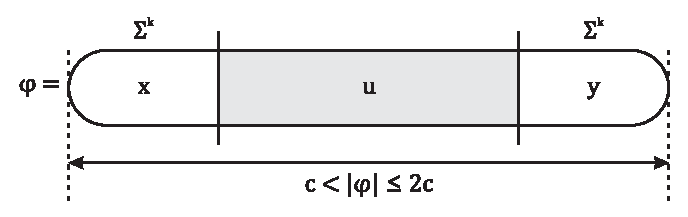
\includegraphics[scale=1.0]{img/instruction_phi.eps}
\caption[The illustration of the instruction $\phi$.]
%$\phi = (x, u \to \Delta^{m_0 + m_2 (i - 1) + j - 1}, y)$.]
{The illustration of the instruction $\phi = (x, u \to \Delta^{m_0 + m_2 (i - 1) + j - 1}, y)$.}
\label{figure:instruction_phi}
\end{figure}

We can easily generalize Lemma \ref{theorem:GsubseteqM} and Lemma \ref{theorem:MsubseteqG} to fit to our case and prove that $L_C(M) = L(G') \cup \{ \lambda \}$. We omit these obvious proofs and verify only that the resulting automaton $M$ has the desired properties. The properties \ref{request:m_0}, \ref{request:m_2} and \ref{request:k} can be easily verified. The only interesting property is the property \ref{request:m_1}. Consider any instruction $(x, u \to \Delta^{m_0 + m_2 (i - 1) + j - 1}, y) \in \Phi_2$, where $i \in \{1, 2, \ldots, m\}$ and $j \in \{1, 2, \ldots, m_2\}$. We know that $|x| = |y| = k$ and $|xuy| > c = U + m_1 - 1$. Therefore, $|u| \ge m_0 + m_1 + m_2 m - 1$. Since $m_0 + m_2 (i - 1) + j - 1 \le m_0 + m_2 m - 1$, we immediately get that $|u| - |\Delta^{m_0 + m_2 (i - 1) + j - 1}| \ge m_1$.

The following lemma will be important later:

\begin{lemma}\label{lemma:dxclra_t}
For each $t \ge 1$, we can set the parameters $m_1$ and $k$ in such a way, that for each instruction $(x, u \to \Delta^r, y) \in \Phi_2$, there exists a subword $v \in \Sigma^*$ (not containing $\Delta$) in the word $u$ with the length $|v| \ge t$. Moreover, $m_1, k = \Theta(t)$. The parameters $m_0$ and $m_2$ can be chosen arbitrarily.
\end{lemma}

\begin{proof}
Set $k := t$ and $m_1 := 2 t + m_2 m - 1$. Consider any instruction $(x, u \to \Delta^r, y) \in \Phi_2$. If $u \in \Sigma^*$ then $v := u$ and we obtain $|v| = |u| > m_1 > t$. Suppose that there are some letters $\Delta$ in $u$. If we can find two consecutive continuous sequences of letters $\Delta$ in $u$, then at least $k$ letters from $\Sigma$ separate these two sequences. We can set $v$ to be this separator. Suppose that there is only one continuous sequence of letters $\Delta$, i.\,e.\ $u = w_1 \Delta^s w_2$ for some $w_1, w_2 \in \Sigma^*$. We know that $|w_1| + s + |w_2| - r \ge m_1$. On the other hand, $|w_1| + s + |w_2| - r \le |w_1| + |w_2| + m_2 m - 1$, since $m_0 \le r, s \le m_0 + m_2 m - 1$. Accordingly, $|w_1| + |w_2| + m_2 m - 1 \ge m_1$. The longer of the words $w_1$, $w_2$ has the length at least $\frac{1}{2}(m_1 - m_2 m + 1) = t$.
\end{proof}

In the following, we outline the basic idea behind the transformation of a $\DXclRA$ $M$ obtained from the previous construction into an equivalent $\DclRA$ $N$. First suppose that we do this transformation in a trivial way, i.\,e.\ we transform each instruction $\phi = (x, u \to \Delta^r, y)$ of $M$, where $r > 1$ and $u = u_1 \ldots u_s$, into the following set of so-called \emph{partial instructions}:
$$
\begin{array}{ll}
\phi_1 & = (x, \underline{u_1} \to \Delta, u_2 u_3 \ldots u_s y),\\
\phi_2 & = (x \Delta, \underline{u_2} \to \Delta, u_3 u_4 \ldots u_s y),\\
\ldots\\
\phi_{r-1} & = (x \Delta^{r-2}, \underline{u_{r-1}} \to
\Delta, u_r u_{r+1} \ldots u_s y),\\
\phi_r & = (x \Delta^{r-1}, \underline{u_r u_{r+1} \ldots u_s} \to \Delta, y).
\end{array}
$$
Apparently, this technique gives us only the inclusion $L(M) \subseteq L(N)$. The other inclusion is not guaranteed. The problem is that we can find two different instructions $\phi$ and $\psi$ in $M$ such that they have different partial instructions $\phi_i$ and $\psi_j$ applicable in the same context. One possible way how to avoid such situations is to introduce some new special instructions, which will encode some extra information into $u$ by rewriting some letters with auxiliary $\Delta$-symbols. By using Lemma \ref{lemma:dxclra_t} we can guarantee a long enough subword $v \in \Sigma^*$ in $u$, which we can use to encode this information. In the rest of this section we describe how to accomplish this task by using one specific coding. Before we jump into the description of the coding, we introduce a useful algorithmic viewpoint, which resembles interactive protocols or even Arthur-Merlin games from the complexity theory. This viewpoint will later simplify many complex constructions used in this section.

\subsection{Algorithmic Viewpoint}\label{section:dxclra_viewpoint}

Let $\Sigma$ be an input alphabet not containing the sentinels $\cent$ and $\$$. Consider two nondeterministic machines: the \emph{querier} $Q$, the \emph{solver} $S$, and the \emph{protocol} \ref{algorithm:dxclra_protocol}.

\begin{algorithm}
\SetKwInOut{Input}{Input}\SetKwInOut{Output}{Output}
\caption{Protocol for the querier $Q$ and the solver $S$.}
\label{algorithm:dxclra_protocol}
\DontPrintSemicolon
\LinesNumbered
\Input{Word $u \in \Sigma^*$.}
\nonl Let $w \leftarrow \cent \cdot u \cdot \$$.\;
\nonl \While{\textbf{true}}{
Ask the querier $Q$ to choose a subword $x$ of $w$, i.\,e.\ $w = w_1 x w_2$.\;
If the solver $S$ accepts $x$ then \textbf{Accept} and \textbf{Halt}.\;
If the solver $S$ answers $y$ on the input $x$ then $w \leftarrow w_1 y w_2$.\;}
\end{algorithm}

The protocol $(Q, S)$ accepts a word $u$ if and only if there exists an accepting computation. Let $L(Q, S)$ denotes the language recognized by the protocol $(Q, S)$:
$$L(Q, S) = \{\ u\ \mid \text{ protocol } (Q, S) \text{ accepts } u\ \}.$$

Consider a class of queriers $\calQ$ and a class of solvers $\calS$. Then $\calL{\calQ, \calS}$ denotes the class of languages recognized by these queriers and solvers:
$$\calL{\calQ, \calS} = \{\ L(Q, S)\ \mid\  Q \in \calQ, S \in \calS\ \}.$$

In the following we will consider only the class of queriers $\calQ = \{Q_1, Q_2, \ldots\}$, such that each querier $Q_K \in \calQ$ for the given input word $w$ chooses nondeterministically an arbitrary subword $x$ of the word $w$ of the length $|x| \le K$.

The only constraint we put on the solver $S$ is that it should preserve the sentinels $\cent$ and $\$$. In other words, the solver can neither erase these sentinels, nor create new ones. We are not interested in the time or space complexity of the solver $S$.

On the other hand, depending on the additional constraints that we put on the solvers we can obtain different classes of solvers, and therefore also different classes of languages $\calL{\calQ, \calS}$. In the following we list several examples.

\begin{enumerate}
\item\label{solver:cl}
Consider the class of solvers $\calS_{cl}$, such that each solver $S \in \calS_{cl}$ works according to the following schema:
\begin{enumerate}
\item \label{solver:c1:a}
      if the input word $x = \cent \cdot \lambda \cdot \$$ then
      \textbf{Accept},
\item \label{solver:c1:b}
      otherwise, either \textbf{Reject}, or return $y$, which can be
      obtained from $x$ by deleting some subword of $x$ (and
      preserving the sentinels $\cent$ a $\$$).
\end{enumerate}
It is easy to see that $\calL{\calQ, \calS_{cl}} = \calL{\clRA}$.

The inclusion $\calL{\clRA} \subseteq \calL{\calQ, \calS_{cl}}$ is trivial. Suppose that $M = (\Sigma, \Phi)$ is a $\clRA$. Let $K = |M|$ be the maximal width of instructions of $M$. The solver $S$ will work according to the above schema in such a way that it will erase a substring from the given input word $x$ only if there exists an instruction of the automaton $M$ which allows such erasing. Apparently, $L(Q_K, S) = L(M)$. For the proof of the other inclusion $\calL{\calQ, \calS_{cl}} \subseteq \calL{\clRA}$ we use the fact the the querier only asks queries with the length bounded above by some constant $K$. Suppose that we have a protocol $(Q_K, S)$, where the solver $S$ works according to the above schema. There exist only finite many different queries the querier $Q_K$ may ask. For each such query $x$ we can describe the behavior of the solver $S$ on the input $x$ by using only the instruction of clearing restarting automata. If we unite all such instructions over all the queries the querier $Q_K$ may ask then we get the required $\clRA$ $M$, such that $L(M) = L(Q_K, S)$.

\item\label{solver:dcl}
The class $\calS_{\Delta cl}$ consists of such solvers $S$ that work according to the same schema as presented in \ref{solver:cl} with the only exception: in the case \ref{solver:c1:b}, the solver $S$ can leave a mark $\Delta \notin \Sigma$ at the place of deleting. Apparently, $\calL{\calQ, \calS_{\Delta cl}} = \calL{\DclRA}$.

\item\label{solver:dxcl}
By analogy, consider the class $\calS_{\Delta^* cl}$ which consists of solvers working according to the schema presented in \ref{solver:cl} with the only exception: in the case \ref{solver:c1:b} the solver $S$ can leave a continuous segment $\Delta^r$ at the place of deleting, where $\Delta \notin \Sigma$ and $r$ is bounded from above by the length of the deleted subword. Not surprisingly, $\calL{\calQ, \calS_{\Delta^* cl}} = \calL{\DXclRA}$.

\item\label{solver:cfl}
The class $\calS_{\textsf{CFL}}$ consists of such solvers $S$ that work according to the following schema:
\begin{enumerate}
\item \label{solver:cfl:a}
      if $x = \cent \cdot N_1 \cdot \$$ then \textbf{Accept},
\item \label{solver:cfl:b}
      if $x$ contains $\cent$ or $\$$ then \textbf{Reject},
\item \label{solver:cfl:c}
      if $x$ contains neither $\cent$, nor $\$$, then either
      \textbf{Reject}, or return a nonterminal.
\end{enumerate}
We prove that $\calL{\calQ, \calS_{\textsf{CFL}}} = \CFL$.

$\CFL \subseteq \calL{\calQ, \calS_{\textsf{CFL}}}$: Let $G = (V_N, V_T, N_1, P)$ be a context-free grammar with $V_N = \{N_1, \ldots, N_m\}$, and $\cent, \$ \notin V_N \cup V_T$. Let $K$ be the length of the longest right-hand side of productions from $P$. The corresponding solver $S$ will work according to the above schema in such a way, that in the case \ref{solver:cfl:c} $S$ returns the nonterminal $N_i$ only if $(N_i \to x) \in P$. Apparently, $L(Q_K, S) = L(G)$.

$\calL{\calQ, \calS_{\textsf{CFL}}} \subseteq \CFL$: There exist only finite many different queries the querier $Q_K$ may ask. For each such query $x$ we can describe the behavior of the solver $S$ on the input $x$ by using context-free productions of the form $(N_i \to x)$. If we unite all such productions over all the queries the querier $Q_K$ may ask then we get the required context-free grammar $G$, such that $L(G) = L(Q_K, S)$.

\item\label{solver:csl}
The class $\calS_{\textsf{CSL}}$ consists of such solvers $S$ that work according to the same schema as presented in \ref{solver:cfl} with the only exception: in the case \ref{solver:cfl:c}, the solver $S$ can rewrite any subword of the input word $x$ to a nonterminal $N_i$. Analogously, $\calL{\calQ, \calS_{\textsf{CSL}}} = \CSL$.
\end{enumerate}

In this way we can characterize also other language classes, such as pure languages \cite{maurer1980pure} etc. However, the most important contribution of these protocols is that we no longer perceive $\clRA$ ($\DclRA$, $\DXclRA$, respectively) as a mere set of instructions, but rather as a nondeterministic machine $S$ with an unbounded computational power working according to a particular schema. Instead of giving a list of instructions we rather describe the algorithm behind the corresponding solver. Now consider a $\DXclRA$ whose construction was based on a given context-free grammar $G$. Our goal is to construct a solver $S \in \calS_{\Delta cl}$, which will be able to imitate the work of the automaton $M$ by splitting every instruction of $M$ into several steps. In the first phase, the solver $S$ will encode (by using a special coding) some information into the tape specifying which instruction of $M$ it is going to execute. In the second phase, the solver $S$ will actually execute the chosen instruction (step by step). The coding will be designed in such a way that it will be possible to unambiguously interpret the content of the input tape at any given time.

\subsection{Coding}\label{section:dxclra_coding}

Consider a finite nonempty alphabet $\Sigma$ and $\Delta \notin \Sigma$. Our goal is to describe a mechanism which would enable us to encode any information to an arbitrary, sufficiently long word $w \in \Sigma^*$, only by replacing some letters of $w$ by symbols $\Delta$. Moreover, we require that it should be possible to recover the original word $w$ at any time.

\begin{theorem}[Coding 1]\label{theorem:dxclra_coding_1}
Let $\Sigma$ be a finite nonempty alphabet and $\Delta \notin \Sigma$. Then there exist a positive integer $B$ and a table $T$ of triples $(x, z, y)$, $xzy \in \Sigma^B$, $z \in \Sigma$, such that:
\begin{enumerate}
\item\label{theorem:dxclra_coding_1:a} $\{ xzy \mid (x, z, y) \in T \} = \Sigma^B$,
\item\label{theorem:dxclra_coding_1:b} For every $(x, y)$, $xy \in \Sigma^{B-1}$ there exists exactly one $z \in \Sigma: (x, z, y) \in T$.
\end{enumerate}
\end{theorem}

This theorem guarantees that if we take any word $w \in \Sigma^B$ then there exists a factorization $w = xzy$, such that $(x, z, y) \in T$. Now if we replace the letter $z$ by $\Delta$, we do not lose any information, since we are able to recover the letter $z$ from the context $(x, y)$ by using the table $T$.

\begin{proof}
Let us set $B = |\Sigma|$ and define a bipartite graph $G = (U \cup V, E)$ as follows:
\begin{enumerate}
\item $U = \Sigma^B$,
\item $V = (\Sigma \cup \{\Delta\})^B \cap (\Sigma^* \cdot \Delta \cdot \Sigma^*)$,
\item $E = \{ \{u, v\} \mid u \in U, v \in V, u = xzy, v = x \Delta y\}$.
\end{enumerate}
There is an edge $\{u, v\} \in E$ between $u \in U$ and $v \in V$ if and only if $v$ can be obtained from $u$ by replacing one of its letters by the symbol $\Delta$ (see Figure \ref{figure:graph}).
\begin{figure}[htp]
\centering
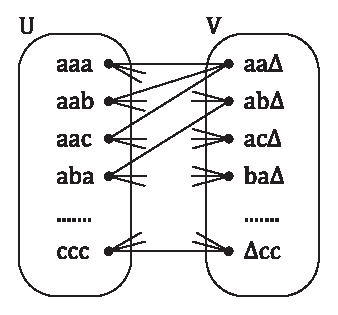
\includegraphics[scale=1.0]{img/graph.eps}
\caption[Bipartite graph $G = (U \cup V, E)$ for $\Sigma = \{a, b, c\}$.]
{Bipartite graph $G = (U \cup V, E)$ for $\Sigma = \{a, b, c\}$.}
\label{figure:graph}
\end{figure}
It is easy to see, that:
\begin{enumerate}
\item $|U| = |\Sigma^B| = B^B$,
\item $|V| = B |\Sigma|^{B-1} = B^B$.
\end{enumerate}
Moreover, the degree of each $u \in U$ in $G$ is $B = |\Sigma|$ and the degree of each $v \in V$ in $G$ is $|\Sigma|$. Therefore, $G$ is a $|\Sigma|$-regular bipartite graph. According to Hall's Theorem \cite{Hall1935} there exists a perfect matching in $G$, which gives us the required table $T$.
\end{proof}

\begin{example}\label{example:dxclra_ab}
Consider $\Sigma = \{a, b\}$. The adjacency matrix of the corresponding bipartite graph $G$ used in the proof of Coding 1 Theorem \ref{theorem:dxclra_coding_1} is shown in Table \ref{table:dxclra_example:dxclra_ab}.
\begin{table}[ht]
\centering
\begin{tabular}{| c || c | c | c | c |}
 \hline
     &  $a \Delta$  &   $b \Delta$&  $\Delta a$  &  $\Delta b$  \\
\hline\hline
$aa$ & $\mathbf{\underline{1}}$ &      $0$     &      $1$     &    $0$\\
\hline
$ab$ &      $1$     &      $0$     &      $0$     & $\mathbf{\underline{1}}$\\
\hline
$ba$ &      $0$     &      $1$     & $\mathbf{\underline{1}}$ &    $0$\\
\hline
$bb$ &      $0$     & $\mathbf{\underline{1}}$ &      $0$     &    $1$\\
\hline
\end{tabular}
\caption{Adjacency matrix for $\Sigma = \{a, b\}$.}
\label{table:dxclra_example:dxclra_ab}
\end{table}
The highlighted perfect matching gives us the following bijection:
$$aa \leftrightarrow a \Delta,
\ \ ab \leftrightarrow \Delta b,
\ \ ba \leftrightarrow \Delta a,
\ \ bb \leftrightarrow b \Delta,$$
and the corresponding table $T = \{
\ (a, a, \lambda),
\ (\lambda, a, b),
\ (\lambda, b, a),
\ (b, b, \lambda)\ \}$.
\end{example}
\begin{example}\label{example:dxclra_abc}
For $\Sigma = \{a, b, c\}$ we only give the resulting bijection:
\begin{center}
\begin{tabular}{lllll}
  $aaa \leftrightarrow \Delta a a$,\quad\quad
& $aab \leftrightarrow \Delta a b$,\quad\quad
& $aac \leftrightarrow a a \Delta$,\quad\quad
& $aba \leftrightarrow \Delta b a$,\quad\quad
& $abb \leftrightarrow a \Delta b$,\\
  $abc \leftrightarrow a b \Delta$,
& $aca \leftrightarrow a \Delta a$,
& $acb \leftrightarrow a c \Delta$,
& $acc \leftrightarrow a \Delta c$,
& $baa \leftrightarrow b \Delta a$,\\
  $bab \leftrightarrow b \Delta b$,
& $bac \leftrightarrow b a \Delta$,
& $bba \leftrightarrow b b \Delta$,
& $bbb \leftrightarrow \Delta b b$,
& $bbc \leftrightarrow \Delta b c$,\\
  $bca \leftrightarrow \Delta c a$,
& $bcb \leftrightarrow b c \Delta$,
& $bcc \leftrightarrow b \Delta c$,
& $caa \leftrightarrow c \Delta a$,
& $cab \leftrightarrow c a \Delta$,\\
  $cac \leftrightarrow \Delta a c$,
& $cba \leftrightarrow c b \Delta$,
& $cbb \leftrightarrow c \Delta b$,
& $cbc \leftrightarrow c \Delta c$,
& $cca \leftrightarrow c c \Delta$,\\
  $ccb \leftrightarrow \Delta c b$,
& $ccc \leftrightarrow \Delta c c$.
\end{tabular}
\end{center}

Next consider the following sample word:
$$w = acc bab cca caa bbc abc bca caa.$$
Let us factorize this word $w$ into the groups consisting of $B = 3$ letters:
$$w\ =\ acc\ \mid\ bab\ \mid\ cca\ \mid\ caa\ \mid\ bbc\ \mid\ abc\ \mid\ bca\ \mid\ caa.$$
Suppose that we want to encode the information $i = 11001010$ into the word $w$ without losing any information. We can achieve this by \emph{marking} the groups of $w$ by $\Delta$ that correspond to $1$s in the information $i$. If we use the above bijection we will be able to recover the original word $w$. After encoding the information $i$ we get the following word:
$$w'\ =\ a \Delta c\ \mid\ b \Delta b\ \mid\ c c a\ \mid\ c a a\ \mid
       \ \Delta b c\ \mid\ a b c\ \mid\ \Delta c a\ \mid\ c a a.$$
\end{example}

By applying the encoding from Example \ref{example:dxclra_abc} we can store an $n$-bit information in any word $w$ of length at least $n B$. However, we need to ``see'' the whole word $w$ in order to correctly define the groups of $B$ letters.

The perfect matching of a regular bipartite graph $G$ can be found effectively with respect to the size of the graph $G$. However, the table defining the bijection contains $|\Sigma|^{|\Sigma|}$ entries.  The question is, whether we can compute the bijection in polynomial time w.r.t. $|\Sigma|$ without precomputing the whole table $T$? The answer is yes. Let us assign to every $a \in \Sigma$ some value $\nu(a) \in \{1, \ldots, |\Sigma|\}$ bijectively, and define $\nu^*(w_1 \ldots w_n) = \sum_{i = 1}^{n} \nu(w_i) \mod |\Sigma|$, for all $w_1 \ldots w_n \in \Sigma^*$. The table $T$ consists of all triples of the form $(x, z, y)$, where $x, y \in \Sigma^*$, $z \in \Sigma$, $|xzy| = |\Sigma|$, and $\nu^*(xzy) = |x|$. Given any $w \in \Sigma^{|\Sigma|}$ we can effectively factorize $w$ to $xzy$, such that $(x, z, y) \in T$, by defining $|x| = \nu^*(w)$. This proves that $\{ xzy \mid (x, z, y) \in T \} = \Sigma^{|\Sigma|}$. Since $z$ is uniquely determined by the contexts $(x, y)$, $T$ satisfies both conditions \ref{theorem:dxclra_coding_1:a}, \ref{theorem:dxclra_coding_1:b} of Theorem \ref{theorem:dxclra_coding_1}, and we do not need to store it explicitly.

As we can see, the coding introduced in Coding 1 Theorem \ref{theorem:dxclra_coding_1} is \emph{length-preserving}. It means, that if we encode an information into a word $w$, the length of the word remains preserved. The question is, whether we can find a \emph{length-reducing} coding. The answer is: yes, trivially. Consider the following word:
$$w = ababaababbbaabaa.$$
First, we group together consecutive letters of $w$:
$$w = \underline{ab}\ \underline{ab}\ \underline{aa}
\ \underline{ba}\ \underline{bb}\ \underline{ba}
\ \underline{ab}\ \underline{aa}.$$
Now consider the word $w$ as a word over the \emph{pair} alphabet:
$$\underline{\Sigma} = \{\underline{aa}, \underline{ab},
\underline{ba}, \underline{bb}\}.$$
If we apply the length-preserving coding of Coding 1 Theorem \ref{theorem:dxclra_coding_1} on the pair alphabet $\underline{\Sigma}$, we automatically get a length-reducing coding over the original alphabet $\Sigma$. This is because the rewriting of one letter from the pair alphabet $\underline{\Sigma}$ by $\Delta$ is equivalent to the rewriting of two letters from the original alphabet $\Sigma$ by $\Delta$. However, in this case $B = 2|\underline{\Sigma}| = 2|\Sigma|^2$. For example, for $\Sigma = \{a, b\}$ we need groups of $B = 2|\Sigma|^2 = 8$ letters. Can we do better? The answer is: yes, but not too much.

\begin{theorem}[$\kappa$-Reducing Coding 1]
\label{theorem:dxclra_k_reducing_coding_1}
Let $\kappa$ be a nonnegative integer, $\Sigma$ a finite nonempty alphabet and $\Delta \notin \Sigma$. Then there exist a positive integer $B$ and a table $T$ of triples $(x, z, y)$, $xzy \in \Sigma^B$, $z \in \Sigma^{\kappa+1}$, such that:
\begin{enumerate}
\item\label{theorem:dxclra_k_reducing_coding_1:a} $\{ xzy \mid (x, z, y) \in T \} = \Sigma^B$,
\item\label{theorem:dxclra_k_reducing_coding_1:b} For every $(x, y)$, $xy \in \Sigma^{B-\kappa-1}$ there exists exactly one $z \in \Sigma^{\kappa+1}$ such that $(x, z, y) \in T$.
\end{enumerate}
\end{theorem}

\begin{proof}
Again, consider a bipartite graph $G = (U \cup V, E)$, where:
\begin{enumerate}
\item $U = \Sigma^B$,
\item $V = (\Sigma \cup \{\Delta\})^{B-\kappa} \cap (\Sigma^* \cdot \Delta \cdot \Sigma^*)$,
\item $E = \{ \{u, v\} \mid u \in U, v \in V, u = xzy, v = x \Delta y\}$.
\end{enumerate}
There is an edge $\{u, v\} \in E$ between $u \in U$ and $v \in V$ if and only if $v$ can be obtained from $u$ by replacing one of its subwords $z \in \Sigma^{\kappa+1}$ by $\Delta$. If we define $B = |\Sigma|^{\kappa+1} + \kappa$ then we get the equality $|U| = |V|$, because:
\begin{enumerate}
\item $|U| = |\Sigma^B| = |\Sigma|^B$,
\item $|V| = (B - \kappa) |\Sigma|^{B - \kappa - 1} = |\Sigma|^{\kappa+1} |\Sigma|^{B - \kappa - 1} = |\Sigma|^B$.
\end{enumerate}
Moreover, the degree of each $u \in U$ in $G$ is $B - \kappa = |\Sigma|^{\kappa+1}$ and the degree of each $v \in V$ in $G$ is $|\Sigma|^{\kappa+1}$. Therefore, $G$ is a $|\Sigma|^{\kappa+1}$-regular bipartite graph. According to Hall's Theorem \cite{Hall1935} there exists a perfect matching in $G$, which gives us the required table $T$.
\end{proof}

For example, for $\Sigma = \{a, b\}$ the $1$-Reducing Coding 1 gives us $B = |\Sigma|^{\kappa+1} + \kappa = 5$, which is an improvement to $B = 8$.

The obvious problem with Coding 1 is that we need to ``see'' the whole word $w$ in order to correctly define the groups of $B$ letters. One possible way how to avoid this problem is to find a coding that is not dependent on any specific factorization of the word to the groups of letters. Our goal is to recover the original letters hidden by the symbols $\Delta$ only with the knowledge of local contexts of these symbols $\Delta$.

\begin{theorem}[Coding 2]\label{theorem:dxclra_coding_2}
Let $\Sigma$ be a finite nonempty alphabet and $\Delta \notin \Sigma$. Then there exist positive integers $B$, $K$, and a table $T$ of triples $(x, z, y)$, $x, y \in \Sigma^K$, $z \in \Sigma$, such that:
\begin{enumerate}
\item\label{theorem:dxclra_coding_2:a}
For every context $(x, y) \in \Sigma^K \times \Sigma^K$ there exists at most one $(x, z, y) \in T$.
\item\label{theorem:dxclra_coding_2:b} For every word $w \in \Sigma^B$ there exists at least one $(x, z, y) \in T$ such that $xzy$ is a subword of $w$.
\end{enumerate}
\end{theorem}

Apparently, we can replace the letter $z$ by $\Delta$ in the subword $xzy$ of $w$ without losing any information, because we can recover $z$ from the context $(x, y)$.

\begin{proof}
(Induction by $|\Sigma|$). For $\Sigma = \{a, b\}$ let us set $B = 8$, $K = 2$, and
\begin{center}
\begin{tabular}{c c c c c c}
$T = \{$ &
   $(aa, a, aa)$,& $(ab, a, aa)$,& $(ba, b, aa)$,& $(bb, a, aa)$,& \\
 & $(aa, a, ab)$,& $(ab, a, ab)$,& $(ba, b, ab)$,& $(bb, a, ab)$,& \\
 & $(aa, b, ba)$,& $(ab, a, ba)$,& $(ba, b, ba)$,& $(bb, b, ba)$,& \\
 & $(aa, b, bb)$,& $(ab, a, bb)$,& $(ba, b, bb)$,& $(bb, b, bb)$ & $\}\;.$\\
\end{tabular}
\end{center}
The condition \ref{theorem:dxclra_coding_2:a} obviously holds. The condition
\ref{theorem:dxclra_coding_2:b} is verified in Table \ref{table:dxclra_verify2}.

\begin{table}[ht]
\centering
\begin{tabular}{c c c c}
\hline \hline
\underline{aaaaa}??? & \underline{aaaab}??? &
aa\underline{abaaa}? & aa\underline{abaab}?\\
aa\underline{ababa}? & aa\underline{ababb}? &
a\underline{aabba}?? & a\underline{aabbb}??\\
a\underline{abaaa}?? & a\underline{abaab}?? &
a\underline{ababa}?? & a\underline{ababb}??\\
\underline{aabba}??? & \underline{aabbb}??? &
\underline{abaaa}??? & \underline{abaab}???\\
\underline{ababa}??? & \underline{ababb}??? &
a\underline{bbaaa}?? & a\underline{bbaab}??\\
ab\underline{babaa}? & ab\underline{babab}? &
ab\underline{babba}? & ab\underline{babbb}?\\
ab\underline{bbaaa}? & ab\underline{bbaab}? &
abb\underline{babaa} & abb\underline{babab}\\
abb\underline{babba} & abb\underline{babbb} &
a\underline{bbbba}?? & a\underline{bbbbb}??\\
b\underline{aaaaa}?? & b\underline{aaaab}?? &
baa\underline{abaaa} & baa\underline{abaab}\\
baa\underline{ababa} & baa\underline{ababb} &
ba\underline{aabba}? & ba\underline{aabbb}?\\
ba\underline{abaaa}? & ba\underline{abaab}? &
ba\underline{ababa}? & ba\underline{ababb}?\\
b\underline{aabba}?? & b\underline{aabbb}?? &
\underline{babaa}??? & \underline{babab}???\\
\underline{babba}??? & \underline{babbb}??? &
\underline{bbaaa}??? & \underline{bbaab}???\\
b\underline{babaa}?? & b\underline{babab}?? &
b\underline{babba}?? & b\underline{babbb}??\\
b\underline{bbaaa}?? & b\underline{bbaab}?? &
bb\underline{babaa}? & bb\underline{babab}?\\
bb\underline{babba}? & bb\underline{babbb}? &
\underline{bbbba}??? & \underline{bbbbb}???\\
\hline
\end{tabular}
\caption{All possibilities for $w \in \Sigma^K$.}
\label{table:dxclra_verify2}
\end{table}

Note that $T$ can be shortly described as $T = \{ (xx, y, y?) \mid x, y \in \Sigma \} \cup \{ (xy, x, ??) \mid x \neq y; x, y \in \Sigma \}$,  where the symbol $?$ is a placeholder for an arbitrary letter from $\Sigma$. We can avoid using the symbol $?$ completely by writing $T = \{ (xx, y, y) \mid x, y \in \Sigma \} \cup \{ (xy, x, \lambda) \mid x \neq y; x, y \in \Sigma \}$. In other words, we allow using triples $(l, z, r)$, where $|l| < K$ or $|r| < K$ (or both). This is not a problem since we can easily extend the left context (right context, respectively) to be from $\Sigma^K$ by adding (all possible combinations of) ``dummy'' letters from $\Sigma$ to the left of the left context $l$ (to the right of the right context $r$, respectively). The reason why $T$ satisfies the condition \ref{theorem:dxclra_coding_2:b} is as follows. Consider a sufficiently long word $w \in \Sigma^*$. There are only two cases: either each (internal) letter in $w$ is doubled, i.\,e.\ each (internal) letter $x$ in $w$ has a neighbor $x$, or there exists an (internal) letter $x$ in $w$ which does not have a neighbor $x$. In the first case the pattern $xxyy$ will occur, and in the second case the pattern $xyx$, where $x \neq y$, will occur.

The proof of the induction step was provided by a Russian mathematician Ilya Bogdanov on the following website: \url{http://mathoverflow.net/questions/76326/can-you-hide-a-letter-without-losing-information}. Let us assume that we know the positive integers $B'$, $K'$, and the table $T'$ of triples for some alphabet $\Sigma'$. Our goal is to find the positive integers $B$, $K$, and the table $T$ of triples (satisfying both conditions  \ref{theorem:dxclra_coding_2:a}, \ref{theorem:dxclra_coding_2:b}) for the extended alphabet $\Sigma = \Sigma' \cup \{x\}$, where $x \notin \Sigma'$. Let us assume that $K' \ge 2|\Sigma'|$. We claim that we can set $K = B'$. For convenience, we say that we \emph{catch} the word $w \in \Sigma^*$ if there exists at least one $(x, z, y) \in T$ such that $xzy$ is a subword of $w$ (i.\,e.\ the condition \ref{theorem:dxclra_coding_2:b} holds for the word $w$). Our goal is to catch all long enough words (i.\,e.\ all words from $\Sigma^B$ for some positive integer $B$). First, let us reuse all triples from $T'$, except that we need to prolong their contexts to the length $K$. By using the triples from $T'$ we can catch every word $w \in \Sigma^*$ that contains a subword $w'$ over $\Sigma'$ of  length at least $B'$ (where this subword stands at least $K$ letters from the beginning of the word $w$ to leave enough room for the prolonged contexts). Second, we need to catch also all other words. These words contain subwords of the form $xw'x$, where $0 \le |w'| < B'$ and $w'$ does not contain $x$ (again we consider only subwords $xw'x$ standing at least $K$ letters from the beginning). Let $xw'x$ be any such subword with the maximal possible length. We distinguish three cases: (1) $|w'|$ is at least $2 |\Sigma'|$, (2) $|w'|$ is at least $|\Sigma'|$, but less than  $2 |\Sigma'|$, and (3) $|w'|$ is less then $|\Sigma'|$.
\begin{enumerate}
\item[(1)] In case $|w'| \ge 2 |\Sigma'|$ we can reuse the idea of Coding 1 (see Theorem \ref{theorem:dxclra_coding_1}). Let us assign to every $a \in \Sigma'$ some value $\nu(a) \in \{1, \ldots, |\Sigma'|\}$ bijectively, and define $\nu^*(w_1 \ldots w_n) = \sum_{i = 1}^{n} \nu(w_i) \mod |\Sigma'|$. Let us add to $T$ all triples of the form $(xu, a, vx)$, where $u, v$ are words over $\Sigma'$, $a \in \Sigma'$, $0 \le |u| < |\Sigma'|$, $|\Sigma'| \le |v| < B'$, $2|\Sigma'| \le |uav| < B'$, and $\nu^*(uav) = |u|$. Now if we have any subword $xw'x$ with $|w'| \ge 2 |\Sigma'|$, then we set $u$ to be the prefix of $w'$ of length $\nu^*(w')$, $a$ to be the next letter of $w'$, and $v$ to be the remaining suffix of $w'$. It is easy to see that $\nu^*(uav) = \nu^*(w') = |u|$, i.\,e.\ our word $w$ is caught by a triple $(xu, a, vx) \in T$. Since $a$ is determined uniquely by $u$ and $v$, these triples satisfy the condition \ref{theorem:dxclra_coding_2:a}.
\item[(2)] In case $|\Sigma'| \le |w'| < 2 |\Sigma'|$ we use the triples of the form $(xu, x, \lambda)$, where $u$ is over $\Sigma'$ and $|\Sigma'| \le |u| < 2 |\Sigma'|$. Note that these triples do not interfere with the triples from (1), because here $|\Sigma'| \le |u|$.
\item[(3)] Finally, if $|w'| < |\Sigma'|$ we use the triples of the form $(xu, x, vx)$, where $u, v$ are words over $\Sigma'$, and $0 \le |u|, |v| < |\Sigma'|$. These triples do not interfere with the triples from (1), because here we have $|v| < |\Sigma'|$. They do not interfere with the triples from (2), because here we have $|u| < |\Sigma'|$.
\end{enumerate}
To formally prove the condition \ref{theorem:dxclra_coding_2:a}, let $(l, r) \in \Sigma^K \times \Sigma^K$. If $\Suff_{2|\Sigma'|}(l)$ does not contain $x$, then only a triple from $T'$ can match the context $(l, r)$. This is because all triples from $T'$ have contexts of length $K' \ge 2|\Sigma'|$, and all other triples from $T$ contain $x$ in $\Suff_{2|\Sigma'|}(l)$. In (1) $\Suff_{|\Sigma'|}(l)$ contains $x$, while $\Pref_{|\Sigma'|}(r)$ does not. In (2) $\Suff_{2|\Sigma'|}(l)$ contains $x$, while $\Suff_{|\Sigma'|}(l)$ does not. Finally, in (3) both $\Suff_{|\Sigma'|}(l)$ and $\Pref_{|\Sigma'|}(r)$ contain $x$. It is easy to see that the condition \ref{theorem:dxclra_coding_2:b} is satisfied for long enough words. Let $B = 3B'$ and $w \in \Sigma^B$. If $w$ contains a subword $w'$ over $\Sigma'$ of length at least $B'$ standing at least $K = B'$ letters from the beginning, then it is caught by $T'$. Otherwise, it contains at least two consecutive subwords of the form $xw'x$ standing at least $K$ letters from the beginning, in which case one of the cases (1), (2), (3) applies.
\end{proof}

We will not use Coding 2 in our proof, because Coding 1 is more compact and much simpler. However, as we have already mentioned before, the problem with Coding 1 is that the solver $S \in \calS_{\Delta cl}$ may not be able to decode $\Delta$ symbols in the input word $w$, since $w$ can often be only a small part of the original input tape. If the word $w$ does not start with the left sentinel $\cent$ then we are not able to correctly factorize $w$ into the groups of $B$ letters, and thus we are not able to interpret $\Delta$ symbols occurring in the word $w$.

Fortunately, there exists a simple trick how to avoid this problem. In order to correctly factorize the input word $w$ into groups of $B$ letters we only need some kind of ``fixed point'', which exactly defines the starting position of the first group of the correct factorization. The left sentinel $\cent$ is one example of such fixed point. Thus in the first phase we distribute such fixed points throughout the whole input tape starting at the left sentinel $\cent$. The distances between two consecutive fixed points will be approximately constant. We illustrate this idea on the following simplified example. Suppose that we have the following word:
$$w = abacc \Delta bac bba cac bcb aac bcb acb aca bab$$
The symbol $\Delta$ in $w$ represents our fixed point and defines the following factorization:
$$w = abacc \mathbf{\Delta}\ \mid\ bac\ \mid\ bba\ \mid\ cac\ \mid\ bcb
\ \mid\ aac\ \mid\ bcb\ \mid\ acb\ \mid\ aca\ \mid\ bab$$
We place the next fixed point into the $9$th group to the right from the highlighted fixed point $\mathbf{\Delta}$ (by using the bijection from Example \ref{example:dxclra_abc}):
$$w' = abacc \Delta\ \mid\ bac\ \mid\ bba\ \mid\ cac\ \mid\ bcb\ \mid\ aac\ \mid\ bcb\ \mid\ acb\ \mid\ aca\ \mid\ b \Delta b$$
As you can see, the number of letters between two consecutive fixed points is either  $3 \times 8$, or $3 \times 8 + 1$, or $3 \times 8 + 2$. We place another fixed point whenever the input word $w$ is of the form $w \in \cent \cdot \Sigma^{\ge 3 \times 9}$ or $w \in \Sigma^* \cdot \Delta \cdot \Sigma^{\ge 3 \times 9}$.

\subsection{Idea of the Algorithm}\label{section:dxclra_algorithm}

In this section we describe the algorithm behind the solver $S \in \calS_{\Delta cl}$, which imitates the work of the $\DXclRA$ $M$ constructed according to a given context-free grammar in Chomsky normal form. The automaton $M$ works in a bottom-up fashion. If the automaton recognizes that some subword $w$ of the input tape can be derived from a nonterminal $N_i$, then it can replace the inner part of this subword $w$ by the code $\Delta^r$, where $r = m_0 + m_2 (i - 1) + j - 1$ for some $j \in \{1, 2, \ldots, m_2\}$, leaving the first $k$ letters and the last $k$ letters of $w$ as separators. The segment $\Delta^r$ together with its separators represents a code for the nonterminal $N_i$. These separators have a nice and useful property: if one changes some letters in these separators, the acceptance of the whole word on the input tape remains
unchanged.

Our solver $S$ is not obliged to preserve the representation used by the automaton $M$. Moreover, because of some technical reasons, we will not represent the nonterminal $N_i$ by using a continuous segment $\Delta^r$. Instead, we will use the segment $\Delta x \Delta^{r-4} y \Delta$, where $x, y \in \Sigma$ are the so-called ``holes''. These holes are useful in the sense that they can unambiguously identify the start and the end of the segment $\Delta x \Delta^{r-4} y \Delta$ inside any word marked by other symbols $\Delta$. For example, in the following word:
$$a \Delta c ca\Delta \underline{\Delta b \Delta^{r-4} a \Delta} aab$$
we have underlined such segment with holes. It will be clear later why we need this representation. For convenience, we will often use the following convention: whenever we talk about a \emph{continuous segment $\Delta^r$ with holes}, we will always mean the segment $\Delta x \Delta^{r-4} y \Delta$, where $x, y \in \Sigma$ represent the holes.

In the following we introduce another conventions which will be used later in the description of the resulting algorithm. As we have already explained, if we want to encode the information into some word $w \in \Sigma^*$, we need to know the factorization of this word $w$ into groups of $B$ letters (see Section \ref{section:dxclra_coding}). This factorization (once defined) cannot be changed during the course of the algorithm. Otherwise, we could misinterpret the symbols $\Delta$ occurring in the word $w$. In order to correctly factorize the input word we need to find the so-called \emph{fixed point}. We recognize three types of fixed points:

\begin{enumerate}
\item \emph{Fixed point $\cent$}: In the word $\cent \cdot w$, where $w \in \Gamma^*$, the fixed point $\cent$ defines the following groups:
$$\cent \mid w_1 \mid w_2 \mid w_3 \mid \ldots,$$
where $w = w_1 w_2 w_3 \ldots$, and $|w_1| = |w_2| = |w_3| = \ldots = B$. In other words, the start of the input tape is a fixed point.

\item \emph{Fixed point $\Delta^r$ with holes}: In the word $u w$, where $u$ is the segment $\Delta^r$ with holes, $r = m_0 + m_2 (i - 1) + j - 1$ for some $j \in \{1, 2, \ldots, m_2\}$, the fixed point $u$ defines the following groups:
$$w_0 \mid w_1 \mid w_2 \mid w_3 \mid \ldots,$$
where $u w = w_0 w_1 w_2 \ldots$, $|w_0| = m_0 + m_2 (i - 1)$, and $|w_1| = |w_2| = |w_3| = \ldots = B$. In other words, the segment $\Delta^r$ with holes is a fixed point. Note that $|w_0| \le r$. The reason why we factorize the word $u w$ in this way will be explained later.

\item \emph{Fixed point $\mathbf{u} \Delta \mathbf{v} \Delta$}: In the word $u \Delta v \Delta w$, where $u \in \Sigma^{2B}$, $v \in \Sigma^{\le 2B - 2}$, $w \in \Sigma \cdot \Gamma^*$, the fixed point $\mathbf{u} \Delta \mathbf{v} \Delta$ defines the following groups:
$$u \Delta v \Delta \mid w_1 \mid w_2 \mid w_3 \mid \ldots,$$
where $w = w_1 w_2 w_3 \ldots$, and $|w_1| = |w_2| = |w_3| = \ldots = B$. In other words, two symbols $\Delta$, which are close to each other, represent a fixed point.
\end{enumerate}

To prevent the accidental creation of fixed points of the type $\mathbf{u} \Delta \mathbf{v} \Delta$ we introduce the following convention. We do not encode the information straight into the groups of length $B$, but rather to the so-called \emph{units}. A unit is defined as three consecutive groups of length $B$. If we want to mark a unit in order to encode one bit of information we always mark the middle group of the unit. The first and the third group of the unit serves as separators. Thanks to these separators any two consecutive symbols $\Delta$ in any two neighboring units are separated by at least $2B$ letters from $\Sigma$. We illustrate this idea on the following example. Consider $\Sigma = \{a, b, c\}$ and the following word:
$$abc \Delta^r acc bab cca caa bbc abc bcc caa,$$
where $r = m_0 + m_2 (i - 1)$. The fixed point $\Delta^r$ (with holes) defines the following groups:
$$abc \Delta^r \mid \mid acc \mid \mathbf{bab} \mid cca \mid \mid caa \mid \mathbf{bbc} \mid abc \mid \mid bcc \mid caa,$$
where the units are separated by two lines ($\mid \mid$). The middle groups of the units are in bold.

Note that if we mark two consecutive units, we never get the fixed point of the type $\mathbf{u} \Delta \mathbf{v} \Delta$. However, we can always obtain such a fixed point by marking two consecutive groups, provided that there are at least two unmarked groups preceding the first marked group. We use this observation in the first phase of the algorithm, in which we distribute the fixed points of this type throughout the whole input tape.

In the following we introduce the term \emph{working area}. Consider an input tape with all its fixed points. If we erase these fixed points, the input tape will break into the segments, which we refer to as the working areas (see Figure \ref{figure:tape}).

\begin{figure}[htp]
\centering
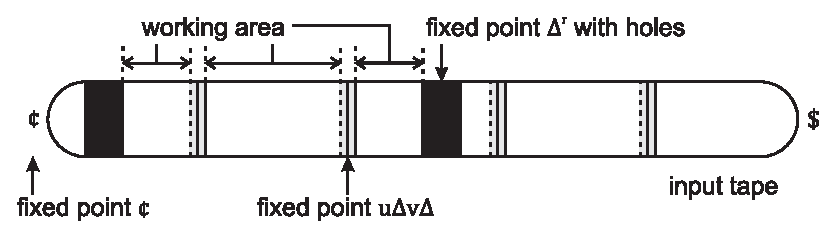
\includegraphics[scale=1.0]{img/tape.eps}
\caption[The segmentation of the input tape into the working areas.]
{The segmentation of the input tape into the working areas.}
\label{figure:tape}
\end{figure}

Fixed points exactly define the factorization into the groups of length $B$ and thus they also define the corresponding units inside these working areas. The term \emph{working space} refers to the longest possible subword of the working area containing only the whole units that can be used to encode some information (see Figure \ref{figure:working_space}).

\begin{figure}[htp]
\centering
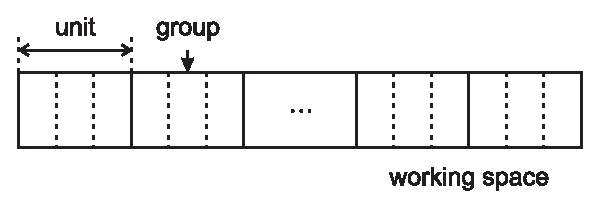
\includegraphics[scale=1.0]{img/working_space.eps}
\caption[Working space divided into the units.]
{Working space divided into the units.}
\label{figure:working_space}
\end{figure}

Since we encode the information only into the middle groups of the units, no fixed points can be created in this way. However, there is one special exception. During the computation the algorithm gets into a state in which it starts to create a new continuous segment $\Delta^r$ (with holes) somewhere inside the working space. This segment will (after completing) represent a code for a nonterminal. By definition, the completed segment $\Delta^r$ (with holes) represents also a new fixed point. This could be a problem, since the process of the execution of the instruction of the automaton $M$ is not yet completed at this stage. In order to finish this process we must also clear the remaining letters on both sides of the newly created segment $\Delta^r$ (with holes). The problem is, that a new fixed point could break the correctness of the previously defined factorization into the groups of length $B$. Therefore, in the following we introduce some new terms that will enable us to solve this problem.

The working area is called \emph{empty} if it does not contain a subword $u \Delta v$, where $u, v \in \Sigma^{4L}$. Otherwise we call the working area \emph{reserved}. Next, we will distinguish between \emph{valid} and \emph{invalid} fixed points. The fixed points of the types $\cent$ and $\mathbf{u} \Delta \mathbf{v} \Delta$ are always valid. The fixed point of the type $\Delta^r$ (with holes) is valid only if there exists at least one empty working area adjacent to this fixed point. Otherwise, the fixed point $\Delta^r$ (with holes) is invalid. Thus, if we want to make the fixed point $\Delta^r$ (with holes) invalid, we only need to place this fixed point between two marked units.

Now we are ready to give the details of the algorithm imitating the work of the $\DXclRA$ $M$ (see Algorithm \ref{algorithm:dxclra_solver}).

\begin{algorithm}
\SetKwInOut{Input}{Input}\SetKwInOut{Output}{Output}
\caption{Algorithm behind the solver $S \in \calS_{\Delta cl}$ imitating the work of the $\DXclRA$ $M = (\Sigma, \Phi)$.}
\label{algorithm:dxclra_solver}
\DontPrintSemicolon
\LinesNumbered
\Input{Word $w \in \{\lambda, \cent\} \cdot \Gamma^* \cdot \{\lambda, \$\}$.}
Find all fixed points inside $w$. Determine which of them are valid.\label{algorithm:dxclra_solver:step_1}\;
Let $w = z_0 o_0 z_1 o_1 \ldots z_d o_d$, where:\label{algorithm:dxclra_solver:step_2}\;
\nonl (a) $z_0$ is a fixed point (it may not be possible to decide if
it is valid),\;
\nonl (b) $z_1, \ldots, z_d$ are the (decidable) valid fixed points of $w$,\;
\nonl (c) $o_0, \ldots, o_d$ are the corresponding working areas in $w$.\;
\nonl The working area $o_d$ may contain the right sentinel $\$$.\\
\nonl If it is not possible to factorize $w$ in this way, especially if $w$ does not start with the fixed point, then $\textbf{Reject}$.\;
Identify the groups of length $B$ and the corresponding units in the working areas $o_1, \ldots, o_d$. If $z_0$ is a valid fixed point then take also the working area $o_0$ into consideration.\label{algorithm:dxclra_solver:step_3}\;
If the working area $o_d \in \Sigma^{\ge \textsf{const}} \cdot \{\lambda, \$\}$ (where $\textsf{const}$ will be specified later), then add another fixed point of the type $\mathbf{u} \Delta \mathbf{v} \Delta$ into this working area and $\textbf{Halt}$.\label{algorithm:dxclra_solver:step_4}\;
Recover all symbols $\Delta$ in the word $w$ that can be recovered. We use the notation $\bar{u}$ for the recovered word $u$.\label{algorithm:dxclra_solver:step_5}\;
If $\bar{w} = \cent \cdot \bar{u} \cdot \$$ and $(\cent, \bar{u} \to \lambda, \$) \in \Phi$, then $\textbf{Accept}$.\label{algorithm:dxclra_solver:step_6}\;
Otherwise, let $\phi = (x, u \to \Delta^r, y)$ be the instruction of $M$, which can be applied in the subword $z_{\alpha} o_{\alpha} \ldots z_{\beta} o_{\beta}$, where both $z_{\alpha}$ and $z_{\beta}$ are valid fixed points. More precisely, either there exists a reserved working area $o_{\gamma}$ ($\alpha \le \gamma \le \beta$), in which it is exactly encoded, which instruction $\phi$ is being executed in this area, or there is no such working area and $xuy$ is a subword of the word $\bar{z}_{\alpha} \bar{o}_{\alpha} \ldots \bar{z}_{\beta} \bar{o}_{\beta}$ (Even if there was a reserved working area $o_{\gamma}$, then the encoding process in this area might not be finished, which would automatically imply that all its $\Delta$ symbols can be recovered). In the case that all the working areas $o_{\alpha}, \ldots, o_{\beta}$ are empty, we only need to choose one of them. We know that in the word $u$ there exists a sufficiently long subword $v \in \Sigma^*$ in which we can encode the information. Suppose that $v$ covers the working area $o_{\gamma}$, where $\alpha \le \gamma \le \beta$. Then we choose $o_{\gamma}$ if both of the following two conditions hold:\\
\nonl (a) Either $\gamma = \alpha = 0$ and $z_0 = \cent$, or $\gamma > \alpha \ge 0$,\\
\nonl (b) Either $\gamma = \beta = d$ and $o_d$ ends with sentinel $\$$, or $\gamma < \beta \le d$.\\
\nonl If there is no such instruction then $\textbf{Reject}$.\label{algorithm:dxclra_solver:step_7}\;
Execute one step of the execution of the instruction $\phi$ and $\textbf{Halt}$.\label{algorithm:dxclra_solver:step_8}\;
\end{algorithm}

Step \ref{algorithm:dxclra_solver:step_1} is clear. Fixed points are exactly defined nonoverlapping segments (we suppose that $m_0 \ge 8$). If we delete these segments the input word $w$ will break into the areas. These areas enable us to determine which fixed points are valid and which are not. The only exception is the first fixed point $z_0$. If $z_0$ is of the type $\Delta^r$ (with holes) then we may not be able to decide if $z_0$ is a valid fixed point, since we do not see to the left of $z_0$. We always suppose that the input word $w$ starts with a fixed point (otherwise, we reject). Valid fixed points exactly define both the factorization $w = z_0 o_0 z_1 o_1 \ldots z_d o_d$ in Step \ref{algorithm:dxclra_solver:step_2}, and the groups of length $B$ and the corresponding units in Step \ref{algorithm:dxclra_solver:step_3}. Thanks to these factorizations we are able to recover the symbols $\Delta$ occurring in the word $w$. If $u$ is a subword of $w$ then we denote by $\bar{u}$ the word $u$ with all possible symbols $\Delta$ occurring in $u$ recovered. We may not be able to recover all the symbols $\Delta$ in $u$. We will describe later when this happens. During the recovering process we also fill the holes of the segments $\Delta^r$ (with holes) with the symbols $\Delta$. This is because the original automaton $M$ uses the full segments $\Delta^r$ without holes as the code for the nonterminals.

Step \ref{algorithm:dxclra_solver:step_4} is important in the first phase of the algorithm, in which we distribute the fixed points of the type $\mathbf{u} \Delta \mathbf{v} \Delta$ throughout the whole input tape. As we have already mentioned, we create these fixed points by marking two consecutive groups by the symbols $\Delta$. Therefore, it is necessary to split Step \ref{algorithm:dxclra_solver:step_4} into two smaller steps -- each step for marking one group. If it is not necessary to create another fixed point of the type $\mathbf{u} \Delta \mathbf{v} \Delta$, we continue with Step \ref{algorithm:dxclra_solver:step_5}.

Step \ref{algorithm:dxclra_solver:step_6} covers the instructions from $\Phi_1$ of the automaton $M$. This Step can be executed only if we see the whole input tape (i.\,e.\ $z_0 = \cent$ and $o_d$ ends with the symbol $\$$). This is the only case in which the solver can accept the input word.

The most interesting steps are Steps \ref{algorithm:dxclra_solver:step_7} and \ref{algorithm:dxclra_solver:step_8}. In Step \ref{algorithm:dxclra_solver:step_7} we first choose nondeterministically the instruction $\phi$ from $\Phi_2$, which can be applied to the word $\bar{u}$. Since it is not possible for the solver $S$ to execute this instruction in a single step, we need to choose a working area $o_{\gamma}$ in which we will unfold the whole process of executing this instruction $\phi$ into many individual steps. The conditions in Step \ref{algorithm:dxclra_solver:step_7} will guarantee that the neighboring areas with the area $o_{\gamma}$ will be empty (if they exist). The reason for this is that we do not want to unintentionally invalidate some other fixed points in Step \ref{algorithm:dxclra_solver:step_8}. It is also possible that there already exists a reserved working area $o_{\gamma}$ in the input word $w$. In that case we only continue in the process of executing the instruction encoded in this reserved working area. Step \ref{algorithm:dxclra_solver:step_8} is described in detail in the following Section \ref{section:dxclra_instruction}.

\subsection{Executing a Single Instruction $\phi$}\label{section:dxclra_instruction}

In this section we describe Step \ref{algorithm:dxclra_solver:step_8} of Algorithm \ref{algorithm:dxclra_solver} in detail. Suppose that we want to execute an instruction $\phi = (x, u \to \Delta^r, y)$ of the automaton $M$, where $x, y \in \Gamma^*$, $r = m_0 + m_2 (i - 1) + (j - 1)$, $1 \le i \le m$, $1 \le j \le m_2$. The number $i$ is fixed for this instruction. However, we can choose $j \in \{1, 2, \ldots, m_2\}$ arbitrarily. We will explain later which value we have to choose for $j$. Suppose that the instruction $\phi$ can be applied in the subword $z_{\alpha} o_{\alpha} \ldots z_{\beta} o_{\beta}$ of the input word $w$, where both  $z_{\alpha}$ and $z_{\beta}$ are valid fixed points. We unfold the process of executing the instruction $\phi$ into several individual steps. All these steps will be executed in the working area $o_{\gamma}$, where $\alpha \le \gamma \le \beta$. Suppose that the neighboring working areas adjacent to $o_{\gamma}$ are empty. Let $p_{\gamma}$ be the working space corresponding to the working area $o_{\gamma}$, and $D_1, \ldots, D_h$ be all its units (see Figure \ref{figure:instruction_and_tape}).

\begin{figure}[htp]
\centering
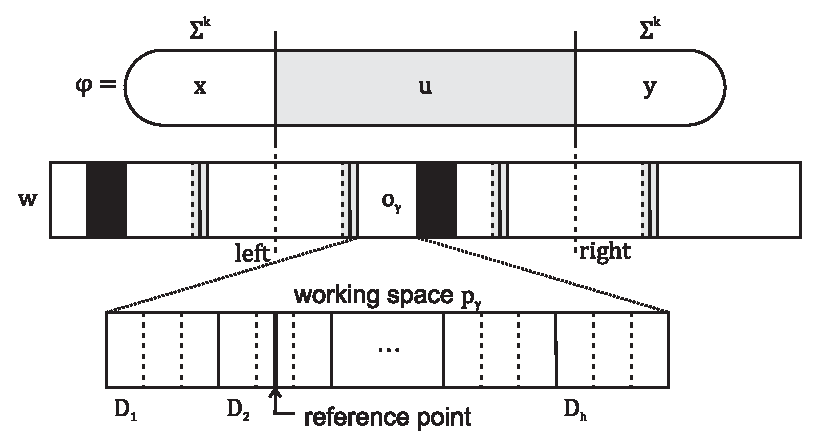
\includegraphics[scale=1.0]{img/instruction_and_tape.eps}
\caption[The execution of the instruction $\phi$.]
{The execution of the instruction $\phi$.}
\label{figure:instruction_and_tape}
\end{figure}

Algorithm \ref{algorithm:dxclra_instruction} describes the execution of the instruction $\phi$ in detail. The used variables and constants will be defined later. The interpretation of the working space $p_{\gamma}$ is illustrated in Figure \ref{figure:working_space_detail}.

\begin{figure}[htp]
\centering
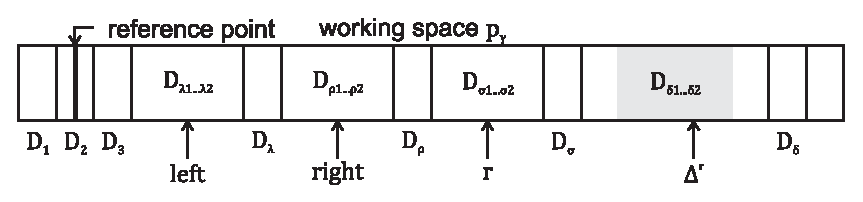
\includegraphics[scale=1.0]{img/working_space_detail.eps}
\caption[The interpretation of the working space $p_{\gamma}$.]
{The interpretation of the working space $p_{\gamma}$.}
\label{figure:working_space_detail}
\end{figure}

\begin{algorithm}
\SetKwInOut{Input}{Input}\SetKwInOut{Output}{Output}
\caption{Executing one step of the instruction $\phi$.}
\label{algorithm:dxclra_instruction}
\DontPrintSemicolon
\LinesNumbered
\Input{Word $w \in \{\lambda, \cent\} \cdot \Gamma^* \cdot \{\lambda, \$\}$, working area $o_{\gamma}$, [instruction $\phi$].}
\nonl From the following steps execute the first step, which has not been executed yet and $\textbf{Halt}$. If you encounter a conflicting step, i.\,e.\ a step which is either not possible to execute or which does not correspond to the information encoded in the working area $o_{\gamma}$, then $\textbf{Reject}$.\;
Mark the unit $D_2$. The corresponding $\Delta$ is called the {\em reference point}.\label{algorithm:dxclra_instruction_step_1}\;
\nonl Let $\textsf{left}$ be the position of the first letter of $u$ relative to the reference point, $\textsf{right}$ be the position of the last letter of $u$ relative to the reference point. Compute $j$ and $s = m_0 + m_2 (i - 1) + (j - 1)$. If the instruction $\phi$ is not provided at the input, compute these values from the information encoded in the corresponding units. If it is not possible, i.\,e.\ the units $D_{\lambda}$, $D_{\rho}$, $D_{\sigma}$, $D_{\delta}$ have not been marked yet, $\textbf{Reject}$.\;
Encode $\textsf{left}$ into the units $D_{\lambda_1}, \ldots, D_{\lambda_2}$. Mark the unit $D_{\lambda}$.\label{algorithm:dxclra_instruction_step_2}\;
Encode $\textsf{right}$ into the units $D_{\rho_1}, \ldots, D_{\rho_2}$. Mark the unit  $D_{\rho}$.\label{algorithm:dxclra_instruction_step_3}\;
Encode $s$ into the units $D_{\sigma_1}, \ldots, D_{\sigma_2}$. Mark the unit $D_{\sigma}$.\label{algorithm:dxclra_instruction_step_4}\;
Mark the unit $D_{\delta}$.\label{algorithm:dxclra_instruction_step_5}\;
Encode the segment $\Delta^r$ (with holes) into the units $D_{\delta_1}, \ldots, D_{\delta_2}$.\label{algorithm:dxclra_instruction_step_6}\;
Clear all letters from the end of the segment $\Delta^r$ (with holes) to the position $\textsf{right}$.\label{algorithm:dxclra_instruction_step_7}\;
Clear all letters from the position $\textsf{left}$ to the beginning of the segment $\Delta^r$ (with holes).\label{algorithm:dxclra_instruction_step_8}\;
\end{algorithm}

Algorithm \ref{algorithm:dxclra_instruction} is designed in such a way, that at any time it is possible to determine unambiguously which steps have already been executed and which are still pending. Every step of the algorithm is consistent with some instruction $\phi$ of the automaton $M$,  therefore, the solver cannot accept more than $M$. We will show later that it is possible to define the parameters and constants used in the solver in such a way, that every instruction of $M$ can be simulated by the solver. Moreover, by using the length-reducing version of coding it is possible to obtain a length-reducing version of the solver, which shortens the word in every step.

The reference point not only reserves the working area $o_{\gamma}$ (the units $D_1$ and $D_3$ must remain empty), but it also exactly defines the relative positions of the first and the last letter of the word $u$. The number $\textsf{left}$ is defined as the number of letters of the shortest prefix of $u$ containing the reference point. By analogy, the number $\textsf{right}$ is defined as the number of letters of the shortest suffix of $u$ containing the reference point.

Steps \ref{algorithm:dxclra_instruction_step_1} to \ref{algorithm:dxclra_instruction_step_5} are nondestructive, i.\,e.\ we are able to recover all symbols $\Delta$ created by these steps. However, when we start creating the continuous segment $\Delta^r$ (with holes) we lose the ability to recover all symbols $\Delta$ in the working area $o_{\gamma}$. Therefore, as we start creating this segment, the information specifying how to complete the execution of the instruction $\phi$ must already be completely encoded in the working area $o_{\gamma}$. We use the standard binary representation for numbers and we always encode the bits from the least significant bit to the most significant bit in a direction from left to right. For all numbers $\textsf{left}$, $\textsf{right}$, and $r$ we use a fixed number of bits. Therefore, it is easy to recognize the markings in the units $D_{\lambda}$, $D_{\rho}$, $D_{\sigma}$ and $D_{\delta}$.

If the unit $D_{\delta}$ is marked then we are in the phase of creating the segment $\Delta^r$ (with holes), i.\,e.\ Step \ref{algorithm:dxclra_instruction_step_6}. We build this segment step by step from left to right by replacing the letters in the subword $D_{\delta_1}, \ldots, D_{\delta_2}$ by the symbol $\Delta$. After completing this segment we move to the next Step \ref{algorithm:dxclra_instruction_step_7}. Note that before we execute Step \ref{algorithm:dxclra_instruction_step_7} the newly created segment $\Delta^r$ (with holes) is not a valid fixed point, since this segment is placed between two marked units (the reference point and the marked unit  $D_{\delta}$). After executing Step \ref{algorithm:dxclra_instruction_step_7} this segment becomes a valid fixed point. This is because we clear the marked unit $D_{\delta}$ and all the areas neighboring with the working area $o_{\gamma}$ are empty (if they exist). Therefore, we need to choose the parameter $j$ in such a way, that the newly defined groups of length $B$, defined by the newly created fixed point of the type $\Delta^r$ (with holes), are exactly the same groups as the original groups before executing Step \ref{algorithm:dxclra_instruction_step_7}. In Step \ref{algorithm:dxclra_instruction_step_8} this problem does not arise, because the groups of length $B$  are always defined relatively to the right of a fixed point.

We conclude this section by mentioning one specific problem concerning Step \ref{algorithm:dxclra_instruction_step_7} and Step \ref{algorithm:dxclra_instruction_step_8}. The problem is, that the position $\textsf{left}$ ($\textsf{right}$, respectively) can cross the fixed point of the type $\mathbf{u} \Delta \mathbf{v} \Delta$ (see Figure \ref{figure:delete_issue}).

\begin{figure}[htp]
\centering
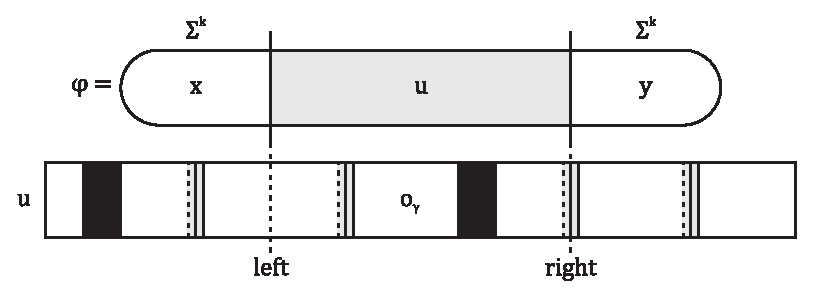
\includegraphics[scale=1.0]{img/delete_issue.eps}
\caption[Problem with the fixed point of the type $\mathbf{u} \Delta \mathbf{v} \Delta$.]
{Problem with the fixed point of the type $\mathbf{u} \Delta \mathbf{v} \Delta$.}
\label{figure:delete_issue}
\end{figure}

The positions $\textsf{left}$ and $\textsf{right}$ are fixed and we cannot change them (these positions are defined by the instruction $\phi$). Fortunately, it does not matter if we damage the fixed point of the type $\mathbf{u} \Delta \mathbf{v} \Delta$. This is because the newly created fixed point of the type $\Delta^r$ (with holes) defines the groups of length $B$ in exactly the same way as did the damaged fixed point. Moreover, thanks to the holes in the newly created fixed point we do not lose even the ability to exactly define the borders of this newly created fixed point. The only issue is that we lose the ability to recover the $\Delta$ symbol(s) of the damaged fixed point. Fortunately, these $\Delta$ symbols are close enough to the newly created segment $\Delta^r$ (with holes), so they are part of the separator corresponding to this segment. As we have already mentioned, the letters in the separator can be set arbitrarily. Therefore, if we want to recover these symbols $\Delta$ corresponding to the damaged fixed point, we can use any letter we want.

Note that the position $\textsf{left}$ ($\textsf{right}$, respectively) cannot cross the fixed point of the type $\Delta^r$ (with holes), because  the word $xuy$ covers always the whole code of the nonterminal  (including its separators).

\subsection{Choosing the Parameters}\label{section:dxclra_parameters}

In this section we define all the parameters and constants used in the previous sections. Let $\Sigma$ be a given alphabet and $G$ be a context-free grammar with $m$ nonterminals.

First we set $m_0 := 8$. Thanks to this setting, each segment $\Delta^r$ (with holes) will contain $\Delta^4$ as a subword. This is how we recognize such segments.

Each group is $B = |\Sigma|$ letters long (since we use Coding 1) and each unit is (by definition) $3 B$ letters long. The parameter $m_2$ defines the range for the parameter $j$ in Algorithm \ref{algorithm:dxclra_instruction}. Since we need this parameter $j$ only to correctly adjust the groups of length $B$ defined by the newly created fixed point, it suffices to choose $m_2 = 3 B$.

The following computations will involve the parameter $h$, which represents the number of units necessary to allow the execution of Algorithm \ref{algorithm:dxclra_instruction}.

The numbers $\textsf{left}$ and $\textsf{right}$ are bounded above by the width of the instruction $\phi$, i.\,e.\ by the constant $2c$, where $c = U + m_1 - 1$ and $U = m_0 + m_2 m - 1 + 2k$. Therefore, to encode such a number we need at most $\lceil \log_2(2c) \rceil$ units. The number $r$ is bounded above by $m_0 + m_2 m$. Observe that this upper bound depends neither on $m_1$, nor on $k$. To encode $r$ we need at most $\lceil \log_2(m_0 + m_2 m) \rceil$ units. Finally, to create the segment $\Delta^r$ (with holes) we need at most $r$ letters, i.\,e.\ at most $\lceil \frac{m_0 + m_2 m}{3 B} \rceil$ units. Therefore, we need at most
$$h = O(m_0 + m_2 m + \log(m_1 + 2k)).$$

By Lemma \ref{lemma:dxclra_t} $m_1, k = \Theta(t)$. Therefore, for any real $\alpha > 0$, there exists a big enough $t$ such that $\alpha t$ is bigger than $h$. By using this technique we can guarantee, for any instruction $\phi = (x, u \to \Delta^r, y)$, a big enough subword $v \in \Sigma^{\ge t}$ of the word $u$. This subword $v$ will guarantee us the existence of a long enough working area $o_{\gamma}$ inside this subword $v$. In our case it is not sufficient only to say that $v \in \Sigma^{\ge t}$ is long enough, because in our algorithm this subword can be interrupted by fixed points of the type $\mathbf{u} \Delta \mathbf{v} \Delta$. The fact that $v \in \Sigma^*$ only means that we are able to recover the symbols $\Delta$ of these fixed points. However, if $v$ is long enough then there will be many of these fixed points and therefore also many of the corresponding working areas. Therefore, it will always be possible to choose one such area $o_{\gamma}$ with empty neighbors.

Let us set $\alpha = \frac{1}{6} \frac{1}{3 B}$, and let $t$ be the smallest positive integer such that for the corresponding parameters $m_1$ and $k$ the following holds:
$$\frac{1}{6} \frac{1}{3 B} t > h.$$
In the first phase of our algorithm let us distribute the fixed point throughout the input working tape in such a way that the corresponding working spaces between any two consecutive fixed points contain at least $2h$ units. Since $t$ is bigger than the length of $6 h$ units, it is easy to see that we will always be able to find a long enough working area $o_{\gamma}$ inside the subword $v \in \Sigma^{\ge t}$.

Also note that during the course of our algorithm the length of every working area will be bounded from above by $2h$ units. This is because the fact that during the course of our algorithm we only replace some segments by new fixed points, so it is not possible to enlarge any working area in this way.

Finally, the constant $K$ of the querier must be long enough to enable us to see any instruction $\phi$ of $M$ as a whole, plus some extra working spaces on both sides of this instruction. It is sufficient to set $K = O(c + h) = O(c)$.

\subsection{Length-Reducing Algorithm}\label{section:dxclra_length-reducing}

In is not difficult to modify Algorithms \ref{algorithm:dxclra_solver} and \ref{algorithm:dxclra_instruction} in order to work with the length-reducing version of Coding 1 (see Section \ref{section:dxclra_coding}). We only need to redefine the length of the word $| \cdot |$ to a weighted sum of its letters, where the letters from $\Sigma$ have the weight $1$ and the symbol $\Delta$ has the weight equal to $\kappa + 1$, where $\kappa$ is the reduction factor from $\kappa$-Reducing Coding 1 Theorem \ref{theorem:dxclra_k_reducing_coding_1}. Moreover, in order to create the segment $\Delta^r$ (with holes) we need now $(\kappa + 1)$ times more letters, i.\,e.\ (at most) $(\kappa + 1) (m_0 + m_2 m)$ letters. When we create the segment $\Delta^r$ (with holes) we always rewrite $\kappa + 1$ consecutive letters from $\Sigma$ to one symbol $\Delta$. It is easy to see that the constant $\kappa$ can be easily incorporated into the previous consideration in Section \ref{section:dxclra_parameters}.

\section{Limited Context Restarting Automata}\label{section:lcra}

The main source for this section is \cite{OCM13}, although here we use a sligthly different notation that is compatible with the rest of this thesis.

In \cite{B11} \emph{limited context restarting automata} were defined as an extension of clearing restarting automata. Also these automata apply rewrite steps only based on context information, but their rewrite rules are more general. In fact, the most general form of these automata accepts exactly the growing context-sensitive languages. In addition, in~\cite{B11} a special version of a genetic algorithm is proposed to learn these automata from positive and negative samples. Here we introduce a slightly generalized version which uses weight-reducing rules instead of length-reducing ones.

In Sections \ref{section:ordinary_lcra} and \ref{section:confluent_lcra} we study the correspondence between limited context restarting automata and McNaughton families of languages of~\cite{Beaudry2003}, among which the class \GCSL\ of \emph{growing context-sensitive languages} \cite{Buntrock19981,DW86}, the class \CRL\ of \emph{Church-Rosser languages}~\cite{MNO88}, and the class {\sf con-gen-mon-McNL} of \emph{confluent generalized monadic McNaughton languages}~\cite{Leupold2011} will appear prominently.

\begin{definition}\label{DefLCRA}[\cite{OCM13}]
A {\em limited context restarting automaton} $M$ ($\lcRA$ $M$, for short) is simply a weight-reducing context rewriting system $M=(\Sigma,\Gamma,\Phi)$ (see Definitions \ref{definition:crs} and \ref{definition:crs-types}).
\end{definition}

\begin{example}
Let $M=(\{a,b,c\},\{a,b,c\},\Phi)$ be the $\lcRA$ that is defined by the set of instruction $\Phi=\{\rarule{\lambda}{\underline{acbb}}{c}{\lambda},\rarule{\cent}{\underline{c}}{\lambda}{\$}\}$. Then $aa\underline{acbb}bbbb \vdash_M a\underline{acbb}bb \vdash_M \underline{acbb} \vdash_M \underline{c} \vdash_M \lambda$, and so the word $a^3cb^6$ belongs to $L(M)$. It is easily seen that $L(M) = \{\, a^ncb^{2n} \mid n \ge 0 \,\}$.
\end{example}

Recall from Definition~\ref{DefLCRA} that all instructions of an $\lcRA$ are necessarily weight-reducing. These most general $\lcRA$ are said to be of type~$\mathcal{R}_0'$. We now define some restricted types of $\lcRA$ by putting additional restrictions on the form of their instructions. We say that an $\lcRA$ $M=(\Sigma,\Gamma,\Phi)$ is of type

\begin{itemize}
\item[$\bullet\;\mathcal{R}_1'$,] if for every $\rarule{u}{x}{y}{v} \in \Phi$: $|y|\le 1$, and $x \in \Gamma^+$;
\item[$\bullet\;\mathcal{R}_2'$,] if for every $\rarule{u}{x}{y}{v} \in \Phi$: $|y|\le 1$, $u \in \{\lambda,\leftsentinel\}$, $v \in \{\lambda,\rightsentinel\}$, and $x \in \Gamma^+$;
\item[$\bullet\;\mathcal{R}_3'$,]  if $\Phi$ only contains instructions of the form $\rarule{u}{x}{y}{\rightsentinel}$, where $|y|\le 1$, $u \in \{\lambda,\leftsentinel\}$, and $x \in \Gamma^+$;
\end{itemize}

We say that an $\lcRA$ $M=(\Sigma,\Gamma,\Phi)$ is of type $\mathcal{R}_i$, for $i \in \{0, 1, 2, 3\}$, if $M$ is of type $\mathcal{R}_i'$ and $\Phi$ only contains length-reducing instructions.

\subsection{Restricted Types}\label{section:ordinary_lcra}

For any $\mathcal{R} \in \{\mathcal{R}_0,\mathcal{R}_0',\mathcal{R}_1,\mathcal{R}_1',\mathcal{R}_2,\mathcal{R}_2',\mathcal{R}_3,\mathcal{R}_3'\}$, we will refer to $\lcRA$ of type $\mathcal{R}$ as ${\lcRA}[\mathcal{R}]$. In~\cite{B10Diploma}, Basovn{\'\i}k  studied length-reducing $\lcRA$, obtaining the following three characterizations.

\begin{theorem}{\rm \cite{B10Diploma}}\label{ThmBasovnik} \\[+0.2cm]
${\rm (a)}\;  {\mathcal L}(\lcRA[0]) = \GCSL.\;
{\rm (b)}\; {\mathcal L}(\lcRA[2]) = \CFL.\;
{\rm (c)}\; {\mathcal L}(\lcRA[3]) = \Reg.$
\end{theorem}

In the current section we complete these results by also studying the other five types of $\lcRA$.
\vspace{+0.2cm}

Let $M = (\Sigma,\Gamma,\Phi)$ be an $\lcRA$. With $M$ we can associate the finite string-rewriting system $R(M) = \{\,uxv\to uyv\mid \rarule{u}{x}{y}{v}\in \Phi\,\}.$ Then $R(M)$ induces a \emph{reduction relation} $\Rightarrow_{R(M)}^*$ on the set of bordered words $\cent\cdot\Gamma^*\cdot\$$, which is the reflexive and transitive closure of the \emph{single-step reduction relation} $\Rightarrow_{R(M)}$ 
that is defined as follows:
$$\begin{array}{c}
\cent w\$\Rightarrow_{R(M)}\cent z\$
\text{ iff }\\
\exists \alpha,\beta\in(\Gamma\cup\{\cent,\$\})^*\,\exists (\ell\to r)\in R(M):
   \cent w\$ = \alpha \ell\beta \textup{ and } \cent z\$ = \alpha r\beta.
\end{array}$$
Thus, for all $w,z\in\Gamma^*$, we have $\cent w\$ \Rightarrow_{R(M)}\cent z\$$ iff $w \vdash_M z$ holds. Accordingly, we see that
$$L(M) = \{\,w\in\Sigma^*\mid w\vdash_M^*\lambda\,\}
       = \{\,w\in\Sigma^*\mid \cent w\$\Rightarrow_{R(M)}^*\cent \$\,\}.$$
By taking $S(M) = R(M) \cup \{\cent \$\to Y\}$, where $Y$ is a new letter, we obtain a finite string-rewriting system on $\Gamma'=\Gamma\cup\{\cent,\$,Y\}$ such that $L(M) = \{\,w\in\Sigma^*\mid \cent w\$ \Rightarrow_{S(M)}^*Y\,\}$ holds. It follows that $L(M)$ is the \emph{McNaughton language} that is specified by the four-tuple $(S(M),\cent,\$,Y)$.
\vspace{+0.2cm}

If $M$ is of type $\mathcal{R}_0'$, then the string-rewriting system $S(M)$ is weight-reducing. Hence, it follows from Theorem~\ref{ThmMcNL}(a) that $L(M)\in\GCSL$. In fact, we will establish the following characterization, extending Theorem~\ref{ThmBasovnik}(a).

\begin{theorem}\label{PropR0}
${\mathcal L}(\lcRAp[0]) = {\mathcal L}(\lcRA[0]) =  \GCSL.$
\end{theorem}

\noindent
\begin{proof}
Because of the above observation, it suffices to show that each growing context-sensitive language is accepted by some $\lcRA$ of type~$\mathcal{R}_0$. Hence, assume that $L\subseteq\Sigma^*$ is growing context-sensitive. We construct an $\lcRA[0]$ $M$ for~$L$. As $L$ is growing context-sensitive, there exists a length-reducing two-pushdown automaton (\TPDA, for short, see, e.\,g.,~\cite{Buntrock19981}) $T = (Q,\Sigma,\Gamma,\delta,$ $q_0,\bot,\lambda,\lambda,\{q_f\})$ that accepts~$L$. Here $\Gamma$ is the tape alphabet of $T$ that includes the input alphabet $\Sigma$ as well as the special bottom marker~$\bot$ for the pushdowns. Thus, for all $w\in\Sigma^*$, $w\in L$ if and only if $T$ accepts starting from the initial configuration $\bot q_0w\bot$, that is, if and only if $\bot q_0 w\bot\vdash_T^* q_f$ holds (see \cite{N2005} Lemma 3.4 and Lemma 4.1). Actually, we may even assume without loss of generality that the initial step of a computation of $T$ that starts from an initial configuration of the form $\bot q_0w\bot$ reduces the overall length of the configuration by at least two, and that $T$ never enters its initial state $q_0$ during a computation.

Let $\overline{\Gamma}=\{\,\overline{a} \mid a\in  \Gamma\,\}$ be a new alphabet in one-to-one correspondence to $\Gamma$ such that $Q$, $\Gamma$, and $\overline{\Gamma}$ are pairwise disjoint, let $\overline{\phantom{a}}:\Gamma^*\to {\overline{\Gamma}}^*$ denote the corresponding isomorphism that is induced by $a\mapsto\overline{a}$ ($a\in\Gamma$), and let $\Delta = Q\cup\Gamma \cup \overline{\Gamma}$. In analogy to the proof of \cite{N2005} Lemma 4.1, we can construct a finite length-reducing string-rewriting system $R$ on $\Delta$ such that, for all $w\in\Sigma^*$, $w\in L \textup{ iff }  \overline{\bot}q_0w\bot \Rightarrow_R^*q_f.$ Here the final state $q_f$ is introduced by specific rules of the form $\overline{\bot} \overline{u} qv\bot \to q_f$. Now from~$R$ we obtain an $\lcRA$ $M = (\Sigma,\Delta,\Phi)$ by taking
$$\begin{array}{lcl}
\Phi  & = &\{\,(\lambda, \ell\to r, \lambda)\mid (\ell\to r)\in R,|\ell|_{\overline{\bot}}=|\ell|_\bot=0\,\}\;\cup\\
      &   &\{\,(\cent, u\to v, \lambda)\mid (\overline{\bot}u\to \overline{\bot}v)\in R, |u|_\bot = 0 =|u|_{q_0}\, \}\;\cup\\
%\end{array}$$
%$$\begin{array}{lcl}   
   &   &\{\,(\cent, u\to v, \lambda)\mid (\overline{\bot}q_0u\to \overline{\bot}v)\in R, |u|_\bot = 0\, \}\;\cup\\
   &   &\{\,(\lambda, u\to v, \$)\mid (u\bot\to v\bot)\in R, |u|_{\overline{\bot}} = 0\, \}\;\cup\\
%\end{array}$$
%$$\begin{array}{lcl}   
   &   &\{\,(\cent, u\to v, \$)\mid (\overline{\bot}u\bot\to \overline{\bot}v\bot)\in R, |u|_{q_0}=0\, \}\;\cup\\
   &   &\{\,(\cent, u\to v, \$)\mid (\overline{\bot}q_0u\bot\to \overline{\bot}v\bot)\in R\, \}\;\cup\\
%\end{array}$$
%$$\begin{array}{lcl}  
   &   &\{\,(\cent, u\to \lambda, \$)\mid (\overline{\bot}q_0u\bot\to q_f)\in R,|u|>0 \}\;\cup\\
   &   &\{\,(\cent, u\to\lambda,\$) \mid (\overline{\bot}u\bot\to q_f)\in R, |u|_{q_0}=0\,\}.\\
\end{array}$$
Then $M$ is of type $\mathcal{R}_0$, and for all $w\in\Sigma^+$,
$$w\in L(M) \;\Leftrightarrow\;  w\vdash_M^*\lambda
            \;\Leftrightarrow\;  \cent w\$ \Rightarrow_{R(M)}^* \cent \$
            \;\Leftrightarrow\;  \overline{\bot}q_0 w\bot \Rightarrow_R^* q_f
            \;\Leftrightarrow\;  w\in L.$$
Thus, $L(M)\, \dot{=}\, L$. This completes the proof of Theorem~\ref{PropR0}.
\end{proof}

Let $G=(N,T,S,P)$ be a weight-increasing context-sensitive grammar, that is, there exists a weight function $g$ such that $g(\ell) < g(r)$ for each rule $(\ell\to r)$ of $P$, and in addition, each rule $(\ell\to r)$ has the form $\ell=uAv$ and $r=uxv$ for some $A\in N$, $u,v\in(N\cup T)^*$, and $x\in (N\cup T)^+$. By taking
$$\Phi(G)  =  \{\,\rarule{u}{x}{A}{v} \mid (uAv\to uxv)\in P\,\}\; \cup
              \{\,\rarule{\cent}{r}{\lambda}{\$} \mid (S\to r)\in P\,\},$$
we obtain an $\lcRA$ $M(G) = (T,N\cup T,\Phi(G))$. It is easily seen that $M(G)$ is of type $\mathcal{R}_1'$, and that $L(M(G))$ $ = L(G)\cup\{\lambda\}$ holds. Thus, ignoring the special case of the empty word we see that all languages that are generated by weight-increasing context-sensitive languages are accepted by \lcRAp[1]. However, the class of languages that are generated by weight-increasing context-sensitive grammars, which is known as the class $\ACSL$ of \emph{acyclic context-sensitive languages}, coincides with the class \GCSL\ of growing context-sensitive languages~\cite{NiWo01}. Hence, we obtain the following characterization.

\begin{theorem}\label{PropR1a}
${\mathcal L}(\lcRAp[1]) =  \GCSL.$
\end{theorem}

If $M = (\Sigma,\Gamma,\Phi)$ is an $\lcRA[1]$, then the rules of $R(M)$ have the form $(uxv \to uyv)$, where $|x|>|y|$ and $|y|\le 1$. By replacing each instruction of the form $\rarule{u}{x}{\lambda}{v}\in \Phi$ by finitely many rules with a revised context, the following technical result can be derived.

\begin{lemma}\label{LemR1a}
If $M = (\Sigma,\Gamma,\Phi)$ is an $\lcRA[1]$, then there exists an equivalent $\lcRA$ $M'=(\Sigma,\Gamma,\Phi')$ of type $\mathcal{R}_1$ such that $|y|=1$ for all instructions $\rarule{u}{x}{y}{v}\in \Phi'$ satisfying $u\not=\cent$ or $v\not=\$$. In fact, for all $w,z\in \Gamma^*$, $w\vdash_M z$ if and only if $w\vdash_{M'} z$.
\end{lemma}

\begin{proof}
To obtain $M'$ from $M$, we simply replace each instruction of the form $\phi=\rarule{u}{x}{\lambda}{v}\in \Phi$. If $u=u_1A$ for some $A\in\Gamma$, then we replace $\phi$ by the instruction $\phi'=\rarule{u_1}{Ax}{A}{v}$; if $u=\lambda$ or $u=\cent$ and $v=Bv_1$ for some $B\in\Gamma$, then we replace $\phi$ by the instruction $\phi'=\rarule{u}{xB}{B}{v_1}$; if $u =\cent$ and $v=\lambda$, then we replace $\phi$ by the set of instructions $\Phi'(\phi) = \{\,\rarule{\cent}{xA}{A}{\lambda}\mid A\in \Gamma\,\} \,\cup\,\{\rarule{\cent}{x}{\lambda}{\$}\}$; if $u=\lambda$ and $v=\$$, then we replace $\phi$ by the set of instructions $\Phi'(\phi) = \{\,\rarule{\lambda}{Ax}{A}{\$}\mid A\in \Gamma\,\} \,\cup\,\{\rarule{\cent}{x}{\lambda}{\$}\}$; and if $u=\lambda=v$, then we replace $\phi$ by the set of instructions $\Phi'(\phi) = \{\,\rarule{\lambda}{xA}{A}{\lambda},\rarule{\lambda}{Ax}{A}{\lambda}\mid A\in \Gamma\,\} \,\cup\,\{\rarule{\cent}{x}{\lambda}{\$}\}$. Then, for all $w,z\in\Gamma^*$, if $w\vdash_M z$ using instruction~$\phi$, then $w\vdash_{M'} z$ by instruction $\phi'$ or by one of the instructions of $\Phi'(\phi)$, and conversely, if $w\vdash_{M'} z$ by instruction $\phi'$ or by one of the instructions of $\Phi'(\phi)$, then $w\vdash_M z$ by instruction~$\phi$.
\end{proof}

Let $M=(\Sigma,\Gamma,\Phi)$ be an $\lcRA[1]$ that satisfies the properties of Lemma~\ref{LemR1a}, let $R(M)$ be the corresponding string-rewriting system, and let $R(M)^{-1}$ denote the system $R(M)^{-1} = \{\,(v\to u) \mid (u\to v)\in R(M)\,\}.$ From $R(M)^{-1}$ we can construct a length-increasing context-sensitive grammar $G(M) = (\Gamma',\Sigma',S,R')$ that generates the language $L(G(M)) = \cent\cdot L(M)\cdot\$$. Thus, the language $\cent\cdot L(M)\cdot\$$ is a growing acyclic context-sensitive language  (see, e.\,g.,~\cite{NiWo01}). It is known from~\cite{BunHabil} that the class $\GACSL$ of \emph{growing acyclic context-sensitive languages} is closed under the operations of removing left and right end markers. Hence, the language $L(M)$ is growing acyclic context-sensitive, too. Conversely, if $G=(N,T,S,P)$ is a length-increasing context-sensitive grammar, then by taking
$$
\Phi(G)  =  \{\,\rarule{u}{x}{A}{v} \mid (uAv\to uxv)\in P\,\}\; \cup
            \{\,\rarule{\cent}{r}{\lambda}{\$}\mid (S\to r)\in P\,\},
$$
we obtain an $\lcRA$ $M(G) = (T,N\cup T,\Phi(G))$ of type $\mathcal{R}_1$ such that $L(M(G)) = L(G)\cup\{\lambda\}$ holds. Thus,  we have the following characterization.

\begin{theorem}\label{PropR1b}
${\mathcal L}(\lcRA[1]) = \GACSL.$
\end{theorem}

It is known that the class $\GACSL$ properly contains the class $\CFL$ of context-free languages, and it is obviously contained in $\ACSL = \GCSL$. However, it is an open problem whether this containment is strict or not.
\vspace{+0.1cm}

Let $M = (\Sigma,\Gamma,\Phi)$ be an \lcRA[2']. Then, for each instruction $\rarule{u}{x}{y}{v}\in \Phi$, we have $u\in\{\lambda,\cent\}$, $v\in\{\lambda,\$\}$, $|x|\ge 1$, $|y|\le 1$, and $g(x)>g(y)$ for a fixed weight function~$g$. Hence, the corresponding string-rewriting system $R(M)$ can be split into four disjoint subsystems:
$$\begin{array}{llcll}
{\rm (a)} & R_{bif} & = & \{\,\cent x\$ \to \cent y\$ \mid \rarule{\cent}{x}{y}{\$}\in \Phi\,\}, & \textup{the \emph{bifix rules} of }R(M),\\
{\rm (b)} & R_{pre}& = & \{\,\cent x \to \cent y \mid \rarule{\cent}{x}{y}{\lambda}\in \Phi\,\}, & \textup{the \emph{prefix rules} of }R(M),\\
{\rm (c)} & R_{suf}& = & \{\,x\$ \to y\$ \mid \rarule{\lambda}{x}{y}{\$}\in \Phi\,\}, & \textup{the \emph{suffix rules} of }R(M),\\
{\rm (d)} & R_{inf}& = & \{\,x \to y \mid \rarule{\lambda}{x}{y}{\lambda}\in \Phi\,\}, & \textup{the \emph{infix rules} of }R(M).\\
\end{array}$$
Let $B(M) = \{\,\alpha\in\Gamma^*\mid \cent \alpha\$\in {\rm dom}(R_{bif}) \textup{ and }
\cent \alpha\$\Rightarrow_{R(M)}^* \cent \$\,\}\,\cup\,\{\lambda\}.$ As $R(M)$ is finite, so is the set~$B(M)$. Let $R' = R_{pre}\cup R_{suf}\cup R_{inf}$. Then
$$
L(M)  =   \{\,w\in\Sigma^*\mid \cent w\$\Rightarrow_{R(M)}^*\cent\$\,\}
      =   \{\,w\in\Sigma^*\mid \exists \alpha\in B(M):\cent w\$\Rightarrow_{R'}^*\cent \alpha\$\,\},
$$
that is, $\cent\cdot L(M) \cdot \$ = \nabla_{R'}^*(\cent\cdot B(M)\cdot\$) \cap (\cent\cdot\Sigma^*\cdot\$),$ where $\nabla_{R'}^*(\alpha)$ denotes the \emph{set of ancestors} of $\alpha$ mod~$R'$, and $\nabla_{R'}^*(B) = \bigcup_{\alpha\in B}\nabla_{R'}^*(\alpha)$ for any set~$B$. Now we define a mixed rewriting system (see, e.\,g.,~\cite{Hofbauer2004301}) $P(M)=P_{pre}\cup P_{suf}\cup P_{inf}$ by taking the {\em prefix-rewriting system}\footnote{The rules of a prefix-rewriting system can only be applied to the prefix of a word.} $P_{pre}  =  \{\,x \to  y \mid (\cent x\to \cent y)\in R_{pre}\,\}$, the {\em suffix-rewriting system}\footnote{The rules of a suffix-rewriting system can only be applied to the suffix of a word.} $ P_{suf}  =  \{\,x \to  y \mid (x\$\to y\$)\in R_{suf}\,\}$, and the {\em string-rewriting system}  $P_{inf}  =  R_{inf}$. Then $L(M) = \nabla_{P(M)}^*(B(M))\cap\Sigma^*.$ As $P(M)$ only contains \emph{generalized monadic rules} (see, e.\,g.,~\cite{Leupold2011}), it follows that the set $\nabla_{P(M)}^*(B(M))$ is context-free, which in turn implies that $L(M)$ is a context-free language.

Conversely, if $L\subseteq\Sigma^*$ is a context-free language, then there exists a context-free grammar $G=(N,\Sigma,S,P)$ for $L\cap\Sigma^{\ge 2}$ such that, for each rule $(\ell\to r)$ of $P$, we have $|\ell|=1$ and $|r|=2$. We now obtain an $\lcRA$ $M(G)=(\Sigma,N\cup\Sigma,\Phi)$ by taking
$$\Phi = \{\,\rarule{\lambda}{r}{\ell}{\lambda}\mid (\ell\to r)\in P\,\}\,\cup\,
         \{\,\rarule{\cent}{a}{\lambda}{\$}\mid a\in(\Sigma\cap L)\cup\{S\}\,\}.$$
Then $M(G)$ is of type $\mathcal{R}_2$, and $L(M(G))\,\dot{=}\,L$. Thus, we have the following characterization.
\begin{theorem}\label{PropR2}
${\mathcal L}(\lcRAp[2]) = {\mathcal L}(\lcRA[2]) = \CFL.$
\end{theorem}

\begin{figure}
{\small
\[ \xymatrix@R8pt@C5pt{
\txt{${\mathcal L}(\textup{\sf lc-RA}[{\mathcal R}_0])$}\ar@{=}[r] &
\txt{${\mathcal L}(\textup{\sf lc-RA}[{\mathcal R}_0'])$}\ar@{=}[r] & \txt{\sf GCSL} \ar@{=}[r]
                   & \txt{$\textup{\sf lr-McNL}$}\ar@{=}[r] & \txt{$\textup{\sf wr-McNL}$}\\
                                                           &
\txt{${\mathcal L}(\textup{\sf lc-RA}[{\mathcal R}_1'])$}\ar@{=}[u]  \\
                                                           &
\txt{${\mathcal L}(\textup{\sf lc-RA}[{\mathcal R}_1])$} \ar@{->}_?[u]  
                   & \GACSL\ar@{=}[l]\ar@{->}_?[uu]\\
\txt{${\mathcal L}(\textup{\sf lc-RA}[{\mathcal R}_2])$}\ar@{=}[r] &
\txt{${\mathcal L}(\textup{\sf lc-RA}[{\mathcal R}_2'])$}\ar@{=}[r] &
\txt{\sf CFL}\ar@{->}[u]\ar@{=}[r] 
& \txt{$\textup{\sf mon-McNL}$}\ar@{=}[r] & \txt{$\textup{\sf gen-mon-McNL}$}\\
\txt{${\mathcal L}(\textup{\sf lc-RA}[{\mathcal R}_3])$}\ar@{=}[r] &
\txt{${\mathcal L}(\textup{\sf lc-RA}[{\mathcal R}_3'])$}\ar@{=}[r] &
\txt{\sf REG}\ar@{->}[u]\\
}
\]
\caption{Hierarchy of language classes that are accepted by the various types of
limited context restarting automata.
Question marks indicate inclusions not known to be proper.}\label{Fig1}
}
\end{figure}

Finally, let $M = (\Sigma,\Gamma,\Phi)$ be an $\lcRA[3']$, that is, for all instructions $\rarule{u}{x}{y}{v}\in \Phi$, we have $u\in\{\lambda,\cent\}$, $v=\$$, $|x|\ge 1$, $|y|\le 1$, and $g(x)>g(y)$ for a fixed weight function~$g$. Hence, the corresponding string-rewriting system $R(M)$ can be split into two disjoint subsystems:
$$\begin{array}{llcll}
{\rm (a)} & R_{bif} & = & \{\,\cent x\$ \to \cent y\$ \mid \rarule{\cent}{x}{y}{\$}\in \Phi\,\}, & \textup{the \emph{bifix rules} of }R(M),\\
{\rm (b)} & R_{suf}& = & \{\,x\$ \to y\$ \mid \rarule{\lambda}{x}{y}{\$}\in \Phi\,\}, & \textup{the \emph{suffix rules} of }R(M).\\
\end{array}$$
As above, the set $B(M) = \{\,\alpha\in\Gamma^*\mid \cent \alpha\$\in {\rm dom}(R_{bif}) \textup{ and } \cent \alpha\$\Rightarrow_{R(M)}^* \cent \$\,\}\,\cup\,\{\lambda\}$ is finite, and
$$
L(M)  =  \{\,w\in\Sigma^*\mid \cent w\$\Rightarrow_{R(M)}^*\cent\$\,\}
      =  \{\,w\in\Sigma^*\mid \exists \alpha\in B(M):\cent w\$\Rightarrow_{R_{suf}}^* \cent\alpha\$\,\},
$$
that is, $\cent\cdot L(M) \cdot \$ = \nabla_{R_{suf}}^*(\cent\cdot B(M)\cdot\$) \cap (\cent\cdot\Sigma^*\cdot\$).$ For the suffix-rewriting system $P(M) = \{\,y\to x\mid (x\$\to y\$)\in R_{suf}\,\}$, we obtain $L(M) = \Delta_{P(M)}^*(B(M))\cap\Sigma^*.$ As $B(M)$ is finite, and, hence, regular, it follows that the set of descendants $\Delta_{P(M)}^*(B(M))$ of this set with respect to the suffix rewriting system $P(M)$ is regular~\cite{Buc64}, which in turn implies that $L(M)$ is regular.

Conversely, if $L\subseteq\Sigma^*$ is a regular language, then there exists a regular grammar $G=(N,\Sigma,S,P)$ for $L\cap\Sigma^{\ge 2}$ such that, for each rule $(\ell\to r)$ of $P$, we have $\ell\in N$ and $r\in \Sigma\cdot N \cup \Sigma^2$. We now obtain an $\lcRA$ $M(G)=(\Sigma,N\cup\Sigma,\Phi)$ by taking
$$\Phi = \{\,\rarule{\lambda}{r}{\ell}{\$}\mid (\ell\to r)\in P\,\}\,\cup\,
         \{\,\rarule{\cent}{a}{\lambda}{\$}\mid a\in(L\cap\Sigma)\cup\{S\}\,\}.$$
Then $M(G)$ is of type $\mathcal{R}_3$, and $L(M(G))\,\dot{=}\,L$. Thus, we have the following characterization.
\begin{theorem}\label{PropR3}
${\mathcal L}(\lcRAp[3]) = {\mathcal L}(\lcRA[3]) = \Reg.$
\end{theorem}

The results on the various $\lcRA$ are summarized by the diagram in Figure~\ref{Fig1}.

\subsection{Confluent Restricted Types}\label{section:confluent_lcra}

As defined in Definition~\ref{DefLCRA}, an $\lcRA$ $M=(\Sigma,\Gamma,\Phi)$ is a nondeterministic device. A word $w\in\Sigma^*$ belongs to the language $L(M)$ accepted by $M$, if and only if there exists a computation of $M$ that transforms the initial configuration with tape content $\cent w\$$ into the configuration with tape content~$\cent\$$. In general, there will be many different computations of $M$ that start from the configuration with tape content~$\cent w\$$, and only some of them will derive the tape content~$\cent \$$. As this phenomenon complicates the problem of deciding membership in~$L(M)$, we are interested in $\lcRA$ for which all computations from $\cent w\$$ lead to $\cent\$$, if $w\in L(M)$. Actually, as the reduction relation $\vdash_M$ corresponds to the single-step reduction relation $\Rightarrow_{R(M)}$ that is induced by the string-rewriting system $R(M)$ on the set of bordered words $\cent\cdot\Gamma^*\cdot \$$, this would lead to considering $\lcRA$ $M$ for which the string-rewriting system $R(M)$ is \emph{confluent on the congruence class} $[\cent\$]_{R(M)}$. Unfortunately, it is undecidable in general whether a finite string-rewriting system is confluent on a given congruence class, even if the given finite system only contains length-reducing rules~\cite{otto27}. Therefore, we turn to $\lcRA$ that satisfy an even stronger restriction than confluence on a particular congruence class.
%
\begin{definition}\label{DefConf}
An $\lcRA$ $M=(\Sigma,\Gamma,\Phi)$ is called \emph{confluent} if the corresponding string-rewriting system $R(M)$ is confluent.
\end{definition}

As $R(M)$ is a finite and terminating string-rewriting system for each $\lcRA$, confluence is a decidable property of $\lcRA$ (see Proposition~\ref{PropCon} and the subsequent paragraph). We illustrate the above definition by a simple example.

\begin{example}\label{ExConLcR}
 Let $\Sigma=\{a\}$, let $\Gamma = \{a,F\}$, and let 
$\Phi=\{\rarule{\cent}{aaaa}{aaF}{\lambda},$ $\rarule{\lambda}{Faa}{aF}{\lambda},
        \rarule{\lambda}{F}{\lambda}{\$},\rarule{\cent}{aa}{\lambda}{\$},\rarule{\cent}{a}{\lambda}{\$}\}.$ Then $M=(\Sigma,\Gamma,\Phi)$ is an $\lcRA$ of type $\mathcal{R}_0$ that accepts the language $L_{\rm expo}$ (see Example \ref{ExMcNL}), and it is easily checked that $M$ is confluent.
\end{example}

We will use the prefix {\sf con-} to denote types of confluent $\lcRA$. Further, for each type $\mathcal{R}\in\{\,\mathcal{R}_i',\mathcal{R}_i\mid i\in\{0,1,2,3\}\,\}$, {\sf lc-RA$[\textup{\sf con-}\mathcal{R}]$} will denote the class of $\lcRA$ of type $\mathcal{R}$ that are confluent.

In the following we study the expressive power of the various types of confluent $\lcRA$. As in the previous section we consider the various types in turn, from the most general one to the most restricted one.

If $M=(\Sigma,\Gamma,\Phi)$ is an $\conlcRA[0']$, then $S(M) = R(M) \cup  \{\cent\$\to Y\}$ is a finite weight-reducing string-rewriting system that is confluent, and $L(M)$ is simply the McNaughton language that is specified by $(S(M),\cent,\$,Y)$. Thus, $L(M)$ is a \emph{Church-Rosser language}~\cite{MNO88}. On the other hand, if $L\subseteq\Sigma^*$ is a Church-Rosser language, then it is accepted by a length-reducing deterministic two-pushdown automaton~\cite{N2005}. Following the proof of Theorem~\ref{PropR0}, a confluent $\lcRA$ of type $\mathcal{R}_0$ can be constructed for~$L$. Hence, we obtain the following characterization.
%
\begin{theorem}\label{PropConR0}
${\mathcal L}(\conlcRA[0']) = {\mathcal L}(\conlcRA[0]) = \CRL.$
\end{theorem}

In~\cite{Woi03} Woinowski introduced a normal form for presentations of Church-Rosser languages, called \emph{context-splittable Church-Rosser language systems}. Such a presentation is of the form $(S,\cent,\$,Y)$, where $S$ is a finite, weight-reducing, and confluent string-rewriting system that consists of rules of the form $(uxv\to uyv)$, where $u,v\in\Gamma^*$, $x\in\Gamma^+$, and $|y|\le 1$, and rules of the form $(\cent x\$\to Y)$, where $x\in\Gamma^+$. As each Church-Rosser language admits a presentation of this form~\cite{Woi03}, and as a presentation of this form can immediately be translated into an $\lcRA$ of type $\textup{\sf con-}\mathcal{R}_1'$, this gives the following characterization.

\begin{theorem}\label{PropConR1prim}
${\mathcal L}(\conlcRA[1']) = \CRL.$
\end{theorem}

For the class of languages that are accepted by confluent $\lcRA$ of type~$\mathcal{R}_1$,
we have no characterization result yet. On the one hand, these automata can only accept (certain) Church-Rosser languages, and hence, they do not accept all context-free languages. On the other hand, the language  $L_{\rm expo5} = \{\,a^{5^n}\mid n\ge 0\,\}$ is accepted by an $\conlcRA[1]$, as shown in~\cite{OCM12}. As this language is not context-free, we can at least conclude the following.
%
\begin{corollary}\label{CorConR1}
The language class ${\mathcal L}(\conlcRA[1])$ is incomparable to the class $\CFL$ with respect to inclusion.
\end{corollary}

It remains open whether $\lcRA$ of type $\textup{\sf con-}\mathcal{R}_1$ accept all Church-Rosser languages, in fact, it is even open whether they accept at least all deterministic context-free languages.

In the following we present the results concerning the confluent $\lcRA$ of type $\mathcal{R}_2'$ and $\mathcal{R}_2$. We do not give proofs, since these proofs are very complicated and technical. The interested reader is referred to \cite{OCM13}.

\begin{theorem}\label{congenmonMcNL}
$\mathcal{L}(\conlcRA[2']) = \textup{\sf con-gen-mon-McNL}$.
\end{theorem}
%
\begin{theorem}\label{conmonMcNL}
$\mathcal{L}(\conlcRA[2]) \subseteq \textup{\sf con-mon-McNL}$.
\end{theorem}

It currently remains open whether the converse of Theorem~\ref{conmonMcNL} holds.

Finally, we turn to the confluent $\lcRA$ of types  $\mathcal{R}_3'$ and $\mathcal{R}_3$. If $M$ is an $\conlcRA[3']$, then $L(M)$ is a regular language by Theorem~\ref{PropR3}. Conversely, if $L\subseteq\Sigma^*$ is a regular language, then there exists a $\DFA$ $A=(Q,\Sigma,q_0,F,\delta)$ that accepts~$L^R$. We define an $\lcRA$ $M=(\Sigma,Q\cup\Sigma,\Phi)$ as follows, where $a,b\in\Sigma$ and $q,q'\in Q$:
$$\begin{array}{ccl}
\Phi & = & \{\,\rarule{\cent}{ab}{q}{\lambda}  \mid  \delta(q_0,ab)=q\,\}
      \,  \cup \,  \{\,\rarule{\cent}{qa}{q'}{\lambda}  \mid  \delta(q,a)=q'\,\} \,\cup \\
     &   & \{\,\rarule{\cent}{q}{\lambda}{\$}  \mid  q\in F\,\}
      \, \cup  \, \{\,\rarule{\cent}{a}{\lambda}{\$}  \mid a\in \Sigma\cap L^R\,\}.
\end{array}$$
It is easily seen that $L(M)\,\dot{=}\,L^R$, and that the string-rewriting system $R(M)$ is confluent. By taking $M'=(\Sigma,Q\cup\Sigma,\Phi')$, where
$\Phi' = \{\,\rarule{\lambda}{u^R}{v^R}{\$} \mid \rarule{\cent}{u}{v}{\lambda}\in \Phi\,\} 
         \,\cup
         \{\,\rarule{\cent}{u^R}{v^R}{\$} \mid \rarule{\cent}{u}{v}{\$}\in \Phi\,\}$,
we obtain a confluent $\lcRA$ of type $\mathcal{R}_3$ that accepts the language~$L$. Thus, we have the following characterization.
%
\begin{theorem}\label{PropConR3}
${\mathcal L}(\conlcRA[3']) = {\mathcal L}(\conlcRA[3]) = \Reg.$
\end{theorem}

The diagram in Figure~\ref{Fig2} summarizes our results on confluent $\lcRA$.

\begin{figure}
{\small
\[ \xymatrix@R8pt@C15pt{
                              &                      &                   & \txt{\sf GCSL}\\
\txt{${\mathcal L}(\textup{\sf lc-RA}[\textup{\sf con-{$\mathcal R$}}_0])$}\ar@{=}[r] &
\txt{${\mathcal L}(\textup{\sf lc-RA}[\textup{\sf con-{$\mathcal R$}}_0'])$}\ar@{=}[r] &
\txt{\sf CRL}\ar@{->}[ur] & \txt{\sf CFL}\ar@{->}[u]\\
       &  \txt{${\mathcal L}(\textup{\sf lc-RA}[\textup{\sf con-{$\mathcal R$}}_1'])$}\ar@{=}[u] &
\txt{\sf DCFL}\ar@{->}[u]\ar@{->}[ur] \\
     \txt{${\mathcal L}(\textup{\sf lc-RA}[\textup{\sf con-{$\mathcal R$}}_1])$} \ar@{->}_?[ur]  &  &
\txt{\sf symDCFL}\ar@{->}[u]\\
      & \txt{${\mathcal L}(\textup{\sf lc-RA}[\textup{\sf con-{$\mathcal R$}}_2'])$}\ar@{->}[ur]\ar@{->}[uu]
& & \txt{\sf LIN}\ar@{->}[uuu]\\
             & \txt{$\textup{\sf con-gen-mon-McNL}$}\ar@{=}[u]\\
\txt{${\mathcal L}(\textup{\sf lc-RA}[\textup{\sf con-{$\mathcal R$}}_2])$}\ar@{->}_?[r]\ar@{->}[uuu]&
                  \txt{$\textup{\sf con-mon-McNL}$}\ar@{->}_?[u]  \\
\txt{${\mathcal L}(\textup{\sf lc-RA}[\textup{\sf con-{$\mathcal R$}}_3])$}\ar@{=}[r]\ar@{->}[u] &
\txt{${\mathcal L}(\textup{\sf lc-RA}[\textup{\sf con-{$\mathcal R$}}_3'])$}\ar@{=}[r] & \txt{\sf REG}\ar@{->}[uuuu]\ar@{->}[uuur]\\
}
\]
\caption{Hierarchy of language classes that are accepted by the various types of confluent limited context restarting automata. Question marks indicate inclusions not known to be proper.}\label{Fig2}
}
\end{figure}


\backmatter

% Ukázka použití některých konstrukcí LateXu (odkomentujte, chcete-li)
%%%% Uk{\'a}zka pou{\v z}it{\'\i} n{\v e}kter{\'y}ch konstrukc{\'\i} LaTeXu

\subsection{Uk{\'a}zka \LaTeX{}u}
\label{ssec:ukazka}

This short subsection serves as an~example of basic \LaTeX{} constructs,
which can be useful for writing a~thesis.

Let us start with lists:

\begin{itemize}
\item The logo of Matfyz is displayed in figure~\ref{fig:mff}.
\item This is subsection~\ref{ssec:ukazka}.
\item Citing literature~\citep{lamport94}.
\end{itemize}

Different kinds of dashes:
red-black (short),
pages 16--22 (middle),
$45-44$ (minus),
and this is --- as you could have expected --- a~sentence-level dash,
which is the longest.
(Note that we have follwed \verb|a| by a~tilde instead of a~space
to avoid line breaks at that place.)

\newtheorem{theorem}{Theorem}
\newtheorem*{define}{Definition}	% Definice ne{\v c}{\'\i}slujeme, proto "*"

\begin{define}
A~{\sl Tree} is a connected graph with no cycles.
\end{define}

\begin{theorem}
This theorem is false.
\end{theorem}

\begin{proof}
False theorems do not have proofs.
\end{proof}

\begin{figure}
	\centering
	
\includegraphics[width=30mm]{./img/logo.eps}
	\caption{Logo of MFF UK}
	\label{fig:mff}
\end{figure}


\chapter*{Conclusion}\label{chapter:conclusion}
\addcontentsline{toc}{chapter}{Conclusion}

In this thesis we have studied locally restricted models of restarting automata, starting with the most restricted model, the so-called clearing restarting automaton, which, based on a limited context, can only delete a substring of the current content of its tape, and then gradually extending its power either by relaxing the constraints put on its instructions, or by allowing auxiliary symbols. In the first part of the thesis we have focused solely on models without auxiliary symbols and compared them to Chomsky hierarchy. Additionally, we have developed a general learning framework, under which it is possible to effectively infer various types of $\lambda$-confluent models from informant (i.\,e.\ from positive and negative samples) under a suitable learning paradigm. In the second part of the thesis we have investigated models with auxiliary symbols, starting with the so-called $\Delta$-clearing restarting automaton and then moving on to limited context restarting automata. $\Delta$-clearing restarting automata are very limited in their operations. They can, in one step, either completely delete a subword or they can delete a subword and simultaneously mark its position by a symbol $\Delta$. Surprisingly, they can accept all context-free languages. For this purpose, we have designed a rather complicated coding of information used for encoding nonterminals during a bottom-up analysis. Limited context restarting automata, on the other hand, can use any number of auxiliary symbols. We have compared them with certain McNaughton families of languages and proved that the class of growing context-sensitive languages is an upper bound for all the types of limited context restarting automata considered, and that this upper bound is attained by three classes of these automata. Under the additional requirement of confluence, the Church-Rosser languages form an upper bound, which is reached by the three most general types of these automata. On the other hand, for the most restricted types of limited context restarting automata, we just obtain the regular languages, both in the confluent and the non-confluent case.

%%% Seznam použité literatury	
\def\bibname{Bibliography}
%\bibliographystyle{plain}
%FM \bibliographystyle{these}
\bibliographystyle{my_splncsnat}
\bibliography{bibliography}
\addcontentsline{toc}{chapter}{\bibname}

%%% Obrazky v disertační práci, existují-li.
%\chapwithtoc{List of Figures}
\listoffigures\addcontentsline{toc}{chapter}{\listfigurename}

%%% Tabulky v disertační práci, existují-li.
%\chapwithtoc{List of Tables}
\listoftables\addcontentsline{toc}{chapter}{\listtablename}

%%% Použité zkratky v disertační práci, existují-li, včetně jejich vysvětlení.
\chapwithtoc{List of Abbreviations}

\noindent{\bf Journals and proceedings}

\begin{enumerate}[]
\item {\sf ArchMLG}: Archiv für mathematische Logik und Grundlagenforschung.
\item {\sf FI}: Fundamenta Informaticae.
\item {\sf ICOM}: Information and Computation.
\item {\sf IJFCS}: International Journal of Foundations of Computer Science.
\item {\sf JACM}: Journal of the Association for Computing Machinery.
\item {\sf JALC}: Journal of Automata, Languages and Combinatorics.
\item {\sf JCSS}: Journal of Computer and System Sciences.
\item {\sf JMLR}: Journal of Machine Learning Research.
\item {\sf LNAI}: Lecture Notes in Artificial Intelligence.
\item {\sf LNCS}: Lecture Notes in Computer Science.
\item {\sf RAIRO}: RAIRO - Theoretical Informatics and Applications.
\item {\sf TCS}: Theoretical Computer Science.
\end{enumerate}


%%% Použité symboly v disertační práci, existují-li, včetně jejich vysvětlení.
\chapwithtoc{List of Symbols}

\noindent{\bf Standard Mathematical Symbols}.

\begin{enumerate}[]
\item $\N$\ : set of (positive) natural numbers.
\end{enumerate}

\noindent{\bf Words and Languages} (see Section \ref{section:words-and-languages}).

\begin{enumerate}[]
\item $a, b, c, d$\ : symbols usually reserved for letters.
\item $u, v, w, x, y, z$\ : symbols usually reserved for words.
\item $\lambda$\ : the empty word.
\item $\Sigma$\ : usually denotes an (input) alphabet.
\item $\Gamma$\ : usually denotes a working alphabet (with auxiliary symbols).
\item $L, L_0, L_1, L_2$\ : symbols usually reserved for languages (over $\Sigma$ or $\Gamma$).
\item $=$\ : equality of numbers, sets, languages, etc.
\item $\dot{=}$\ : equality of languages up to the empty word. $L\, \dot{=}\, L' \Leftrightarrow L \cup \{\lambda\} = L' \cup \{\lambda\}$.
\item $\subseteq$\ : subset or equal.
\item $\supseteq$\ : superset or equal.
\item $\subset$\ : proper subset.
\item $\supset$\ : proper superset.
\item $\Sigma^*$\ : set of all words over $\Sigma$.
\item $\Sigma^+$\ : set of all nonempty words over $\Sigma$.
\item $\Sigma^k$\ : set of all words over $\Sigma$ of length $k$.
\item $\Sigma^{\le k}$\ : set of all words over $\Sigma$ of length at most $k$.
\item $|w|$\ : length of the word $w$.
\item $|w|_a$\ : number of occurrences of the letter $a$ in the word $w$.
\item $u \cdot v$ (or $uv$)\ : catenation (or concatenation) of the words $u$ and $v$.
\item $w^i$\ : is defined as follows\ : $w^0 = \lambda$, $w^{i+1} = w^i \cdot w$.
\item $w^R$\ : reversal (mirror image) of a word $w$.
\item $\Pref_k(u)$\ : prefix of length $k$ of the word $u$.
\item $\Suff_k(u)$\ : suffix of length $k$ of the word $u$.
\item $\Int_k(u)$\ : interior words of length $k$ that occur in $u$.
\item $L_1 \cup L_2$\ : union of languages $L_1$ and $L_2$.
\item $L_1 \cap L_2$\ : intersection of languages $L_1$ and $L_2$.
\item $L_1 \cdot L_2$ (or $L_1 L_2$)\ : catenation (or concatenation) of languages $L_1$ and $L_2$.
\item $L^i$\ : is defined as follows\ : $L^0 = \{\lambda\}$, $L^{i+1} = L^i \cdot L$.
\item $L^*$ ($L^+$, respectively)\ : Kleene star (Kleene plus, respectively) of a language $L$.
\item $L^R$\ : reversal (mirror image) of a language $L$.
\item $\delta_x(L) = x \backslash L$\ : left-derivate of $L$ with respect to $x \in \Sigma^*$.
\item $\delta^x(L) = L / x$\ : right-derivate of $L$ with respect to $x \in \Sigma^*$.
\item $L_0 \backslash L$\ : left-quotient of $L$ by $L_0$.
\item $L / L_0$\ : right-quotient of $L$ by $L_0$.
\item $2^S$ (or $\mathcal{P}(S)$)\ : power set of $S$, i.\,e.\ the collection of all subsets of $S$.
\item $\calLL$\ : set of languages.
\item $\calM$\ : set of models (automata, grammars, context rewriting systems, etc.).
\item $\calL{\calM}$\ : set of languages accepted (recognized, generated, etc.) by the set of models (automata, grammars, context rewriting systems, etc.) $\calM$.
\item $\calA$\ : symbol denoting an algorithm.
\item $\Fin$\ : finite languages.
\end{enumerate}

\noindent{\bf Regular Languages} (see Section \ref{section:regular-languages}).

\begin{enumerate}[]
\item $\Reg$\ : regular languages.
\end{enumerate}

\noindent{\em Finite Automata} (see Section \ref{subsection:finite-automata}).

\begin{enumerate}[]
\item $A$\ : usually denotes a finite automaton.
\item $Q$\ : usually denotes a finite set of states.
\item $\FA$\ : finite automaton.
\item $\DFA$\ : deterministic finite automaton.
\item $\NFA$\ : nondeterministic finite automaton.
\item $\lambda$-$\NFA$\ : nondeterministic finite automaton with $\lambda$-transitions.
\item $\NNFA$\ : $\NFA$ with nondeterministic starting state.
\end{enumerate}

\noindent{\bf Context-Free Languages} (see Section \ref{section:context-free-languages}).

\begin{enumerate}[]
\item $\CFL$\ : context-free languages.
\item $G$\ : usually denotes a (context-free) grammar.
\item $V_T$\ : usually denotes a set of terminals (or terminal letters).
\item $V_N$\ : usually denotes a set of nonterminals (or variables).
\item $X \to \alpha$\ : shorthand for a production $(X, \alpha)$.
\item $u \Rightarrow_G v$\ : single step derivation relation of a grammar $G$.
\item $u \Rightarrow_G^* v$\ : reflexive and transitive closure of $\Rightarrow_G$.
\item $L(G)$ or $L_G$\ : language generated by a grammar $G$.
\end{enumerate}

\noindent{\em Pushdown Machines} (see Section \ref{subsection:pushdown-machines}).

\begin{enumerate}[]
\item $\pdm$\ : pushdown machine.
\item $\pda$\ : pushdown automaton.
\item $\dpda$\ : deterministic pushdown automaton.
\item $\DCFL$\ : deterministic context-free languages.
\item $\symDCFL$\ : $\DCFL\cap\DCFL^R$.
\end{enumerate}

\noindent{\em Subfamilies} (see Section \ref{subsection:context-free-subfamilies}).

\begin{enumerate}[]
\item $\Lin$\ : linear languages.
\item $\Ocl$\ : one-counter languages.
\item $\LL(k)$-language\ : language generated by a $\LL(k)$-grammar.
\item $\LR(k)$-language\ : language generated by a $\LR(k)$-grammar.
\end{enumerate}

\noindent{\bf Chomsky Hierarchy} (see Section \ref{section:chomsky-hierarchy}).

\begin{enumerate}[]
\item $\RE$ (or $\mathcal{L}_0$)\ : recursively enumerable languages.
\item $\CSL$ (or $\mathcal{L}_1$)\ : context-sensitive languages.
\item $\CFL$ (or $\mathcal{L}_2$)\ : context-free languages.
\item $\Reg$ (or $\mathcal{L}_4$)\ : regular languages.
\end{enumerate}

\noindent{\em Context-Sensitive Grammars} (see Section \ref{subsection:context-sensitive-grammars}).

\begin{enumerate}[]
\item $\LBA$\ : linear bounded automaton.
\item $\DCSL$\ : deterministic context-sensitive languages.
\item $\GCSL$\ : growing context-sensitive languages.
\end{enumerate}

\noindent{\bf Computational Complexity Theory}.

\begin{enumerate}[]
\item $\SAT$\ : boolean satisfiability problem.
\item $\classP$\ : decision problems decidable in deterministic polynomial time.
\item $\classNP$\ : decision problems decidable in nondeterministic polynomial time.
\item $\classDSPACE(n)$\ : decision problems decidable in deterministic linear space.
\item $\classNSPACE(n)$\ : decision problems decidable in nondeterministic linear space.
\item $\classPSPACE$\ : decision problems decidable in polynomial space.
\end{enumerate}

\noindent{\bf Restarting Automata} (see Section \ref{section:restarting-automata}).

\begin{enumerate}[]
\item $\cent$\ : left marker (sentinel).
\item $\$$\ : right marker (sentinel).
\item $\MVR$\ : move-right step causes a restarting automaton to shift the read/write window one position to the right and to enter a new state.
\item $\MVL$\ : move-left step causes a restarting automaton to shift the read/write window one position to the left and to enter a new state.
\item $\Rewrite$\ : rewrite step causes a restarting automaton to replace the content of the read/write window by a new shorter string, thereby shortening the tape, and to enter state a new state. Further, the read/write window is placed immediately to the right of the new string.
\item $\Restart$\ : restart step causes a restarting automaton to place its read/write window over the left end of the tape, so that the first symbol it sees is the left border marker $\cent$, and to reenter the initial state $q_0$.
\item $\Accept$\ : accept step causes a restarting automaton to halt and accept.
\item $\RLWW$-automaton\ : the most general restarting automaton. Each cycle of each computation of an $\RLWW$-automaton $M$ consists of three phases\ : first $M$ scans its tape performing $\MVR$- and $\MVL$-instructions, then it executes a $\Rewrite$ step, and finally it scans its tape again performing $\MVR$- and $\MVL$-instructions.
\item $\RLW$-automaton\ : $\RLWW$-automaton such that its tape alphabet coincides with its input alphabet $\Sigma$, that is, no auxiliary symbols are available.
\item $\RL$-automaton\ : $\RLW$-automaton for which the right-hand side of each $\Rewrite$ step is a scattered subword of the left-hand side.
\item $\RRWW$-automaton\ : $\RLWW$-automaton that does not use any $\MVL$-steps. Thus, in each cycle an $\RRWW$-automaton can scan its tape only once from left to right.
\item $\RRW$-automaton\ : $\RRWW$-automaton such that its tape alphabet coincides with its input alphabet $\Sigma$, that is, no auxiliary symbols are available.
\item $\RR$-automaton\ : $\RRW$-automaton for which the right-hand side of each $\Rewrite$ step is a scattered subword of the left-hand side.
\item $\RWW$-automaton\ : $\RRWW$-automaton such that it makes restart immediately after performing a $\Rewrite$ operation. In particular, this means that it cannot perform a rewrite step during the tail of a computation.
\item $\RW$-automaton\ : $\RWW$-automaton such that its tape alphabet coincides with its input alphabet $\Sigma$, that is, no auxiliary symbols are available.
\item $\R$-automaton\ : $\RW$-automaton for which the right-hand side of each $\Rewrite$ step is a scattered subword of the left-hand side.
\item $\monPrefix$\ : The prefix $\monPrefix$ denotes the classes of monotone restarting automata.
\item $\detPrefix$\ : The prefix $\detPrefix$ denotes deterministic classes of restarting automata.
\end{enumerate}

\noindent{\bf String-Rewriting Systems} (see Section \ref{section:string-rewriting-systems}).

\begin{enumerate}[]
\item $\SRS$\ : string-rewriting system.
\item $R$\ : usually denotes a $\SRS$.
\item $\dom(R)$\ : domain of a $\SRS$ $R$.
\item $\rng(R)$\ : range of a $\SRS$ $R$.
\item $\|R\|$\ : size of a $\SRS$ $R$.
\item $l \to r$\ : (rewrite) rule of a $\SRS$.
\item $u \Rightarrow_R v$\ : single-step reduction relation induced by a $\SRS$ $R$.
\item $u \Rightarrow_R^* v$\ : reflexive and transitive closure of $\Rightarrow_R$.
\item $\Delta_R^*(u)$\ : set of all descendants of $u$ (modulo $\SRS$ $R$).
\item $\nabla_R^*(v)$\ : set of all ancestors of $v$ (modulo $\SRS$ $R$).
\item $\IRR(R)$\ : set of all irreducible strings (modulo $\SRS$ $R$).
\item $\CRL$\ : Church-Rosser languages.
\end{enumerate}

\noindent{\em McNaughton Families of Languages} (see Section \ref{subsection:mcnaughton-families}).

\begin{enumerate}[]
\item $\McNL$\ : McNaughton languages (defined by finite string-rewriting systems).
\item $\wrMcNL$\ : McNaughton languages defined by finite weight-reducing string-rewriting systems.
\item $\lrMcNL$\ : McNaughton languages defined by finite length-reducing string-rewriting systems.
\item $\monMcNL$\ : McNaughton languages defined by finite monadic string-rewriting systems.
\item $\genmonMcNL$\ : McNaughton languages defined by finite generalized monadic string-rewriting systems.
\item $\conMcNL$\ : McNaughton languages defined by finite confluent string-rewriting systems.
\item $\conwrMcNL$\ : McNaughton languages defined by finite confluent weight-reducing string-rewriting systems.
\item $\conlrMcNL$\ : McNaughton languages defined by finite confluent length-reducing string-rewriting systems.
\item $\conmonMcNL$\ : McNaughton languages defined by finite confluent monadic string-rewriting systems.
\item $\congenmonMcNL$\ : McNaughton languages defined by finite confluent generalized monadic string-rewriting systems.
\end{enumerate}

\noindent{\em Delimited String-Rewriting Systems} (see Section \ref{section:delimited-string-rewriting-systems}).

\begin{enumerate}[]
\item $\DSRS$\ : delimited string-rewriting system.
\item $\Apply_{\mathcal{R}}(w)$\ : string obtained by applying different rules in $\DSRS$ $\mathcal{R}$ until no more rules can be applied.
\item $\NewRule$\ : generates the next possible rule to be checked.
\item $\Consistent$\ : checks that by adding a new rule to the system, one does not rewrite a positive example and a negative example into the same string.
\end{enumerate}

\noindent{\bf Context Rewriting Systems and Derived Models} (see Section \ref{section:context-rewriting-systems} and Definitions \ref{definition:restrictions} and \ref{definition:derived-classes}).

\begin{enumerate}[]
\item $\CRS$\ : context rewriting system.
\item $\kCRS$\ : $\CRS$ with length of contexts equal to $k$.
\item $M$\ : usually denotes a $\CRS$.
\item $\calM$\ : usually denotes a set (class) of $\CRS$s.
\item $LC_k$ ($LC_{\le k}$)\ : set of left contexts of length $k$ (at most $k$).
\item $RC_k$ ($RC_{\le k}$)\ : set of right contexts of length $k$ (at most $k$).
\item $|M|$\ : width of the $\CRS$ $M$.
\item $\size(M)$\ : size of the $\CRS$ $M$.
\item $\phi = (x, z \to t, y)$\ : instruction of a $\CRS$.
\item $\vdash_M$\ : rewriting relation of the $\CRS$ $M$.
\item $\vdash^{\sf left}_M$\ : left-most rewriting relation of the $\CRS$ $M$.
\item $M_{\sf left}$\ : $\CRS$ $M$ with left-most rewriting relation $\vdash^{\sf left}_M$.
\item $\kcalM$\ : set of all $\CRS$s $M \in \calM$ such that every instruction $\phi$ of $M$ has length of contexts equal to $k$.
\item $\llcalM$\ : set of all $\CRS$s $M \in \calM$ such that every instruction $\phi$ of $M$ has width at most $l$.
\item $\klcalM$\ : set of all $\CRS$s $M \in \kcalM$ such that every instruction $\phi$ of $M$ has width at most $l$.
\item $\concalM$\ : set of all $\CRS$s $M \in \calM$ such that $M$ is confluent.
\item $\lconcalM$\ : set of all $\CRS$s $M \in \calM$ such that $M$ is $\lambda$-confluent.
\item $\leftcalM$\ : set $\{M_{\sf left} \mid M \in \calM\}$.
\item $\clRA$\ : clearing restarting automaton.
\item $\kclRA$\ : $\clRA$ with length of contexts equal to $k$.
\item $\zlclRA$\ : $\clRA$ with empty contexts and maximal width of instructions $l$.
\item $\klclRA$\ : $\clRA$ with length of contexts equal to $k$ and maximal width of instructions $l$.
\item $\sclRA$\ : subword-clearing restarting automaton.
\item $\DclRA$\ : $\Delta$-clearing restarting automaton.
\item $\kDclRA$\ : $\DclRA$ with length of contexts equal to $k$.
\item $\DXclRA$\ : $\Delta^*$-clearing restarting automaton.
\item $\kDXclRA$\ : $\DXclRA$ with length of contexts equal to $k$. 
\end{enumerate}

\noindent{\bf Other Models} (see Section \ref{section:other-models}).

\noindent{\em Marcus Contextual Grammars} (see Section \ref{section:marcus-contextual-grammars}).

\begin{enumerate}[]
\item $\phi$\ : choice mapping.
\item $\TC$\ : languages generated by total contextual grammars.
\item $\ECC$\ : languages externally generated by contextual grammars.
\item $\ICC$\ : languages internally generated by contextual grammars.
\item $\TC_c$, $\ECC_c$, $\ICC_c$\ : languages $\TC$, $\ECC$, $\ICC$ with computable choice mapping $\phi$.
\item $\EC$\ : languages externally generated by contextual grammars without choice.
\item $\IC$\ : languages internally generated by contextual grammars without choice.
\end{enumerate}

\noindent{\em Pure Grammars} (see Section \ref{section:pure-grammars}).

\begin{enumerate}[]
\item $\PCF$\ : pure context-free grammars (languages).
\item $\PLI$\ : pure length increasing grammars (languages).
\end{enumerate}

\noindent{\bf Grammatical Inference of Restricted $\CRS$} (see Chapter \ref{chapter:inference}).

\begin{enumerate}[]
\item $\Assumptions$\ : returns some set of instruction candidates.
\item $\WeakAssumptions$\ : specific example of a function $\mathsf{Assumptions}$.
\item $\StrongAssumptions$\ : specific example of a function $\mathsf{Assumptions}$.
\item $\Consistent$\ : consistency check.
\item $\Simplify$\ : simplification of the set of instructions.
\item $\Infer$\ : auxiliary inference procedure.
\item $\UnconstrainedInfer$\ : learning algorithm for $\lambda$-confluent $\CRS$s.
\end{enumerate}


\noindent{\bf $\Delta$-Clearing Restarting Automata} (see Section \ref{section:dxclra}).

\begin{enumerate}[]
\item $L_C(M)$\ : characteristic language of a $\CRS$ $M$.
\end{enumerate}

\noindent{\em Algorithmic Viewpoint} (see Section \ref{section:dxclra_viewpoint}).

\begin{enumerate}[]
\item $(Q, S)$\ : protocol consisting of a querier $Q$ and a solver $S$.
\item $L(Q, S)$ language recognized by the protocol $(Q, S)$.
\item $\calQ$\ : class of queriers.
\item $\calS$\ : class of solvers.
\item $\calL{\calQ, \calS}$\ : class of languages recognized by the queriers $\calQ$ and solvers $\calS$.
\end{enumerate}

\noindent{\bf Limited Context Restarting Automata} (see Section \ref{section:lcra}).

\begin{enumerate}[]
\item $\TPDA$\ : two-pushdown automaton.
\item $\ACSL$\ : acyclic context-sensitive languages.
\item $\GACSL$\ : growing acyclic context-sensitive languages.
\item $\lcRA$\ : limited context restarting automaton.
\item $\lcRA[i]$\ : $\lcRA$ of type~$\mathcal{R}_i$.
\item $\lcRAp[i]$\ : $\lcRA$ of type~$\mathcal{R}_i'$.
\item $\conlcRA[i]$\ : confluent $\lcRA$ of type~$\mathcal{R}_i$.
\item $\conlcRAp[i]$\ : confluent $\lcRA$ of type~$\mathcal{R}_i'$.
\end{enumerate}


%%% Přílohy k disertační práci, existují-li (různé dodatky jako výpisy programů,
%%% diagramy apod.). Každá příloha musí být alespoň jednou odkazována z vlastního
%%% textu práce. Přílohy se číslují.
%\chapwithtoc{Attachments}

\vspace{12pt}

\printindex

\openright
\end{document}
